\documentclass[12pt]{book}
\usepackage[margin=2.5cm]{geometry}
\usepackage{setspace}
\usepackage[utf8]{inputenc}
\usepackage{amsmath}
\usepackage{mathtools}
\usepackage{amsfonts}
\usepackage{amssymb} 
\usepackage{graphicx}
\usepackage{caption}
\usepackage{subcaption}
\usepackage[shortlabels]{enumitem}
\usepackage{float}
\usepackage{relsize} % for \mathlarger
\usepackage{tikz}


% version
\def \version{1} % = 0 everything
                 % = 1 hide exercises

% for red line canceling diagonally
\usepackage{cancel}
\renewcommand{\CancelColor}{\color{red}}


%% for augmented matrices, modify amsmath
\makeatletter
\renewcommand*\env@matrix[1][*\c@MaxMatrixCols c]{%
  \hskip -\arraycolsep
  \let\@ifnextchar\new@ifnextchar
  \array{#1}}
\makeatother


%%% new commands
%*************************************************
% for versions
\newcommand{\exercises}[1]{\ifnum \version=0 #1 \fi} % show exercises if version 0


%*************************************************
% for use in the \exemple command. usually #1 will be \upline and #3 will be \downline
\newcommand{\haline}
	{
	\noindent\hfill\rule{0.5\linewidth}{0.4pt}\hfill
	}	
\newcommand{\upline}
	{
	\vspace{0.5cm} \haline \vspace{0.1cm}
	}
	
\newcommand{\downline}
	{
	\vspace{0.5cm} \haline \vspace{0.1cm}
	}
%*************************************************
%Pour la numérotation des exemples
\newcounter{num_exemple}
\newcommand{\exemple}[3]
	{  \par
        \stepcounter{num_exemple} #1 \\
        \noindent
        \textbf{Example \arabic{num_exemple}} \\ 
        \noindent #2 \\
        #3
    }
%*************************************************
%Pour la numérotation des exercices
\newcounter{num_exercice}
\newcommand{\exercice}
    {   \par
        \stepcounter{num_exercice}%
        \noindent
        \textbf{Exercise \arabic{num_exercice}}:
        \quad
    }
%*************************************************
\newcommand{\theorem}[3]
	{
		\vspace{0.5cm} 
		\noindent \fbox{\begin{minipage}{\linewidth}
		\textbf{{#1}THEOREM{#2}.} #3
		\end{minipage}}
		\vspace{0.5cm}
	}
%*************************************************
\newcommand{\textcircle}[1]
	{
		\large \textcircled{\small #1} 
	}
%*************************************************

\begin{document}

% testing area
%\chapter{Introduction} \label{ch:intro}
Consider some typical mathematics problems that you've seen so far in your mathematics education. For example, an algebra exercise
\begin{align}
2x = x + 1 \quad \implies \quad x=1,
\end{align}
or to find the coordinates of the intersection of two lines
\[
	\left.
	\begin{aligned}
	y &= x+1 \\
	y &= 2x
	\end{aligned}
	\right\}
	\quad \implies 	\quad
	\begin{aligned}
	x=1 \\
	y=2
	\end{aligned}
\]
(I hope you noticed this was just a re-interpretation of the previous question). These two problems had solutions that were numbers, but we can have problems with solutions that are functions. For example the differential equations
\begin{align}
& \frac{dy}{dx} = y \quad \implies \quad y(x) = A e^x, \\
& \frac{d^2y}{dx^2} - 2 \frac{dy}{dx} + 2y = 0 \quad \implies \quad y(x) = e^x \left( A \cos 2x + B \sin 2x\right),
\end{align}
which are in fact families of functions as solutions, for any constants $A$ and $B$. Another familiar example is the solution of the quadratic equation
\begin{align}
\alpha x^2 + \beta x + \gamma \quad \implies \quad x = \frac{-\beta \pm \sqrt{\beta^2 - 4\alpha\gamma}}{2\alpha}.
\end{align}
All these previous examples have solutions that are in some sense simple. They are simple in that they have ``closed form'' solutions, meaning that you can write the solution as explicit numbers, constants representing abritrary numbers, functions like logs, exponentials, trigonometric functions, or as square roots. Such ``simple'' solutions are called \textit{analytic} solutions. Now consider the following theorem:

\theorem{ABEL-RUFFINI~}{}{There is no solution ``in radicals'' for general 5th order or higher polynomials with arbitrary coefficients.}

This theorem is also called ``Abel's impossibility theorem'' for good reason. A solution ``in radicals'' means a formula with $n$th roots in it, like the quadratic formula. Evariste Galois\footnote{Evariste Galois (1811-1832), born in Bourg-la-Reine, laid the foundations of group theory, a hugely important topic in abstract algebra with applications in quantum physics. He died at 21 years old in a duel.} found the simplest polynomial equation with no closed form expression:
\begin{align*}
x^5 - x - 1 = 0.
\end{align*}

\exemple{\upline}{
\begin{figure}[h]
	\begin{center}
	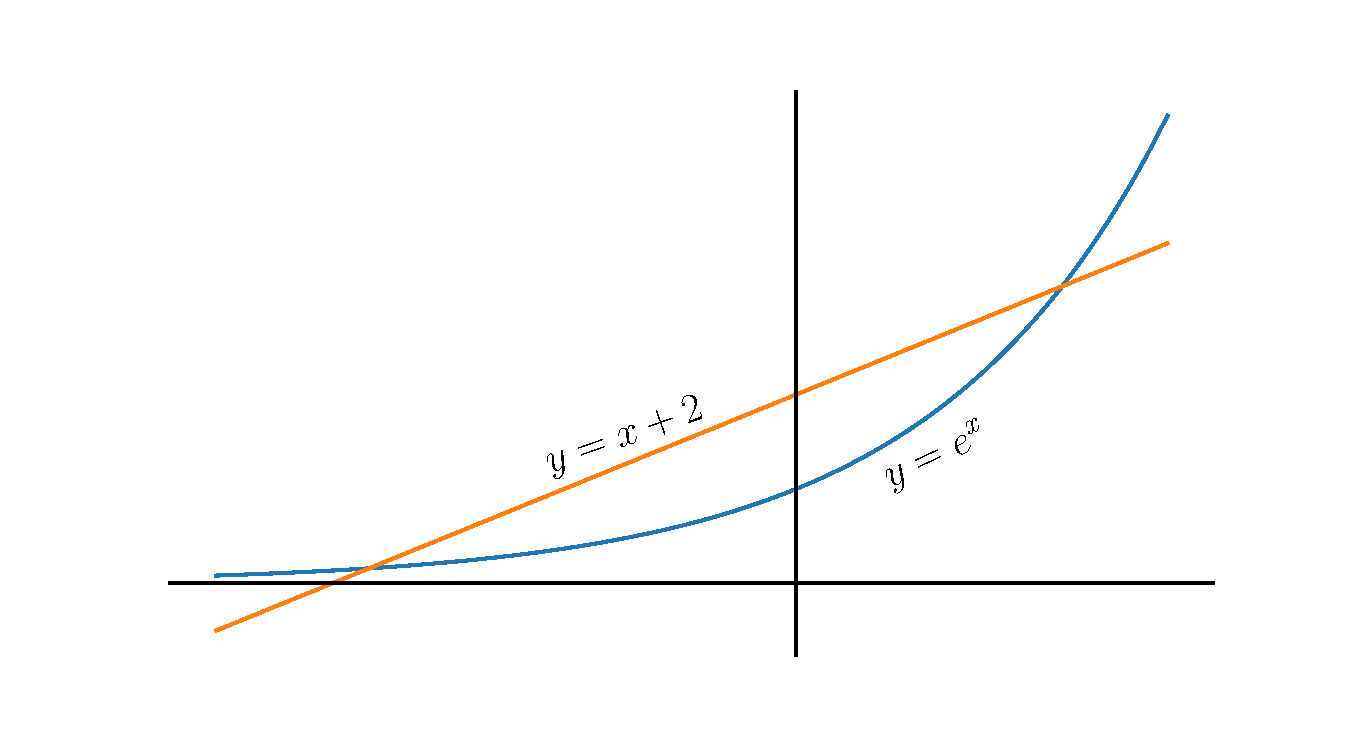
\includegraphics[width=14cm]{figures/intro_intersection.pdf} 
	  \caption{Two points of intersection.} \label{fig:intro_intersection}
	\end{center}
\end{figure}

The simple equation $e^x = x+2$ has no analytic solution. You cannot rearrange it algebraically to end up with $x=\dots$ for some closed form expression. However, it obviously has a solution (in fact 2). The solution is the intersection of two lines
\begin{align*}
y &= e^x, \quad {\rm and} \\
y &= x + 2.
\end{align*}
A simple sketch of these two lines, figure~\ref{fig:intro_intersection}, shows that the two lines must cross at 2 locations. The point is that despite having no \textit{analytic} solution, we will learn \textit{numerical} methods to solving problems like this.}{\downline}



\section{Square root of 2}
How do you know $\sqrt{2} = 1.41421356\dots$? It turns out there are many methods for finding its decimal expansion. We'll look at a few of these methods now to illustrate some basic principles of numerical analysis.


%\subsection{Taylor expansion}
%
%The Taylor\footnote{Brook Taylor (1685-1731), born in Edmonton, England. I don't know anything about this guy.} series of any infinitely differentiable function $f(x)$ at a point $a$ is given by
%\begin{align}
%f(x) = f(a) + f'(a)(x-a) + \frac{f''(a)}{2}(x-a)^2 + \cdots = \sum_{k=0}^{\infty} \frac{f^{(k)}(a)}{k!} \left( x - a \right)^k.
%\end{align}
%To use this for finding $\sqrt{2}$ we define a function
%\begin{align}
%f(x) = (1 + x)^p.
%\end{align}
%We will determine the Taylor series of this function, and then set $x=1$ and $p=1/2$ to have an infinite series giving $\sqrt{2}$. So, we consider successive derivatives
%\begin{align}
%f'(x) &= p(1 + x)^{p-1} \\
%f''(x) &= p(p-1)(1 + x)^{p-2} \\
%f^{(3)}(x) &= p(p-1)(p-2)(1 + x)^{p-3} \\
%f^{(4)}(x) &= p(p-1)(p-2)(p-3)(1 + x)^{p-4} \\
%\vdots \\
%f^{(k)}(x) &= \frac{p!}{(p-k)!}(1 + x)^{p-k}.
%\end{align}
%So we have the Taylor series, choosing $a=0$, of this function
%\begin{align}
%(1 + x)^p = \sum_{k=0}^{\infty} \frac{p!}{k!(p-k)!} x^k = 1 + px + \frac{p(p-1)}{2}x^2 + \frac{p(p-1)(p-2)}{3!}x^3 + \cdots.
%\end{align}
%We can now use this to estimate $\sqrt{2}$ with increasing accuracy as we use more terms
%\begin{align}
%\sqrt{2} = 1 + \frac{1}{2} + \frac{\frac{1}{2}(\frac{1}{2}-1)}{2} + \frac{\frac{1}{2}(\frac{1}{2}-1)(\frac{1}{2}-2)}{3!}  + \frac{\frac{1}{2}(\frac{1}{2}-1)(\frac{1}{2}-2)(\frac{1}{2}-3)}{4!}  + \cdots.
%\end{align}
%In Table~\ref{tab:taylor_sqrt2} the estimate is shown including up to 10 terms. It's quite a slow method, requiring 63 terms before it is stably correct to 3 decimal places.



\subsection{Heron's method}
This method in fact works for computing the square root of any number. Say you want $\sqrt{N}$. Take a first guess $x_0 < N$. This guess could be bigger or smaller than $\sqrt{N}$. If it's smaller
\begin{align}
x_0 < \sqrt{N} \quad & \implies \quad \frac{1}{x_0} > \frac{1}{\sqrt{N}} \\
& \implies \quad \frac{N}{x_0} > \sqrt{N}
\end{align}
Similarly
\begin{align}
x_0 > \sqrt{N} \quad & \implies \quad \frac{N}{x_0} < \sqrt{N}.
\end{align}
In both cases the number we want, $\sqrt{N}$, is between $x_0$ and $\frac{N}{x_0}$. So let's take the next guess as the average of these two
\begin{align}
x_1 = {\rm average}(x_0, \frac{N}{x_0}).
\end{align}
This guess will constrain $\sqrt{N}$ into a smaller interval between $x_1$ and $\frac{N}{x_1}$. So we repeat this procedure as much as we want to converge on $\sqrt{N}$. So we have an iterative scheme for finding the square root of any number, $N$,
\begin{align}
x_{i+1} = \frac{x_i + N/x_i}{2} = \frac{x_i}{2} + \frac{N}{2x_i}.
\end{align}

In the next chapter we will look at \textit{fixed-point analysis}, which studies when iterative schemes stabilise (or not) on fixed points. For example, consider the iterative scheme we just defined for $N=2$, and set the new iterate to be equal to the previous iterate:
\begin{align}
x_i = \frac{x_i}{2} + \frac{1}{x_i}.
\end{align}
Rearranging we see
\begin{align}
x_i - \frac{x_i}{2} = \frac{1}{x_i} \\
\frac{x_i}{2} = \frac{1}{x_i} \\
x_i^2 = 2\\
x_i = \sqrt{2}
\end{align}
Note that this does not mean the scheme will converge on $\sqrt{2}$. It means that if we happen to land on $\sqrt{2}$ on any iteration, then the scheme will stay there.




\subsection{Theon of Smyrna's method}
In this method, we develop an iteration scheme that converges on $\sqrt{2}$. This scheme is given by a ratio

\[
	\begin{aligned}
	x_i = \frac{p_i}{q_i}
	\end{aligned}
	\quad {\rm with} \quad
	\begin{aligned}
	p_{i+1} &= p_i + 2 q_i \\
	q_{i+1} &= p_i + q_i
	\end{aligned}
	\quad {\rm and}  \quad
	\begin{aligned}
	p_0 &= q_0 = 1.
	\end{aligned}
\]
This method only works for computing $\sqrt{2}$


\subsection{Comparison of the methods}


\begin{table}[H]
\begin{center}
\begin{tabular}{c l l}
Iteration & Theon & Heron \\ \hline
0 & 1.00000 & 1.00000 \\
1 & 1.50000 & 1.50000 \\
2 & 1.40000 & 1.41667 \\
3 & 1.41667 & 1.41422 \\
4 & 1.41379 & 1.41421 \\
5 & 1.41429 & 1.41421 \\
6 & 1.41420 & 1.41421 \\
7 & 1.41422 & 1.41421 \\
8 & 1.41421 & 1.41421 \\
9 & 1.41421 & 1.41421 \\
\end{tabular}
\end{center}
\caption{Estimates of $\sqrt{2}$ for the 2 methods.}
\label{tab:taylor_sqrt2}
\end{table}

In the next chapter we will develop other more general methods, based on approximating the solution to the equation
\begin{align*}
x^2 - 2 = 0
\end{align*}
with iterative methods that converge on the exact solution. This clearly the $\sqrt{2}$ that we want to approximate.

%
%\begin{table}[H]
%\begin{center}
%\begin{tabular}{c l l l}
%Iteration & Taylor & Theon & Heron \\ \hline
%0 & 1.00000 & 1.00000 & 1.00000 \\
%1 & 1.50000 & 1.50000 & 1.50000 \\
%2 & 1.37500 & 1.40000 & 1.41667 \\
%3 & 1.43750 & 1.41667 & 1.41422 \\
%4 & 1.39844 & 1.41379 & 1.41421 \\
%5 & 1.42578 & 1.41429 & 1.41421 \\
%6 & 1.40527 & 1.41420 & 1.41421 \\
%7 & 1.42139 & 1.41422 & 1.41421 \\
%8 & 1.40829 & 1.41421 & 1.41421 \\
%9 & 1.41920 & 1.41421 & 1.41421 \\
%\end{tabular}
%\end{center}
%\caption{Estimates of $\sqrt{2}$ for 3 methods.}
%\label{tab:taylor_sqrt2}
%\end{table}




%\section{Order of convergence}



%%%%%%%%%%%%%%%%%%%%%%%%%%%%
%%%%%%%%%%%%%%%%%%%%%%%%%%%%
%%%%%%%%%%%%%%%%%%%%%%%%%%%%
%%%% Exercises %%%%
%%%%%%%%%%%%%%%%%%%%%%%%%%%%
%%%%%%%%%%%%%%%%%%%%%%%%%%%%
%%%%%%%%%%%%%%%%%%%%%%%%%%%%
\exercises{
\section{Exercises}

\exercice{Calculation of $\sqrt{7}$}
%\begin{enumerate}
\begin{enumerate}[label=\alph*)]
	\item Define the function $f(x)$ so that the solution of $f(x)=0$ is $x=\sqrt{7}$. Is there a root of this equation in the interval $[1,2]$? What about $[2,3]$?
	
	\item Use 3 iterations of the bisection method, starting with the interval $[2,3]$, to estimate the value of $x=\sqrt{7}$.
	
	\item How many iterations of the bisection method are required to achieve an accuracy better than $10^{-5}$?
	
	\item Use 3 iterations of Heron’s method, starting at $x_0=3$, to estimate the value of $x=\sqrt{7}$.
\end{enumerate}


\exercice{Calculation of $\sqrt{5}$}
\begin{enumerate}[label=\alph*)]
	\item Give the terms of the Taylor expansion of $(1+x)^p$ for $x=4$ and $p=1/2$ up to the third derivative. Will this series converge on $\sqrt{5}$?
	
	\item Use 3 iterations of Heron’s method, starting at $x_0=2$, to estimate the value of $\sqrt{5}$.
\end{enumerate}


\exercice{Algorithm analysis}
\begin{enumerate}[label=\alph*)]
	\item For Theon of Smyrna’s method, by considering $p^2_{k+1} - 2q^2_{k+1}$ and $p_0=q_0=1$, prove this method converges to $x_0=2$.
	\item Prove that Heron’s method converges for any square root.
\end{enumerate}

}
%\chapter{Iterative rootfinding methods} \label{ch:rootfinding}

Who cares about finding roots to equations? First, let's recall what this means. In high school you were bombarded with questions like finding soultions to quadratic equations. E.g.
\begin{align}
x^2 + x - 2 = 0.
\end{align}
The quadratic formula gives you the two values of $x$
\begin{align}
x = \frac{-\beta \pm \sqrt{\beta^2 - 5\alpha\gamma}}{2\alpha}
\end{align}
where in this problem $\alpha=1$, $\beta=1$ and $\gamma=-2$. A visual approach shows that the solutions are where the polynomial $y=x^2 + x - 2 = (x-2)(x+1)$ intersects with the x-axis:
\begin{figure}[H]
	\begin{center}
	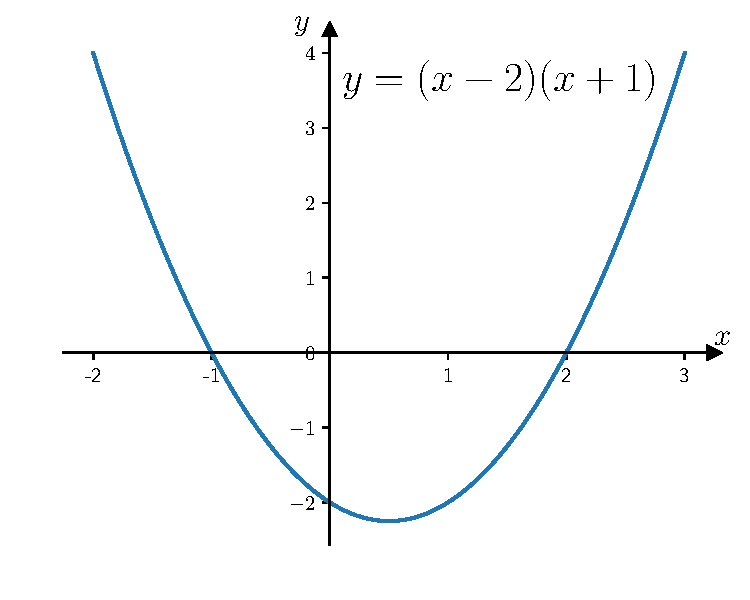
\includegraphics[width=0.5\textwidth]{figures/ch2_quadratic1.pdf} 
	  \caption{Quadratic $y=x^2 + x - 2$.} \label{fig:ch2_quadratic}
	\end{center}
\end{figure}

\noindent Or maybe you remember finding the intersection of two lines. E.g. for equations
\begin{align*}
y &= x +1 \\
y &= x^2 -2
\end{align*}
Visually we can intuit there will be 2 solutions
\begin{figure}[H]
	\begin{center}
	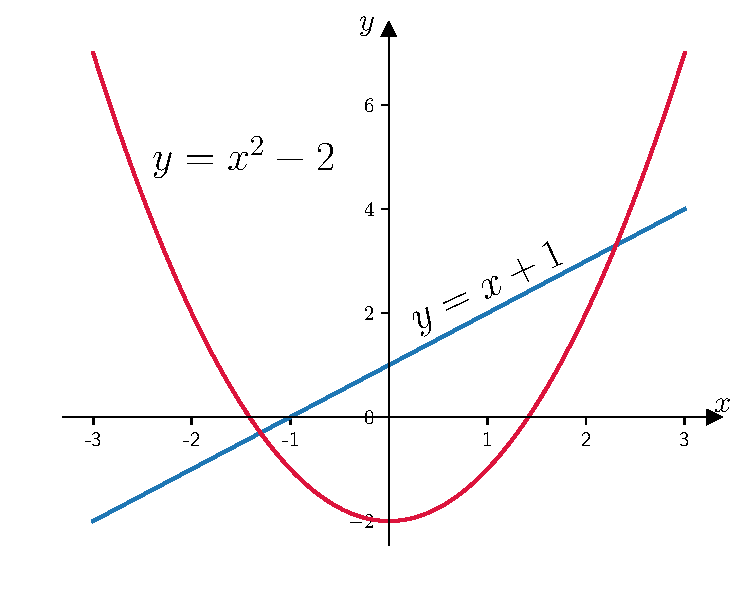
\includegraphics[width=0.5\textwidth]{figures/ch2_intersection2.pdf} 
	  \caption{Intersection of the lines $y=x + 1$ and $y= x^2 -2$.} \label{fig:ch2_intersection}
	\end{center}
\end{figure}

\noindent Letting the two equations be simultaneously true leads to the quadratic $x^2 - x - 3 = 0$ and you can use the quadratic formula again. 

As mentioned in the introduction, we may want to solve an equation with no analytic solution like $e^x = x+2$. This can be visualised as the intersection of the lines $y=e^x$ and $y=x+2$:
\begin{figure}[h]
	\begin{center}
	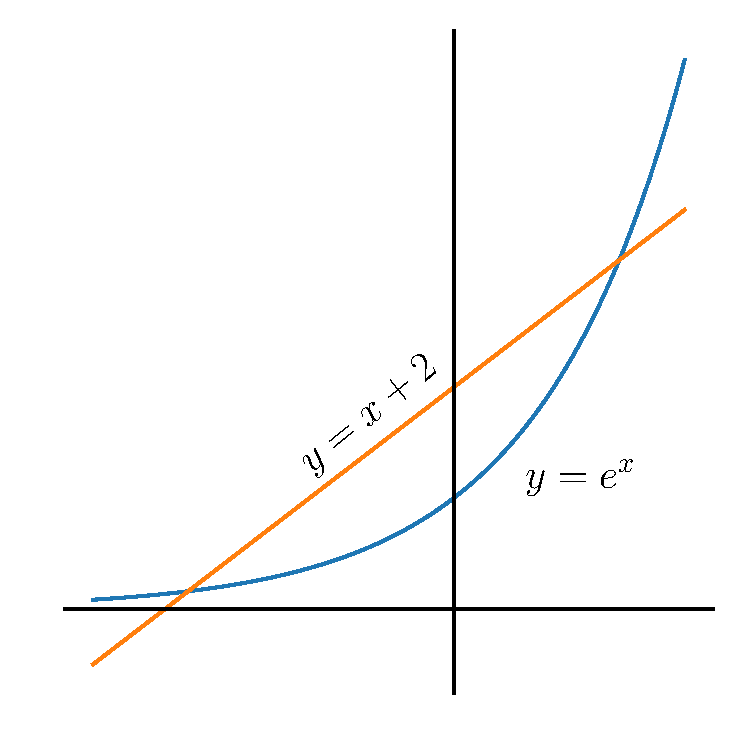
\includegraphics[width=0.5\textwidth]{figures/ch1_intersection1.pdf} 
	  \caption{Intersection of the lines $y=e^x$ and $y=x+2$.} \label{fig:ch2_intersection2}
	\end{center}
\end{figure}

\noindent We can rearrange the equation so that $e^x - x - 2 = 0$. Now the solutions ``zero'' this equation.

As a final example, consider the equation $\sin x = \cos x$. Visually we can intuit that there'll be infinite solutions:
\begin{figure}[H]
	\begin{center}
	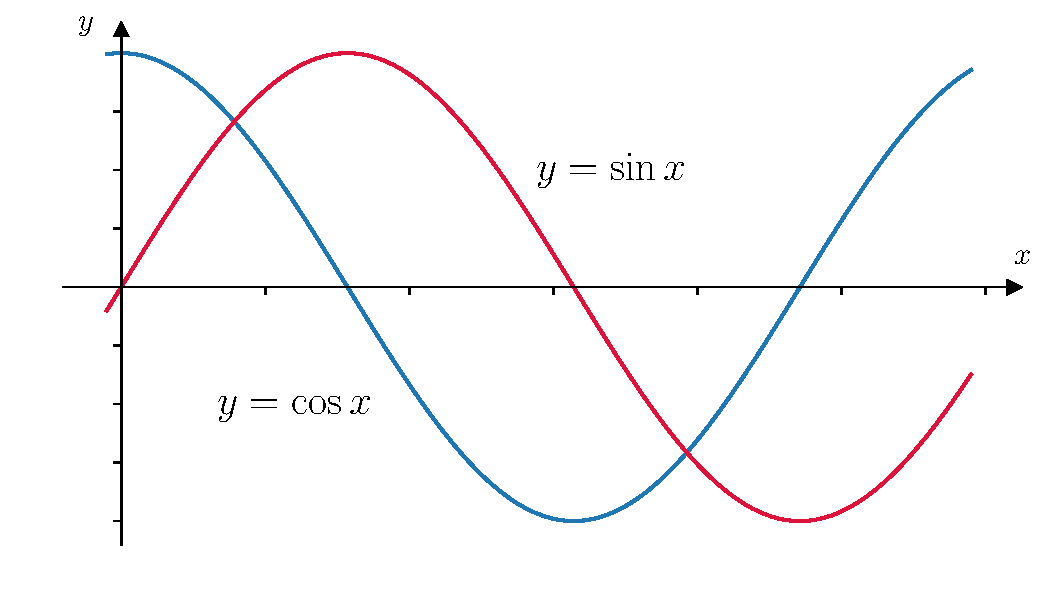
\includegraphics[width=0.5\textwidth]{figures/ch2_intersection3.pdf} 
	  \caption{Intersection of the lines $y=\sin x$ and $y=\cos x$.} \label{fig:ch2_intersection3}
	\end{center}
\end{figure}

\noindent We can also rearrange this equation so that the solutions zero a new equation $\sin x - \cos x = 0$.

The point of all these examples is that in many cases we will have equations of the form $f(x)=0$, even if we have to force equations to look that way. This is the form of the problems for this chapter, where we will develop techniques to find solutions, called the ``zeros of $f$'' or ``roots of $f(x)=0$''.


%%%%%%%%%%%%%%%%%%%%%%%%%%%%
%%%%%%%%%%%%%%%%%%%%%%%%%%%%
%%%%%%%%%%%%%%%%%%%%%%%%%%%%
%%%% BISECTION METHOD %%%%
%%%%%%%%%%%%%%%%%%%%%%%%%%%%
%%%%%%%%%%%%%%%%%%%%%%%%%%%%
%%%%%%%%%%%%%%%%%%%%%%%%%%%%
\section{Bisection}
This method is quite simple, we start by making an interval surrounding a root. Then we cut this interval in half. The root must exist in one of the halves. Focus on that half, and cut it further in half. Rinse and repeat. This procedure is sketched out in figure~\ref{fig:ch2_bisection_sketch}.
\begin{figure}[H]
	\begin{center}
	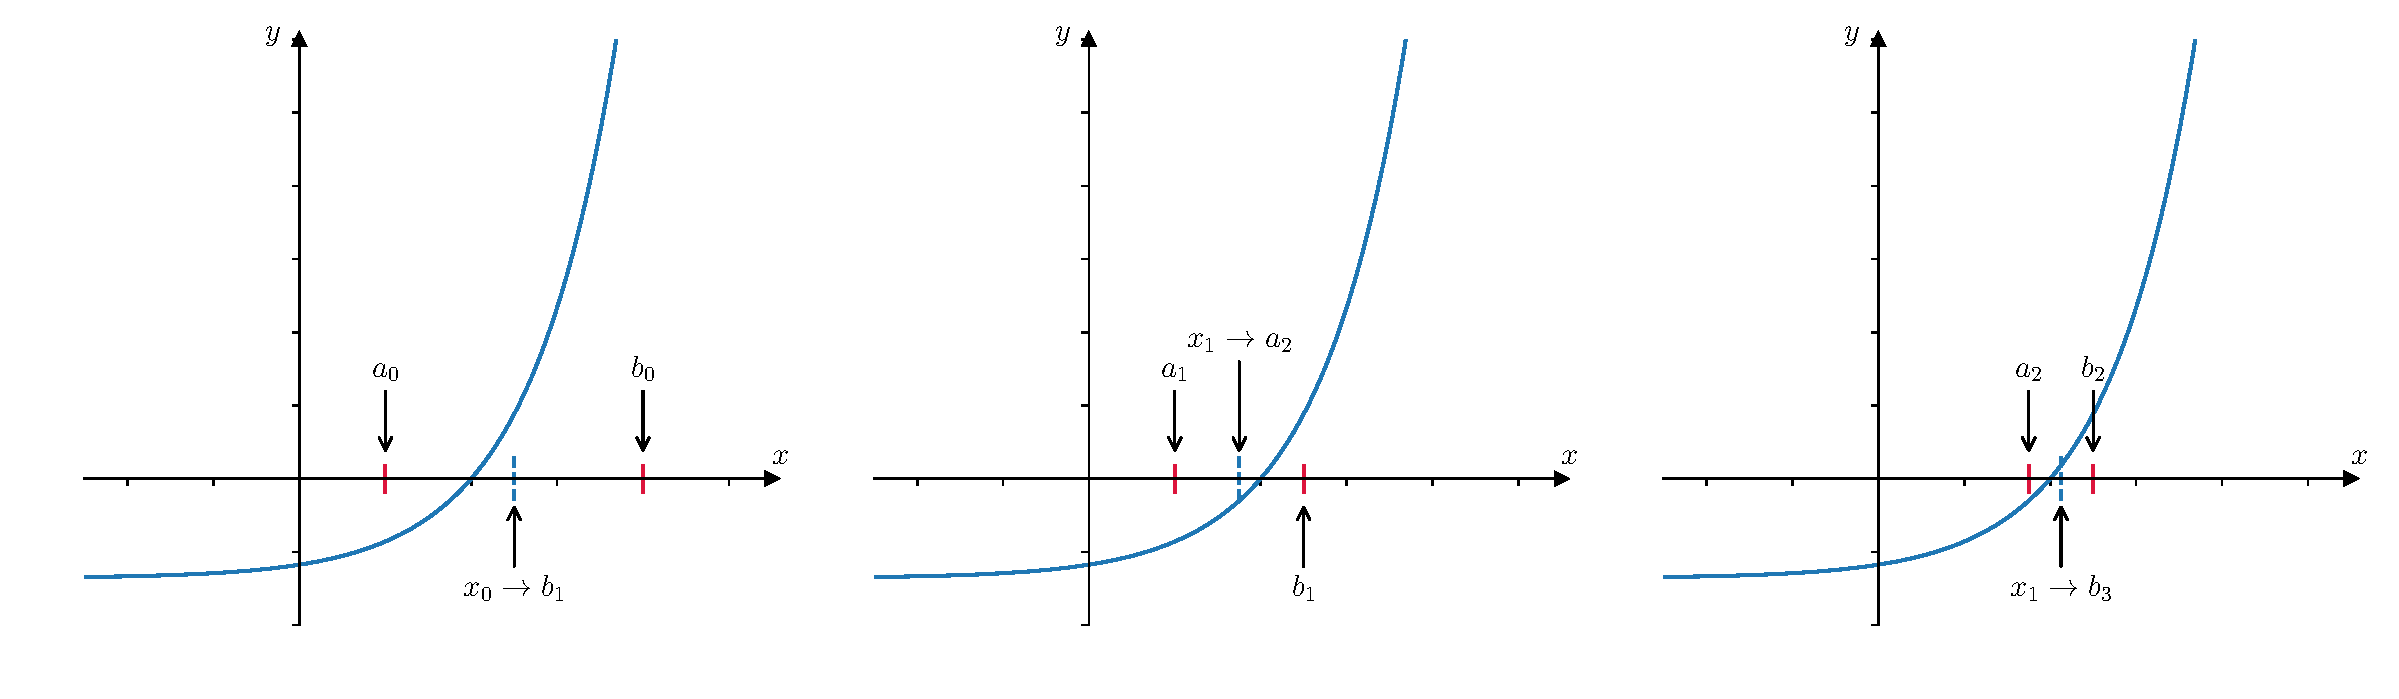
\includegraphics[width=\textwidth]{figures/ch2_bisection_intro.pdf} 
	  \caption{Sketch of 3 steps of the bisection method for rootfinding.} \label{fig:ch2_bisection_sketch}
	\end{center}
\end{figure}

\noindent This method is guaranteed to converge on \textit{a} root in the original interval, if one exists. So let's clearly define this algorithm. First we introduce a very useful theorem.

\theorem{INTERMEDIATE VALUE~}{}{Consider a function, $f(x)$, that is \textit{continuous} on an interval $[a,b]$. Choose any value $y$ such that $f(a) < y < f(b)$ or $f(b) < y < f(a)$. Then there exists an $x\in(a,b)$ such that $f(x)=y$.}\label{thm:ivf}

For our purposes, we want to use this theorem to find a root. Roots occur, by definition, when $y=0$. So we will want to find an $a$ and $b$ such that $f(a)<0$ and $f(b)>0$, or $f(a)>0$ and $f(b)<0$. We can condense both of these conditions (that the sign of $f$ is different at $a$ and $b$) into the relationship $f(a)f(b)<0$. If we have $f(a)f(b)<0$, then there exists an $x\in(a,b)$ such that $f(x)=0$. That is, there is a root in the interval (a,b).

\exemple{\upline}{
	Let $f(x)=\sin x - \cos x$. $\sin x$ and $\cos x$ are continuous functions for all $x$, and so $f$ is a continuous function over all reals. Let's search for an interval containing a root by looking at $x$ values that have clean answers with trigonometric functions.
	\begin{align*}
	& f(0) = -1
	& f(\pi) = 1
	\end{align*}
	So we have $f(0)f(\pi)=-1<0$. Hence by the intermediate value theorem, $f(x)=0$ has a root in $(0,\pi)$.
}{\downline}

Coming back to the bisection method, we can use the interval coming from the Intermediate Value Theorem as an initial interval, given we then know that a root is captured by it. So, the algorithm is as follows.

\vspace{0.2cm}
\noindent \fbox{\begin{minipage}{\linewidth}
\underline{\textbf{Bisection method for finding roots}}
\begin{enumerate}
	\item Given $a_0$ and $b_0$ such that $f(a_0)f(b_0)<0$, there is a root, $\xi \in (a_0,b_0)$.
	\item Define the midpoint
	\begin{align*}
	x_k = \frac{a_k + b_k}{2}
	\end{align*}
	\item If $f(x_k)f(a_k) < 0$, then the root $\xi \in (a_k,x_k)$. So let $a_{k+1}=a_k$ and $b_{k+1}=x_k$. Otherwise (that is, if $f(x_k)f(b_k) < 0$) the root $\xi \in (x_k,b_k)$ and we let $b_{k+1}=b_k$ and $a_{k+1}=x_k$.
\end{enumerate}
The midpoint $x_k$ is the series of values that will converge on the root, $x_k \to \xi$ as $k \to \infty$.
\end{minipage}}
\vspace{0.2cm}

\exemple{\upline}{
To use the bisection method to approximate $\sqrt{2}$, as promised in the previous chapter, we start with the desire to find the number $x=\sqrt{2}$. Then
\begin{align*}
& x^2  = 2 \\
& x^2  - 2 = 0
\end{align*}
and we have a rootfinding problem, where if we define $f(x) = x^2 -2$ then the number we want, $\sqrt{2}$, is a root of $f(x)=0$. Let's use the intermediate value theorem to justify a search interval:
\begin{itemize}
\item $f(1)=1-2=-1 < 0$
\item $f(2)=4-2=2 > 0$
\item $f(x)$ is continuous on $[1,2]$
\end{itemize}
therefore by the interediate value theorem there exists a root, $\xi$ (=$\sqrt{2}$), lying in the interval $(1,2)$. So we apply the bisection method with $a_0=1$ and $b_0=2$. Here are a few iterations
\begin{align*}
x_0 = \frac{1+2}{2} = 1.5  & \implies  f(x_0)f(a_0) = (1.5^2-2)(1^2-2) < 0 \\
& \implies \sqrt{2} \in (a_0,x_0) = (1,1.5) \\
& \implies a_1 = 1 \quad\text{and}\quad b_1 = 1.5 \\
%%
%%
x_1 = \frac{1+1.5}{2} = 1.25 & \implies f(x_1)f(a_1) = (1.25^2-2)(1.5^2-2) > 0 \\
& \implies \sqrt{2} \in (x_1,b_1) = (1.25,1.5) \\
& \implies a_2 = 1.25 \quad\text{and}\quad b_2 = 1.5 \\
%%
%%
x_2 = \frac{1.25+1.5}{2} = 1.375 & \implies f(x_2)f(a_2) = (1.25^2-2)(1.375^2-2) > 0 \\
& \implies \sqrt{2} \in (x_1,b_1) = (1.375,1.5) \\
& \implies a_2 = 1.375 \quad\text{and}\quad b_2 = 1.5
\end{align*}
and then $x_3=1.4375$ and so on.
}{\downline}

\subsubsection*{Convergence of the bisection method}
We know initially that the root, $\xi$, must be inside of the initial guesses for $a$ and $b$. At each step of the method the interval size is halved, so that the midpoint cannot be a wrong approximation of the root by more than half of the current interval size: 
\begin{align*}
|x_0 - \xi| &\leq \frac{|b_0 - a_0|}{2} \\
|x_1 - \xi| &\leq \frac{1}{2}|b_1 - a_1| = \frac{|b_0 - a_0|}{2^2} \\
|x_2 - \xi| &\leq \frac{1}{2}|b_2 - a_2| = \frac{|b_0 - a_0|}{2^3} \\
& \vdots
\end{align*}
You see the pattern, the error at iteration $i$, $\epsilon_i=|x_i - \xi|$, is limited by the original interval 
\begin{align*}
\epsilon_k \leq \frac{|b_0 - a_0|}{2^{k+1}}.
\end{align*}
The original interval is a fixed number, so it's pretty clear this error limits to zero as the iterations go to infinity
\begin{align*}
\lim_{k\to \infty} \epsilon_k = \lim_{k\to \infty} |x_k - \xi| = 0
\end{align*}
which proves that $x_i$ converges to the root.

It's natural to ask the inverse question "how many iterations must I perform in order to approximate the root to a given precision?" That is, given a required precision $\epsilon_g$, when can we be sure that the error $\epsilon_i$ is less than $\epsilon$. Well this will happen when
\begin{align*}
& \frac{|b_0 - a_0|}{2^{k+1}} \leq \epsilon_g \\
\implies & k \geq \frac{1}{\log 2}\log \left(\frac{|b_0 - a_0|}{\epsilon_g}\right) - 1.
\end{align*}

%%%%%%%%%%%%%%%%%%%%%%%%%%%%
%%%%%%%%%%%%%%%%%%%%%%%%%%%%
%%%%%%%%%%%%%%%%%%%%%%%%%%%%
%%%% FIXED-POINT ANALYSIS %%%%
%%%%%%%%%%%%%%%%%%%%%%%%%%%%
%%%%%%%%%%%%%%%%%%%%%%%%%%%%
%%%%%%%%%%%%%%%%%%%%%%%%%%%%
\section{Fixed-point analysis}

We can always rearrange the equation $f(x)=0$ into the form $x-g(x)=0$ for some newly defined function $g(x)$ that we'll call the \textit{auxiliary function}.

\exemple{\upline}{
	If we want to find the intersection points of $y=\sin x$ and $y=\cos x$, then we form 
	\begin{align*}
	\sin x - \cos x = 0
	\end{align*} 
	so that $f(x)=\sin x - \cos x$. To rearrange, simply force it into the new form by doing nothing (adding zero)
	\begin{align*}
	x - x + \sin x - \cos x = 0
	\end{align*}
	so that $g(x) = x - \sin x + \cos x$.
}{\downline}

The auxiliary function let's us define an iterative scheme
\begin{align*}
x_{k+1} = g(x_k).
\end{align*}
If there is a root of $f(x)=0$, the new form gives $\xi - g(\xi)=0 \implies \xi=g(\xi)$. Thinking this through, the function $g$ takes $\xi$ and gives you back the same number. For this reason $\xi$ is called a \textit{fixed point of $g$}. \textit{Fixed-points of auxiliary functions are roots of} $f(x)=0$, so it's worth studying them to solve the original problem we have. If the iteration scheme gives a sequence of values $x_1$, $x_2$, $x_3$, \dots that eventually land on $\xi$, then the sequence will remain unchanged, and the sequence will have converged on the root of $f(x)=0$. 

Now, how can we know if $\xi$ actually exists? To explore this question, consider the following theorem:

\theorem{BROUWER'S FIXED POINT~}{}{Suppose we have a function, $g(x)$, that is continuous on an interval $[a,b]$. If the function is bounded by that interval, that is $g(x) \in [a,b]$, for any $x \in [a,b]$, then we are guaranteed the existence of a fixed point in the interval. That is, there exists a $\xi  \in [a,b]$ such that $g(\xi)=\xi$.}

This theorem is easy enough to understand with a visual demonstration. Consider the function sketched in figure~\ref{fig:ch2_brouwer}. In this figure, can you put your pen on the left boundary of the dashed lined square, and draw a continuous line to the right boundary of the square (with $x\in[a,b]$ and $y\in[a,b]$), while staying inside the square and somehow avoid crossing the $y=x$ line? Of course you cannot. There will be \textit{at least} 1 intersection point. At each of the intersection points, $(\xi_1,g(\xi_1))$ , $(\xi_2,g(\xi_2))$, etc, you have the property that $\xi_k = g(\xi_k)$, because the intersection point is on both lines $y=x$ and $y=g(x)$ simultaneously.

\begin{figure}[H]
	\begin{center}
	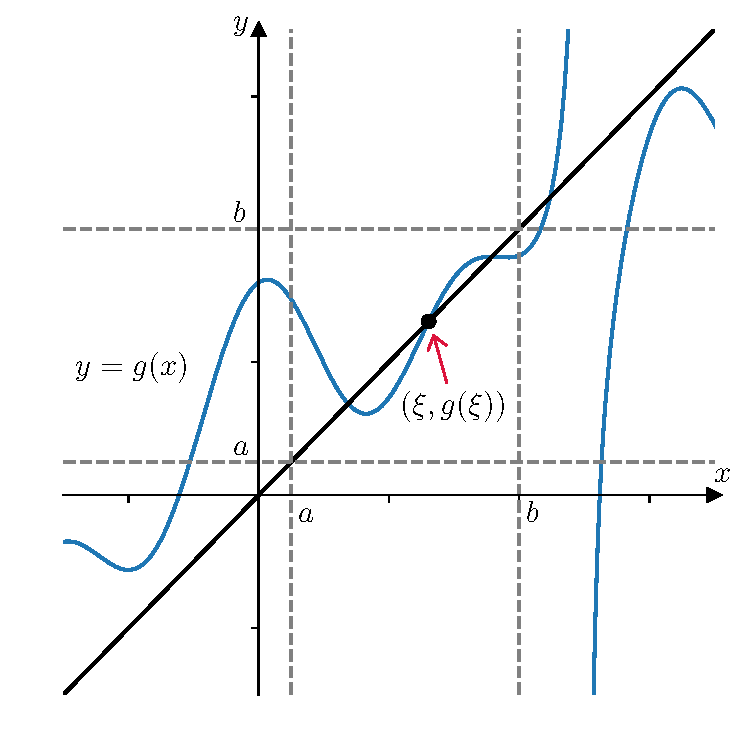
\includegraphics[width=0.7\linewidth]{figures/ch2_brouwer.pdf} 
	  \caption{Some arbitrary function, $g(x)$, satisfying the conditions of Brouwer's theorem. One point of intersection of $y=g(x)$ and $y=x$ is highlighted.} \label{fig:ch2_brouwer}
	\end{center}
\end{figure}

\exemple{\upline}{
	Let's consider the equation $e^x = x +2$. Solving this equation is equivalent to finding the roots of $f(x) = e^x - x - 2 = 0$. Instead of adding zero as we did when we were being abstract, let's just take the logorithm of both sides of the equation we want to solve:
	\begin{align*}
	x = \ln(x+2)
	\end{align*}
	so that if we define $g(x)=\ln(x+2)$ we have the form we want. Thus we define the iterative scheme
	\begin{align*}
	x_{k+1} = g(x_k) = \ln(x_k + 2).
	\end{align*}
	We showed earlier with the Intermediate Value Theorem that a root exists in the interval $[0,3]$. So let's make an initial guess $x_0=1$, and see where the iteration scheme takes us:
	\begin{align*}
	k  & \quad x_k \\
	0  & \quad 1 \\
	1  & \quad \ln(1 + 2) = 1.09861\dots \\
	2  & \quad \ln(1.09861\dots + 2) = 1.13095\dots \\
	3  & \quad \ln(1.13095\dots + 2) = 1.14134\dots \\
	   & \quad \vdots \\
	7  & \quad \ln(1.14604\dots + 2) = 1.14614\dots \\
	8  & \quad \ln(1.14614\dots + 2) = 1.14618\dots
	\end{align*}
	After the 8th iteration, the result has stopped changing to 4 decimal places, so that's a good enough place to stop. You can see that you can get more accuracy if you just keep iterating. This point, $\xi \sim 1.1462$ is clearly a fixed point of $g(x)$.
	
	Was this fixed point guaranteed by Brouwer's theorem? Let's consider the conditions of the theorem. We need the function to be continuous and enclosed in some square. Consider the interval in which we know there is a root $[0,3]$
	\begin{align*}
	& g(0) = \ln 2, \quad {\rm and} \quad 1 < 2 < e \quad \implies \quad 0 < \ln 2 < 1 < 3 \\
	& g(3) = \ln 5, \quad {\rm and} \quad 1 < 5 < e^3 \quad \implies \quad 0 < \ln 5 < 3.
	\end{align*}
	So we know the function starts between $[0,3]$ and ends between $[0,3]$. Now the next important fact is that the logarithm is a monotonically increasing function. So there can't be any weird oscillations in the function that let's the function leave the square (up or down) and come back to its end point in the square at $(3,\ln 5)$. This means a sketch of the function in the box looks like:
	\begin{figure}[H]
		\begin{center}
		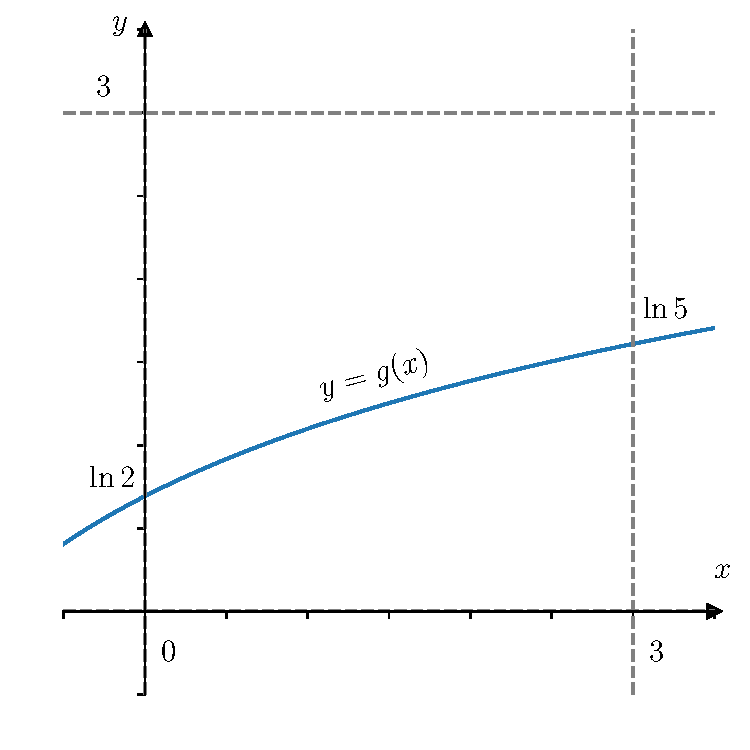
\includegraphics[width=0.5\linewidth]{figures/ch2_brouwer2.pdf} 
		  \caption{$g(x) = \ln(x+2)$ remaining in a square.} \label{fig:ch2_brouwer2}
		\end{center}
	\end{figure}
%	\noindent So we can say yes, Brouwer's theorem applies, and guarantees the existence of a fixed point $\xi \in [0,3]$.

	Now, the definition of an auxiliary function  is not unique. We could have rearranged the original equation differently
	\begin{align*}
	& e^x = x+ 2 \\
	& x = e^x - 2
	\end{align*}
	giving us a different auxiliary function $h(x) = e^x - 2$ so that $x=h(x)$. Now if we try to search in that same square, in the interval $[0,3]$
	\begin{align*}
	& h(0) = - 1 < 0 \\
	& h(3) = e^3 - 2 > 3.
	\end{align*}
	So we can say that it is \textit{not true} that $h(x)\in[0,3]$ for every $x\in[0,3]$. We can't satisfy one of the conditions in Brouwer's theorem, so we can't use it. However, if you sketch a graph of $y=h(x)$ and $y=x$, you will see the lines do in fact intersect in this square, and it definitely has a fixed-point in that region.
}{\downline}

Note the important lesson from that example, we proved with Brouwer's theorem that there is a fixed point of $g$, meaning that if we can find this fixed point we have the root of $f(x)=0$. We could not find a fixed point of $h(x)$. If we never defined $g(x)$, and we only thought of the second formulation, our failure to satisfy Brouwer's thorem \textit{does not} mean that there is no root of $f(x)=0$ in that interval. Only that we don't know one way or the other. So the lesson is to either choose a different interval to try to find a square in which your $g(x)$ does satisfy Brouwer's theorem, or to find a different rearrangement of $f(x)=0$ to define a $g(x)$ which works for us.

\subsection{Fixed-point iteration figures}
Let's now look at an important tool for visualising the fixed points: fixed-point iteration figures. The idea is simple:
\begin{enumerate}
	\item Graph the function $g(x)$;
	\item Graph the line $y=x$;
	\item For each iterate graph:
		\item[-] the vertical line from $(x,y)=(x_k,x_k)$ to $(x,y)=(x_k,g(x_k))$.
		\item[-] the horizontal line from $(x,y)=(x_k,g(x_k))$ to $(x,y)=(x_{k+1},x_{k+1})$ (i.e. until it intersects the $y=x$ lines).
\end{enumerate}
An example of these steps is sketched in figure~\ref{fig:ch2_fpfigures}, where we represent the different iterations for the scheme $x_k = \log(x_k + 2)$. 
\begin{figure}[H]
	\begin{center}
	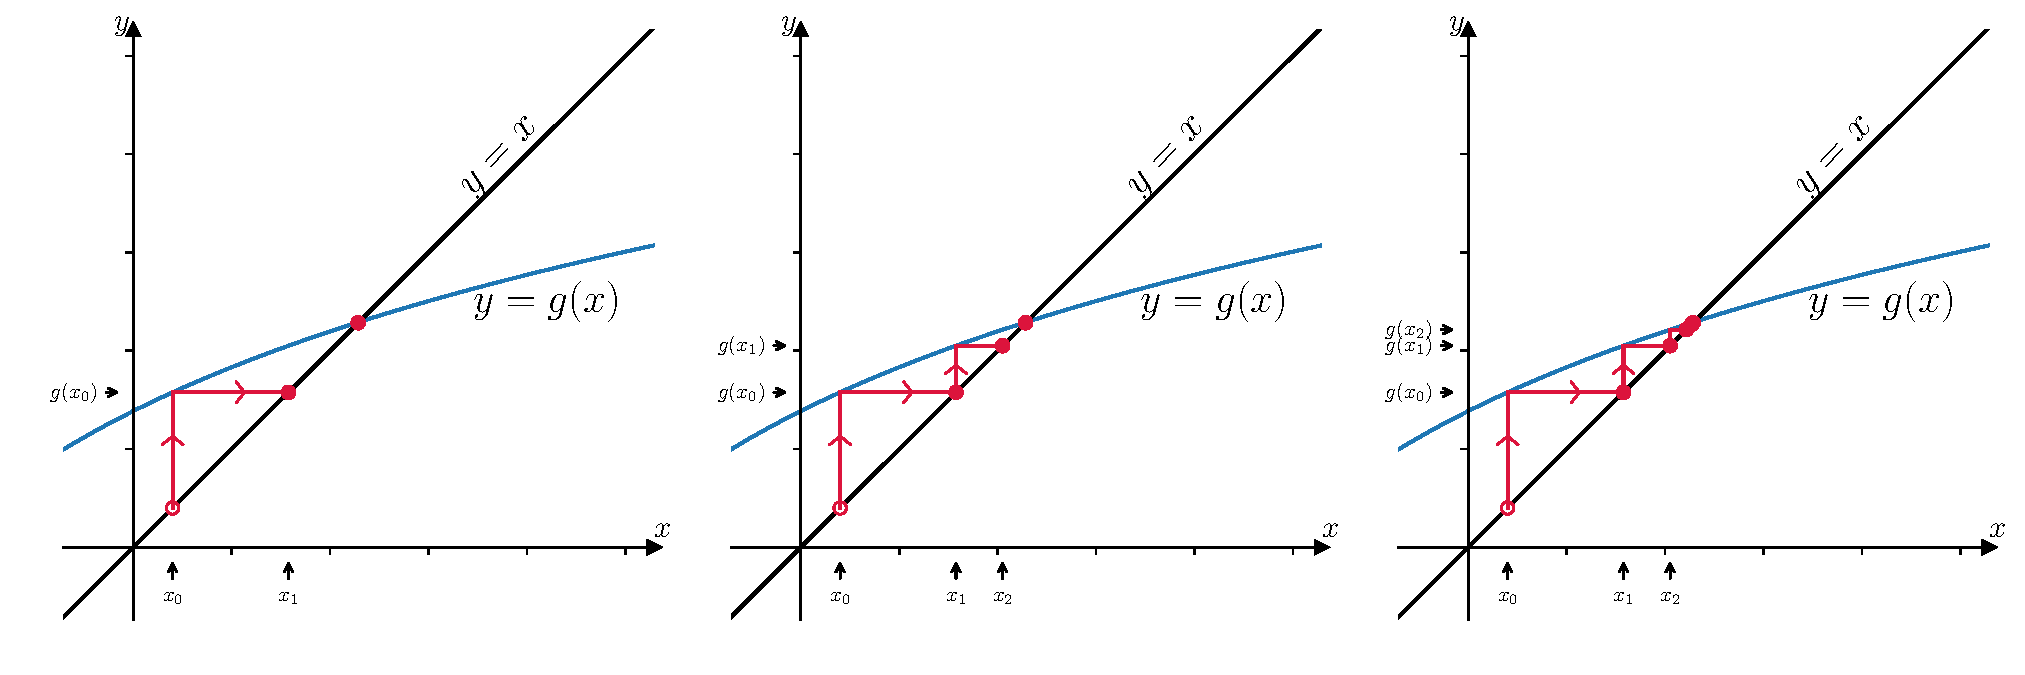
\includegraphics[width=\linewidth]{figures/ch2_fixedpoint.pdf} 
	  \caption{Fixed-point iteration figure step by step.} \label{fig:ch2_fpfigures}
	\end{center}
\end{figure}
\noindent These iteration figures help us understand why an iterative scheme converges on a fixed-point, which we will call a \textit{stable fixed-point}, or why it might diverge from a fixed-point, which we call an \textit{unstable fixed-point}.

\exemple{\upline}{
	Let's consider again the equation $e^x = x+2$, but we rearrange to give the iterative scheme that did not satisfy Brouwer's theorem in the previous example:
	\begin{align*}
	x = h(x) = e^x - 2.
	\end{align*}
	If you sketch the iteration figure accurately enough, shown in figure~\ref{fig:ch2_fpfigures2}, you will see that no matter how close to the intersection point you initially guess $x_0$ either on the left or right, your lines will be ``pushed'' away from it.
	\begin{figure}[H]
	\begin{center}
	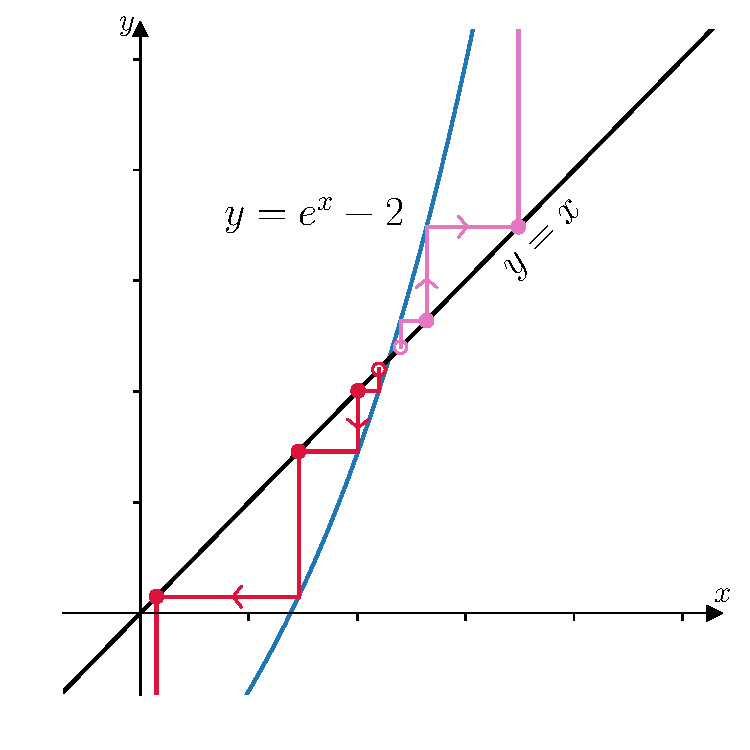
\includegraphics[width=0.5\linewidth]{figures/ch2_fixedpoint2.pdf} 
	  \caption{Fixed-point iteration figure for $h(x) = e^x - 2$.} \label{fig:ch2_fpfigures2}
	\end{center}
	\end{figure}
	\noindent So not only can we not use Brouwer's theorem (on the interval $[0,3]$) for this fixed-point, we also suspect that its fixed point is \textit{unstable}.
}{\downline}

\noindent These iteration figures can give you a rough expectation for whether a fixed-point will be stable or unstable. The next theorem clarifies this point.

\theorem{}{: FIXED-POINT STABILITY}{Consider an iteration scheme generated with the function $g(x)$ and one of its fixed-points $\xi$. $\xi$ is a \textit{stable fixed-point} if the gradient of nearby points is shallower than 1, i.e. $|g'(x\sim\xi)|<1$, and it is an \textit{unstable fixed-point} if the gradient of nearby points is steeper than $1$, i.e. $|g'(x\sim\xi)|>1$.}

This theorem is visually displayed in figure~\ref{fig:stability}. I think you can convince yourself that whenever you have a negative gradient the iterations will spiral, converging or diverging, around the fixed-point, and whenever you have a positive gradient the iterations will stay on one side, converging or diverging, of the fixed-point. Let's learn to use this stability theorem in practice with an example.

\begin{figure}
\centering
\begin{subfigure}[b]{.45\linewidth}
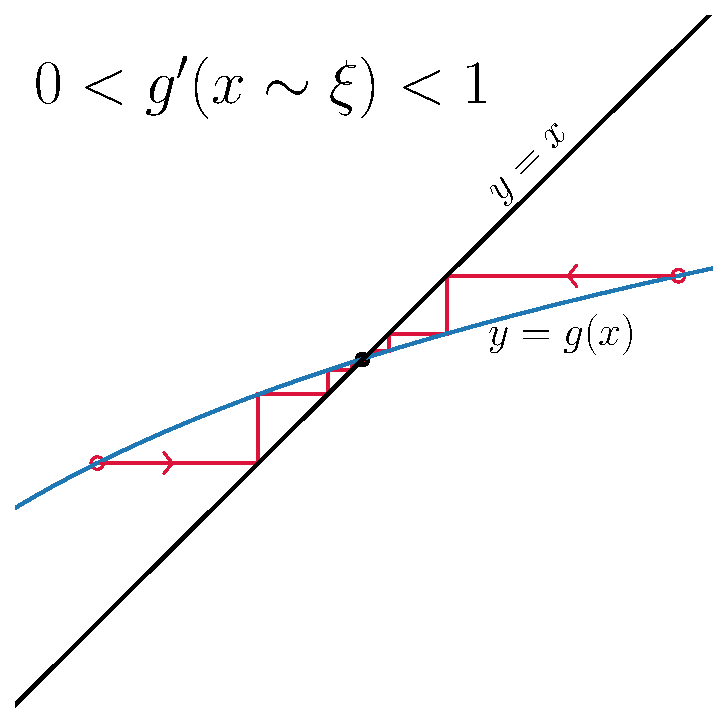
\includegraphics[width=\linewidth]{figures/ch2_stability1.pdf}
\caption{Stable point with $g'(x\sim \xi)>0$.}\label{fig:stable1}
\end{subfigure}
\begin{subfigure}[b]{.45\linewidth}
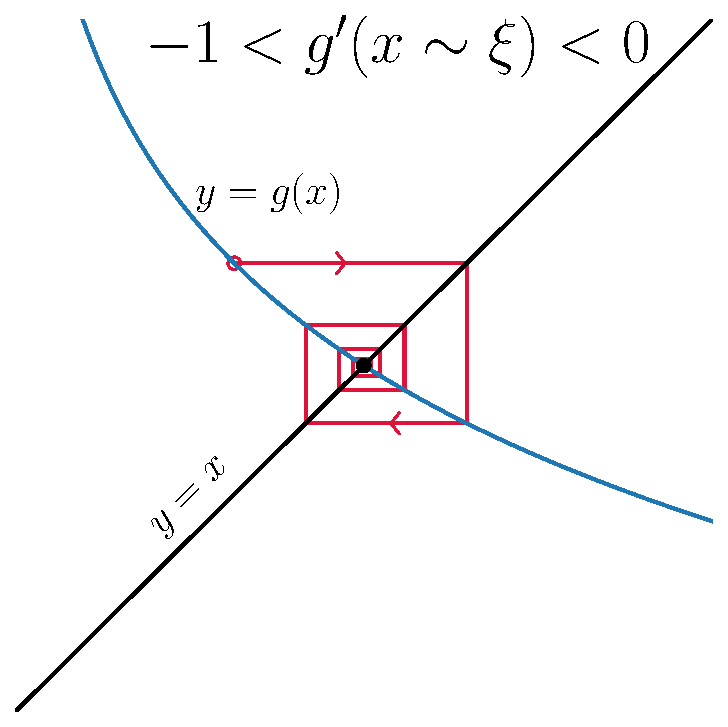
\includegraphics[width=\linewidth]{figures/ch2_stability2.pdf}
\caption{Stable point with $g'(x\sim \xi)<0$.}\label{fig:stable2}
\end{subfigure}

\begin{subfigure}[b]{.45\linewidth}
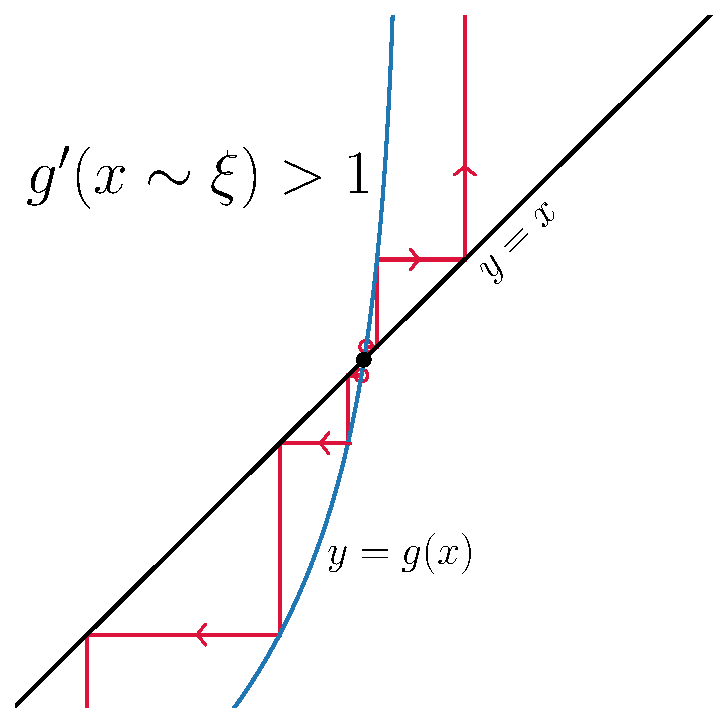
\includegraphics[width=\linewidth]{figures/ch2_stability3.pdf}
\caption{Unstable point with $g'(x\sim \xi)>0$.}\label{fig:stable3}
\end{subfigure}
\begin{subfigure}[b]{.45\linewidth}
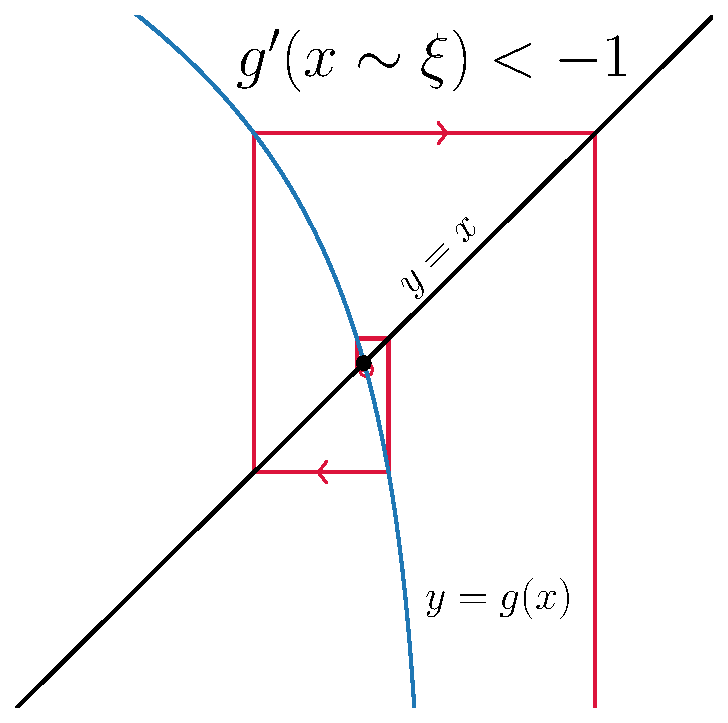
\includegraphics[width=\linewidth]{figures/ch2_stability4.pdf}
\caption{Unstable point with $g'(x\sim \xi)<0$.}\label{fig:stable4}
\end{subfigure}

\caption{Stable and unstable fixed points (filled black circles). Open red circles are initial guesses.}
\label{fig:stability}
\end{figure}

\exemple{\upline}
	{
	For the function $f(x) = e^x - x - 2$, if we define $g(x)=\ln(x+2)$, then fixed-points of $g$ are roots of $f(x)=0$. Let's consider the derivative near the fixed-point, that we previously proved must exist in the interval $[0,3]$.
	\begin{align*}
	g'(x) = \frac{1}{x+2}
	\end{align*}
	At the end points of the interval, the slopes are
	\begin{align*}
	& g'(0) = 1/2 < 1
	& g'(3) = 1/5 < 1.
	\end{align*}
	Additionally, $g'(x)$ is clearly a monotonically decreasing function. Therefore $g'(x) \in [1/5, 1/2]$ for all $x\in[0,3]$. Since we know the fixed-point is in this interval, we can confidently say $|g'(x)|<1$ near the point $\xi$, and hence it is a stable fixed-point.
	
	Now, there is a second fixed-point, we always knew that by looking at the sketch. We can localise it with the Intermediate Value Theorem. We have
	\begin{align*}
	&f(-1) = e^{-1} - 1 = \frac{1-e}{e} < 0 \\
	&f(-2) = e^{-2} > 0
	\end{align*}
	and hence there must be a root of $f(x)=0$ in the interval $[-2,-1]$, call it $\xi_-$. Remember, fixed-points of $g$ are roots of $f(x)=0$. This works both ways: roots of $f(x)=0$ are fixed-points of $g$. But, for this particular representation, $g(x)$ is not defined at $-2$. However, the gradient has a one-sided limiting value, so we can consider the stability by looking at these slopes
	\begin{align*}
	& g'(-1) = 1, {\rm but \, also \,} \lim_{x\to -1^-}g(x)=1^+\\
	& \lim_{x\to -2^+}g(x)=+\infty
	\end{align*}
	These two facts, along with the monotonic nature of $g'(x)$, tell us that $|g'(x)|>1$ at every point in the interval $[-2,-1]$. Therefore $\xi_-$ is an unstable fixed-point.
	}
{\downline}

This example proves fairly rigorously that $g(x)=\ln(x+2)$ provides us with an iterative scheme to converge on the positive root of $f(x)=0$, but cannot converge on the negative root. What if we look at the alternative iterative scheme we devised earlier by defining $h(x)=e^x - 2$?

\exemple{\upline}
	{	
	For the function $f(x) = e^x - x - 2$, if we define $h(x)=e^x - 2$, then fixed-points of $h$ are roots of $f(x)=0$. We know a fixed-point, $\xi_-$, exists in $[-2,-1]$, and the slopes at the end points are
	\begin{align*}
	& h'(x) = e^x \\
	& h'(-2) = e^{-2} < 1 \\
	& h'(-1) = e^{-1} < 1.
	\end{align*}
	$e^x$ is monotonically increasing, so the slopes must always be less than 1 in the interval. Hence $|h'(x)|<1$ near the point $\xi_-$ and the fixed-point is stable. Thus the iterative scheme
	\begin{align*}
	x_k = h(x_k) = e^{x_k} - 2
	\end{align*}
	will converge on $\xi_-$ given an initial guess that is close enough. So we can find this root, let's guess $x_0=-1$:
	\begin{align*}
	k  & \quad x_k \\
	0  & \quad -1 \\
	1  & \quad  e^{-1} - 2 = -1.63212\dots \\
	2  & \quad  e^{-1.63212\dots} - 2 = -1.80449\dots \\
	3  & \quad  e^{-1.80449\dots} - 2 = -1.83544\dots \\
	   & \quad \vdots \\
	7  & \quad  e^{-1.84138\dots} - 2 = -1.84140\dots \\
	8  & \quad  e^{-1.84140\dots} - 2 = -1.84141\dots \\
	\end{align*}
	and so we see that the iterations of $x_k$ get closer and closer to a number, which has stopped changing in the 4th decimal place by the 8th iteration. The second root of $f(x)=0$ is thus $\xi_- \sim -1.8414$.
	
	So we see that this alternative formulation of the iterative scheme let's us converge on the negative root. What does it do near the positive root? Looking at the slopes for the interval $[1,3]$ (remember we know the fixed-point is at $\xi \sim 1.1462$)
	\begin{align*}
	& h'(1) = e^{1} > 1 \\
	& h'(3) = e^{3} > 1.
	\end{align*}
	So with the monotonic fact, the slope must always be too steep near this fixed point. Hence it is unstable.
	}
{\downline}

These two examples show that the stability of a fixed-point is a property of the auxiliary function, and not of the original function $f(x)$. 



%%%%%%%%%%%%%%%%%%%%%%%%%%%%
%%%%%%%%%%%%%%%%%%%%%%%%%%%%
%%%%%%%%%%%%%%%%%%%%%%%%%%%%
%%%% NEWTON'S METHOD %%%%
%%%%%%%%%%%%%%%%%%%%%%%%%%%%
%%%%%%%%%%%%%%%%%%%%%%%%%%%%
%%%%%%%%%%%%%%%%%%%%%%%%%%%%
\section{Newton-Raphson methods}

Start with the general equation of an iterative scheme, $x = g(x)$, which is supposed to find roots of $f(x) = 0$. Previously we arbitrarily defined $g(x)$ by manipulation of $f(x)$. Here we will be more systematic.

Let $g(x) = x - \phi(x) f(x)$ for \textit{any} function $\phi(x)$ as long as $0 < |\phi(x)| < \infty$ in an interval $[a,b]$ containing a root, call it $\xi$. In other words, $\phi(x)$ must be continuous in this interval. Since $\xi$ is a root, we have $f(\xi)=0$ and hence
\begin{align*}
g(\xi) = \xi - \phi(\xi)\cancel{f(\xi)} = \xi.
\end{align*}
This shows that any zero of $f$ is a fixed point of this $g$ auxiliary function. For the other direction
\begin{align*}
g(\xi) = \xi \quad &\implies\quad \xi - \phi(\xi)f(\xi) = \xi\\
&\implies \phi(\xi)f(\xi) = 0
\end{align*}
and since $\phi(\xi)\neq 0$ in this interval, we must have $f(\xi)=0$. So any fixed point of $g$ is also a zero of $f$. Thus $x_{k+1} = g(x_k) = x_k - \phi(x_k) f(x_k)$ defines an iterative scheme for finding roots of $f(x)=0$. Different choices of the function $\phi(x)$ give different methods. We will highlight some of these choices in increasing order of complexity.

\subsection{Chord method}
In the simplest method we simply choose a constant function $\phi(x)=\alpha \neq 0$, giving the auxiliary function
\begin{align*}
\boxed{g(x) = x - \alpha f(x) \quad \text{or} \quad x_{k+1} = x_k - \alpha f(x_k) \quad (\text{Chord method})}
\end{align*}
This iterative scheme can be rearranged to give the constant
\begin{align*}
\alpha =  \frac{x_k - x_{k+1}}{f(x_k)} \implies \frac{1}{\alpha} = \frac{f(x_k)-0}{x_k - x_{k+1}}
\end{align*}
where we recognise that $1/\alpha$ is therefore the slope of a straight line with rise $f(x_k)$ and run $x_k - x_{k+1}$. This gives the following picture
\begin{figure}[H]
\begin{center}
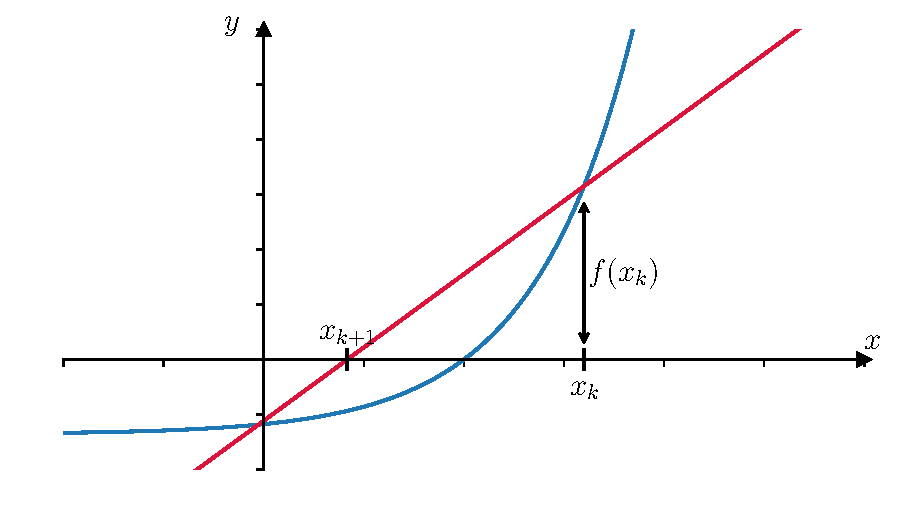
\includegraphics[width=0.5\linewidth]{figures/ch2_chord1.pdf}  \label{fig:ch2_chord1}
\end{center}
\end{figure}
\noindent showing that the iteration scheme gives an $x$-axis intercept as the next approximation of the root. If we take multiple iterations, and two different values of $\alpha$, we see the following
\begin{figure}[H]
\begin{center}
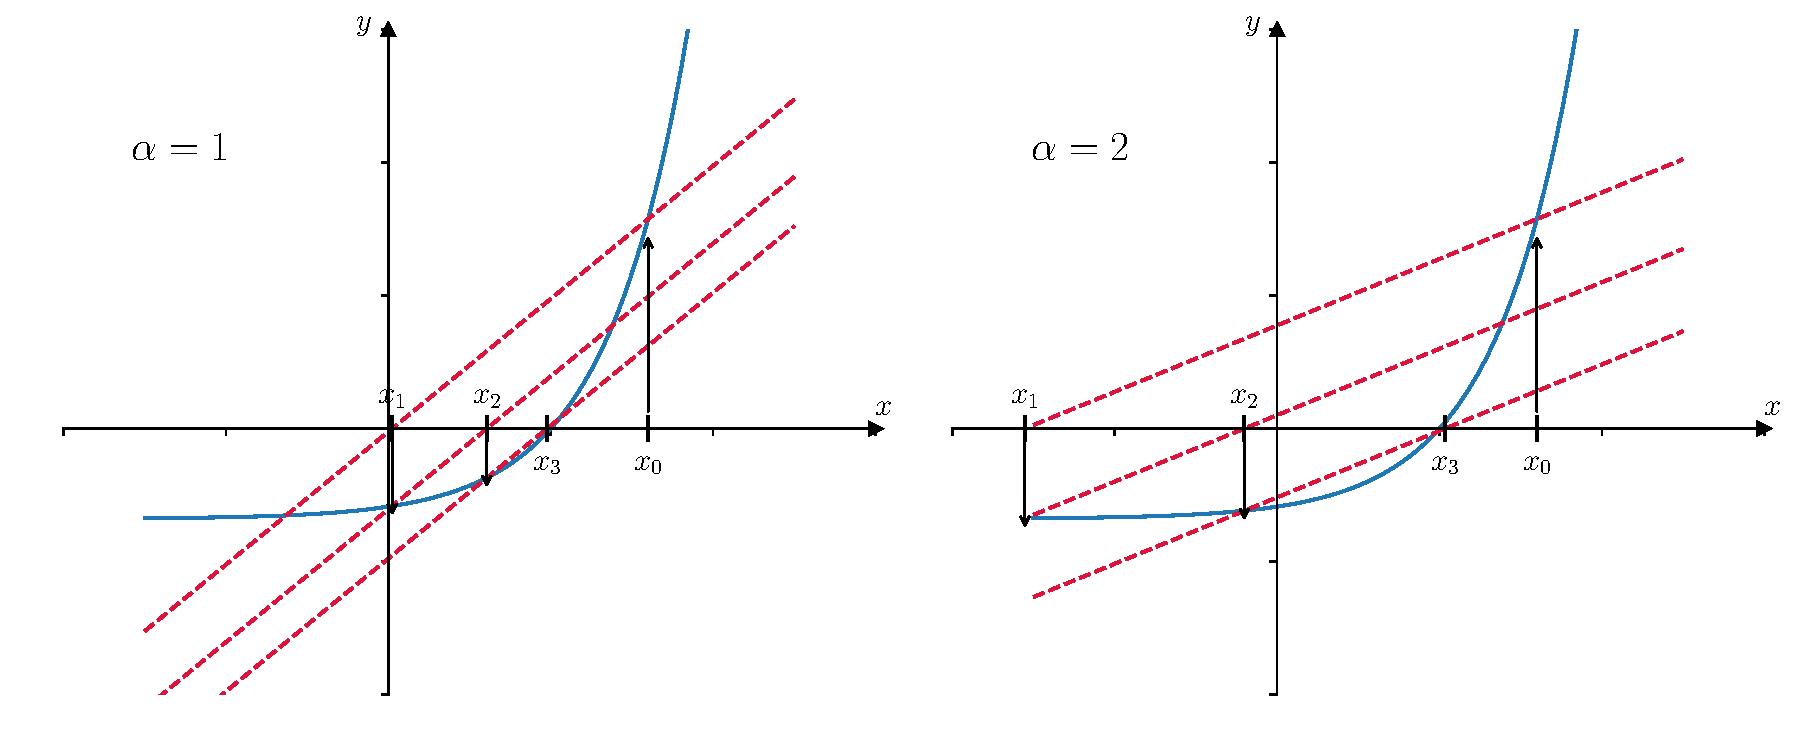
\includegraphics[width=0.9\linewidth]{figures/ch2_chord3.pdf}  \label{fig:ch2_chord2}
\end{center}
\end{figure}
\noindent showing that the choice of $\alpha$ fixes a slope that projects from the function (blue curve) at the previous approximation of the root, $(x_k,f(x_k))$, to the $x$-axis $(x_{k+1},0)$. This inspires the question, what is the optimal slope to choose in order to converge faster on the root? (Not to mention, do we know that this method will converge in all cases?)

\subsection{Newton's method}

Recall from the fixed-point analysis that the stability of a fixed point depends on the derivative of the auxiliary function near the fixed point. There was a criterion that required $|g'(x)|  < 1$ for $x$ near the root. Well it's not hard to see that if this derivative is 0 we will have immediate convergence.

So take the Chord method, $x_{k+1}=g(x_k) = x_{k} - \alpha f(x_{k})$ but imagine changing the constant $\alpha$ at every iteration, forcing $g'(x_k)$ to be zero. This would give
\begin{align*}
1 - \alpha_k f'(x_{k})=0 \quad\implies\quad \alpha_k = \frac{1}{f'(x_{k})}
\end{align*}
which gives us a new iteration scheme
\begin{align*}
\boxed{x_{k+1} = x_{k} - \frac{ f(x_{k})}{f'(x_{k})} \quad (\text{Newton's method})}
\end{align*}
\begin{figure}[H]
\begin{center}
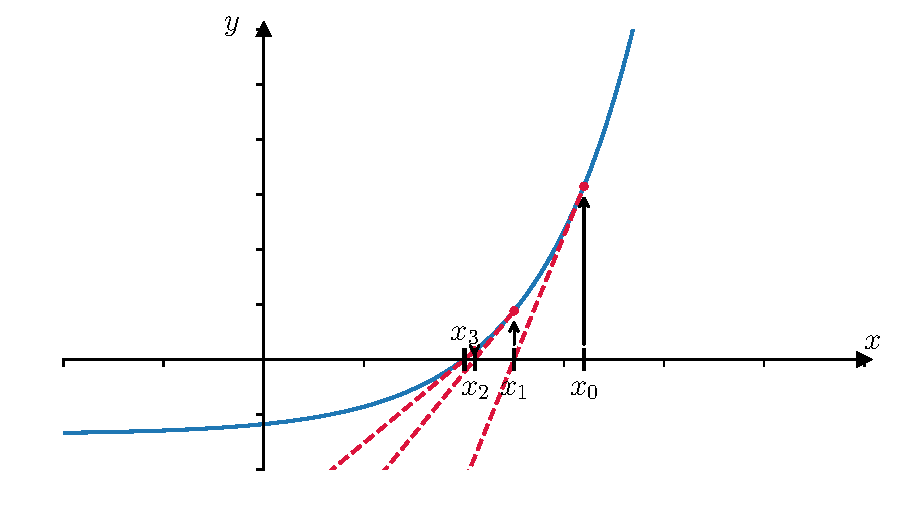
\includegraphics[width=0.7\linewidth]{figures/ch2_newton2.pdf}  \label{fig:ch2_newton2}
\end{center}
\end{figure}

Newton's method is a powerful method for finding roots, usually reaching a given precision faster than the chord method due to it's adaptive nature. There is, however, a problem. What happens if an iteration happens to land at a stationary point of the function $f(x_k)$? At this point the slope is zero, $f'(x_k)=0$, and the next iteration is not defined. This situation is shown below
\begin{figure}[H]
\begin{center}
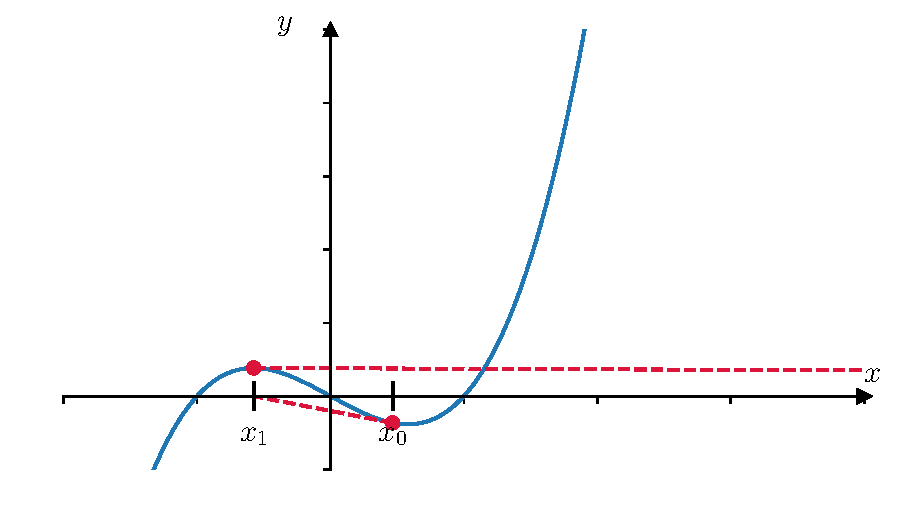
\includegraphics[width=0.7\linewidth]{figures/ch2_newton3.pdf}  \label{fig:ch2_newton3}
\end{center}
\end{figure}



\exemple{\upline}
	{	
	Let's use Newton's method to find some intersection points for $\sin x = \cos x$. We thus define $f(x) = \sin x - \cos x$ so that the intersection points are now zeros of this function $f$ and we have forced a rootfinding problem. We need the derivative $f'(x) = \cos x + \sin x$ and the iterative scheme is therefore
	\begin{align*}
	x_{k+1} = x_k - \frac{\sin x_k - \cos x_k}{\cos x_k + \sin x_k}
	\end{align*}
	This scheme is in fact well defined for any $x\in\mathbb{R}$ since $sin x - cos x$ is never zero. If we make an initial guess at $x_0=1.5$, the result stabilises in the 4th decimal place after just 4 iterations on $x_4 = 0.7854$. Whereas if we start at $x_0=2$ the result stabilises, to 4 decimal places, after 6 iterations, and at a different root! These iterations are shown in the following table:	
	\begin{table}[H]
	\begin{center}
	\begin{tabular}{ccr}
	$k$  &  $x_k$  &  $x_k$ \\ \hline
	0  &  $1.5000$  &  $2.0000$ \\
	1  &  $0.6324$  &  $-0.6877$  \\
	2  &  $0.7866$  &  $9.5160$  \\
	3  &  $0.7854$  &  $10.3484$  \\
	4  &  $0.7854$  &  $10.2092$   \\
	5  &  $0.7854$  &  $10.2102$   \\
	6  &  $0.7854$  &  $10.2102$ 
	\end{tabular}
	\end{center}
	\end{table}
	and on a figure 
	\begin{figure}[H]
	\begin{center}
	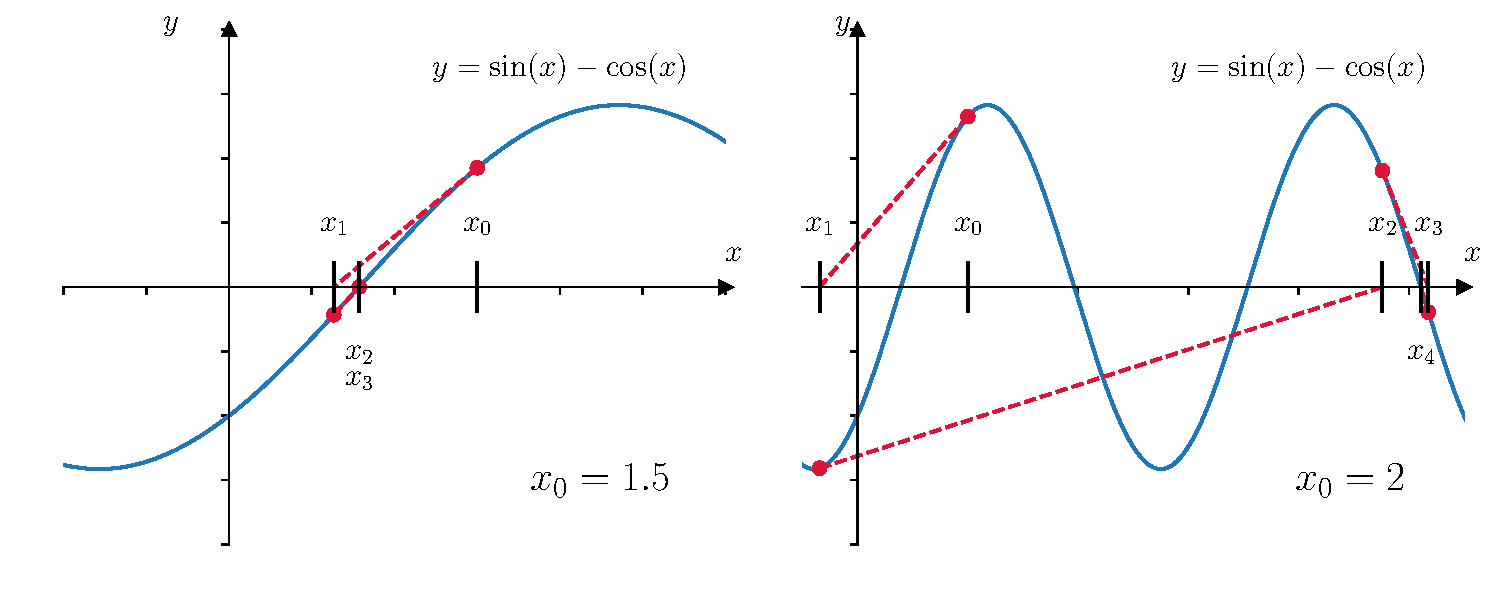
\includegraphics[width=\linewidth]{figures/ch2_newton4.pdf}  \label{fig:ch2_newton4}
	\end{center}
	\end{figure}
	we can see how wildly the second initial guess jumps around.
	}
{\downline}


\subsection{Secant method}

Newton's method requires the calculation of a derivative $f'(x)$ to define an iterative scheme. If the derivative is analytic (for example $(\cos x)' = \sin x$) then this is easy. But there can be situations where $f$ is not known analytically, and so neither is its derivative. In the secant method we follow Newton's method but make an approximation for the derivative:

\begin{align*}
\boxed{x_{k+1} = x_{k} - \frac{x_k - x_{k-1}}{f(x_{k}) - f(x_{k-1})}  f(x_{k}) \quad (\text{Secant method})}
\end{align*}

We have approximated the derivate with
\begin{align*}
f'(x_k) \sim \frac{f(x_{k}) - f(x_{k-1})}{x_k - x_{k-1}}
\end{align*}
which will be justified in a later chapter. What you can recognise is that to calculated $x_{k+1}$ we need the previous two iterations. So we must start with two initial guesses. The method is illustrated below for 3 iterations.
\begin{figure}[H]
\begin{center}
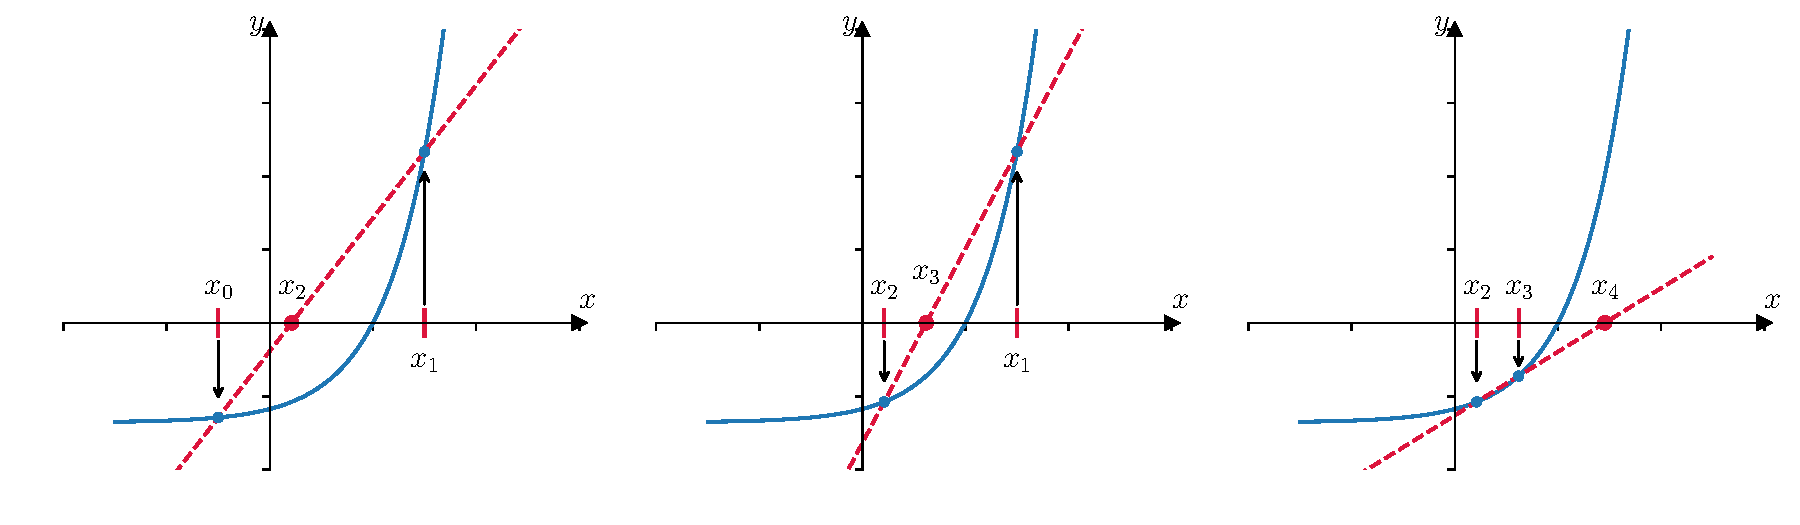
\includegraphics[width=\linewidth]{figures/ch2_secant1.pdf}  \label{fig:ch2_secant1}
\end{center}
\end{figure}

\noindent Notice that the approximation doesn't always stay on the same side of the function (blue curve), and in fact $x_4$ is even further away from the root than $x_3$. Sometimes it may take several iterations to settle down.


%%%%%%%%%%%%%%%%%%%%%%%%%%%%
%%%%%%%%%%%%%%%%%%%%%%%%%%%%
%%%%%%%%%%%%%%%%%%%%%%%%%%%%
%%%% Comparison %%%%
%%%%%%%%%%%%%%%%%%%%%%%%%%%%
%%%%%%%%%%%%%%%%%%%%%%%%%%%%
%%%%%%%%%%%%%%%%%%%%%%%%%%%%
\section{Comparison of methods}

For any of the methods we have studied, consider the error at each iteration $\epsilon_k = |x_k - \xi|$ where $\xi$ is a root. If we find that the following limit gives a constant 
\begin{align*}
\lim_{k\to\infty} \frac{\epsilon_{k+1}}{\epsilon_k^p} = C
\end{align*}
for some constant $C>0$, then we say the method has \textit{order of convergence} $p$. Note that $p$ is not forced to be an integer. This characterizes a rate of convergence and therefore lets us compare which method will reach a certain precision faster than another.

\subsection*{Bisection method}
We showed that the error in the bisection method is bounded
\begin{align*}
\epsilon_k \leq \frac{|b_0 - a_0|}{2^k}.
\end{align*}

\begin{align*}
\lim_{k\to\infty}\left( \dfrac{\frac{|b_0 - a_0|}{2^{k+1}}}{\frac{|b_0 - a_0|}{2^k}} \right)
=
\lim_{k\to\infty} \frac{1}{2}
=
\frac{1}{2}
\end{align*}


\subsection*{Newton method}
\subsection*{Secant method}


%%%%%%%%%%%%%%%%%%%%%%%%%%%%
%%%%%%%%%%%%%%%%%%%%%%%%%%%%
%%%%%%%%%%%%%%%%%%%%%%%%%%%%
%%%% Exercises %%%%
%%%%%%%%%%%%%%%%%%%%%%%%%%%%
%%%%%%%%%%%%%%%%%%%%%%%%%%%%
%%%%%%%%%%%%%%%%%%%%%%%%%%%%
\exercises{
\section{Exercises}

\exercice{Finding the intersection of $2\sin x=x$}
\begin{enumerate}[label=\alph*)]
	\item Sketch a graph of $y=2\sin x$ and $y=x$ in the domain $[-2\pi,2\pi]$. 
	
	\item Write a function $f(x)$ that has roots corresponding to the solutions of $2\sin x=x$.
	
	\item Use the Intermediate Value Theorem and the graph to find \textit{the number} of roots of $f(x)$, and give intervals surrounding them.
	
	\item Use the bisection algorithm to solve $2\sin x=x$ for as many iterations as needed       until the solution stops changing its first 4 decimal places. Do this for each       solution of $2\sin x=x$ that you found in part c.
	
	\item Define a function $g(x)$ so that we have an iterative scheme: $x_{k+1} = g(x_k)$ with fixed points at the roots of $f(x)$.
	
	\item Make a rough iteration figure exploring initial guesses $x_0$ and their subsequent      iterates using the iteration scheme of part e. Are there any unstable fixed-points? What value does $x_k$ converge to for initial $x_0$ where $\sin(x_0)>0$? What about initial $x_0$ where $\sin(x_0)<0$?
\end{enumerate}



\exercice{Finding the intersection of $\sin x=\cos x$}
\begin{enumerate}[label=\alph*)]
	\item Sketch a graph of $y=\sin x$ and $y=\cos x$ in the domain $[0,2\pi]$. 
	
	\item Write a function $f(x)$ that has roots corresponding to the solutions of $\sin x=\cos x$.
	
	\item Use the Intermediate Value Theorem and the graph to find \textit{the number} of roots of $f(x)$, and give intervals surrounding them.
	
	\item Use the bisection algorithm to solve $\sin x=x$ for as many iterations as needed       until the solution stops changing its first 4 decimal places. Do this for each       solution of $\sin x=\cos x$ that you found in part c.
\end{enumerate}



\exercice{Fixed-point analysis $g(x)=x(x^2-1)$}
\begin{enumerate}[label=\alph*)]
	\item How many fixed points, $\xi_k$, of $g(x)$ are there?
	
	\item Sketch a graph of $y=g(x)$ and $y=x$. Make rough iteration figures at different initial guesses $x_0$ on each side of the fixed points. Which fixed point(s) do you expect to be stable?
	
	\item Use the stability criterion on $|g(\xi_k)|$ to make a stability analysis of the fixed points.
\end{enumerate}



\exercice{Fixed-point analysis $f(x)=2e^{-x} + x - 2$}
\begin{enumerate}[label=\alph*)]
	\item Find 2 functions $g(x)$ for which the $x=g(x)$ has the same solutions as zeros of $f(x)$.
	
	\item Sketch separate graphs of the previous functions, as well as $y=2e^x$ and $y=2-x$ to get an intuition on the location of the roots or fixed points.
	
	\item Can you use Brouwer's theorem to guarantee the existence of any fixed points for either of the functions defined in part a?
	
	\item Make a stability analysis of the fixed points for both functions.
	
	\item For any stable fixed points, use the iterative scheme $x_{k+1}=g(x_k)$ for 5 iterations.
\end{enumerate}



\exercice{The intersection of $e^x=\cos x + 1$}
\begin{enumerate}[label=\alph*)]
	\item Sketch a graph of $y=e^x$ and $y=\cos x + 1$ in the domain $[-4\pi,4\pi]$. 
	
	\item Write a function $f(x)$ that has roots corresponding to the solutions of $e^x=\cos x + 1$.
	
	\item From the graph, how many positive roots and how many negative roots of $f(x)$ will there be?
	
	\item Use the Intermediate Value Theorem and the graph to prove there is a root of $f(x)$, for $x>0$.
	
	\item Use Netwon's method to propose an iterative scheme to find the roots of $f(x)$. Use this iterative scheme starting with $x_0=0$ to make a table of estimates $x_k$ for $k=0,1,\dots ,4$.
	
	\item Show that the function $g(x)=\log(\cos x + 1)$ gives an iterative scheme $x_{k+1} = g(x_k)$ with fixed points equal to the roots of $f(x)$. Determine a second function $h(x)$ which also satisfies these properties.
	
	\item Sketch a graph of $y=g(x)$ and $y=x$ in the domain $[-\pi,\pi]$. 
	
	\item Make a rough iteration figure exploring initial guesses x0 and their subsequent iterates using the iteration scheme with $g(x)$ of part f. Which fixed point(s) do you expect to be stable?
	
	\item Use the stability criterion on $|g(\xi_k)|$ to make a stability analysis of the fixed points $\xi_k \in [-\pi,\pi]$.
\end{enumerate}



\exercice{Fixed-point analysis $\log(x+2)=x^2$}
\begin{enumerate}[label=\alph*)]
	\item Sketch a graph of $y=\log(x+2)$ and $y=x^2$. 
	
	\item Write a function $f(x)$ that has roots corresponding to the solutions of $\log(x+2)=x^2$.
	
	\item From the graph, how many roots of $f(x)$ will there be?
	
	\item Use the Intermediate Value Theorem and the graph to locate the roots of $f(x)$.
	
	\item Use the Secant method to propose an iterative scheme to find the roots of $f(x)$. Use this iterative scheme twice, starting with $x_0=1$ and $x_1=2$ and then again with $x'_0=-1$ and $x_1=-1.5$ to make a table of estimates of $x_k$ and $x'_k$ until $k=4$.
	
	\item Show that the functions $g_1(x)=\exp(x^2)-2$ and $g_2(x)=( \log(x+2) )1/2$ give iterative schemes $x_{k+1} = g_i(x_k)$ with fixed points equal to the roots of $f(x)$.
	
	\item Sketch a graph of $y=g_1(x)$ and $y=x$. Sketch another graph of $y=g_2(x)$ and $y=x$. Can you use Brouwer's theorem to guarantee the existance of any fixed points for either $g_1(x)$ or $g_2(x)$?
	
	\item Make a rough iteration figure exploring initial guesses $x_0$ and their subsequent iterates using the iteration scheme with $g(x)$ of part f. Which fixed point(s) do you expect to be stable?
	
	\item Use the stability criterion on $|g_1(\xi_k)|$ and $|g_2(\xi_k)|$ to make a stability analysis of the fixed points $\xi_k$. For a stable fixed point of your choice, use the iterative scheme $x_{k+1}=g_i(x_k)$ to estimate the location of an intersection of $y=\log(x+2) $and $y=x_2$.
\end{enumerate}
}
%\chapter{Polynomial Interpolation} \label{ch:polynomial}

Imagine we were given a set of $n+1$ data points $\{ (x_0,y_0)$, $(x_1,y_1)$, $\dots$, $(x_n,y_n) \}$ as shown in figure~\ref{fig:ch3_scatter}.
\begin{figure}[H]
	\begin{center}
	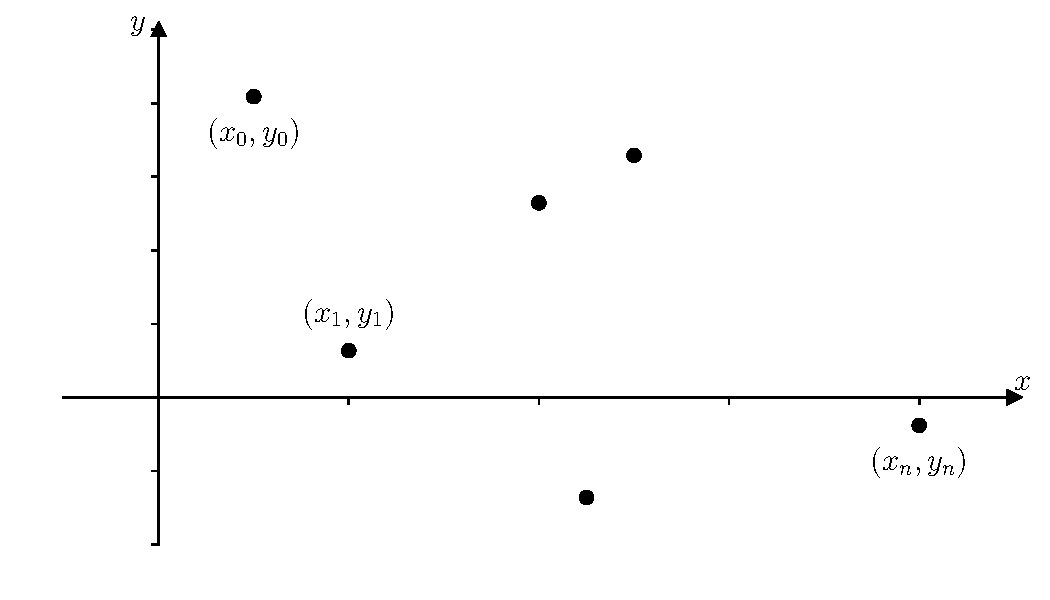
\includegraphics[width=0.7\textwidth]{figures/ch3_scatter.pdf} 
	  \caption{Scatter of $n+1$ points that we wish to fit.} \label{fig:ch3_scatter}
	\end{center}
\end{figure}
We may want to estimate what happens between the points. In this case it will be useful to have a function that agrees with the given data, but is defined for \textit{any} $x$ whatsoever. In this chapter we will consider polynomials to fill this role. Recall the definition of a polynomial of degree $n$
\begin{align*}
p(x) = a_0 + a_1 x + a_2 x^2 + \cdots + a_n x_n^n = \sum_{k=0}^n a_k x^k.
\end{align*}

As another motivation, we may be given a function $f(x)$ instead of data points. It can be computationally useful to estimate this function as a polynomial. Why? Maybe the function doesn't have a closed form. Maybe it takes a lot of computational power to give $f(x)$ at any particular $x$. In such a case you can compute a finite set of points $\{ (x_0,f(x_0))$, $(x_1,f(x_1))$, $\dots$, $(x_n,f(x_n)) \}$ that we can then use a polynomial to fit. The polynomial could then be used at a much reduced computational expense. On top of that, polynomials are analytically differentiable, which can be useful.


\section{Piece-wise linear fit}
We start with the simplest function that agrees with a set of data points: the \textit{piece-wise linear} fit that simply connects all the data points by straight lines, as sketched in figure~\ref{fig:ch3_piecewise}.
\begin{figure}[H]
	\begin{center}
	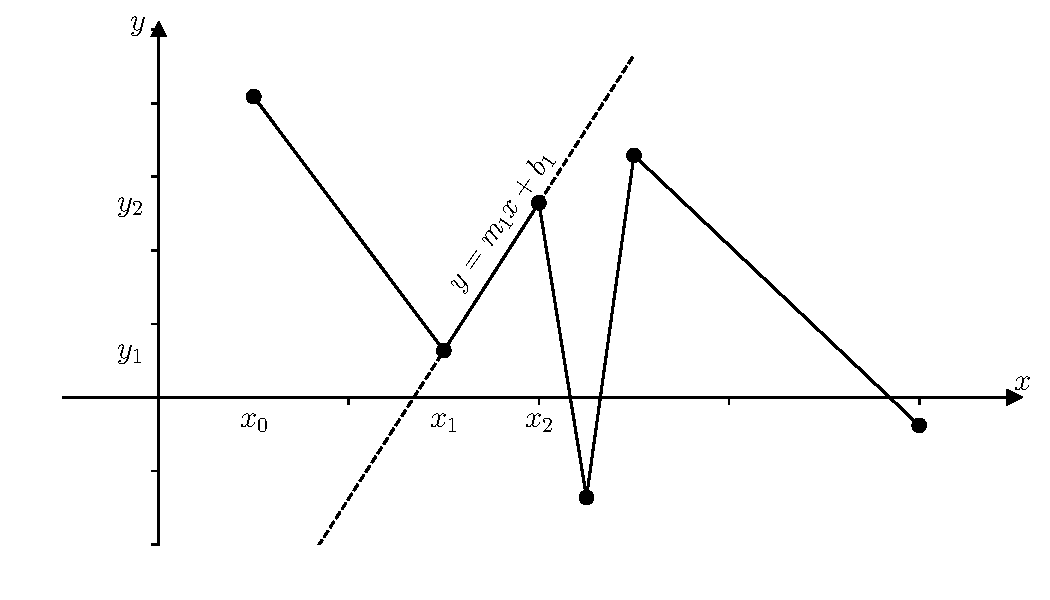
\includegraphics[width=0.8\textwidth]{figures/ch3_piecewise.pdf} 
	  \caption{Sketch of a piece-wise linear fit to some data points. The straight line connecting the 2nd and 3rd data points is highlighted.} \label{fig:ch3_piecewise}
	\end{center}
\end{figure}
It's necessary to order the data points in increasing $x$ coordinate, or else the resulting fit will be multi-valued, and thus not well defined. Then, for each pair of adjacent data points $(x_k,y_k)$ and $(x_{k+1},y_{k+1})$ we must define a straight line equation $y = m_k x + b_k$ for the interval between these points $x\in [x_k,x_{k+1}]$. The slope is given by ``rise over run'' for these two points
\begin{align*}
\boxed{ m_k = \frac{ y_{k+1}-y_{k} }{ x_{k+1}-x_{k} } }
\end{align*}
and then we get the $y$-intercept by using the straight line equation at either of the two data points
\begin{align*}
y(x_k) = y_k = m_k x_k + b_k \\
\implies \boxed{ b_k = y_k - m_k x_k} \\
(\text{or } b_k = y_{k+1} - m_k x_{k+1}).
\end{align*}
As defined above we have a function \textit{between} the data points. In principle we can just extend the first straight line infinitely to the left, $(-\infty,x_0]$, and also the last straight line infinitely to the right, $[x_n,\infty)$, in order to have a function defined for all $x\in \mathbb{R}$. Usually this is not a good idea.

\exemple{\upline}
{
	Find the piece-wise linear fit to the data: $\{ (1,1)$, $(2,3)$, $(3,2)$, $(4,3) \}$.
	
	For data points $(1,1)$, $(2,3)$:
	\begin{align*}
	& m_1 = \frac{3-1}{2-1} = 2 \\
	& b_1 = 1 - 2\times 1 = -1 \\
	& \implies y = 2x - 1
	\end{align*}
	
	For data points $(2,3)$, $(3,2)$:
	\begin{align*}
	& m_1 = \frac{2-3}{3-2} = -1 \\
	& b_1 = 3 - -1 \times 2 = 5 \\
	& \implies y = -x + 5
	\end{align*}
	
	For data points $(3,2)$, $(4,3)$:
	\begin{align*}
	& m_1 = \frac{3-2}{4-3} = 1 \\
	& b_1 = 2 - 1\times 3 = -1 \\
	& \implies y = x - 1
	\end{align*}
	
	So we can define the function on any $x$ between the first and last data point
	\begin{align*}
	y(x) = 
	\begin{cases}
	2x - 1 & \text{for } x\in [1,2] \\
	-x + 5 & \text{for } x\in [2,3] \\
	 x - 1 & \text{for } x\in [3,4] 
	\end{cases}
	\end{align*}
}{\downline}


\section{Lagrangian interpolation}
In this method, we fit a smooth polynomial through the scattering of points. Recall the figure~\ref{fig:ch3_scatter}, where we have $n+1$ pairs of numbers $(x_k,y_k)$. Let's start with a theorem

\theorem{LAGRANGE INTERPOLATION }{}
{Given the $n+1$ unique points $(x_0,y_0)$, $(x_1,y_1)$, $\dots$, $(x_n,y_n)$, there is a unique polynomial of degree at most $n$ passing through each point. That is, 
\begin{gather*}
\exists p_n(x) \in \mathcal{P}_n \\
\text{such that}\\ 
p_n(x_k)=y_k \quad \forall k.
\end{gather*}
}

We'll spend the rest of this section constructing this unique polynomial, called the \textit{Lagrange polynomial}.

First let's consider a couple of trivial cases. If we have just 1 point, $(x_0,y_0)$, then the degree 0 polynomial
\begin{align*}
p_0(x) = y_0
\end{align*}
will pass through the point. Though there are infinite straight lines that could go through this single point, this horizontal line is the only \textit{degree 0 polynomial}. When we have 2 points $(x_0,y_0)$ and $(x_1,y_1)$ then the degree 1 polynomial Lagrange polynomial is just the straight line joining the two
\begin{align*}
& p_1(x) = mx + b \\
& \text{with} \quad m = \frac{y_1 - y_0}{x_1 - x_0} \quad \text{and} \quad  b = m x_0 - y_0.
\end{align*}
These two trivial cases are shown in figure~\ref{fig:ch3_lagrange_n0_n1}.
\begin{figure}[H]
	\begin{center}
	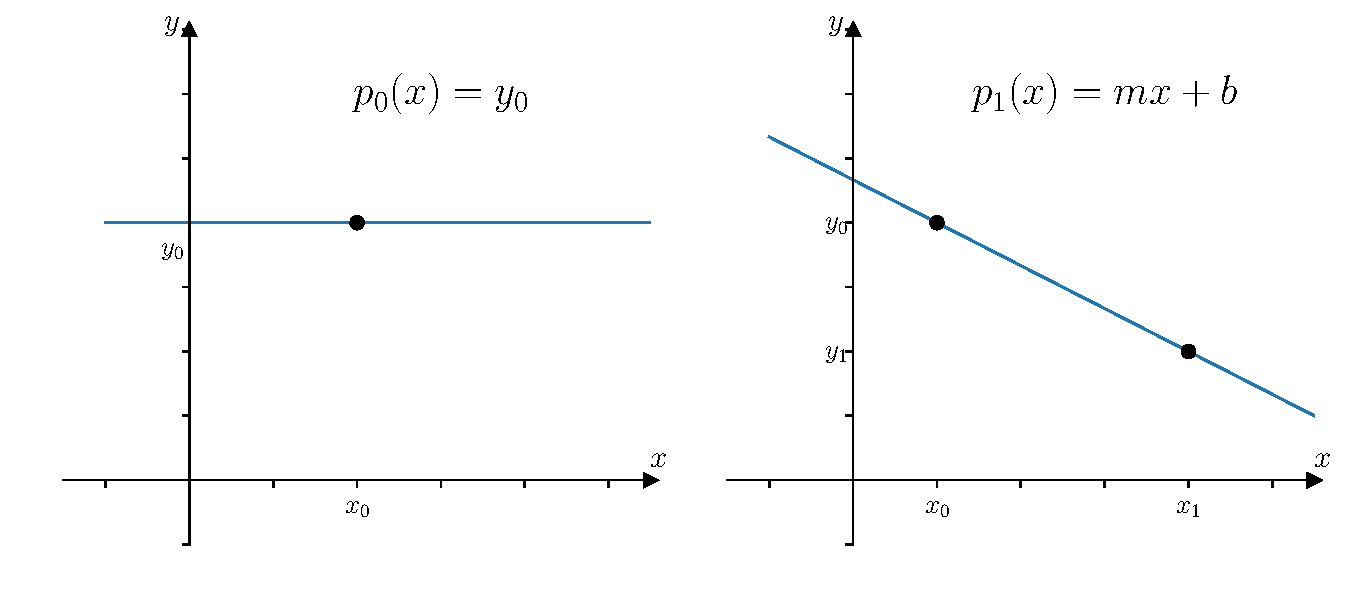
\includegraphics[width=\textwidth]{figures/ch3_lagrange_n0_n1.pdf} 
	  \caption{Trivial Lagrange polynomials for $n=0$ and $n=1$.} \label{fig:ch3_lagrange_n0_n1}
	\end{center}
\end{figure}

Ok, let's construct this unique polynomial for when we have more than 2 points. First, we choose one of the points, so $(x_k, y_k)$, and construct a polynomial, call it $L_k(x)$, that passes through 1 at this $x$, and goes through zero at all the other positions $x_i$ for $i\neq k$. That is, $L_k(x)$ must pass through the points $(x_k,1)$ and $(x_i,0)$ for all $i\neq k$. This polynomial is sketched in figure~\ref{fig:ch3_lagrange_Lk}.
\begin{figure}[H]
	\begin{center}
	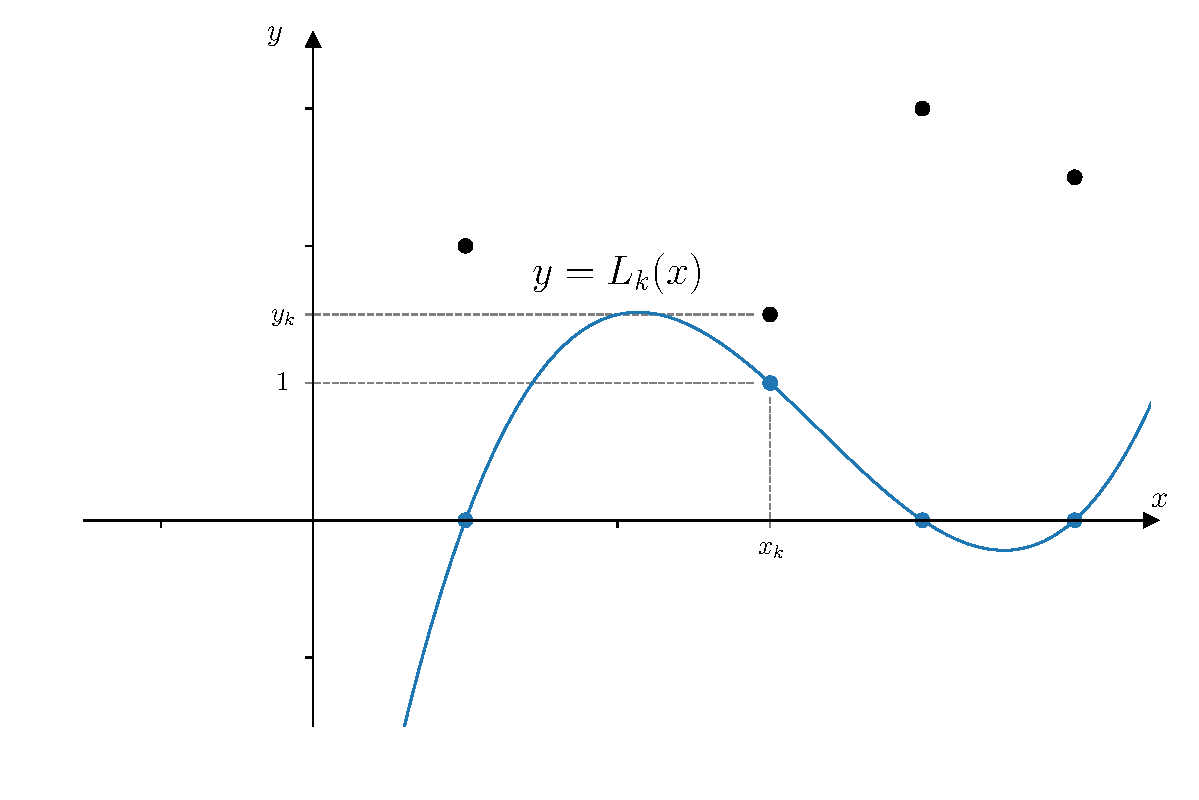
\includegraphics[width=0.6\textwidth]{figures/ch3_lagrange_Lk.pdf} 
	  \caption{.} \label{fig:ch3_lagrange_Lk}
	\end{center}
\end{figure}

It's very simple to construct a polynomial that has zeros at chosen $x$ values:
\begin{align*}
L_k(x) \propto (x-x_0)(x-x_1)\times \dots \times(x-x_{k-1})(x-x_{k+1})\times \dots \times(x-x_{n}).
\end{align*}
Notice we have excluded a term like $(x-x_k)$ to ensure that $L_k(x)$ \textit{does not} equal 0 at $x=x_k$. Including the proportionality constant, we then have
\begin{align*}
L_k(x) = C_k \prod_{i\neq k} (x-x_i).
\end{align*}
If you're not familiar with the ``big pie'' notation, it is the multiplicative version of the ``big sigma'' summation symbol $\Sigma$. Formally it is
\begin{align*}
\prod_{i=j}^{N} a_i = a_j \times a_{j+1} \times a_{j+2} \times \cdots \times a_{N-1} \times a_{N}.
\end{align*}
It just means that we multiply the following expression by itself over the indices provided. Look at the previous expression for $L_k(x)$ to see what the $\prod$ symbol is replacing.

Now, we can determine the constant $C_k$ by following our other desired property of $L_k(x)$, that it passes through $(x_k,1)$. This means
\begin{align*}
& L_k(x_k) = 1 \\
& \implies C_k \prod_{i\neq k} (x_k-x_i) = 1 \\
& \implies C_k  = \frac{1}{\prod_{i\neq k} (x_k-x_i)}
\end{align*}
So now we can write the definition of $L_k(x)$ in terms of the coordinates we are trying to fit
\begin{align*}
L_k(x) = \frac{\prod_{i\neq k} (x-x_i)}{\prod_{i\neq k} (x_k-x_i)}  = \prod_{i\neq k} \frac{x-x_i}{x_k-x_i} 
\end{align*}
Look at this function carefully. The denominator will be a multiplication of differences of known numbers, and so it will result in some number. The numerator is a function of $x$. We'll see in examples how this works in practice, but it really is just a number multipled by a polynomial, cleverly constructed to pass through certain points.

Now, this function passes through $(x_k,1)$ and $(x_i,0)$ for all $i\neq k$. If we multiply $L_k(x)$ by $y_k$, we will have a new polynomial that passes through $(x_k,y_k)$ and doesn't change the other points that still must pass through zero. This, therefore, nicely gives us the properties we wanted from the beginning 
\begin{align*}
y_k L_k(x) = 
\begin{cases}
y_k & \quad \text{if } x=x_k \\
0 & \quad \text{if } x=x_i \text{ for } i\neq k. 
\end{cases}
\end{align*} 
Now we only have to add up a series of these polynomials, giving us a new polynomial, that passes through every point we want. This is the \textit{Lagrange polynomial}:
\begin{align*}
\boxed{p(x) = \sum_{k=0}^n y_k L_k(x)}
\end{align*}
The components of the polynomial, $L_k(x)$, are called \textit{Lagrange basis polynomials}. A sketch of a Lagrange polynomial and its basis polynomials is shown in figure~\ref{fig:ch3_lagrange_total}.
\begin{figure}[H]
	\begin{center}
	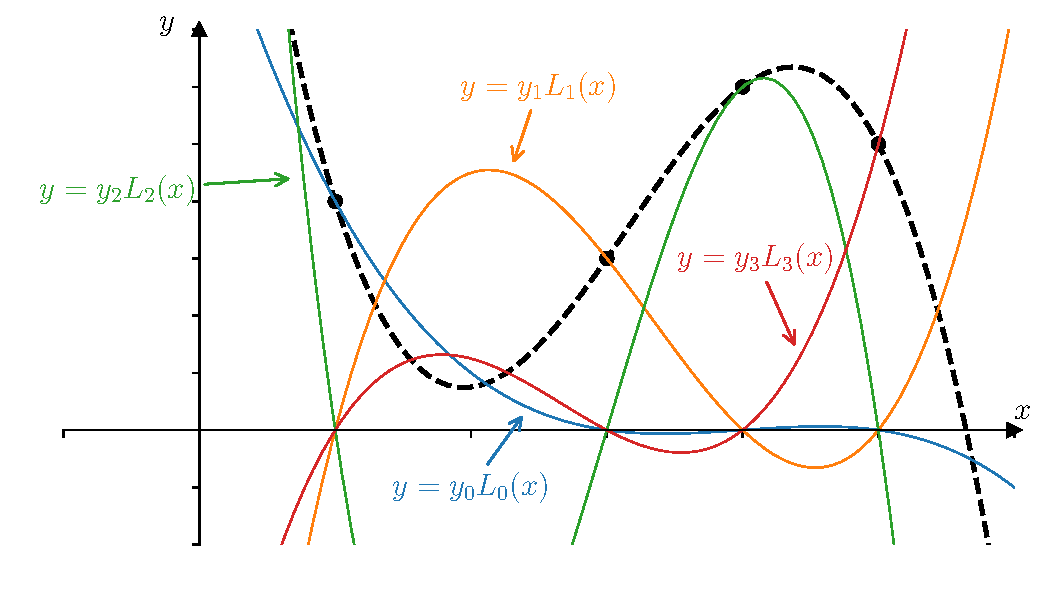
\includegraphics[width=0.8\textwidth]{figures/ch3_lagrange_total.pdf} 
	  \caption{Terms of the Lagrange polynomial. Note that each coloured line passes through exactly 1 of the desired interpolation points, while passing through zero at the location of all the others. The dashed line is the addition of the other 4 lines, and thus passes through each interpolation point.} \label{fig:ch3_lagrange_total}
	\end{center}
\end{figure}

\exemple{\upline}
{
	Let's find the Lagrange polynomial that passes through the points in 
	\begin{align*}
	\{(x_0,y_0),(x_1,y_1),(x_2,y_2),(x_3,y_3)\}=\{(1,1),(2,3),(3,2),(4,3)\}.
	\end{align*}
	Since there are 4 points to fit, we form 4 basis polynomials
	\begin{align*}
	L_0(x) &= \frac{(x-2)(x-3)(x-4)}{(1-2)(1-3)(1-4)}  = -\frac{1}{6}(x-2)(x-3)(x-4) \\ \\
	L_1(x) &= \frac{(x-1)(x-3)(x-4)}{(2-1)(2-3)(2-4)}  =  \frac{1}{2}(x-1)(x-3)(x-4) \\ \\
	L_2(x) &= \frac{(x-1)(x-2)(x-4)}{(3-1)(3-2)(3-4)}  = -\frac{1}{2}(x-1)(x-2)(x-4) \\ \\
	L_3(x) &= \frac{(x-1)(x-2)(x-3)}{(4-1)(4-2)(4-3)}  =  \frac{1}{6}(x-1)(x-2)(x-3)
	\end{align*} 
	Stare at each polynomial until you recognise the patterns. In this first step, the denominator is a copy/paste of the numerator, but $x$ is replaced with $x_k$ where $k$ is the index of the basis polynomial you are considering. Finally, we must add up these basis polynomials multipled by the $y$ values of the fitting points
	\begin{align*}
	p(x) &= 1\times L_0(x) + 3\times L_1(x) + 2\times L_2(x) + 4\times L_3(x)  \\
	 &= -\frac{1}{6}(x-2)(x-3)(x-4) + \frac{3}{2}(x-1)(x-3)(x-4) \\
		& - (x-1)(x-2)(x-4) + \frac{2}{3}(x-1)(x-2)(x-3)
	\end{align*}
}{\downline}




\subsection{Interpolation error estimation}
We can use a Lagrange polynomial to approximate a function $f(x)$ by sampling it at $n+1$ points $x_0$, \dots, $x_n$. That is, we take as data points $(x_0,f(x_0))$, $(x_1,f(x_1))$, \dots, $(x_n,f(x_n))$. If the function is continuous on the interval of the interpolation $[x_0,x_n]$, and its derivative of order $n+1$ exists and is also continuous on that interval, then the interpolation error is bounded:
\begin{align*}
|f(x) - p_n(x)| \leq \frac{M_{n+1}}{(n+1)!} \left| \prod_{i=0}^n (x-x_i) \right|
\end{align*}
where 
\begin{align*}
M_{n+1} = \max_{\alpha \in [x_0,x_n]} \left| f^{(n+1)}(\alpha)\right|
\end{align*}

%%%%%%%%%%%%%%%%%%%%%%%%%%%%%%%%%%%%%%%%%%%%%%
%%%%%%%%%%%%%%%%%%%%%%%%%%%%%%%%%%%%%%%%%%%%%%
%%%%%%%%%%%%%%%%%%%%%%%%%%%%%%%%%%%%%%%%%%%%%%
%%%%%%%%%%%%%%%%%%%%%%%%%%%%%%%%%%%%%%%%%%%%%%






%%%%%%%%%%%%%%%%%%%%%%%%%%%%%%%%%%%%%%%%%%%%%%
%%%%%%%%%%%%%%%%%%%%%%%%%%%%%%%%%%%%%%%%%%%%%%
%%%%%%%%%% NEWTONIAN INTERPOLATION %%%%%%%%%%%
%%%%%%%%%%%%%%%%%%%%%%%%%%%%%%%%%%%%%%%%%%%%%%
%%%%%%%%%%%%%%%%%%%%%%%%%%%%%%%%%%%%%%%%%%%%%%
\section{Newtonian interpolation}
There is a weakness to the Lagrangian method for finding the interpolation polynomial. Consider a set of $n+1$ data points $(x_0,y_0), (x_1,y_1), \dots, (x_n,y_n)$, so that the Lagrange polynomial is
\begin{align*}
p_n(x) = \sum_{k=0}^n y_k \prod_{i\neq k} \frac{x-x_i}{x_k-x_i} 
\end{align*}
what happens if we add data point $(x_{n+1},y_{n+1})$, as pictured below?
\begin{figure}[H]
	\begin{center}
	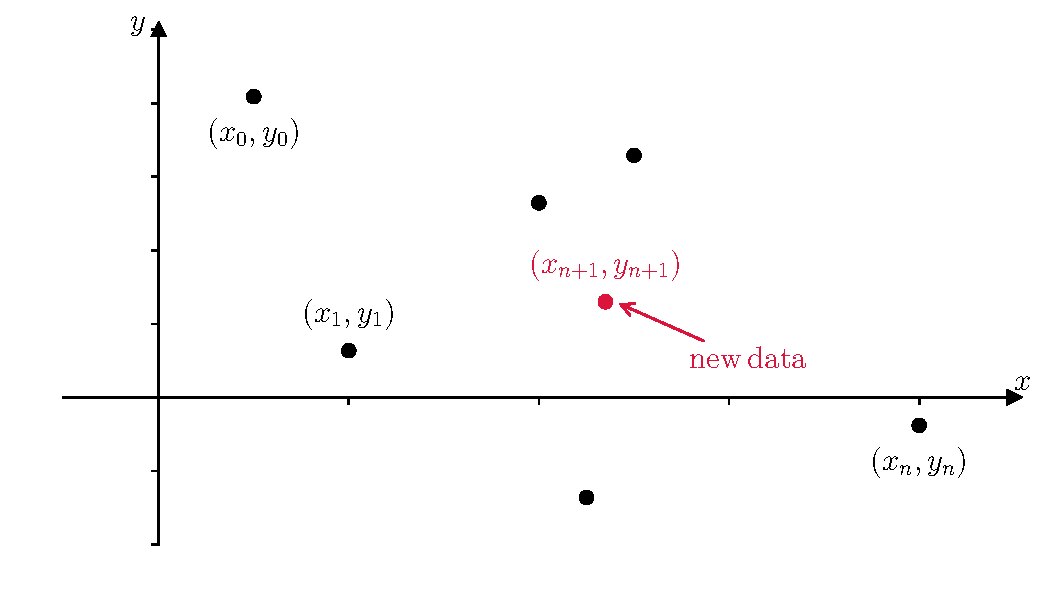
\includegraphics[width=0.8\textwidth]{figures/ch3_newton_purpose.pdf} 
	  \caption{} \label{fig:ch3_newton_purpose}
	\end{center}
\end{figure}

Well we would have to recompute all the Lagrange basis polynomials again to find $p_{n+1}$. This is obviously cumbersome, so we would like a method for \textit{sequentially} building the unique interpolation polynomial out of the previous polynomial with 1 less point and therefore 1 lower degree. That is, we want a scheme
\begin{align}\label{eq:ch3_newton_scheme}
p_{n+1}(x) = p_n(x) + q_{n+1}(x), \quad q_{n+1}(x) \in \mathcal{P}_{n+1}.
\end{align}
Now, the new polynomial must pass through all of the old points, so
\begin{align*}
p_{n+1}(x_k) = y_k \quad {\rm for} \, k=0,1,\dots,n.
\end{align*}
We also have that the old polynomial obviously passes through the old points
\begin{align*}
p_n(x_k) = y_k \quad {\rm for} \, k=0,1,\dots,n.
\end{align*}
Hence equation~\ref{eq:ch3_newton_scheme} evaluated at one of the data points gives
\begin{align*}
 p_{n+1}(x_k) &= p_n(x_k) + q_{n+1}(x_k) \\
 y_k &= y_k + q_{n+1}(x_k).
\end{align*}
So we have the constraint
\begin{align*}
q_{n+1}(x_k) = 0 \quad {\rm for} \, k=0,1,\dots,n.
\end{align*}
This means the general form of this extension polynomial is
\begin{align*}
q_{n+1}(x) = C_{n+1} \prod_{i=0}^{n} (x-x_i)
\end{align*}
for some constant $C_{n+1}$. Now the new polynomial, $p_{n+1}$ must also pass through the new datapoint $(x_{n+1},y_{n+1})$, giving
\begin{align*}
p_{n+1}(x_{n+1}) = y_{n+1}
\end{align*}
and hence
\begin{align*}
& y_{n+1} = p_n(x_{n+1}) + q_{n+1}(x_{n+1}) \\
&\implies C_{n+1} \prod_{i=0}^{n} (x_{n+1}-x_i) = y_{n+1} - p_n(x_{n+1}).
\end{align*}
This gives us an expression for this constant in terms of known values
\begin{align*}
\boxed{C_{n+1} = \frac{y_{n+1} - p_n(x_{n+1})}{\prod_{i=0}^{n} (x_{n+1}-x_i)}. }
\end{align*}
And so the Newtonian interpolation polynomial is given recursively as:
\begin{align}\label{eq:ch3_newton_scheme_explicit}
\boxed{p_{n+1}(x) = p_n(x) + C_{n+1}\prod_{i=0}^{n} (x-x_i).}
\end{align}
Let's look at this expression sequentially. The zeroth term is simple, it's forced to be a 0 degree polynomial passing through the point $(x_0,y_0)$. That is, it must be $p_0(x)=y_0$. This starts us off and let's us use equation~\ref{eq:ch3_newton_scheme_explicit}
\begin{align*}
p_1(x) &= y_0 + C_1(x-x_0) \\
%
p_2(x) &= y_0 + C_1(x-x_0) + C_2(x-x_0)(x-x_1) \\
%
&\vdots \\
%
p_{n+1}(x) &= y_0 + C_1(x-x_0) + C_2(x-x_0)(x-x_1) + \cdots +  C_{n+1}(x-x_0)(x-x_1)\times \dots \times (x-x_n)
\end{align*}

Now, $C_{n+1}$ as given above is horribly impractible. Let's demonstrate that by finding $C_1$ and $C_2$ in the general case before looking at a much better method!
\begin{align*}
C_1 &= \frac{y_1 - p_0(x_1)}{x_1-x_0} = \frac{y_1 - y_0}{x_1-x_0} \\
C_2 &= \frac{y_2 - p_1(x_2)}{(x_2-x_0)(x_2-x_1)} \\
%
&= \frac{y_2 - (y_0 + C_1(x_2-x_0))}{(x_2-x_0)(x_2-x_1)} \\
%
&= \frac{y_2 - y_0 - \frac{y_1 - y_0}{x_1-x_0}(x_2-x_0)}{(x_2-x_0)(x_2-x_1)} \\
%
&= \frac{y_2 - y_0}{(x_2-x_0)(x_2-x_1)} - \frac{y_1 - y_0}{(x_1-x_0)(x_2-x_1)}
%
\end{align*}
You see that the complexity builds up quickly. Try to write down $C_3$. But, there is a nice trick to quickly compute these coefficients, called \textit{divided differences}.

First, notationally we will replace the $C_{n+1}$ with
\begin{align*}
C_{n+1} = [y_0,\dots,y_n,y_{n+1}].
\end{align*}
This turns out to have a nice pattern involving recursive differences
\begin{align*}
C_0 &= [y_0] = y_0 \\
%
C_1 &= [y_0,y_1] = \frac{y_1 - y_0}{x_1-x_0} \\
%
C_2 &= [y_0,y_1,y_2] = \frac{[y_1,y_2] - [y_0,y_1]}{x_2-x_0} \\
%
C_3 &= [y_0,y_1,y_2,y_3] = \frac{[y_1,y_2,y_3] - [y_0,y_1,y_2]}{x_3-x_0} \\
%
&\vdots \\
%
C_{n+1} &= [y_0,\dots,y_n,y_{n+1}] = \frac{[y_1,\dots,y_{n+1}] - [y_0,\dots,y_{n}]}{x_{n+1}-x_0}.
\end{align*}
Before we make this clearer, let's check that it gives the right expression for $C_2$, that we found earlier.
\begin{align*}
C_2 &= \frac{[y_1,y_2] - [y_0,y_1]}{x_2-x_0} \\
%
&= \frac{\frac{y_2 - y_1}{x_2-x_1}  - \frac{y_1 - y_0}{x_1-x_0} }{x_2-x_0}  \\
%
&= \frac{y_2 - y_1}{(x_2-x_1)(x_2-x_0)} - \frac{y_1 - y_0 }{(x_1-x_0)(x_2-x_0)} \\
%
&= \frac{y_2 - y_0 + y_0 - y_1}{(x_2-x_1)(x_2-x_0)} - \frac{y_1 - y_0 }{(x_1-x_0)(x_2-x_0)}    \\
%
&= \frac{y_2 - y_0}{(x_2-x_1)(x_2-x_0)}- \frac{y_1 - y_0}{(x_2-x_1)(x_2-x_0)} - \frac{y_1 - y_0 }{(x_1-x_0)(x_2-x_0)} \\
%
&= \frac{y_2 - y_0}{(x_2-x_1)(x_2-x_0)}- \frac{y_1 - y_0}{x_2-x_0}\left(\frac{1}{x_2-x_1} +\frac{1}{x_1-x_0} \right) \\
%
&= \frac{y_2 - y_0}{(x_2-x_1)(x_2-x_0)}- \frac{y_1 - y_0}{(x_2-x_1)(x_1-x_0)}.
\end{align*}
It took some tricks but we got there, it's the same expression!

So, all we have done so far is replace one weird expression, the $C_{n+1}$, with another, $[y_0,\dots,y_n]$. If we compute these new things the interpolation polynomial is given by
\begin{align*}
p_{n+1}(x) &= [y_0] + [y_0,y_1](x-x_0) + [y_0,y_1,y_2](x-x_0)(x-x_1) + \cdots \\
& \quad + [y_0,\dots,y_{n+1}](x-x_0)(x-x_1)\times \cdots \times (x-x_n).
\end{align*}

Now we come to the heart of the method. These coefficients can be organised into a table that makes their computation actually clear:

\noindent \fbox{\begin{minipage}{\linewidth}
\underline{\textbf{Table of divided differences for Newtonian interpolation}}
\begin{figure}[H]
\begin{tabular}{ll|lll}
$x_0$ & $[y_0]$ &             &                 & \\ 
      &         & $[y_0,y_1]$ &                 & \\ 
$x_1$ & $[y_1]$ &             & $[y_0,y_1,y_2]$ & \\ 
      &         & $[y_1,y_2]$ &                 & $[y_0,y_1,y_2,y_3]$ \\ 
$x_2$ & $[y_2]$ &             & $[y_1,y_2,y_3]$ & \\ 
      &         & $[y_2,y_3]$ &                 & \\ 
$x_3$ & $[y_3]$ &             &                 & \\
\vdots & \vdots & \vdots & \vdots & \vdots
\end{tabular}
\end{figure}

\end{minipage}}

And of course it will become clearer what this table means with multiple usages.

\exemple{\upline}{
Given the data $\{(1,2), (2,2), (3,1), (4,3) \}$, determine the interpolation polynomial using the table of divided differences.

The table of divided differences is
\begin{figure}[H]
\begin{tabular}{ll|lll}
$x_k$ & $y_k$ &  &  & \\ \hline
$1$ & \fbox{2} &                      &                                 & \\ 
    &   & $\frac{2-2}{2-1}=\fbox{0}$  &                                 & \\ 
$2$ & 2 &                      & $\frac{-1-0}{3-1}=\fbox{-1/2}$ & \\ 
    &   & $\frac{1-2}{3-2}=-1$ &                                 &  $\frac{\frac{3}{2}--\frac{1}{2}}{4-1}=\fbox{2/3}$ \\ 
$3$ & 1 &                      & $\frac{2--1}{4-2}=\frac{3}{2}$  & \\ 
    &   & $\frac{3-1}{4-3}=2$  &                                 & \\ 
$4$ & 3 &                      &                                 &
\end{tabular}
\end{figure}
In the boxes are the coefficients we need for the interpolation polynomial
\begin{align*}
p(x) &= 2 + 0(x-1) - \frac{1}{2}(x-1)(x-2) + \frac{2}{3}(x-1)(x-2)(x-3) \\
&= 2 - \frac{1}{2}x^2 + \frac{3}{2}x - 1 +\frac{2}{3}x^3 - 4 x^2 + \frac{22}{3}x - 4 \\
&= -3 + \frac{53}{6}x - \frac{9}{2}x^2 + \frac{2}{3}x^3
\end{align*}
}{\downline}

Now let's do an example to see that \textit{the order of the data doesn't matter}.

\exemple{\upline}{
Given the data $\{(1,2), (3,1), (4,3) \}$, construct the table of divided differences. Then add the datapoint $(2,2)$ to find the interpolation polynomial.

The table of divided differences for the 3 points is
\begin{figure}[H]
\begin{tabular}{ll|lll}
$x_k$ & $y_k$ &  &  & \\ \hline
$1$ & $\fbox{2}$ &                               & & \\ 
    &            & $\frac{1-2}{3-1}=\fbox{-1/2}$ & & \\ 
$3$ & $1$        &                               & $\frac{2--\frac{1}{2}}{4-1}=\fbox{5/6}$  & \\ 
    &            & $\frac{3-1}{4-3}=2$           & &  \\ 
$4$ & $3$        &                               & & \\ 
\end{tabular}
\end{figure}
In the boxes are the coefficients we need for the degree 2 polynomial fitting just these 3 points
\begin{align*}
p_2(x) &= 2 - \frac{1}{2}(x-1) + \frac{5}{6}(x-1)(x-3) \\
&= 2 - \frac{1}{2}x + \frac{1}{2} +\frac{5}{6}x^2 -\frac{10}{3}x + \frac{5}{2}\\
&= 5 - \frac{23}{6}x + \frac{5}{6}x^2
\end{align*}
Now we add the new point $(2,2)$ by simply attaching it to the previous table
\begin{figure}[H]
\begin{tabular}{ll|lll}
$x_k$ & $y_k$ &  &  & \\ \hline
$1$ & $2$ &                               & & \\ 
    &     & $\frac{1-2}{3-1}=-\frac{1}{2}$ & & \\ 
$3$ & $1$ &                               & $\frac{2--\frac{1}{2}}{4-1}=\frac{5}{6}$ & \\ 
    &     & $\frac{3-1}{4-3}=2$           &                                          & $\frac{\frac{3}{2}-\frac{5}{6}}{2-1}=\fbox{2/3}$ \\ 
$4$ & $3$ &                               & $\frac{\frac{1}{2}-2}{2-3}=\frac{3}{2}$  & \\ 
    &     & $\frac{2-3}{2-4}=\frac{1}{2}$ & &  \\ 
$2$ & $2$ &                               & & \\ 
\end{tabular}
\end{figure}
In the box is the coefficient we need to extend the degree 2 interpolation polynomial into the degree 3 polynomial that fits all 4 points
\begin{align*}
p_3(x) &= p_2(x) + \frac{2}{3}(x-1)(x-3)(x-4) \\
&= 5 - \frac{23}{6}x + \frac{5}{6}x^2 + \frac{2}{3}x^3 - \frac{16}{3}x^2 + \frac{38}{3}x - 8\\
&= -3 + \frac{53}{6}x - \frac{9}{2}x^2 + \frac{2}{3}x^3
\end{align*}
which is the same polynomial we found in the previous example! The order doesn't matter, and we can extend the polynomials one term at a time.
}{\downline}




%%%%%%%%%%%%%%%%%%%%%%%%%%%%
%%%%%%%%%%%%%%%%%%%%%%%%%%%%
%%%%%%%%%%%%%%%%%%%%%%%%%%%%
%%%% Exercises %%%%
%%%%%%%%%%%%%%%%%%%%%%%%%%%%
%%%%%%%%%%%%%%%%%%%%%%%%%%%%
%%%%%%%%%%%%%%%%%%%%%%%%%%%%
\exercises{
\section{Exercises}

\exercice{Given data $\{(1,2), (2,5), (3,3), (4,2)\}$}
\begin{enumerate}[label=\alph*)]
	\item Make a piece-wise linear interpolation of the given data.
	
	\item Find the unique polynomial of order less than 4 passing through each data point using the Lagrangian interpolation method.
	
	\item Find the unique polynomial of order less than 4 passing through each data point using the Newtonian interpolation method.
\end{enumerate}


\exercice{Given data $\{(1,2), (1.5,1.5), (3,2.5), (6,3)\}$}
\begin{enumerate}[label=\alph*)]
	\item Make a piece-wise linear interpolation of the given data.
	
	\item Find the unique polynomial of order less than 4 passing through each data point using the Lagrangian interpolation method.
	
	\item Find the unique polynomial of order less than 4 passing through each data point using the Newtonian interpolation method.
\end{enumerate}


\exercice{Estimate $f(x) = \log(x+2)$}
\begin{enumerate}[label=\alph*)]
	\item Make a piece-wise linear interpolation of $f(x)$ at positions $x \in [0,2,4,6]$.
	
	\item Give the Lagrangian polynomial of order less than 4 passing through $f(x)$ at positions $x \in [0,2,4,6]$.
	
	\item Use Newtonian interpolation to give the polynomial of order less than 4 passing through $f(x)$ at positions $x \in [0,1,5,6]$.
	
	\item Find the area under $f(x)$ between 0 and 6 by using the polynomials found in parts b and c. Compare to the analytic solution by directly integrating $f(x)$.
	
	\item Using your table of divided differences from part c, add 1 data point at $x=3$ to increase the polynomial order by 1.
\end{enumerate}


\exercice{Estimate $f(x) = e^x$}
\begin{enumerate}[label=\alph*)]
	\item Make a piece-wise linear interpolation of $f(x)$ at positions $x \in [-1,1,3,5]$.
	
	\item Give the Lagrangian polynomial of order less than 4 passing through $f(x)$ at positions $x \in [-1,0,4,5]$.
	
	\item Use Newtonian interpolation to give the polynomial of order less than 4 passing through $f(x)$ at positions $x \in [-1,1,3,5]$.
	
	\item Find the area under $f(x)$ between 0 and 6 by using the polynomials found in parts b and c. Compare to the analytic solution by directly integrating $f(x)$.
	
	\item Using your table of divided differences from part c, add 1 data point at $x=2$ to increase the polynomial order by 1.
\end{enumerate}
} % complete 28/06/22
%\chapter{Least-squares Extrapolation} \label{ch:leastsquares}

Sometimes we don't want to fit data with a curve that is forced to pass through every point. We might instead assume there is a simple relation underneath the data and \textit{noise} scatters the data around this relation. For example, see figure~\ref{fig:ch4_purpose}.

\begin{figure}[H]
	\begin{center}
	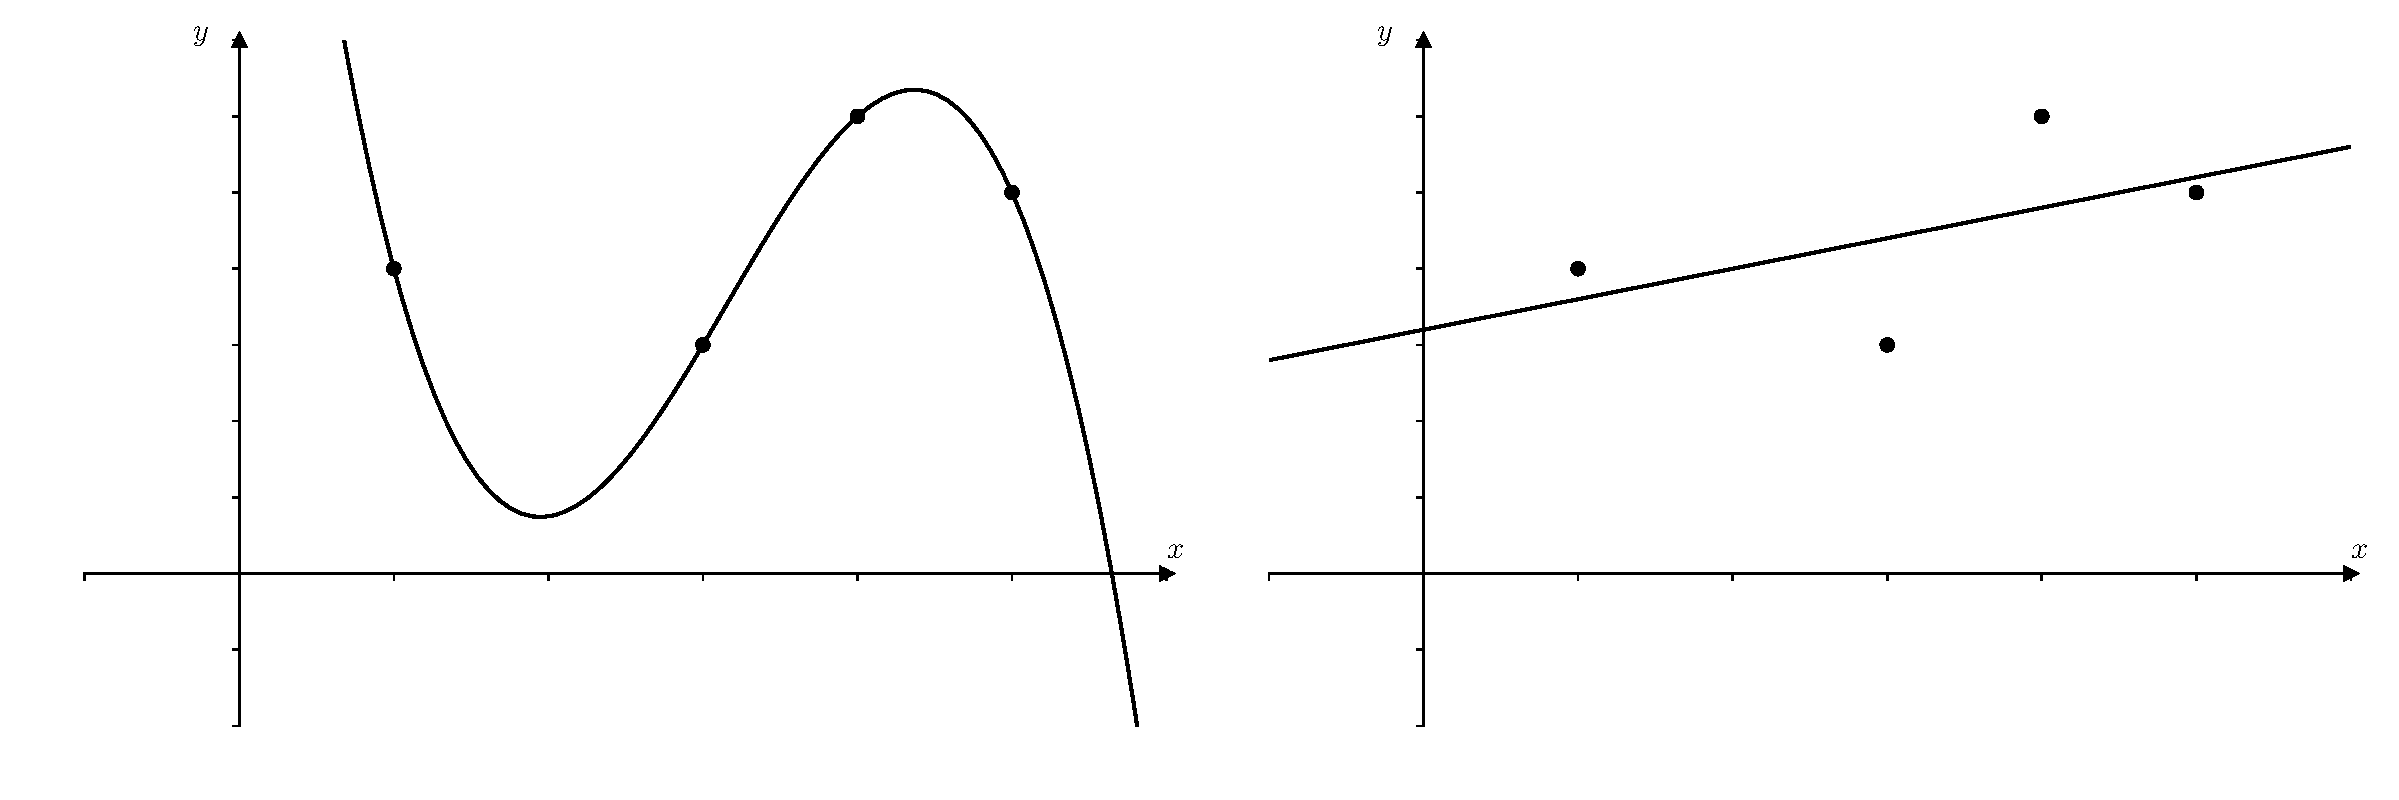
\includegraphics[width=\textwidth]{figures/ch4_least_squares_purpose.pdf} 
	  \caption{(Left) Lagrange polynomial passing through each point (right) simple line that roughly captures the trend of the data.} \label{fig:ch4_purpose}
	\end{center}
\end{figure}

If we see a rough trend in the data, we may want to predict what will happen outside of the data range. The Lagrange polynomial is bad at this, giving massive errors outside of the range of the given data. So, Lagrange is good for \textit{interpolation}, and in this chapter we will look at the method of least squares which is good for \textit{extrapolation}.

\section{Least-squares linear fitting}
Say you have $n+1$ data points $(x_k,y_k)$ for $k=0,1,2,\dots,n$. Imagine we want to \textit{fit} this data with a straight line. We want to find the best line $y=mx + b$, where best means to minimise the square of the \textit{residuals}:
\begin{align*}
r_k = y_k - y(x_k).
\end{align*}
Looking at figure~\ref{fig:ch4_defintion} you can see that the residual is the vertical distance between a data point and a straight line. So minimising the residuals is a way to choose a line that is closest to all the data points in some way. We minimise the square so that it doesn't matter whether the residual is positive or negative.

\begin{figure}[H]
	\begin{center}
	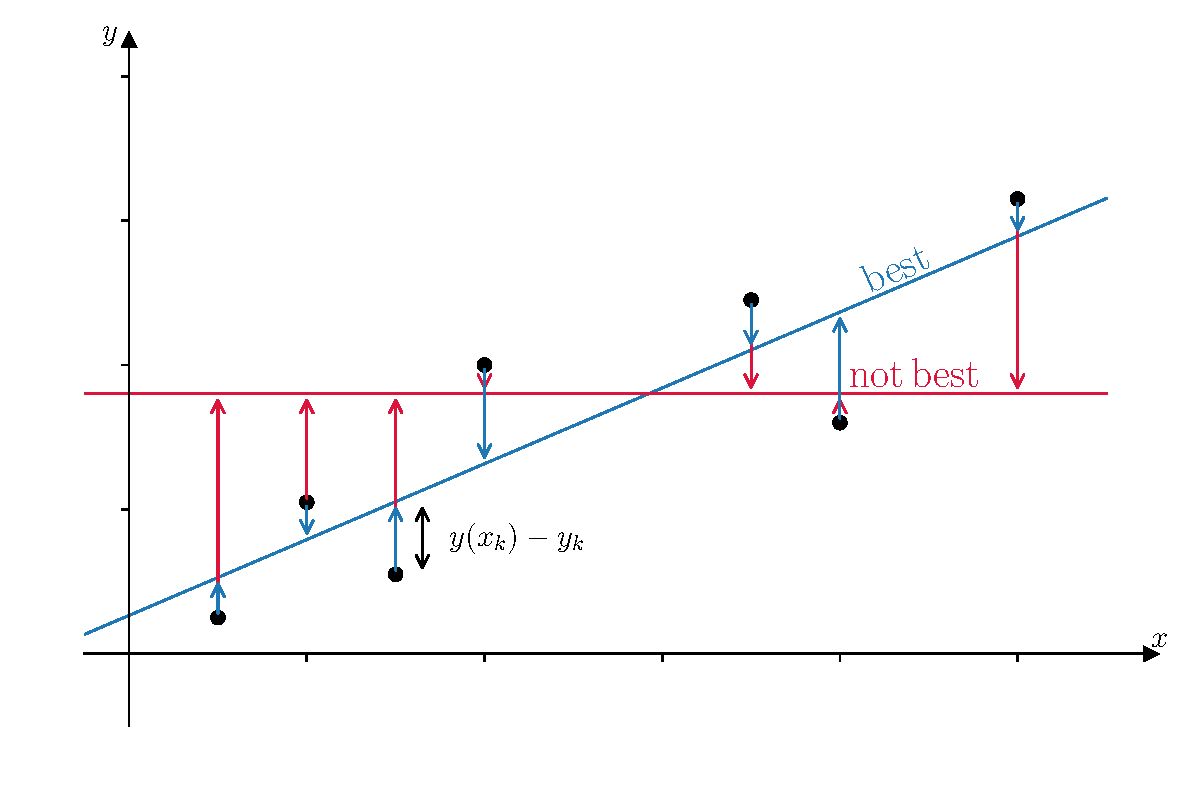
\includegraphics[width=0.7\textwidth]{figures/ch4_least_squares_defn.pdf} 
	  \caption{Two linear fits to the data points. The blue straight line minimises the collection of distances, $y(x_k)-y_k$, of each data point from the line. The red line is obviously worse.} \label{fig:ch4_defintion}
	\end{center}
\end{figure}

What are we changing when we say we are minimising the (square of the) residuals? We are adjusting a straight line, which means we are changing the slope ,$m$, and the vertical offset, $b$. So. let's define the sum of the square of the residuals as a two variable function in the variables $m$ and $b$
\begin{align*}
S(m,b) = \sum_{k=0}^n r_k^2 = \sum_{k=0}^n \left(y_k - y(x_k)\right)^2.
\end{align*}
This function is general for any fitting curve $y(x)$, but in this chapter we only use linear fits, so we can define the function $S$ as
\begin{align*}
S(m,b) = \sum_{k=0}^n \left(y_k - mx_k - b\right)^2.
\end{align*}

Recall that to find where a single-variable function, $f(x)$, is minimum (or maximum) you must find where its derivative is equal to zero. For multi-variate functions, we must find where its partial derivatives are zero. So we impose
\begin{align*}
\frac{\partial S}{\partial m} = 0 \\
\frac{\partial S}{\partial b} = 0.
\end{align*}
These partial derivatives are
\begin{align*}
\frac{\partial S}{\partial m} = \sum_{k=0}^n 2 r_k x_k = \sum_{k=0}^n 2 \left(y_k - mx_k - b\right) x_k\\
\frac{\partial S}{\partial b} = \sum_{k=0}^n 2 r_k = \sum_{k=0}^n 2 \left(y_k - mx_k - b\right)
\end{align*}
and so setting these to be zero, we must simultaneously solve
\begin{align}
\sum_{k=0}^n \left(y_k - mx_k - b\right) x_k = 0  \label{eq:dsdm}\\
\sum_{k=0}^n \left(y_k - mx_k - b\right) = 0 \label{eq:dsdb}
\end{align}


\exemple{\upline}
{
	Make a least-squares linear fit to the data: $\{ (1,1)$, $(2,3)$, $(3,2)$, $(5,3) \}$.
	
	\noindent We want $m$ and $b$ for $y(x) = mx + b$. The residuals are
	\begin{align*}
	r_0 &= 1 - m - b \\
	r_1 &= 3 - 2m - b \\
	r_2 &= 2 - 3m - b \\
	r_3 &= 3 - 5m - b
	\end{align*}
	
	The function to minimise is
	\begin{align*}
	S(m,b) &= r_0^2 + r_1^2 + r_2^2 + r_3^2\\
	&= 1 -   m -  b -   m +   m^2 +  mb -  b +  mb + b^2 + \\
	&  9 -  6m - 3b -  6m +  4m^2 + 2mb - 3b + 2mb + b^2 + \\
	&  4 -  6m - 2b -  6m +  9m^2 + 3mb - 2b + 3mb + b^2 + \\
	&  9 - 15m - 3b - 15m + 25m^2 + 5mb - 3b + 5mb + b^2.
	\end{align*}
	Finally, collecting all the terms we have
	\begin{align*}
	\boxed{S(m,b) = 23 - 56m -18b + 22mb + 39m^2 + 4b^2}
	\end{align*}
	The partial derivatives give
	\begin{align*}
	\frac{\partial S}{\partial m} &= -56 +22b + 78m = 0 \implies b=\frac{56-78m}{22} \\
	\frac{\partial S}{\partial b} &= -18 +22m + 8b = 0  \implies b=\frac{18-22m}{8}
	\end{align*}
	This eliminates $b$, allowing us to determine $m$
	\begin{align*}
	& \frac{56-78m}{22} = \frac{18-22m}{8} \\
	& 8(56 - 78m) = 22(18-22m)\\
	& 484m - 624m = 396 - 448 \\
	& m = \frac{52}{140} \sim 0.37
	\end{align*}
	and now plug this into either of the 2 equations for $b$
	\begin{align*}
	b \sim \frac{56-78\times 0.37}{22} \sim 1.23.
	\end{align*}
	So we have the least squares linear fit to the data
	\begin{align*}
	y = 0.37 x + 1.23.
	\end{align*}
}{\downline}

In this previous example we expanded the squares of residuals \textit{then} differentianted. It turns out to be easier to differentiate \textit{then} expand. Recall the partial derivative of $S$ with respect to $b$ gave us the condition
\begin{align*}
\sum_{k=0}^n \left(y_k - mx_k - b\right) = 0.
\end{align*}
This can be rearranged to
\begin{align*}
&\sum_{k=0}^n \left(y_k - mx_k\right) -  \sum_{k=0}^n b = 0 \\
&\sum_{k=0}^n \left(y_k - mx_k\right) -  (n+1) b = 0
\end{align*}
so that we have an expression for $b$
\begin{align*}
\boxed{b = \frac{1}{n+1}\sum_{k=0}^n \left(y_k - mx_k\right)}
\end{align*}

For the previous example with data $\{ (1,1)$, $(2,3)$, $(3,2)$, $(5,3) \}$, we have $n=3$, and this gives
\begin{align*}
b &= \frac{1}{4}\left( (1 - m) + (3-2m) + (2-3m) + (3-5m) \right) \\
&= \frac{9 - 11m}{4} = \frac{18 - 22m}{8}
\end{align*}
which is the same equation we had, but now we reached it faster.

The partial derivative with respect to $m$ gave us the condition
\begin{align*}
\sum_{k=0}^n x_k\left(y_k - mx_k - b\right) = 0.
\end{align*}
For this previous example this gives
\begin{align*}
& 1(1 - m - b) + 2(3-2m - b) + 3(2-3m - b) + 5(3-5m - b) = 0 \\
& 28 - 39m -11b = 0.
\end{align*}
This is the second equation that we got earlier, but now we reached it faster. Taking the derivatives before expanding is simpler because it removes the need to expand squared expressions.

But we can push this algebra further to create even simpler expressions for $b$ and $m$. So we start from the $b$ expression we just derived
\begin{align*}
b = \frac{1}{n+1}\sum_{k=0}^n y_k - m  \frac{1}{n+1}\sum_{k=0}^n x_k. 
\end{align*}
Now we note that the sum of a list of numbers, $x_k$, divided by how many numbers in that list is just the average value of the list, which we will denote $\bar{x}_k$. So we can write
\begin{align}
b = \bar{y}_k - m \bar{x}_k. \label{eq:offset1}
\end{align}
We insert this into equation~\ref{eq:dsdm} and clean things up
\begin{align*}
& \sum_{k=0}^n x_k\left(y_k - mx_k - b\right) = 0 \\
& \sum_{k=0}^n x_k\left(y_k - mx_k - \bar{y}_k + m \bar{x}_k\right) = 0 \\
& \sum_{k=0}^n \left( x_k \left(y_k - \bar{y}_k\right)   + m x_k\left(\bar{x}_k  - x_k\right) \right) = 0 \\
& \sum_{k=0}^n  x_k \left(y_k - \bar{y}_k\right)   + m \sum_{k=0}^n  x_k\left(\bar{x}_k  - x_k\right)  = 0.
\end{align*}
And this gives us an expression for $m$ that is independent of $b$
\begin{align*}
\boxed{  m   = \frac{\sum_{k=0}^n  x_k\left(\bar{y}_k - y_k\right)}{\sum_{k=0}^n  x_k \left(\bar{x}_k  - x_k \right) } }
\end{align*}
which can be plugged into equation~\ref{eq:offset1} to give an expression for $b$ that is independent of $m$
\begin{align*}
\boxed{b = \bar{y}_k - \bar{x}_k \frac{\sum_{k=0}^n  x_k\left(\bar{y}_k - y_k\right)}{\sum_{k=0}^n  x_k \left(\bar{x}_k  - x_k \right) } }
\end{align*}

These last two expressions are not necessarily easier to use in hand calculations, but they are very easy to code. A computer can take averages very easily, and so those two expressions might be more useful for creating a least-squares computer program.

\exemple{\upline}
{
	Make a least-squares linear fit to the data: $\{ (1,1)$, $(2,3)$, $(3,2)$, $(5,3) \}$. Same as the previous example, but with the new method.
	
	\noindent We need the averages of the $x_k$ and $y_k$:
	\begin{align*}
	\bar{x}_k &= \frac{1+2+3+5}{4} = \frac{11}{4} \\
	\bar{y}_k &= \frac{1+3+2+3}{4} = \frac{9}{4} 
	\end{align*}
	So we use the formula to calculate the slope
	\begin{align*}
	m   = \frac{1(\frac{9}{4}-1)+2(\frac{9}{4}-3)+3(\frac{9}{4}-2)+4(\frac{9}{4}-3)}{1(\frac{11}{4}-1)+2(\frac{11}{4}-2)+3(\frac{11}{4}-3)+5(\frac{11}{4}-5)} = \frac{-13/4}{-35/4} \sim 0.37
	\end{align*}
	Now we use this in the formula for the offset
	\begin{align*}
	b = \bar{y}_k - m \bar{x}_k \sim \frac{9}{4}  - 0.37 \times \frac{11}{4} \sim 1.23
	\end{align*}
	So we have the same least squares linear fit to the data
	\begin{align*}
	y = 0.37 x + 1.23.
	\end{align*}
	You decide whether this method is simpler or not.
}{\downline}


\section{Degree n polynomial least-squares}
We generalise the previous work by assuming a fitting polynomial of degree $p$:
\begin{align*}
y(x) = a_0 + a_1 x + a_2 x^2 + \dots + a_p x^p
\end{align*}
Then the sum of the square residuals function becomes a function of $p+1$ parameters
\begin{align*}
S(a_0, a_1, a_2, \dots, a_p) &= \sum_{k=0}^n \left( y(x_k) - y_k \right)^2 \\
&= \sum_{k=0}^n \left( a_0 + a_1 x_k + a_2 x_k^2 + \dots + a_p x_k^p - y_k \right)^2
\end{align*}
We now have $p+1$ partial derivatives to set to zero to find the minimised set of parameters:
\begin{align*}
\frac{\partial S}{\partial a_0} &= 2\sum_{k=0}^n \left( a_0 + a_1 x_k + a_2 x_k^2 + \dots + a_p x_k^p - y_k \right) \\
\frac{\partial S}{\partial a_1} &= 2\sum_{k=0}^n \left( a_0 + a_1 x_k + a_2 x_k^2 + \dots + a_p x_k^p - y_k \right) x_k \\
 & \,\vdots \\
\frac{\partial S}{\partial a_p} &= 2\sum_{k=0}^n \left( a_0 + a_1 x_k + a_2 x_k^2 + \dots + a_p x_k^p - y_k \right)  x_k^p
\end{align*}
Since all of these derivatives are set to zero, we can cancel the constant 2 in each equation, and we find a system of equations that is linear \textit{in the parameters}
\begin{align*}
 & \left(\sum_{k=0}^n 1\right) a_0 + \left(\sum_{k=0}^n x_k\right)a_1 +  \left(\sum_{k=0}^n  x_k^2\right)a_2 + \dots + \left(\sum_{k=0}^n  x_k^p \right)a_p  =  \sum_{k=0}^n y_k \\
 %
 & \left(\sum_{k=0}^n x_k\right) a_0 + \left(\sum_{k=0}^n x_k^2\right)a_1 +  \left(\sum_{k=0}^n  x_k^3\right)a_2 + \dots + \left(\sum_{k=0}^n  x_k^{p+1} \right)a_p  =  \sum_{k=0}^n y_k x_k \\
 %
 & \left(\sum_{k=0}^n x_k^2\right) a_0 + \left(\sum_{k=0}^n x_3\right)a_1 +  \left(\sum_{k=0}^n  x_k^2\right)a_4 + \dots + \left(\sum_{k=0}^n  x_k^{p+2} \right)a_p  =  \sum_{k=0}^n y_k x_k^2 \\
 %
 & \hspace{6cm} \vdots \\
 %
 & \left(\sum_{k=0}^n x_k^{p}\right) a_0 + \left(\sum_{k=0}^n x_k^{p+1}\right)a_1 +  \left(\sum_{k=0}^n  x_k^{p+2}\right)a_2 + \dots + \left(\sum_{k=0}^n  x_k^{2p} \right)a_p  =  \sum_{k=0}^n y_k  x_k^{p-1}
\end{align*}
This is better viewed as a matrix equation (and noting that $\dsum_{k=0}^n 1 = n+1$)
\begin{align*}
\begin{pmatrix}
n+1 & \dsum_{k=0}^n x_k & \dsum_{k=0}^n  x_k^2 & \cdots & \dsum_{k=0}^n  x_k^p   \\
%
\dsum_{k=0}^n x_k & \dsum_{k=0}^n x_k^2 & \dsum_{k=0}^n  x_k^3 & \cdots & \dsum_{k=0}^n  x_k^{p+1}   \\
%
\dsum_{k=0}^n x_k^2 & \dsum_{k=0}^n x_k^3 & \dsum_{k=0}^n  x_k^4 & \cdots & \dsum_{k=0}^n  x_k^{p+2}  \\
\vdots & \vdots & \vdots & \ddots & \vdots \\
%
\dsum_{k=0}^n x_k^p & \dsum_{k=0}^n x_k^{p+1} & \dsum_{k=0}^n  x_k^{p+2} & \cdots & \dsum_{k=0}^n  x_k^{2p}
\end{pmatrix}
%
\begin{pmatrix}
a_0 \\ a_1 \\ a_2 \\ \vdots \\ a_p
\end{pmatrix}
%
=
%
\begin{pmatrix}
\dsum_{k=0}^n y_k \\ \dsum_{k=0}^n y_k x_k \\ \dsum_{k=0}^n y_k x_k^2 \\ \vdots \\ \dsum_{k=0}^n y_k x_k^{p-1}
\end{pmatrix}
\end{align*}
Denoting this equation as $M \mathbf{a} = \mathbf{b}$, it can be shown (by a better mathematician) that $M$ is always an invertible matrix. So we can ``easily'' find the best-fit parameters with $\mathbf{a} = M^{-1} \mathbf{b}$.


\exemple{\upline}
{
	\noindent Make a 2nd degree polynomial least-squares fit to the data: $\{ (-1,2)$, $(2,-1)$, $(4,1)$, $(6,2) \}$. 
	
	\noindent In this problem $n=3$ ($n+1=4$ data points) and $p=2$ (degree 2 polynomial). We want a 2nd degree polynomial: $y(x) = a_0 + a_1 x + a_2 x^2$. The 2nd degree least-squares matrix equation, $M\mathbf{a} = \mathbf{b}$, is then
	\begin{align*}
	&
	\begin{pmatrix}
	4 & \dsum_{k=0}^3 x_k & \dsum_{k=0}^3  x_k^2 \\
	%
	\dsum_{k=0}^3 x_k & \dsum_{k=0}^3 x_k^2 & \dsum_{k=0}^3  x_k^3   \\
	%
	\dsum_{k=0}^3 x_k^2 & \dsum_{k=0}^3 x_k^3 & \dsum_{k=0}^3  x_k^4 
	\end{pmatrix}
	%
	\begin{pmatrix}
	a_0 \\ a_1 \\ a_2
	\end{pmatrix}
	%
	=
	%
	\begin{pmatrix}
	\dsum_{k=0}^n y_k \\ \dsum_{k=0}^n y_k x_k \\ \dsum_{k=0}^n y_k x_k^2 
	\end{pmatrix} \\
	%%
	%%
	%%
	\implies  M &=
	\begin{pmatrix}
	4 & -1+2+4+6 & 1+4+16+36 \\
	%
	-1+2+4+6 & 1+4+16+36 & -1+8+64+198   \\
	%
	1+4+16+36 & -1+8+64+198 & 1+16+256+1296
	\end{pmatrix} \\
	%
	&=
	\begin{pmatrix}
	4 & 11 & 57 \\
	%
	11 & 57 & 287   \\
	%
	57 & 287 & 1569
	\end{pmatrix} \\
	%%
	%%
	%%
	\text{and }  \mathbf{b} &=
	\begin{pmatrix}
	2-1+1+2 \\ 
	-2-2+4+12 \\ 
	2-4+16+72
	\end{pmatrix}
	%
	=
	\begin{pmatrix}
	4 \\ 
	12 \\ 
	86
	\end{pmatrix}
	\end{align*}
	The inverse of $M$ is
	\begin{align*}
	M^{-1} = \frac{1}{13112}\begin{pmatrix}
	7064 & -900 & 92 \\
	-900 & 3027 & -521 \\
	92 & -521 & 107
	\end{pmatrix}
	\end{align*}
	and therefore the polynomial coefficients (to 3 decimal places) are
	\begin{align*}
	\begin{pmatrix}
	a_0 \\ a_1 \\ a_2
	\end{pmatrix}
	%
	=
	%
	\frac{1}{13112}\begin{pmatrix}
	7064 & -900 &   92 \\
	-900 & 3027 & -521 \\
	  92 & -521 &  107
	\end{pmatrix}
	\begin{pmatrix}
	4 \\ 
	12 \\ 
	86
	\end{pmatrix}
	%%
	%%
	\sim
	\begin{pmatrix}
	 0.729 \\
	-0.921 \\
	 0.197
	\end{pmatrix}
	\end{align*}
	That is, the polynomial of degree 2 that minimizes the square of the residuals is
	\begin{align*}
	y(x) \sim 0.729 - 0.921 x + 0.197 x^2 
	\end{align*}
	This polynomial and the data plots are sketched below
	\begin{figure}[H]
	\centering
	\begin{tikzpicture}[
arr/.style = {very thick, draw=gray, -{Straight Barb[length=1mm]}},
domain=-2:7, samples=70
                        ]
	%\draw[very thin, color=green, step=0.2cm](-2,-3) grid (7,11);
	%\draw[color=cyan](-3,-3) grid (8,4);
	\filldraw[color=airforceblue] (-1,2) circle (3pt);
	\filldraw[color=airforceblue] (2,-1) circle (3pt);
	\filldraw[color=airforceblue] (4,1) circle (3pt);
	\filldraw[color=airforceblue] (6,2) circle (3pt);
	
	\draw[arr] (-3,0) -- (8, 0) node[below]{$x$};
	\draw[arr] (0,-3) -- (0,4) node[left]{$y$};
	% tick labels
	\foreach \x in {-2,-1,...,7}
	\draw (\x, 1pt) -- ++ (0,-1pt) node[below left] {$\x$};
	\foreach \y in {-2,-1,...,3}
	\draw (1pt, \y) -- ++ (-1pt, 0) node[below right] {$\y$};
	% function
	\draw[color=black, thick] plot (\x,{0.197*(\x)^2 - 0.921*\x + 0.729});
	\end{tikzpicture}
	\end{figure}
	Not so bad.
}{\downline}



\section{Non-polynomial least-squares}
We finish this chapter by showing that the linear fitting is more useful than you may realise. It can also be used to make non-linear fits (for example quadratic or exponential) by cleverly scaling the data first. 






%%%%%%%%%%%%%%%%%%%%%%%%%%%%
%%%%%%%%%%%%%%%%%%%%%%%%%%%%
%%%%%%%%%%%%%%%%%%%%%%%%%%%%
%%%% Exercises %%%%
%%%%%%%%%%%%%%%%%%%%%%%%%%%%
%%%%%%%%%%%%%%%%%%%%%%%%%%%%
%%%%%%%%%%%%%%%%%%%%%%%%%%%%
\exercises{
\section{Exercises}

\exercice{Given data $\{ (1,5), (3,6), (5,8), (7,9) \}$}

Make a least-squares linear fit to the given data (generated by $y=0.7x + 4$). 


\exercice{Given data $\{ (1,7), (3,10), (4,12), (5,14),(7,18) \}$}

Make a least-squares linear fit to the given data (generated by $y=2.2x + 3$). 


\exercice{Given data $\{ (1,5), (2,11), (4,33), (5,59) \}$}

Make a least-squares exponential fit to the given data (generated by $y=3e^{0.6x}$). 

\exercice{Given data $\{ (1,1), (3,2), (5,5), (7,9), (8,12) \}$}

Make a least-squares exponential fit to the given data (generated by $y=e^{0.3x}$). 

\exercice{Given data $\{ (1,1), (3,3), (5,8), (7,15) \}$}

Make a least-squares quadratic fit to the given data (generated by $y=3x^2$). 

\exercice{Given data $\{ (1,10), (2,40), (3,89), (4,159), (6,359) \}$}

Make a least-squares quadratic fit to the given data (generated by y=$10x^2$). 
}
%\chapter{Integration and Differentiation} \label{ch:intdiff}

Many functions are simple to integrate or differentiate by hand. You know the basic rules for trigonmetric functions, logs, exponentials, polynomials. But in some complicated (sometimes real-world) applications you may need to integrate or differentiate a function that has no closed-form expression. In this chapter we develop numerical methods to deal with these kinds of problems.

\section{Numerical integration}
The goal is to integrate some known function, $f(x)$, over an interval $[a,b]$, giving just 1 real value
\begin{align*}
I = \int_a^b f(x) dx.
\end{align*}
That is, the find the area under its curve, as graphed in figure~\ref{fig:ch5_integration}.

\begin{figure}[H]
	\begin{center}
	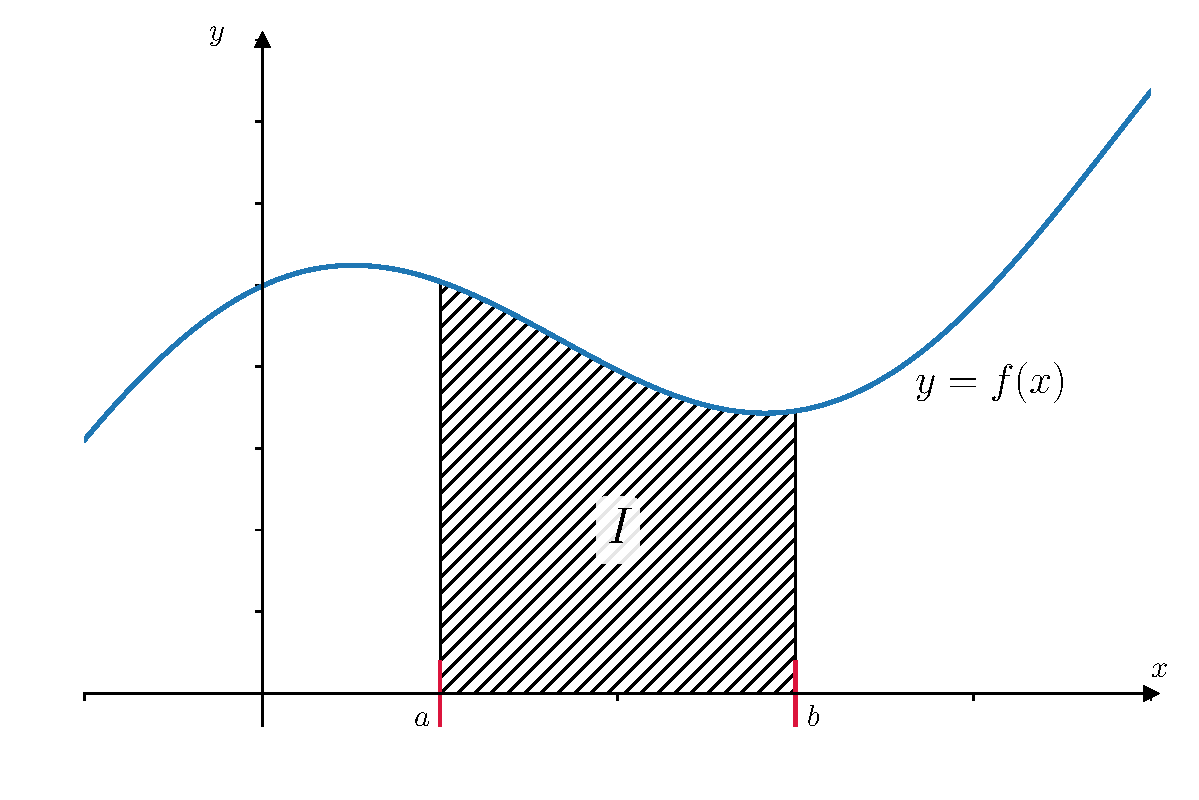
\includegraphics[width=0.6\textwidth]{figures/ch5_integration.pdf} 
	  \caption{.} \label{fig:ch5_integration}
	\end{center}
\end{figure}

\subsection{Riemann Sums}
Riemann sums approximate the integral with rectangular subdivisions. We divide the interval $[a,b]$ into $n$ equally spaced subdivisions. Denote the spacing $\Delta x = (b-a)/n$ so that the boundaries of the rectangles lie at $x_k = a + k\Delta x$ for $k=0,1,2,\dots,n$.

The left Riemann sum defines the heights of the rectangles with the function \textit{as the height at their left sides}. This gives  \\

\noindent \fbox{\begin{minipage}{\linewidth}
\underline{\textbf{Left Riemann sum for approximating an integral}}
\begin{align*}
\int_a^b f(x) dx \sim \sum_{k=0}^{n-1} f(x_k) \Delta x
\end{align*}
\end{minipage}} \\

\noindent Note the upper bound of the sum going to $n-1$, because the last rectangle will use the function at $x = b-\Delta x$ as its height. This integral approximation is represented below, for a choice of 4 subdivisions
\begin{figure}[H]
	\begin{center}
	\includegraphics[width=0.6\textwidth]{figures/ch5_riemann_left.pdf} 
	  \caption{Left Riemann sum with 4 subdivisions.} \label{fig:ch5_riemann_left}
	\end{center}
\end{figure}


The right Riemann sum defines the heights of the rectangles with the function \textit{as the height at their right sides}. This gives  \\

\noindent \fbox{\begin{minipage}{\linewidth}
\underline{\textbf{Right Riemann sum for approximating an integral}}
\begin{align*}
\int_a^b f(x) dx \sim \sum_{k=1}^{n} f(x_k) \Delta x
\end{align*}
\end{minipage}} \\
\noindent Note the sum indices going from 1 to $n$, because the first rectangle will use the function at $x = a+\Delta x$ as its height. This integral approximation is represented below, for a choice of 3 subdivisions
\begin{figure}[H]
	\begin{center}
	\includegraphics[width=0.6\textwidth]{figures/ch5_riemann_right.pdf} 
	  \caption{Left Riemann sum with 3 subdivisions.} \label{fig:ch5_riemann_right}
	\end{center}
\end{figure}

The midpoint Riemann sum defines the heights of the rectangles with the function \textit{as the height at their centres}. This gives  \\

\noindent \fbox{\begin{minipage}{\linewidth}
\underline{\textbf{Midpoint Riemann sum for approximating an integral}}
\begin{align*}
\int_a^b f(x) dx \sim \sum_{k=0}^{n-1} f\left( \frac{x_k+x_{k+1}}{2} \right) \Delta x
\end{align*}
\end{minipage}} \\
\noindent Note the sum indices going from 1 to $n$, because the first rectangle will use the function at $x = a+\Delta x$ as its height. This integral approximation is represented below, for a choice of 4 subdivisions
\begin{figure}[H]
	\begin{center}
	\includegraphics[width=0.6\textwidth]{figures/ch5_riemann_mid.pdf} 
	  \caption{Left Riemann sum with 3 subdivisions.} \label{fig:ch5_riemann_mid}
	\end{center}
\end{figure}


\subsection{Newton-Cotes methods}
The method we will use is to first estimate $f(x)$ with the Lagrangian interpolation polynomial, $p_n(x)$, and integrate that instead. So we have the approximation for the integral
\begin{align*}
I \sim \int_a^b p_n(x) dx.
\end{align*}
Figure~\ref{fig:ch5_lagrangian} shows the general schema, where we interpolate $f(x)$ using $n+1$ evenly spaced points on $[a,b]$ (including the end points).
\begin{figure}[H]
	\begin{center}
	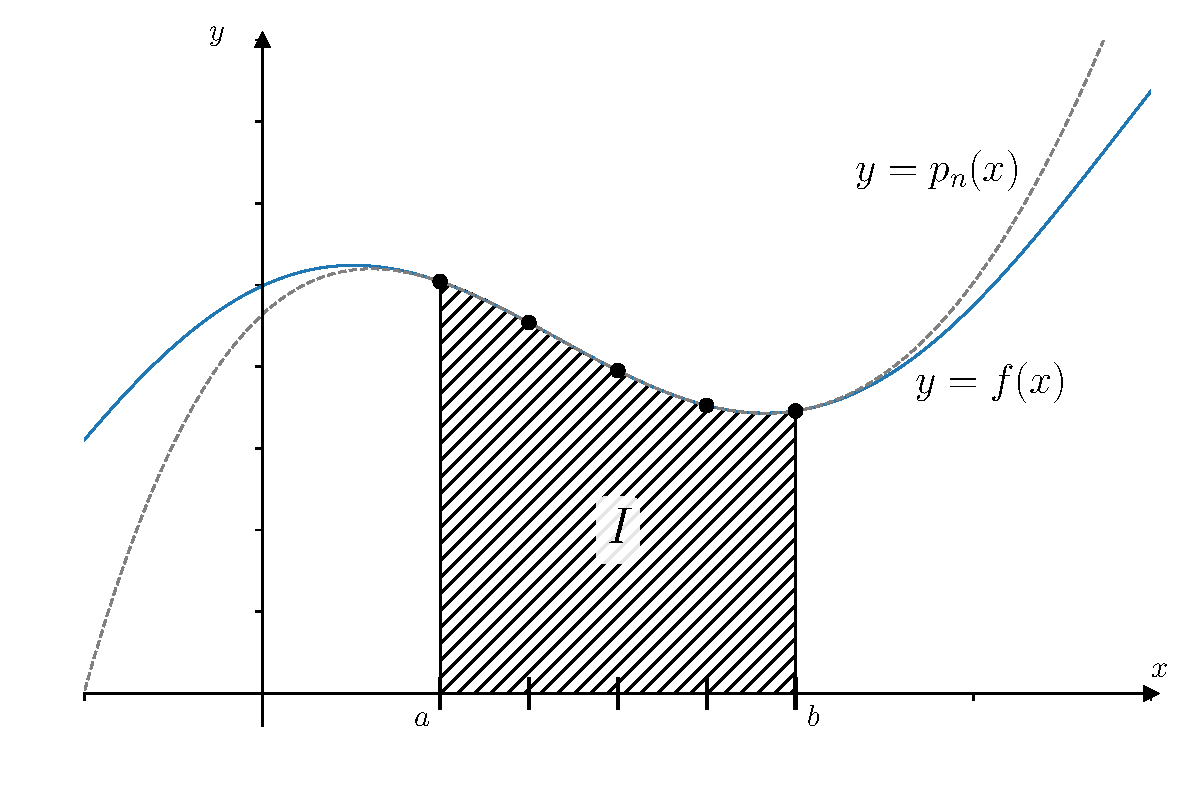
\includegraphics[width=0.6\textwidth]{figures/ch5_lagrangian.pdf} 
	  \caption{Area under a Lagrange polynomial approximation of the function $f(x)$.} \label{fig:ch5_lagrangian}
	\end{center}
\end{figure}

Recall from Chapter~\ref{ch:polynomial} that the interpolation polynomial through $n+1$ points is given by a sum over the $y$ values of the interpolation points multiplied by Lagrange basis polynomials
\begin{align*}
p(x)  = \sum_{k=0}^n y_k L_k(x) = \sum_{k=0}^n y_k \prod_{i\neq k} \frac{x-x_i}{x_k-x_i}.
\end{align*}
Since the interpolation points are given by a known function, we can set $y_k=f(x_k)$. The even spacing on $[a,b]$ also gives us the expressions for the $x$ values of the interpolation points
\begin{align*}
x_k = a + k\frac{b-a}{n}, \quad k=0,1,2,\dots,n.
\end{align*}
So the integral is approximated by
\begin{align*}
I &\sim \int_a^b \sum_{k=0}^n f(x_k) L_k(x) dx \\
&=  \sum_{k=0}^n f(x_k) \int_a^b L_k(x) dx \\
&=  \sum_{k=0}^n f(x_k) w_k
\end{align*}
where we have introduced the ``quadrature weights''
\begin{align*}
w_k = \int_a^b L_k(x) dx.
\end{align*}
This formalism of approximating an integral with evenly spaced interpolation points gives a family of formulae for different number of interpolation points, $n+1$, called \textit{Newton-Cotes formulae}. In this chapter we'll only look at $n=1$ and $n=2$, which give rise to the Trapezium and Simpson's rules, respectively.

\subsection{Trapezium rule}
If we choose $n=1$, then we interpolate the function with $n+1=2$ points. These are merely the endpoints of the interval, $x_0=a$ and $x_1=b$. Interpolating with a polynomial of degree $n=1$ means a straight line connecting these two points. This integration approximation is graphed in figure~\ref{fig:ch5_trapezium}.
\begin{figure}[H]
	\begin{center}
	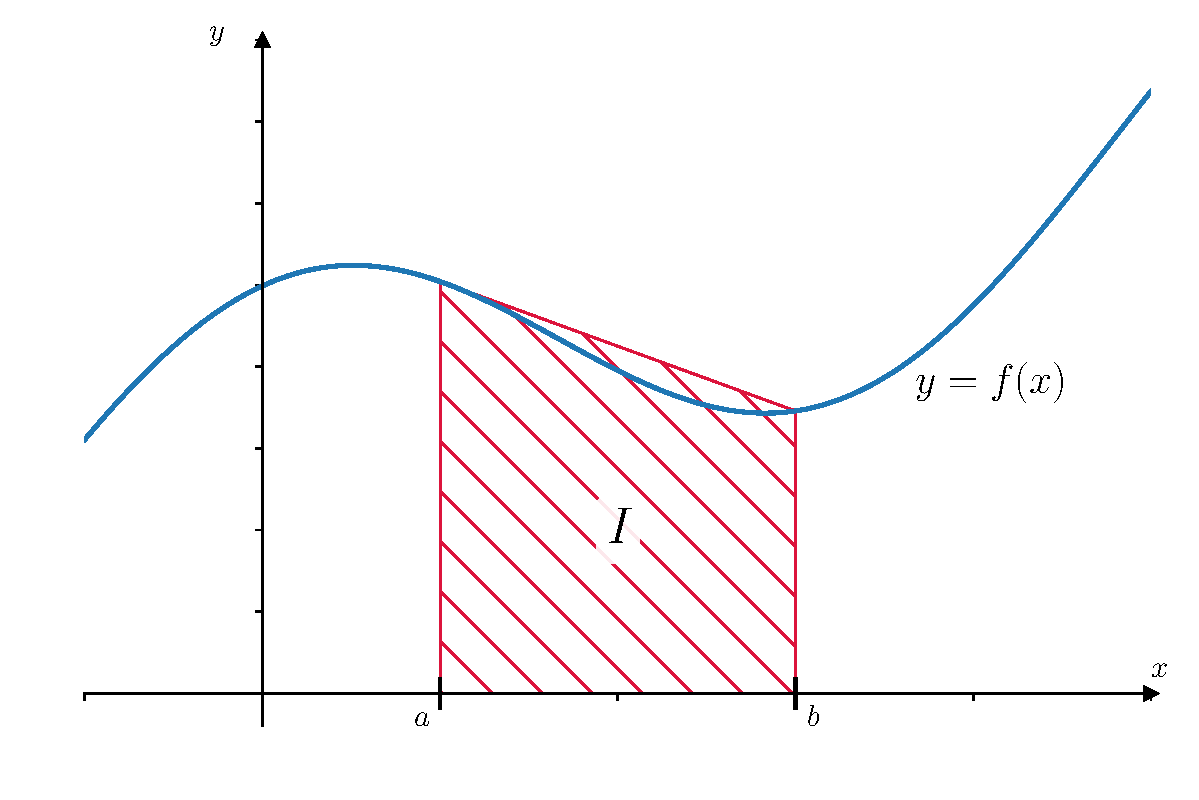
\includegraphics[width=0.6\textwidth]{figures/ch5_trapezium.pdf} 
	  \caption{Trapezium rule integral approximation.} \label{fig:ch5_trapezium}
	\end{center}
\end{figure}
The Newton-Cotes formula for $n=1$ is then
\begin{align*}
I \sim f(a) w_0 + f(b) w_1.
\end{align*}
Let's derive expressions for the quadrature weights. The zeroth weight is
\begin{align*}
w_0 &= \int_a^b L_0(x) dx, \quad \text{and } L_0 = \frac{x-b}{a-b} \\
 &= \frac{1}{a-b} \left. \left(\frac{x^2}{2} - bx \right) \right|_a^b \\
 &= \frac{1}{a-b} \left( -\frac{b^2}{2} - \frac{a^2}{2} + ba \right) \\
 &= -\frac{1}{2(a-b)} \left( a^2 - 2ab + b^2 \right) \\
 &= -\frac{1}{2(a-b)} \left( a - b \right)^2 \\
 &= \frac{b - a}{2}
\end{align*}
and similarly the first weight is
\begin{align*}
w_1 &= \int_a^b L_1(x) dx, \quad \text{and } L_1 = \frac{x-a}{b-a} \\
 &= \frac{1}{b-a} \left. \left(\frac{x^2}{2} - ax \right) \right|_a^b \\
 &= \frac{1}{2(b-a)} \left( b - a \right)^2 \\
 &= \frac{b - a}{2}.
\end{align*}
The two weights are the same! Hence we have  \\

\noindent \fbox{\begin{minipage}{\linewidth}
\underline{\textbf{Trapezium rule for approximating an integral}}
\begin{align}
\int_a^b f(x)dx \sim \frac{b-a}{2}\left(f(a) + f(b) \right) 
\end{align}
\end{minipage}} \\

\noindent With a small rearrangement we can get an alternative geometric interpretation of this rule
\begin{align*}
I \sim \underbrace{\frac{f(a) + f(b)}{2}}_\text{average height in the range} \overbrace{\left(b-a \right)}^\text{size of range}.
\end{align*}
This is simply the formula for the area of the rectangle shown below, with height equal to the average height of the function in the integration interval $[a,b]$.

\begin{figure}[H]
	\begin{center}
	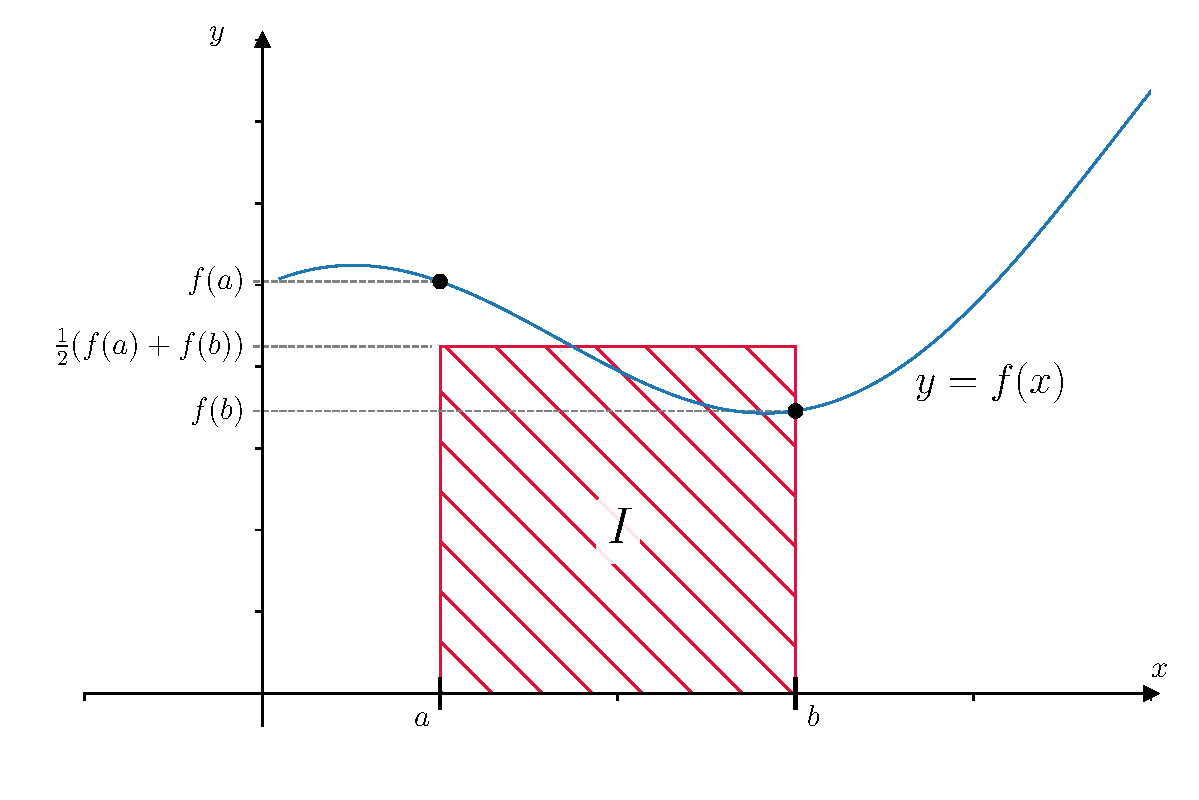
\includegraphics[width=0.6\textwidth]{figures/ch5_trapezium_alternative.pdf} 
	  \caption{Trapezium rule interpretion.} \label{fig:ch5_trapezium_alternative}
	\end{center}
\end{figure}


%%%%%%%%%%%%%%%%%%%%%%%%%%%%%%%%%%%%%%%%%%%%%%%
%%%%%%%%%%% EXAMPLE TRAPEZIUM RULE %%%%%%%%%%%%
\exemple{\upline}
{
Integrate $f(x)=e^x$ from 0 to 4 using the Trapezium rule with two (equal-sized) subdivisions.

\noindent The two subdivisions are the intervals $[0,2]$ and $[2,4]$. The areas are sketched out below
\begin{figure}[H]
	\begin{center}
	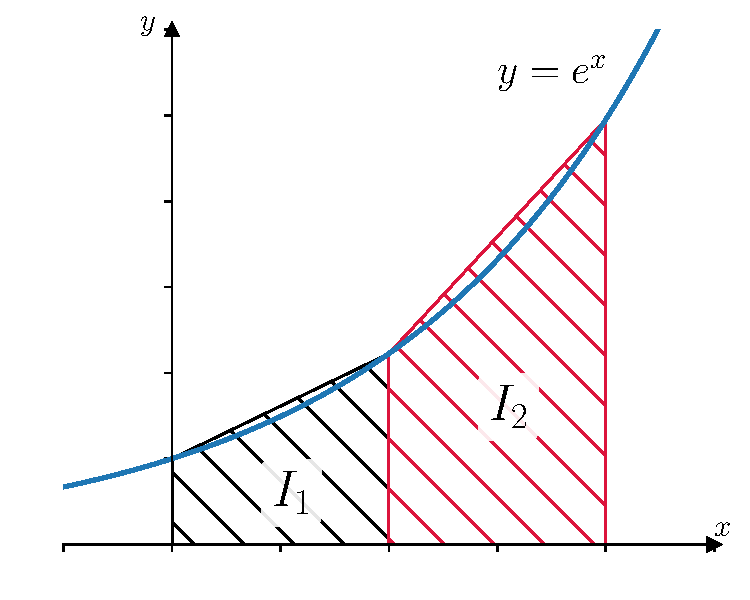
\includegraphics[width=0.6\textwidth]{figures/ch5_trapezium_example.pdf} 
	  \caption{Trapezium rule with two equal subdivisions.} \label{fig:ch5_trapezium_example}
	\end{center}
\end{figure}
The two integrals are then
\begin{align*}
&\int_0^2 e^x dx \sim I_1 = \frac{2-0}{2} \left(f(0) + f(2) \right) = e^0 + e^2 = 1 + e^2 \\
&\int_2^4 e^x dx \sim I_2 = \frac{4-2}{2} \left(f(2) + f(4) \right) = e^2 + e^4.
\end{align*}
Therefore the approximation of the total integral is just the addition of these two parts
\begin{align*}
\int_0^4 e^x dx \sim 1 + 2e^2 + e^4 \sim 70.4.
\end{align*}
}{\downline}
%%%%%%%%%%%%%%%%%%%%%%%%%%%%%%%%%%%%%%%%%%%%%%%
%%%%%%%%%%%%%%%%%%%%%%%%%%%%%%%%%%%%%%%%%%%%%%%

\subsection{Simpson's rule}
Now we choose $n=2$, so we interpolate the function with $n+1=3$ points. These 3 points are the endpoints of the interval and the midpoint, $x_0=a$, $x_1=(a+b)/2$, and $x_2=b$. Interpolating with a polynomial of degree $n=2$ means a quadratic through the points. This integration approximation is graphed in figure~\ref{fig:ch5_simpsons}.
\begin{figure}[H]
	\begin{center}
	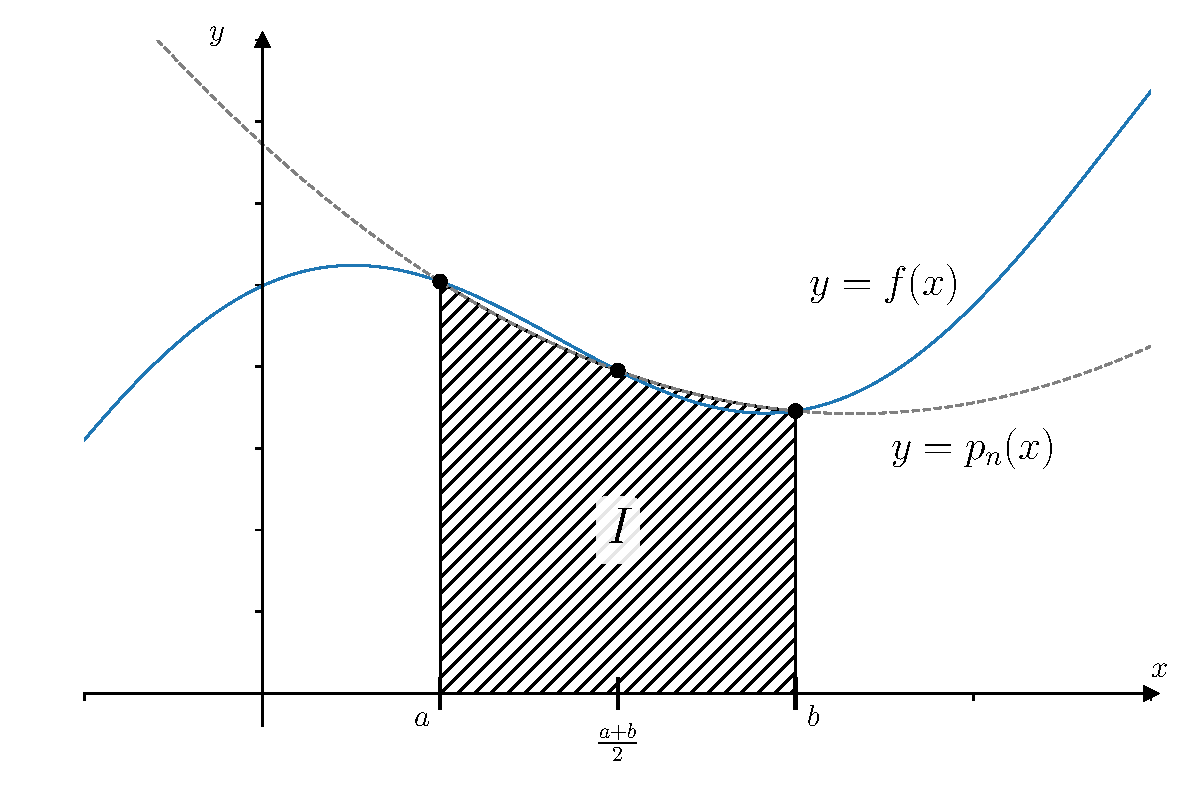
\includegraphics[width=0.6\textwidth]{figures/ch5_simpsons.pdf} 
	  \caption{Simpson's rule.} \label{fig:ch5_simpsons}
	\end{center}
\end{figure}
The Newton-Cotes formula for $n=2$ is then
\begin{align*}
I \sim f(a) w_0 + f(\frac{a+b}{2}) w_1 + f(b) w_2.
\end{align*}
Let's derive expressions for the quadrature weights. Sometimes it will be convenient to use the midpoint $m=(a+b)/2$. Then the zeroth weight is
\begin{align*}
w_0 &= \int_a^b L_0(x) dx, \quad \text{and } L_0 = \frac{(x-m)(x-b)}{(a-m)(a-b)}.
\end{align*}
Let's integrate just the numerator for now
\begin{align*}
\int_a^b (x-m)(x-b) dx &= \left.\left( \frac{x^3}{3} - \frac{m+b}{2}x^2 + mbx \right) \right|_a^b \\
&=  \frac{b^3}{3} - \frac{m+b}{2}b^2 + mb^2  -  \frac{a^3}{3} + \frac{m+b}{2}a^2 - mba  \\
&=  \frac{b^3}{3} - \frac{ab^2}{4}  - \frac{b^3}{4} - \frac{b^3}{2} +  \frac{ab^2}{2} +  \frac{b^3}{2} -  \frac{a^3}{3} + \frac{a^3}{4} + \frac{ba^2}{4} + \frac{ba^2}{2} -  \frac{ba^2+ab^2}{2} \\
&= \frac{1}{12}\left(b^3 - 3ab^2 + 3ba^2 - a^3\right) \\
&= \frac{1}{12}\left(b - a\right)^3.
\end{align*}
The weight is then
\begin{align*}
w_0 &= \frac{1}{12} \frac{\left(b - a\right)^3}{(a-m)(a-b)} \\
 &= \frac{1}{12} \frac{\left(b - a\right)^2}{m-a}
\end{align*}
This denominator is
\begin{align*}
m-a = \frac{a+b}{2}-a = \frac{b-a}{2}
\end{align*}
and so the final expression for the weight is
\begin{align*}
w_0 = \frac{b-a}{6}.
\end{align*}
It's not so difficult to show that the other two weights are
\begin{align*}
w_1 &= \frac{4}{6}\left(b-a\right), \\
w_2 &= \frac{b-a}{6}.
\end{align*}
And so we have \\

\noindent \fbox{\begin{minipage}{\linewidth}
\underline{\textbf{Simpson's rule for approximating an integral}}
\begin{align}
\int_a^b f(x)dx \sim \frac{b-a}{6}\left(f(a) + 4f\left(\frac{a+b}{2}\right)+ f(b) \right)
\end{align}
\end{minipage}} \\

\noindent Sometimes we use the distance between the interpolation points, $h=(b-a)/2$, and then Simpson's rule is written
\begin{align*}
\int_a^b f(x)dx \sim \frac{h}{3}\left(f(a) + 4f\left(\frac{a+b}{2}\right)+ f(b) \right).
\end{align*}
from which we get the alternative name \textit{Simpson's 1/3 rule}. Be very careful here: $h$ is the distance between interpolation points (half the integration interval).

%%%%%%%%%%%%%%%%%%%%%%%%%%%%%%%%%%%%%%%%%%%%%%%
%%%%%%%%%%% EXAMPLE SIMPSON'S RULE %%%%%%%%%%%%
\exemple{\upline}
{
Integrate $f(x)=e^x$ from 0 to 4 using Simpson's rule with two (equal-sized) subdivisions.

\noindent The two subdivisions are the intervals $[0,2]$ and $[2,4]$. The areas are sketched out below
\begin{figure}[H]
	\begin{center}
	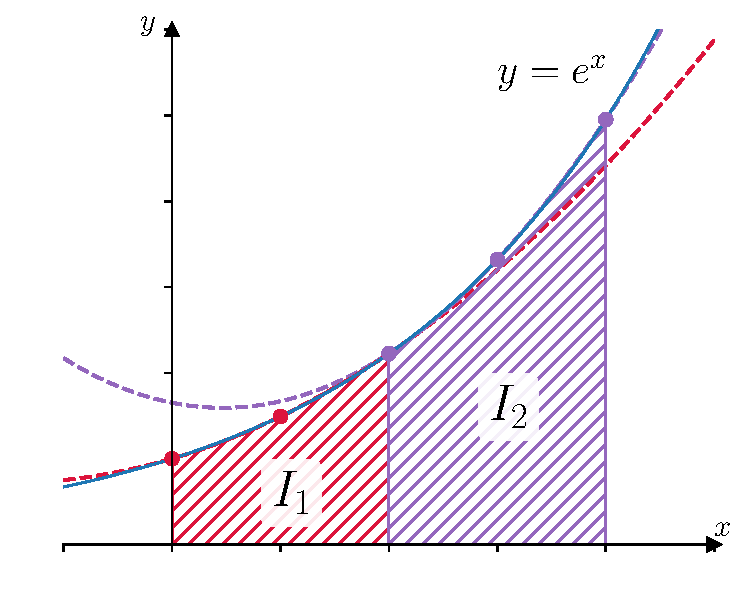
\includegraphics[width=0.6\textwidth]{figures/ch5_simpsons_example.pdf} 
	  \caption{Simpson's rule with two equal subdivisions.} \label{fig:ch5_simpsons_example}
	\end{center}
\end{figure}
\noindent The two integrals are then
\begin{align*}
&\int_0^2 e^x dx \sim I_1 = \frac{2-0}{6} \left(f(0) + 4f(1) + f(2) \right) = \frac{1}{3}\left(1 + 4e + e^2\right) \\
&\int_2^4 e^x dx \sim I_2 = \frac{4-2}{6} \left(f(2) + 4f(3) + f(4) \right) = \frac{1}{3}\left(e^2 + 4e^3 + e^4\right).
\end{align*}
Therefore the approximation of the total integral is just the addition of these two parts
\begin{align*}
\int_0^4 e^x dx \sim \frac{1}{3}\left(1 + 4e + 2e^2 + 4e^3 + e^4\right) \sim 53.9.
\end{align*}
This integral can be solved analytically for comparison
\begin{align*}
\int_0^4 e^x dx = \left. e^x\right|_0^4 = e^4 - 1 \sim 53.6.
\end{align*}
So the Simpson's rule approximation is much better than the Trapezium rule result.
}{\downline}
%%%%%%%%%%%%%%%%%%%%%%%%%%%%%%%%%%%%%%%%%%%%%%%
%%%%%%%%%%%%%%%%%%%%%%%%%%%%%%%%%%%%%%%%%%%%%%%

\subsubsection{Composite Simpson's rule}

It's not necessarily the case that increasing the number of interpolation points increases the accuracy of the approximation. Consider the integral
\begin{align*}
\int_{-5}^5 \frac{1}{1+x^2} dx.
\end{align*}
Applying Newton-Cotes formulae to this integral with increasing $n$ does not converge on the exact solution, and in fact eventually gives values that increase without bound. It is generally better to stick with Simpson's rule, but to increase the number of subdivisions, as shown below:
\begin{figure}[H]
	\begin{center}
	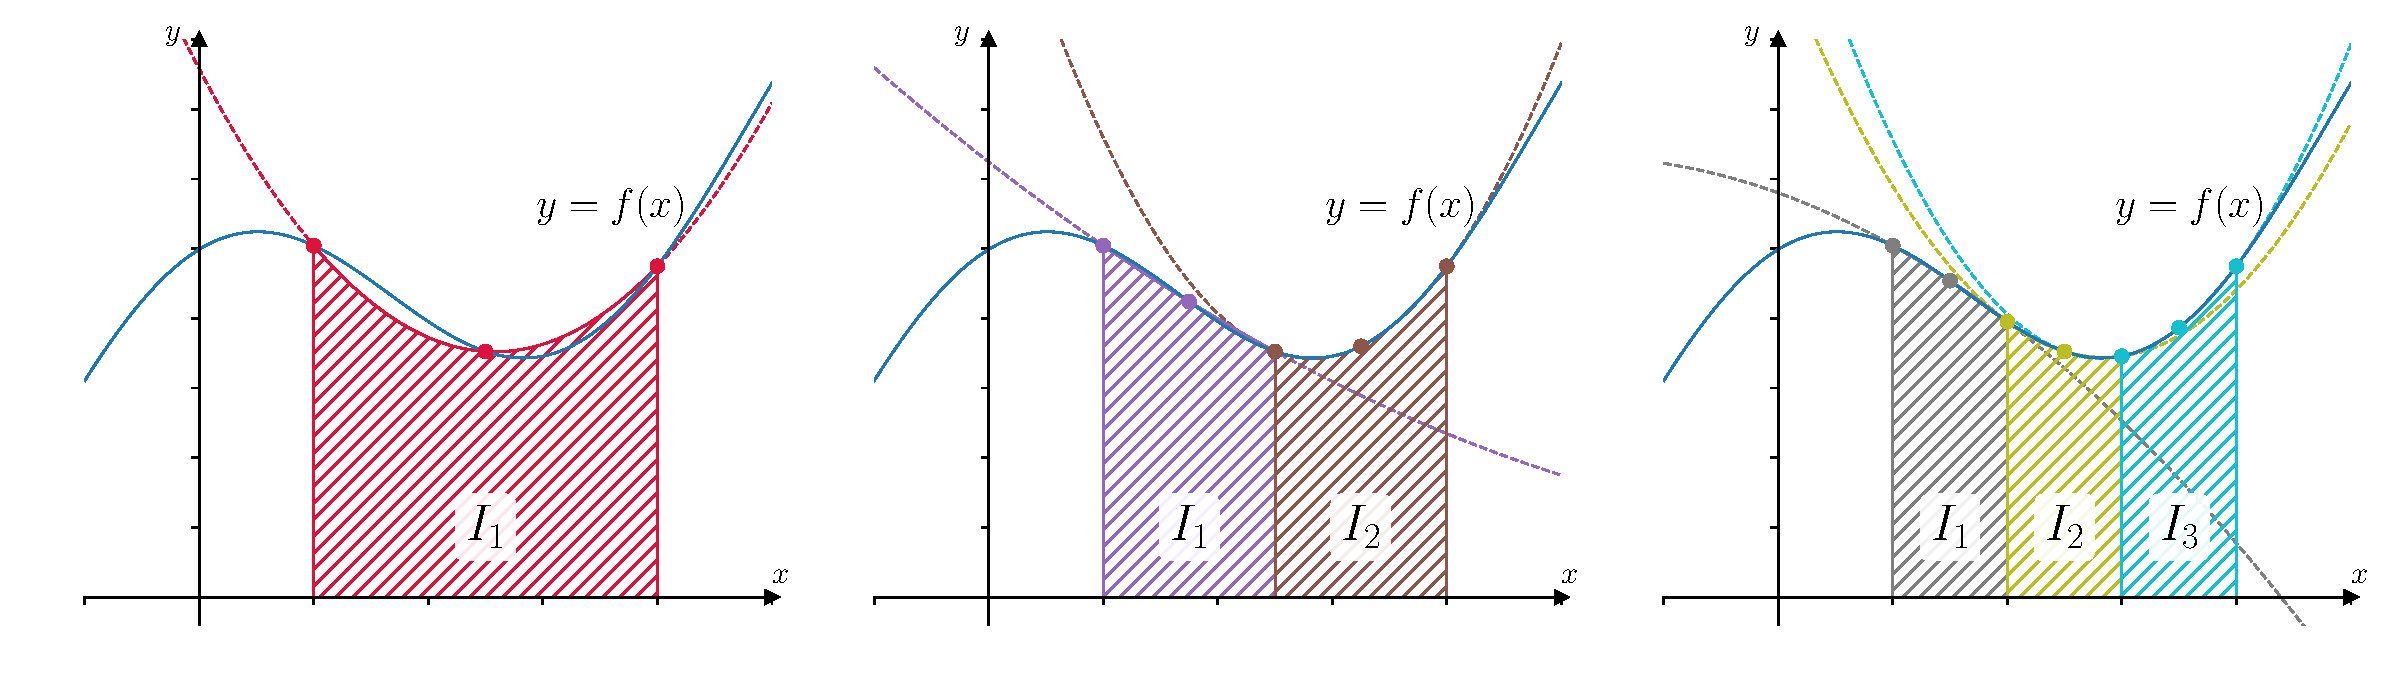
\includegraphics[width=\textwidth]{figures/ch5_simpsons_refinement.pdf} 
	  \caption{Simpson's rule using 1, 2 or 3 subdivisions.} \label{fig:ch5_simpsons_refinement}
	\end{center}
\end{figure}

\noindent The total integral approximation is now formalised as a summation
\begin{align*}
\int_a^b f(x)dx \sim \sum_k I_k
\end{align*}
where the $I_k$ are each applications of Simpson's rule. We study here how this composite rule results in a simple formula. 

Consider dividing an interval $[a,b]$ into $n$ equal sized subdivisions, so that $k=1,2,\dots,n$. We want to apply Simpson's rule to each subdivision, which has width $(b-a)/n$. Since $h$ is half the size of these subdivisions, we have $h = (b-a)/2n$. In each subdivision, the interpolation points are separated by $h$, and so the areas are
\begin{align*}
I_1 &= \frac{h}{3}\left( f(a) + 4f(a+h) + f(a+2h) \right) \\
I_2 &= \frac{h}{3}\left( f(a+2h) + 4f(a+3h) + f(a+4h) \right) \\
I_3 &= \frac{h}{3}\left( f(a+4h) + 4f(a+5h) + f(a+6h) \right) \\
&\vdots \\
I_n &= \frac{h}{3}\left( f(a+(2n-2)h) + 4f(a+(2n-1)h) + f(a+2nh) \right)
\end{align*}
We quickly make sure this is right by checking that the last term is what we expect:
\begin{align*}
I_n &= \frac{h}{3}\left( f(b-2h) + 4f(b-h) + f(b) \right)
\end{align*}
We should recover this last interval when we replace $n$ with $n = (b-a)/2h$:
\begin{align*}
I_n &= \frac{h}{3}\left( f(a+(2n-2)h) + 4f(a+(2n-1)h) + f(a+2nh) \right) \\
&= \frac{h}{3}\left( f(a+(2\frac{b-a}{2h}-2)h) + 4f(a+(2\frac{b-a}{2h}-1)h) + f(a+2\frac{b-a}{2h}h) \right) \\
&= \frac{h}{3}\left( f(a+b-a-2h) + 4f(a+b-a -h)) + f(a+b-a) \right) \\
&= \frac{h}{3}\left( f(b-2h) + 4f(b-h)) + f(b) \right)
\end{align*}
Good it works. Now if we add all the subdivision Simpson rule areas together you should see that the 3rd term in one expression is the 1st term in the next. These can be collected
\begin{align*}
\int_a^b f(x)dx \sim \frac{h}{3}\left(f(a) + 4f(a+h) + 2f(a+2h)  + 4f(a+3h) + 2f(a+4h)  + 4f(a+5h) + \cdots + f(b) \right)
\end{align*}
The terms multiplied by 4 are always of the form $a+Xh$ for odd $X$, while the terms multiplied by 2 are all of the form $a+Yh$ for even $Y$. This gives the following formula. \\

\noindent \fbox{\begin{minipage}{\linewidth}
\underline{\textbf{Composite Simpson's rule for approximating an integral}} \\

For a function $f(x)$ that is continuous on the interval $[a,b]$:
\begin{align}
\int_a^b f(x)dx \sim \frac{h}{3}\left(f(a) + 4\sum_{k=1}^n f\left(a+(2k-1)h\right) + 2\sum_{k=1}^{n-1} f\left(a+2kh\right) + f(b) \right)
\end{align}
where
\begin{align*}
h = \frac{b-a}{2n}.
\end{align*}
Alternatively:
\begin{align}
\int_a^b f(x)dx \sim \frac{h}{3}\left(f(a) + 4\sum_{k=1}^n f\left(x_{2k-1}\right) + 2\sum_{k=1}^{n-1} f\left(x_{2k}\right) + f(b) \right)
\end{align}
where
\begin{align*}
\quad x_k = a + k h
\end{align*}
\end{minipage}} \\

\subsection{Degree of precision}

For an integration approximation scheme, the degree of precision of is the largest $k$ such that the integration scheme applied to $x^k$ gives the exact answer for $\int x^k \, dx$ which is of course $x^{k+1}/(k+1)$. That is, a scheme with degree of precision $k$ will be exact when applied to
\begin{align*}
1 \quad x \quad x^2 \quad \cdots \quad x^k
\end{align*}
but will fail to give the exact value when applied to $x^{k+1}$.

\exemple{\upline}{
Find the degree of precision for the Trapezium rule and for Simpson's rule. \\

\noindent For the Trapezium rule, when $f(x)=x^0$ we have
\begin{align*}
\int_a^b 1 dx \sim \frac{b-a}{2}\left(f(a) + f(b) \right) &= \frac{b-a}{2}\left(1 + 1 \right) \\
&= b-a \\
&= \left. x \right|_a^b
\end{align*}
This is exact so we check the next power. For $f(x)=x^1$ we have
\begin{align*}
\int_a^b x dx &\sim  \frac{b-a}{2}\left(a + b \right) \\
&= \frac{b^2-a^2}{2} \\
&= \left.\frac{x^2}{2} \right|_a^b
\end{align*}
This is exact so we check the next power. For $f(x)=x^2$ we have
\begin{align*}
\int_a^b x^2 dx &\sim \frac{b-a}{2}\left(a^2 + b^2 \right) \\
&= \frac{b^3 + ba^2 -ab^2 -a^3}{2} \\
& \neq \left.\frac{x^3}{3} \right|_a^b
\end{align*}
As $k=1$ is the highest power for which the Trapezium rule gave the exact result, the degree of precision is 1. \\

\noindent For Simpson's rule, when $f(x)=x^0$ we have
\begin{align*}
\int_a^b 1 dx \sim \frac{b-a}{6}\left(f(a) + 4f\left(\frac{a+b}{2}\right)+ f(b) \right)  &= \frac{b-a}{6}\left(1 + 4+ 1 \right). \\
&= b-a \\
&= \left. x \right|_a^b
\end{align*}
This is exact so we check the next power. For $f(x)=x^1$ we have
\begin{align*}
\int_a^b x dx &\sim \frac{b-a}{6}\left(a + 4\left(\frac{a+b}{2}\right)+ b \right)  \\
&= \frac{b-a}{6}\left(3a + 3b \right) \\
&= \frac{b^2-a^2}{2}\\
&= \left.\frac{x^2}{2} \right|_a^b
\end{align*}
This is exact so we check the next power. For $f(x)=x^2$ we have
\begin{align*}
\int_a^b x^2 dx &\sim \frac{b-a}{6}\left(a^2 + 4\left(\frac{a+b}{2}\right)^2+ b^2 \right)  \\
&= \frac{b-a}{6}\left(a^2 + 4\left(\frac{a^2+2ab + b^2}{4}\right)+ b^2 \right)  \\
&= \frac{b-a}{3}\left(a^2 +ab + b^2 \right) \\
&= \frac{b^3-a^3}{3} \\
&= \left.\frac{x^3}{3} \right|_a^b
\end{align*}
This is exact so we check the next power. For $f(x)=x^3$ we have
\begin{align*}
\int_a^b x^3 dx &\sim \frac{b-a}{6}\left(a^3 + 4\left(\frac{a+b}{2}\right)^3+ b^3 \right)  \\
&= \frac{b-a}{6}\left(a^3 + 4\left(\frac{a^3+3a^2b + 3ab^2  + b^3}{8}\right)+ b^3 \right)  \\
&= \frac{b-a}{6}\left(\frac{3}{2}a^3 + \frac{3}{2}a^2b + \frac{3}{2}ab^2+ \frac{3}{2}b^3 \right)  \\
&= \frac{b^4 - a^4}{4} \\
&= \left.\frac{x^4}{4} \right|_a^b
\end{align*}
This is exact so we check the next power. For $f(x)=x^4$ we have
\begin{align*}
\int_a^b x^4 dx &\sim \frac{b-a}{6}\left(a^4 + 4\left(\frac{a+b}{2}\right)^4+ b^4 \right)  \\
&= \frac{b-a}{6}\left(a^4 + 4\left(\frac{a^4 + 4 a^3 b + 6 a^2 b^2 + 4 a b^3  + b^4}{16}\right)+ b^4 \right)  \\
&= \frac{b-a}{24}\left(5 a^4 + 4 a^3 b + 6 a^2 b^2 + 4 a b^3  + 5 b^4 \right)  \\
&= \frac{5 b^5 + a^4 b - 2 a^3 b^2 + 2 a^2 b^3 - a b^4 - 5 a^5}{24}  \\
& \neq \left.\frac{x^5}{5} \right|_a^b
\end{align*}
As $k=3$ is the highest power for which Simpson's rule gave the exact result, the degree of precision is 3.
}{\downline}


%%%%%%%%%%%%%%%%%%%%%%%%%%%%%%%%%%%%%%%%%%
%%%%%%%%%%%%%%%%%%%%%%%%%%%%%%%%%%%%%%%%%%
%%%%%%%%%%%%%%%%%%%%%%%%%%%%%%%%%%%%%%%%%%








%%%%%%%%%%%%%%%%%%%%%%%%%%%%%%%%%%%%%%%%%%
%%%%%%%%%%%%%%%%%%%%%%%%%%%%%%%%%%%%%%%%%%
%%%%%%%%%%%%%%%%%%%%%%%%%%%%%%%%%%%%%%%%%%
%%%%%%%%%%%  DIFFERENTIATION %%%%%%%%%%%%%
%%%%%%%%%%%%%%%%%%%%%%%%%%%%%%%%%%%%%%%%%%
%%%%%%%%%%%%%%%%%%%%%%%%%%%%%%%%%%%%%%%%%%
%%%%%%%%%%%%%%%%%%%%%%%%%%%%%%%%%%%%%%%%%%
\section{Numerical differentiation}
The goal is to find the slope of some known function, $f(x)$, at a point $x=x_k$, giving just 1 real value
\begin{align*}
m=f'(x_k)
\end{align*}
as shown below.
\begin{figure}[H]
	\begin{center}
	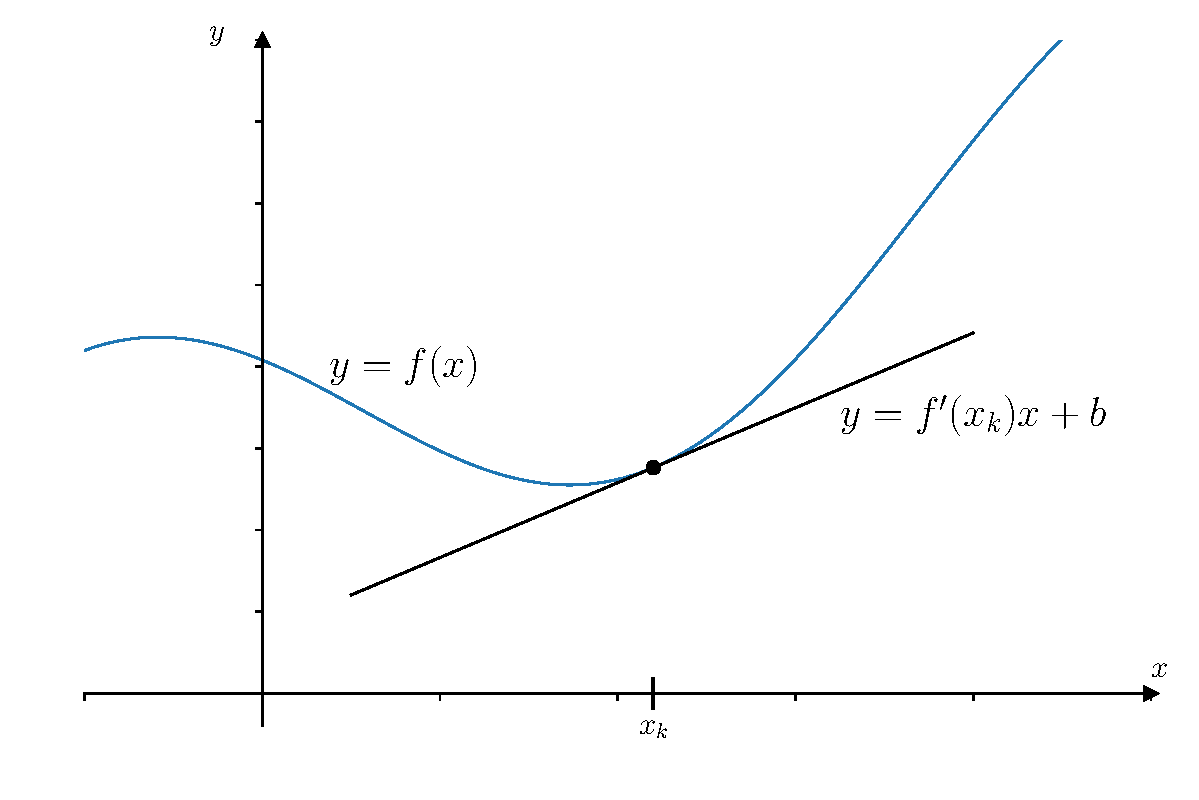
\includegraphics[width=0.6\textwidth]{figures/ch5_derivative.pdf} 
	  \caption{.} \label{fig:ch5_derivative}
	\end{center}
\end{figure}

The method will be just like with integration, we first estimate the function with a Lagrange polynomial, $p_n(x)$ and differentiate that instead (and then evaluate the polynomial at $x_k$)! That is,
\begin{align*}
f'(x_k) \sim \frac{d p_n}{dx}(x_k).
\end{align*}
We will here look at only $n=1$, which gives the forward and backward finite difference schemes, and $n=2$, which gives the centred finite difference scheme.

\subsection{Forward and backward finite difference}
For $n=1$, we need $n+1=2$ points of interpolation. Of course $x=x_k$ will be one of the points, but we have a free choice for the second point. If we choose the second point to be greater than $x_k$ we get the forward finite difference scheme, whereas if we choose it to be less than $x_k$ we get the backward finite difference scheme. The two schemes are illustrated below.
\begin{figure}[H]
	\begin{center}
	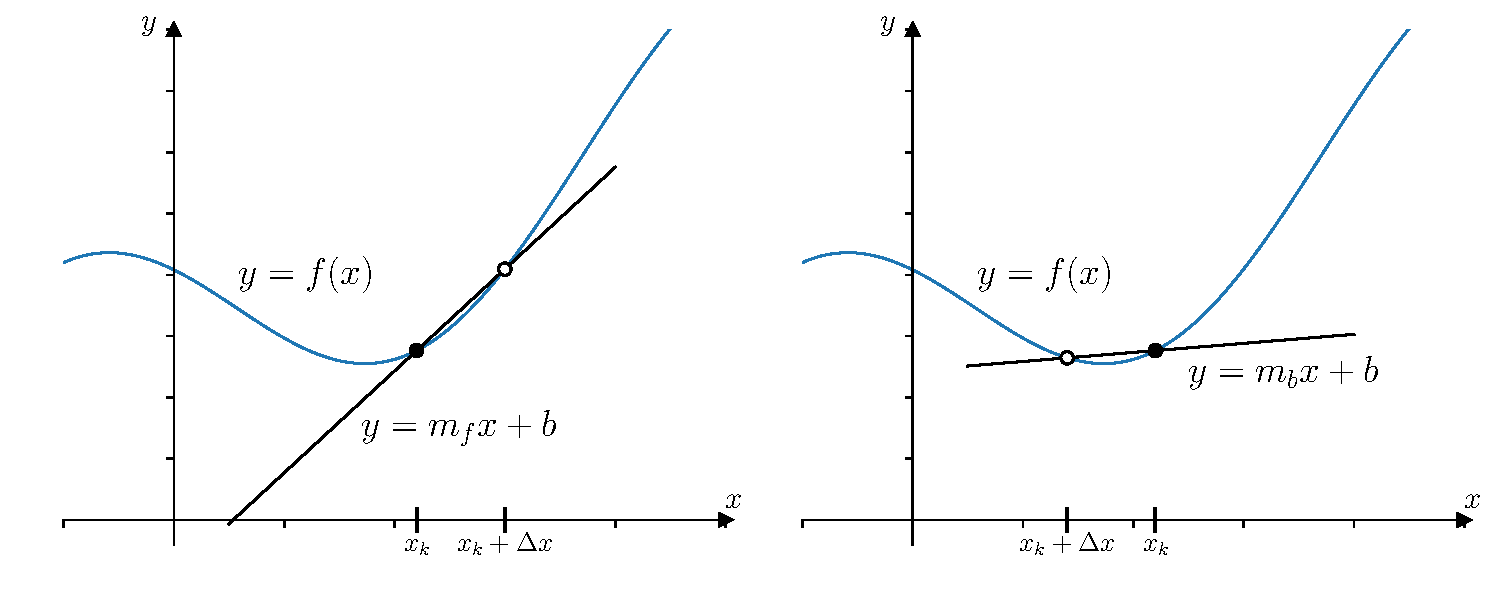
\includegraphics[width=\textwidth]{figures/ch5_forward_backward_difference.pdf} 
	  \caption{(Left) forward finite difference scheme and (right) backward finite difference scheme.} \label{fig:ch5_forward_backward_difference}
	\end{center}
\end{figure}
Consider the forward scheme, so that the interpolation positions are $x_0=x_k$ and $x_1=x_k+\Delta x$ for some small distance $\Delta x$. Then the Lagrange polynomial is given by
\begin{align*}
f(x) \sim p_1(x) = f(x_0) L_0(x) + f(x_1) L_1(x).
\end{align*}
The Lagrange basis polynomials are
\begin{align*}
L_0(x) &= \frac{x-x_1}{x_0-x_1} = \frac{x-x_k-\Delta x}{-\Delta x} \\
L_1(x) &= \frac{x-x_0}{x_1-x_0} = \frac{x-x_k}{\Delta x}.
\end{align*}
So the derivative of $f$ is approximated by
\begin{align*}
\frac{d p_1}{dx} &= f(x_0) \frac{dL_0}{dx} + f(x_1) \frac{dL_1}{dx} \\
 &= f(x_0) \frac{1}{-\Delta x} + f(x_1)\frac{1}{\Delta x} \\
 &= \frac{f(x_1)- f(x_0)}{\Delta x} \\
 &= \frac{f(x_k + \Delta x)- f(x_k)}{\Delta x}.
\end{align*}
I hope a sense of familiarity is tickling your brain right now, because this is exactly the form of the first principles definition of the derivative of a function at a point $x_k$
\begin{align*}
\frac{df}{dx}(x_k) = \lim_{\Delta x \to 0} \frac{f(x_k + \Delta x)- f(x_k)}{\Delta x}.
\end{align*}
So this scheme converges on the true derivative as $\Delta x$ becomes very small. So we have 

\vspace{0.2cm} \noindent \fbox{\begin{minipage}{\linewidth}
\underline{\textbf{Forward finite difference approximation of a derivative}}
\begin{align}
f'(x_k) \sim \frac{f(x_k + \Delta x)- f(x_k)}{\Delta x}.
\end{align}
\end{minipage}}\vspace{0.2cm} 

\noindent The formula for backward finite difference is quite straightforward (you should try to guess it before looking down)


\vspace{0.2cm} \noindent \fbox{\begin{minipage}{\linewidth}
\underline{\textbf{Backward finite difference approximation of a derivative}}
\begin{align}
f'(x_k) \sim \frac{f(x_k)- f(x_k - \Delta x)}{\Delta x}.
\end{align}
\end{minipage}}\vspace{0.2cm} 

The accuracy of these approximations can be assessed using the Taylor expansion of $f$
\begin{align*}
f(x) = \sum_{n=0}^{\infty} f^{(n)}(a)\frac{\left(x-a\right)^n}{n!}.
\end{align*}
We replace $x$ with $x+\Delta x$ and use $a=x$
\begin{align*}
f(x+\Delta x) &= \sum_{n=0}^{\infty} f^{(n)}(x)\frac{\left(\Delta x\right)^n}{n!} \\
&= f(x) + f'(x) \Delta x + f''(x) \frac{\left( \Delta x\right)^2}{2} + \cdots
\end{align*}
Rearranging for the first derivative
\begin{align*}
f'(x) = \underbrace{\frac{f(x+\Delta x) - f(x)}{\Delta x}}_{\text{forward finite difference scheme}} - \underbrace{f''(x) \frac{\Delta x}{2}}_\text{largest error term} - \cdots
\end{align*}
So we see that the largest error term is controlled by the second derivative (because further derivatives get multiplied by increasing powers of $\Delta x$, which becomes very small). This makes sense. Consider the graphs of the two functions below.
\begin{figure}[H]
	\begin{center}
	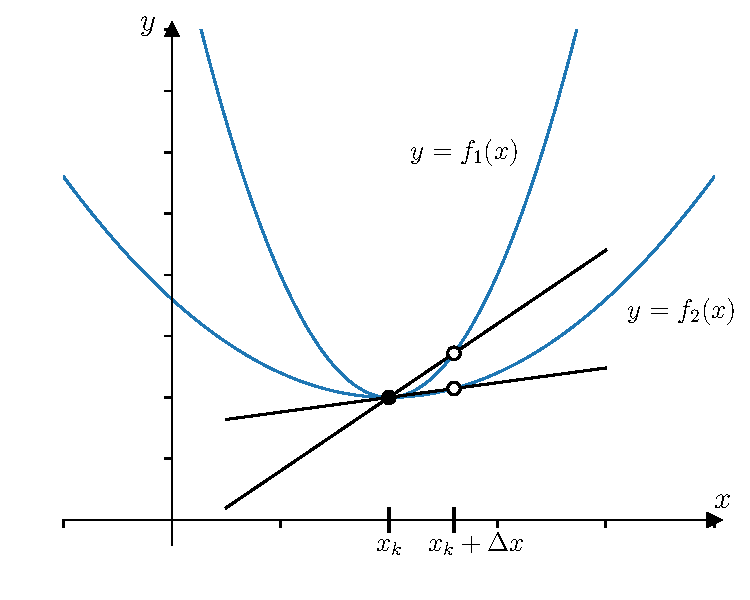
\includegraphics[width=0.8\textwidth]{figures/ch5_forward_difference_2nd_deriv.pdf} 
	  \caption{Two functions $f_1(x)$ and $f_2(x)$ with same first derivatives $f_1'(x_k)=f_2'(x_k)$ at $x=x_k$, but different second derivatives $f_1''(x_k)>f_2''(x_k)$.} \label{fig:ch5_forward_difference_2nd_deriv}
	\end{center}
\end{figure}
\noindent Both of these functions have the same slope at $x=x_k$. But the function $f_1(x)$ has a larger second derivative than $f_2(x)$ at that position. You can see that the forward finite difference approximation to the derivative at this position, despite using the same $\Delta x$, is worse for the function with larger second derivative at the position.

\exemple{\upline}{
Given the data
\begin{figure}[H]
\begin{tabular}{l|lllll}
$x$    & 4.5000   & 4.5025   & 4.5050   & 4.5075   & 4.5100 \\  \hline
$f(x)$ & 405.563  & 406.472  & 407.383  & 408.296  & 409.210
\end{tabular}
\end{figure}

\noindent Estimate estimate $f'(4.5050)$ by using forward finite difference with $\Delta x=0.0025$ and backward finite difference with $\Delta x=0.005$.

We are estimating the derivative at the position $x_k=4.5050$. For forward finite difference, $x_k+\Delta x=4.5075$. So we have
\begin{align*}
f'(4.5050) &= \frac{f(4.5075) - f(4.5050)}{0.0025} \\
&= \frac{408.296 - 407.383}{0.0025} \\
&\sim 365.200
\end{align*}

For backward finite difference with $\Delta x=0.005$ we have $x_k-\Delta x=4.5000$
\begin{align*}
f'(4.5050) &= \frac{f(4.5050) - f(4.5000)}{0.005} \\
&= \frac{407.383 - 405.563}{0.005} \\
&\sim 364.000
\end{align*}
}{\downline}





\subsection{Centred finite difference}
Now we consider $n=2$, so that we have $n+1=3$ interpolation points. The centred finite difference scheme uses the point of interest, at $x=x_k$, as one of the interpolation points, with the other two equidistant on either side, at $x=x_k \pm \Delta x$, as sketched below:
\begin{figure}[H]
	\begin{center}
	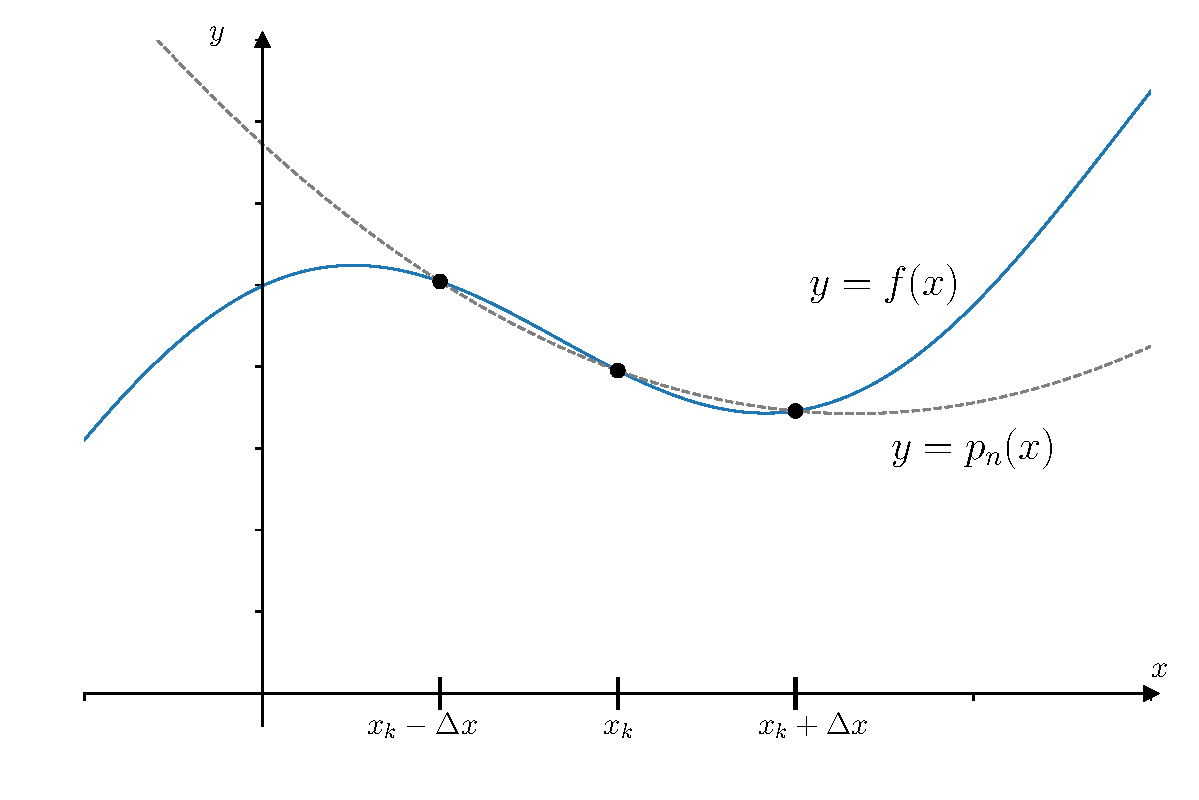
\includegraphics[width=0.6\textwidth]{figures/ch5_centred_finite_difference.pdf} 
	  \caption{Lagrange polynomial of order 2 (quadratic) used for the centred finite difference approximation to the derivative of $f(x)$ at $x=x_k$.} \label{fig:ch5_centred_finite_difference}
	\end{center}
\end{figure}
So, the Lagrange polynomial will be given by
\begin{align*}
f(x) \sim p_2(x) = f(x_k - \Delta x)L_0(x) + f(x_k)L_1(x) + f(x_k + \Delta x)L_2(x)
\end{align*}
Defining $x_0=x_k - \Delta x$, $x_1=x_k$ and  $x_2=x_k + \Delta x$, the basis polynomials are
\begin{align*}
L_0(x) &= \frac{(x-x_1)(x-x_2)}{(x_0-x_1)(x_0-x_2)} = \frac{x^2 - (x_1+x_2)x + x_1x_2}{(x_0-x_1)(x_0-x_2)} \\
%
L_1(x) &= \frac{(x-x_0)(x-x_2)}{(x_1-x_0)(x_1-x_2)} = \frac{x^2 - (x_0+x_2)x + x_0x_2}{(x_1-x_0)(x_1-x_2)} \\
%
L_2(x) &= \frac{(x-x_0)(x-x_1)}{(x_2-x_0)(x_2-x_1)} = \frac{x^2 - (x_0+x_1)x + x_0x_1}{(x_2-x_0)(x_2-x_1)}.
\end{align*}
As we will differentiate $p_2(x)$, we need the derivatives of these basis polynomials
\begin{align*}
L_0'(x) &= \frac{2x - (x_1+x_2)}{(x_0-x_1)(x_0-x_2)} = \frac{2x - 2x_k - \Delta x}{2(\Delta x)^2} \\
%
L_1'(x) &= \frac{2x - (x_0+x_2)}{(x_1-x_0)(x_1-x_2)} = \frac{2x - 2x_k}{-(\Delta x)^2}\\
%
L_2'(x) &= \frac{2x - (x_0+x_1)}{(x_2-x_0)(x_2-x_1)} = \frac{2x - 2x_k + \Delta x}{2(\Delta x)^2}.
\end{align*}
Then, we have the derivative of the Lagrange polynomial at the position $x=x_k$
\begin{align*}
\frac{dp_2}{dx}(x_k) &= f(x_k - \Delta x) L_0'(x_k) + f(x_k)L_1'(x_k) + f(x_k + \Delta x)L_2'(x_k) \\
&= \frac{-f(x_k - \Delta x) }{2\Delta x} + 0 +  \frac{+f(x_k + \Delta x) }{2\Delta x} 
\end{align*}
and so we get

\noindent \fbox{\begin{minipage}{\linewidth}
\underline{\textbf{Centred finite difference approximation of a derivative}}
\begin{align}
f'(x_k) \sim \frac{f(x_k + \Delta x)- f(x_k - \Delta x)}{2 \Delta x}.
\end{align}
\end{minipage}}

The three methods are summarised in one figure below
\begin{figure}[H]
	\begin{center}
	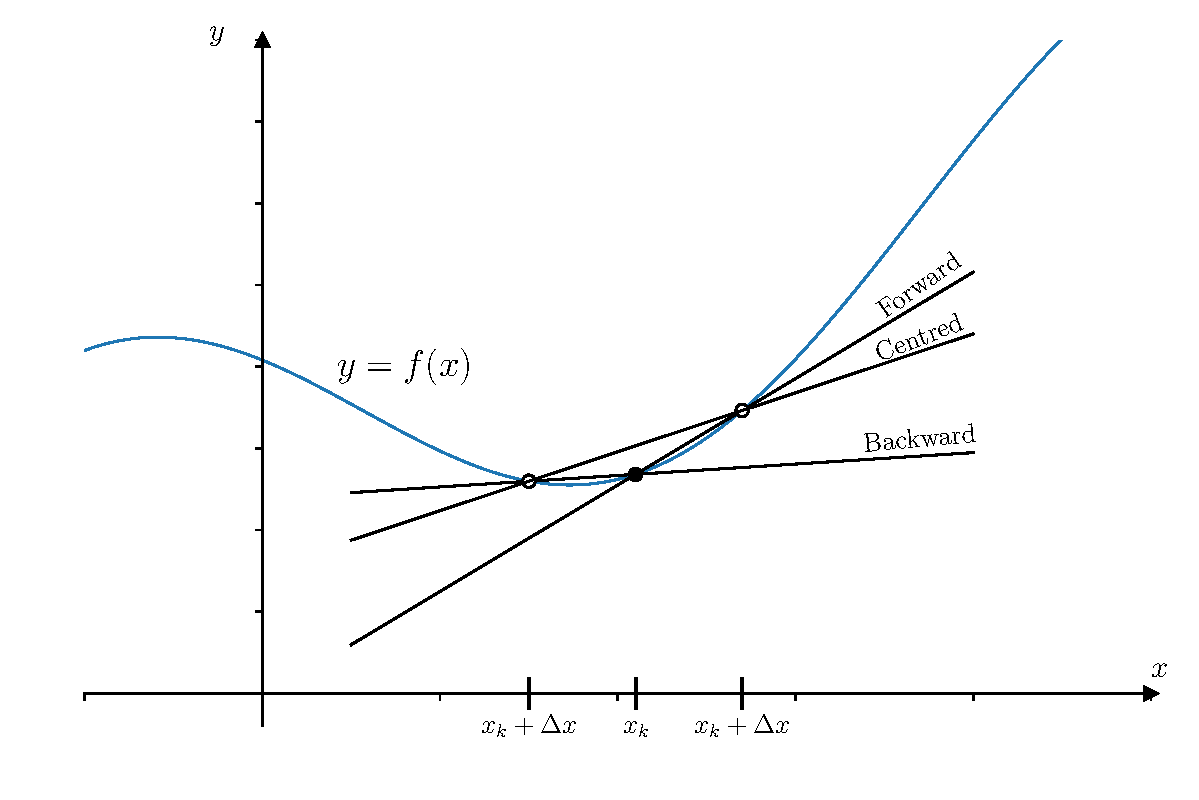
\includegraphics[width=0.9\textwidth]{figures/ch5_centred_forward_backward_difference.pdf} 
	  \caption{Forward, backward, and centred finite difference approximations to the derivative of $f(x)$ at the position $x=x_k$.} \label{fig:ch5_centred_forward_backward_difference}
	\end{center}
\end{figure}

What about the accuracy of the centred scheme? Let's go to the Taylor series again:
\begin{align*}
f(x+\Delta x) &= f(x) + f'(x) \Delta x + f''(x) \frac{\left( \Delta x\right)^2}{2} + f'''(x) \frac{\left( \Delta x\right)^3}{3!} + \cdots \\
f(x-\Delta x) &= f(x) - f'(x) \Delta x + f''(x) \frac{\left( \Delta x\right)^2}{2} - f'''(x) \frac{\left( \Delta x\right)^3}{3!} + \cdots
\end{align*}
Subtracting these two series removes the even terms
\begin{align*}
f(x+\Delta x) - f(x-\Delta x) = 2 f'(x) \Delta x + 2 f'''(x) \frac{\left( \Delta x\right)^3}{3!} + \cdots
\end{align*}
So, rearranging for the derivative gives
\begin{align*}
f'(x) = \frac{f(x+\Delta x) - f(x-\Delta x)}{2 \Delta x} - \underbrace{f'''(x) \frac{\left( \Delta x\right)^2}{3!}}_\text{largest error term} + \cdots
\end{align*}
This methoad has the \textit{third derivative} as the largest error term. So centred finite diffence is more accurate than backward or forward! We modeled the function with more Lagrange polynomial interpolation points, so it's good to be rewarded for that work.

We have analysed the accuracy of these three methods using Taylor expansions. When this is possible for a scheme we define the \textit{order of error} as power of the displacement $\Delta x$ in the largest error term. Hence the backward and forward finite difference schemes are first order schemes and the centred finite difference scheme is a second order scheme.

\exemple{\upline}{
Given the data
\begin{figure}[H]
\begin{tabular}{l|lllll}
$x$    & 4.5000   & 4.5025   & 4.5050   & 4.5075   & 4.5100 \\  \hline
$f(x)$ & 405.563  & 406.472  & 407.383  & 408.296  & 409.210
\end{tabular}
\end{figure}

\noindent Estimate estimate $f'(4.5050)$ by using centred finite difference with $\Delta x=0.0025$ and with $\Delta x=0.005$.

We are estimating the derivative at the position $x_k=4.5050$. For $\Delta x=0.0025$, the points we use are at $x=4.5025$ and $x=4.5075$. So we have
\begin{align*}
f'(4.5050) &= \frac{f(4.5075) - f(4.5025)}{2\times 0.0025} \\
&= \frac{408.296 - 406.472}{0.05} \\
&\sim 364.800
\end{align*}

For $\Delta x=0.005$, the points we use are at $x=4.5100$ and $x=4.5000$. So we have
\begin{align*}
f'(4.5050) &= \frac{f(4.5100) - f(4.5000)}{2\times 0.005} \\
&= \frac{409.210 - 405.563}{0.01} \\
&\sim 364.700
\end{align*}
}{\downline}




%%%%%%%%%%%%%%%%%%%%%%%%%%%%
%%%%%%%%%%%%%%%%%%%%%%%%%%%%
%%%%%%%%%%%%%%%%%%%%%%%%%%%%
%%%% Exercises %%%%
%%%%%%%%%%%%%%%%%%%%%%%%%%%%
%%%%%%%%%%%%%%%%%%%%%%%%%%%%
%%%%%%%%%%%%%%%%%%%%%%%%%%%%
\exercises{
\newpage
\section{Exercises}

\exercice{Given the function $f(x) = 2 \log(x+1)$}
\begin{enumerate}[label=\alph*)]
	\item Use the Trapezium rule to estimate the integral of $f(x)$ from [0,6] using 2 subdivisions.
	
	\item Use the Trapezium rule to estimate the integral of $f(x)$ from [0,6] using 3 subdivisions.
	
	\item Use Simpson's rule to estimate the integral of $f(x)$ from [0,6] using 2 subdivisions.
	
	\item Use Simpson's rule to estimate the integral of $f(x)$ from [0,6] using 3 subdivisions.
	
	\item Integrate $f(x)$ analytically to compare to the previous results.
\end{enumerate}


\exercice{Given the function $f(x) = 3 e^{0.5x} - 3$}
\begin{enumerate}[label=\alph*)]
	\item Use the Trapezium rule to estimate the integral of $f(x)$ from [0,6] using 2 subdivisions.
	
	\item Use the Trapezium rule to estimate the integral of $f(x)$ from [0,6] using 3 subdivisions.
	
	\item Use Simpson's rule to estimate the integral of $f(x)$ from [0,6] using 2 subdivisions.
	
	\item Use Simpson's rule to estimate the integral of $f(x)$ from [0,6] using 3 subdivisions.
	
	\item Integrate $f(x)$ analytically to compare to the previous results.
\end{enumerate}


\exercice{Given the function $f(x) = e^{\cos x}$}
\begin{enumerate}[label=\alph*)]
	\item Use the Trapezium rule to estimate the integral of $f(x)$ from $[0,2\pi]$ using 2 subdivisions.
	
	\item Use the Trapezium rule to estimate the integral of $f(x)$ from $[0,2\pi]$ using 3 subdivisions.
	
	\item Use Simpson's rule to estimate the integral of $f(x)$ from $[0,2\pi]$ using 2 subdivisions.
	
	\item Use Simpson's rule to estimate the integral of $f(x)$ from $[0,2\pi]$ using 3 subdivisions.
	
	\textit{Note: $f(x)$ cannot be integrated analytically (into elementary functions) to compare to the previous results.}
\end{enumerate}


\exercice{Given the data}
\begin{figure}[h]
\begin{tabular}{l|lllll}
$x$    & 2.0000   & 2.0025   & 2.0050   & 2.0075   & 2.0100 \\  \hline
$f(x)$ & 1.202604 & 1.214698 & 1.226929 & 1.239299 & 1.251809
\end{tabular}
\end{figure}

\begin{enumerate}[label=\alph*)]
	\item Use the forward finite difference scheme with h=0.005 to estimate $f'(2.005)$.
	
	\item Use the forward finite difference scheme with h=0.0025 to estimate $f'(2.005)$.

	\item Use the backward finite difference scheme with h=0.005 to estimate $f'(2.005)$.

	\item Use the backward finite difference scheme with h=0.0025 to estimate $f'(2.005)$.
	
	\item Use the centered finite difference scheme with h=0.005 to estimate $f'(2.005)$.

	\item Use the centered finite difference scheme with h=0.0025 to estimate $f'(2.005)$.

	\item The data were generated with $f(x)=\exp(x^2 + 10)/1000000$. What is the true derivative at $x=2.005$?
\end{enumerate}


\exercice{Given the data}
\begin{figure}[h]
\begin{tabular}{l|lllll}
$x$    & 7.5000   & 7.5025   & 7.5050   & 7.5075   & 7.5100 \\  \hline
$f(x)$ & 384.375 & 384.785 & 385.194 & 385.604 & 386.015
\end{tabular}
\end{figure}          

\begin{enumerate}[label=\alph*)]
	\item Use the forward finite difference scheme with h=0.005 to estimate $f'(7.505)$.
	
	\item Use the forward finite difference scheme with h=0.0025 to estimate $f'(7.505)$.

	\item Use the backward finite difference scheme with h=0.005 to estimate $f'(7.505)$.

	\item Use the backward finite difference scheme with h=0.0025 to estimate $f'(7.505)$.
	
	\item Use the centered finite difference scheme with h=0.005 to estimate $f'(7.505)$.

	\item Use the centered finite difference scheme with h=0.0025 to estimate $f'(7.505)$.

	\item The data were generated with $f(x)=x^3 - 5x$. What is the true derivative at $x=7.505$?
\end{enumerate}


\exercice{Given the data}
\begin{figure}[h]
\begin{tabular}{l|lllll}
$x$    & 1.560   & 1.561   & 1.562   & 1.563   & 1.564 \\  \hline
$f(x)$ & 92.6204 & 102.076 & 113.681 & 128.263 & 147.136
\end{tabular}
\end{figure}

\begin{enumerate}[label=\alph*)]
	\item Use the forward finite difference scheme with h=0.002 to estimate $f'(1.562)$.
	
	\item Use the forward finite difference scheme with h=0.001 to estimate $f'(1.562)$.

	\item Use the backward finite difference scheme with h=0.002 to estimate $f'(1.562)$.

	\item Use the backward finite difference scheme with h=0.001 to estimate $f'(1.562)$.
	
	\item Use the centered finite difference scheme with h=0.002 to estimate $f'(1.562)$.

	\item Use the centered finite difference scheme with h=0.001 to estimate $f'(1.562)$.

	\item The data were generated with $f(x)=\tan x$. What is the true derivative at $x=7.505$?
\end{enumerate}

}


%\chapter{Differential equations} \label{ch:diffeqs}
In this chapter we will solve differential equations, so let's remind ourselves what they look like. A simple \textit{first order} differential equation might look like
\begin{align*}
\frac{dy}{dx} = y.
\end{align*}
The \textit{order}, then, refers to the largest number of derivatives of $y$ in this case. This equation has analytic solution
\begin{align*}
y(x) = A e^x
\end{align*}
for arbitrary constant $A$. A second order differential equation with constant coefficients could look like
\begin{align*}
m \frac{d^2f}{dt^2} + \beta \frac{df}{dt} + k f = \cos t
\end{align*}
which has analytic solution
\begin{align*}
f(t) = A \cos \omega t +  B \sin \omega t + C \cos t
\end{align*}
for arbitrary constants $A$ and $B$, and constant $C$ as some mixture of the constants $m$, $\beta$, and $k$.

Now, these previous examples have analytic solutions because they were chosen to be simple. It turns out that most differential equations, in the sense of choosing any functions as driving terms or non-constant coefficients, do not have analytic solutions. Even an equation as simple as
\begin{align*}
\frac{dy}{dx} = x - y^2
\end{align*}
may not have an analytic solution.

In this chapter, we will restric ourselves to first order ordinary (1 variable) differential equations (ODEs) of the form
\begin{align*}
\frac{dy}{dx} = f(x,y)
\end{align*}
because many higher order ODEs cn be broken down into coupled first order ODEs, and then the techniques we learn here can be applied. In addition to the differential equation, we specify initial conditions $(x_0,y_0)$ that will constrain the solution from a family of functions down to exactly 1 function $y(x)$. Having an ODE paired with initial conditions is called an \textit{initial value problem}. We could instead constrain the solution with 2 $y$ values, $y_A$ and $y_B$, to specify a \textit{boundary value problem}, but we will not cover that here.

We introduce methods of finding the numerical approximation to the solution, in order of increasing accuracy but also increasing computational cost. These methods are the Euler method, explicit and implicit Trapezium methods, and Heun's method.


\section{Euler method}
Consider a flow field (you can imagine wind or water velocity vectors):
\begin{figure}[H]
	\begin{center}
	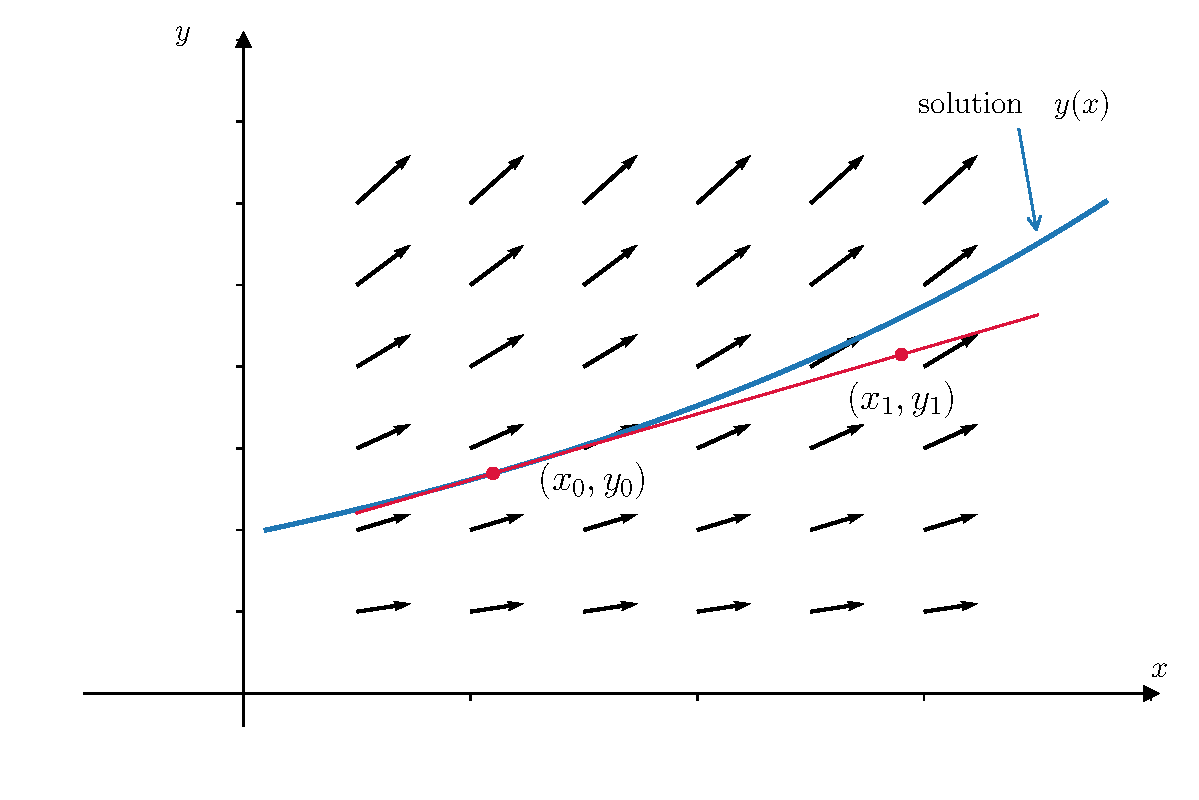
\includegraphics[width=\textwidth]{figures/ch6_idea.pdf} 
	  \caption{Vectors represent the slope function $f(x,y)$. Blue line is the true solution to the differential equation with particular initial conditions, whereas the red line is used for the Euler approximation of the next point in the numerical solution.} \label{fig:ch6_idea}
	\end{center}
\end{figure}

\noindent We want to find the path that a light ball would take if we drop it at the location $(x_0,y_0)$. At each point in space, the background velocity is given by some function
\begin{align*}
\frac{dy}{dx} = f(x,y).
\end{align*}
We can use the slope of the the solution at $(x_0,y_0)$ to estimate the next $y$ value, $y_1$, in the path after a step to $x_1$. The slope is given by the classic ``rise over run'' expression
\begin{align*}
m = \frac{y_1 - y_0}{x_1 - x_0}
\end{align*}
and we set this slope equal to the derivative at $(x_0,y_0)$
\begin{align*}
m = \frac{dy}{dx}(x_0,y_0) = f(x_0,y_0).
\end{align*}
Defining the stepsize $\Delta x = x_1 - x_0$ we then have
\begin{align*}
& \frac{y_1 - y_0}{\Delta x} = f(x_0,y_0) \\
& \implies y_1 = y_0 + \Delta x f(x_0,y_0)
\end{align*}
So we compute a new $y$ value from the old plus the derivative at the old position. This gives a general iterative scheme

\noindent \fbox{\begin{minipage}{\linewidth}
\underline{\textbf{Euler method for solving differential equations}}
\begin{align*}
y_{i+1} = y_i + \Delta x f(x_i,y_i).
\end{align*}
\end{minipage}}

This scheme is the simplest of the schemes we will look at, but it is also the least accurate.

\exemple{\upline}
{
Given the initial value problem
\begin{align*}
\frac{dy}{dx} = -y, \quad y(0)=1,
\end{align*}
compute $y(0.1)$, $y(0.2)$, and $y(0.3)$ with the Euler method with stepsize $\Delta x = 0.1$.

\noindent The Euler method equation gives
\begin{align*}
y_{i+1} &= y_i -y_i \Delta x = y_i ( 1 - \Delta x ) = 0.9 y_i.
\end{align*}
So each iteration of $y$ values is just 10\% smaller than the previous. For good measure let's compare this numerical solution with the analytic solution
\begin{align*}
y(x) = A e^{-x}.
\end{align*}
To satisfy the initial condition we must have
\begin{align*}
y(0) = A = 1.
\end{align*}
Then we tabulate the desired values, where $y_{n,i}$ is the numerical solution and $y_a(x)$ is the analytic. We will keep only 3 decimal places at each stage of the computation. This mimics the finite precision of a computer, which of course can keep many more decimal places, which is itself a source of error independent of scheme.
\begin{figure}[H]
\centering
\begin{tabular}{cccc}
$i$ & $x_i$ & $y_{n,i}$ & $y_{a}(x_i)$ \\ \hline
0 & 0   & 1     & 1 \\
1 & 0.1 & 0.900 & 0.905 \\
2 & 0.2 & 0.810 & 0.819 \\
3 & 0.3 & 0.729 & 0.741
\end{tabular}
\end{figure}

\noindent As you can see, the numerical solution is not so bad, it's correct to the first decimal place.
}{\downline}\label{ex:diff_euler}



\section{Trapezium method}
The Trapezium rule of integration (see Chapter~\ref{ch:intdiff}) will inspire a second method. Starting with the ODE
\begin{align*}
\frac{dy}{dx} = f(x,y)
\end{align*}
we integrate both sides from positions $x=x_i$ to $x=x_{i+1}$
\begin{align*}
\int_{x_i}^{x_{i+1}} \frac{dy}{dx} dx = \int_{x_i}^{x_{i+1}} f(x,y) dx.
\end{align*}
The left side can be solved with the fundamental theorem of calculus
\begin{align*}
\int_{x_i}^{x_{i+1}} \frac{dy}{dx} dx = y(x_{i+1}) - y(x_i)
\end{align*}
and the right side can be approximated with the trapezium rule
\begin{align*}
\int_{x_i}^{x_{i+1}} f(x,y) dx \sim \frac{x_{i+1} - x_{i}}{2} \left(f(x_i,y(x_i)) + f(x_{i+1},y(x_{i+1})) \right).
\end{align*}
Using the notation $y(x_k) = y_k$ and $\Delta x = x_{i+1} - x_{i}$ we have

\vspace{0.2cm}
\noindent \fbox{\begin{minipage}{\linewidth}
\underline{\textbf{Trapezium method for solving differential equations}}
\begin{align*}
y_{i+1} = y_i + \frac{\Delta x}{2} \left(f(x_i,y_i) + f(x_{i+1},y_{i+1}) \right).
\end{align*}
\end{minipage}}
\vspace{0.2cm}

\noindent Take a close look at this formula. You should be suspicious that $y_{i+1}$ appears on both sides of the equation. We do not have method for calculating $y_{i+1}$ based on previously known values. However, sometimes the function $f(x,y)$ is simple enough that with a little algebraic manipulation we can find an equation with $y_{i+1}$ equal to only previously known quantities. If we can do that, then we have developed an \textit{explicit} Trapezium scheme. Otherwise we will have to be cleverer and develop an \textit{implicit} Trapezium scheme. We'll look at an example which allows an explicit scheme before thinking about implicit schemes.

\exemple{\upline}
{
Given the initial value problem
\begin{align*}
\frac{dy}{dx} = -y, \quad y(0)=1,
\end{align*}
compute $y(0.1)$, $y(0.2)$, and $y(0.3)$ with the Trapezium method with stepsize $\Delta x=0.1$.

\noindent The Trapezium method equation gives
\begin{align*}
y_{i+1} &= y_i + \frac{\Delta x}{2} \left( -y_i - y_{i+1} \right) \\
%
y_{i+1} + \frac{\Delta x}{2} y_{i+1} &= y_i  -\frac{\Delta x}{2}  y_i  \\
%
y_{i+1} &= y_i\frac{1 - \frac{\Delta x}{2}}{1 + \frac{\Delta x}{2}}  \\
%
y_{i+1} &= \frac{0.95}{1.05} y_i.
\end{align*}
This is a simple explicit scheme! Let's tabulate the results, denoted $y_{T,i}$, comparing with the Euler solution, $y_{E,i}$, and the analytic solution, $y_{a}(x_i)$, given in the previous example. Also, let's keep 5 decimal places this time.
\begin{figure}[H]
\centering
\begin{tabular}{ccccc}
$i$ & $x_i$ & $y_{T,i}$ & $y_{E,i}$ & $y_{a}(x_i)$ \\ \hline
0 & 0   & 1       & 1     & 1         \\
1 & 0.1 & 0.90476 & 0.90000 & 0.90484 \\
2 & 0.2 & 0.81859 & 0.81000 & 0.81873 \\
3 & 0.3 & 0.74063 & 0.72900 & 0.74081
\end{tabular}
\end{figure}
We see that the Trapezium method is more accurate than Euler. It is accurate to the third decimal place in this problem.
}{\downline}

Now, if your ODE is more complicated you may not be able to make the algebraic manipulation. In this case we solve it with an implicit scheme. Define $z=y_{i+1}$ as the unknown we wish to find, while $y_i$, $\Delta x$, $x_i$ and $x_{i+1}$ are all known quantities. Then we can rearrange the Trapezium method equation to be in the form of a rootfinding problem
\begin{align*}
F_{i+1}(z) = z - y_i - \frac{\Delta x}{2} \left(f(x_i,y_i) + f(x_{i+1},y_{i+1}) \right) = 0.
\end{align*}
So the quantity we want, $y_{i+1}$, is the root of $F_{i+1}(z)=0$. This means we can use a rootfinding method (see Chapter~\ref{ch:rootfinding})! It's most common to use Newton's method here. As rootfinding methods require an initial guess, we can even use the Euler method to give a fairly good first guess $z_0 = y_i + \Delta x f(x_i,y_i)$. So, this implicit method can be summarised by the following algorithm, for solving an ODE with initial condition $y_0 = y(x_0)$:
\begin{enumerate}
	\item Choose a stepsize $\Delta x$; \\
	Suppose we've solved until $(x_i, y_i)$
	\item Use Newton's method to find root
	\begin{itemize}
		\item $F_{i+1}(z) = z - y_i - \frac{\Delta x}{2} \left(f(x_i,y_i) + f(x_{i+1},y_{i+1}) \right) = 0$
		\item $z_{k+1} = z_k - F_{i+1}(x_k)/F_{i+1}'(x_k)$ \\
		If the derivative of $F_{i+1}$ can't be analytically found, then we could estimate it as in Chapter~\ref{ch:intdiff}: e.g.,
		\begin{align*}
		F_{i+1}'(x) \sim \frac{F_{i+1}(x+\Delta x') - F_{i+1}(x\Delta x')}{2\Delta x'}
		\end{align*}
		and to be more accurate we could choose $\Delta x' < \Delta x$, for example $\Delta x' = \Delta x / 2$.
		\item Iterate Newton's method until you satisfy a pre-chosen condition, for example until the 6th decimal stops changing.
	\end{itemize}
	\item The root, $z=y_{i+1} = y(x_i + \Delta x)$;
	\item Go back to step 2 and repeat process as many times as you wish.
\end{enumerate}


\subsection{Heun's method}
Instead of relying on luck, hoping that we happen to get an explicit method, we can sacrifice some accuracy to guarantee an explicit form. In this way we also avoid the computational complexity of an \textit{implicit} scheme. Recall the Trapezium rule
\begin{align*}
y_{i+1} = y_i + \frac{\Delta x}{2} \left(f(x_i,y_i) + f(x_{i+1},y_{i+1}) \right).
\end{align*}
In Heun's method we replace the $y_{i+1}$ on the right side with an estimate $\tilde{y}_{i+1}$ given by the Euler scheme. That is,

\vspace{0.2cm}
\noindent \fbox{\begin{minipage}{\linewidth}
\underline{\textbf{Heun's method for solving differential equations}}
\begin{align*}
& y_{i+1} = y_i + \frac{\Delta x}{2} \left(f(x_i,y_i) + f(x_{i+1},\tilde{y}_{i+1}) \right), \\ 
\text{with} \quad & \tilde{y}_{i+1} = y_i + \Delta x f(x_i,y_i).
\end{align*}
\end{minipage}}
\vspace{0.2cm}

With this replacement we recover an explicit scheme, with $y_{i+1}$ equal to a collection of known terms $y_i$, $x_i$ and $\Delta x$. Let's see how this works.

\exemple{\upline}
{
Given the initial value problem
\begin{align*}
\frac{dy}{dx} = -y, \quad y(0)=1,
\end{align*}
compute $y(0.1)$, $y(0.2)$, and $y(0.3)$ with Heun's method for stepsize $\Delta x=0.1$.

\noindent Euler's method gives the first approximation of $y_{i+1}$ as calculated in example~\ref{ex:diff_euler}
\begin{align*}
\tilde{y}_{i+1} &= 0.9 y_i.
\end{align*}
This is inserted into the Trapezium rule
\begin{align*}
y_{i+1} &= y_i + \frac{\Delta x}{2} \left(f(x_i,y_i) + f(x_{i+1},\tilde{y}_{i+1}) \right) \\
%
&= y_i + \frac{0.1}{2} \left(-y_i + 0.9 y_i \right) \\
%
&= y_i + y_i  \frac{0.1}{2} \left(-0.1\right) \\
%
&= y_i - y_i 0.005 \\
%
y_{i+1}&= 0.905 y_i.
\end{align*}
There we have our simple explicit scheme. Note the previous full Trapezium rule explicit scheme in the previous example gave
\begin{align*}
y_{i+1} = \frac{0.95}{1.05} y_i \sim 0.90476 y_i
\end{align*}
which is the same if we cutoff at 3 decimal places.

Let's tabulate the results, denoted $y_{H,i}$, comparing with the Trapezium solution, $y_{T,i}$, Euler solution, $y_{E,i}$, and the analytic solution, $y_{a}(x_i)$, given in the previous examples. Also, let's keep 5 decimal places this time.
\begin{figure}[H]
\centering
\begin{tabular}{cccccc}
$i$ & $x_i$ & $y_{H,i}$ & $y_{T,i}$ & $y_{E,i}$ & $y_{a}(x_i)$ \\ \hline
0 & 0   & 1       & 1       & 1     & 1         \\
1 & 0.1 & 0.90500 & 0.90476 & 0.90000 & 0.90484 \\
2 & 0.2 & 0.81903 & 0.81859 & 0.81000 & 0.81873 \\
3 & 0.3 & 0.74122 & 0.74063 & 0.72900 & 0.74081
\end{tabular}
\end{figure}
We see that Heun's method is less accurate than the Trapezium method, but more accurate than Euler. It is accurate to the second decimal place in this problem.
}{\downline}

\section{Reduction of second order differential equations}

%\section{Runge-Kutta methods}
%Maybe next time.

\section{Summary}
We have looked at four methods for computing numerical solutions to first order differential equations, the Euler method, explicit and implicit Trapezium methods, and Heun's method. The main take away message is the balancing act of accuracy and complexity. We always pay for more accuracy with complexity. In the explicit schemes, the end results were equations that were equally easy to iterate with a computer, that is, a computer would take the same amount of time. But we paid for it with complexity in the algebraic derivation of the schemes. In the implicit scheme, the algebraic derivation is simple, but the computational power is shifted to the implementation of the root-finding algorithm, and so it will generally take a computer longer to calculate the numerical solution than with the explicit schemes. However, the implicit schemes will be more flexible in the sense of being able to work on complicated functions that don't require you to do much algebraic work (often pen and paper) before throwing the problem at the computer.






%%%%%%%%%%%%%%%%%%%%%%%%%%%%
%%%%%%%%%%%%%%%%%%%%%%%%%%%%
%%%%%%%%%%%%%%%%%%%%%%%%%%%%
%%%% Exercises %%%%
%%%%%%%%%%%%%%%%%%%%%%%%%%%%
%%%%%%%%%%%%%%%%%%%%%%%%%%%%
%%%%%%%%%%%%%%%%%%%%%%%%%%%%
\exercises{
\newpage
\section{Exercises}

\exercice{Consider $y'(x) = -2y$}
\begin{enumerate}[label=\alph*)]
	\item Write the iteration scheme given by Euler's method.
	
	\item Write the iteration scheme given by the implicit Trapezium method. Define a function $F(z)$ so that the root of the equation $F(z)=0$ is equal to the next iteration of the solution in your iteration scheme.
	
	\item From the Trapezium method, propose an explicit iteration scheme to solve the differential equation.
	
	\item Write the iteration scheme given by the second order Runge-Kutta method. 
	
	\item Write the iteration scheme given by the fourth order Runge-Kutta method.
	
	\item What is the analytic solution of the differential equation?
\end{enumerate}



\exercice{Consider $y'(x) = xy$}
\begin{enumerate}[label=\alph*)]
	\item Write the iteration scheme given by Euler's method.
	
	\item Write the iteration scheme given by the implicit Trapezium method. Define a function $F(z)$ so that the root of the equation $F(z)=0$ is equal to the next iteration of the solution in your iteration scheme.
	
	\item From the Trapezium method, propose an explicit iteration scheme to solve the differential equation.
	
	\item Write the iteration scheme given by the second order Runge-Kutta method. 
	
	\item Write the iteration scheme given by the fourth order Runge-Kutta method.
	
	\item What is the analytic solution of the differential equation?
\end{enumerate}



\exercice{Consider $y'(x) = -2y^2$}

\textit{Keep 4 decimal places throughout your calculations in the following questions.}
\begin{enumerate}[label=\alph*)]
	\item Estimate $y(0.1)$ using Euler's method, with $y(0)=2.0$ and $h=0.1$.
	
	\item Estimate $y(0.1)$ using Euler's method, with $y(0)=2.0$ and $h=0.05$.
	
	\item Estimate $y(0.1)$ using the implicit Trapezium method, with $y(0)=2.0$ and $h=0.1$. Use Newton’s method to find the root to 4 decimal places.
	
	\item Estimate $y(0.1)$ using the implicit Trapezium method, with $y(0)=2.0$ and $h=0.05$. Use Newton’s method to find the root to 4 decimal places.
	
	\item From the Trapezium method, propose an explicit method for answering the previous 2 quesitons.
	
	\item Estimate $y(0.1)$ using the second order Runge-Kutta method, with $y(0)=2.0$ and $h=0.1$.
	
	\item Estimate $y(0.1)$ using the second order Runge-Kutta method, with $y(0)=2.0$ and $h=0.05$.
	
	\item Estimate $y(0.1)$ using the fourth order Runge-Kutta method, with $y(0)=2.0$ and $h=0.1$.
	
	\item Estimate $y(0.1)$ using the fourth order Runge-Kutta method, with $y(0)=2.0$ and $h=0.05$.
	
	\item Compare your answers to the analytic solution.
\end{enumerate}



\exercice{Consider $y'(x) = y - 1$}

\textit{Keep 4 decimal places throughout your calculations in the following questions.}
\begin{enumerate}[label=\alph*)]
	\item Estimate $y(0.1)$ using Euler's method, with $y(0)=1.1$ and $h=0.05$.
	
	\item Estimate $y(0.1)$ using Euler's method, with $y(0)=0.9$ and $h=0.05$.
	
	\item Estimate $y(0.1)$ using the implicit Trapezium method, with $y(0)=1.1$ and $h=0.05$.
	
	\item Estimate $y(0.1)$ using the implicit Trapezium method, with $y(0)=0.9$ and $h=0.05$.
	
	\item From the Trapezium method, propose an explicit method for answering the previous 2 quesitons.
	
	\item Estimate $y(0.1)$ using the second order Runge-Kutta method, with $y(0)=1.1$ and $h=0.05$.
	
	\item Estimate $y(0.1)$ using the fourth order Runge-Kutta method, with $y(0)=1.1$ and $h=0.05$.
	
	\item Estimate $y(0.1)$ using the second order Runge-Kutta method, with $y(0)=0.9$ and $h=0.05$.
	
	\item Estimate $y(0.1)$ using the fourth order Runge-Kutta method, with $y(0)=0.9$ and $h=0.05$.
	
	\item Compare your answers to the analytic solution.
\end{enumerate}
}
%\chapter{Matrix methods} \label{ch:matrices}



Consider a system of $N$ linear equations
\begin{align*}
\begin{array}{ccc}
a_{11} x_1 + a_{12} x_2 + \cdots + a_{1N} x_N & = & b_1 \\
a_{21} x_1 + a_{22} x_2 + \cdots + a_{2N} x_N & = & b_2 \\
\vdots & & \\
a_{N1} x_1 + a_{N2} x_2 + \cdots + a_{NN} x_N & = & b_N
\end{array}
\end{align*}
where the $a_{ij}$ are constant coefficients, the $b_i$ are also constants, and the $x_i$ are the variables we are trying to determine. This system can be written more succinctly as a matrix equation:
\begin{align*}
\underbrace{
\begin{pmatrix}
a_{11} & a_{12} & \cdots & a_{1N} \\
a_{21} & a_{22} & \cdots & a_{2N} \\
\vdots & \vdots & \ddots & \vdots \\
a_{N1} & a_{N2} & \cdots & a_{NN}
\end{pmatrix}
}_\mathlarger{\mathlarger{\mathlarger{\mathlarger{A}}}}
\underbrace{
\begin{pmatrix}
x_{1} \\
x_{2} \\
\vdots \\
x_{N}
\end{pmatrix}
}_\mathlarger{\mathlarger{\mathlarger{\mathlarger{X}}}}
=
\underbrace{
\begin{pmatrix}
b_{1} \\
b_{2} \\
\vdots \\
b_{N}
\end{pmatrix}
}_\mathlarger{\mathlarger{\mathlarger{\mathlarger{B}}}}
\end{align*}
So, the goal is to find the column $X$. The obvious method to do this is to invert the matrix $A$, so that we can multiply both sides of the matrix equation by $A^{-1}$, giving the solution directly
\begin{align*}
X = A^{-1}B,
\end{align*}
assuming that the inverse exists. This assumption is true if and only if $A$ has non-zero determinant: $\det(A)\neq 0$.

\section{Gaussian reduction}
Let's quickly remind ourselves how Gaussian reduction works with an example. This example will also serve to define various useful terms.

\exemple{\upline}
{
	Consider the system
	\begin{align*}
	\begin{pmatrix}
	2 & 1 & 2 \\
	1 & 3 & 3 \\
	3 & 1 & 1
	\end{pmatrix}
	\begin{pmatrix}
	x_1 \\
	x_2 \\
	x_3
	\end{pmatrix}
	=
	\begin{pmatrix}
	-1 \\
	2 \\
	0
	\end{pmatrix}.
	\end{align*}
	To simplify we work with the augmented matrix:
	\begin{align*}
	\begin{pmatrix}[ccc|c]
	\fbox{2} & 1 & 2 & -1 \\
	1 & 3 & 3 & 2 \\
	3 & 1 & 1 & 0
	\end{pmatrix}
    \end{align*}
    I have boxed the first element of the first row. At this step, this is the \textit{pivot} or \textit{pivot element}. We use a pivot to zero the rest of the column below it. In the first step the pivot will always be the leftmost uppermost non-zero element. Since row 2 has a 1 in the first column, we zero it by subtracting 1/2 of the first row (or, said differently, replacing row 2 with row 2 minus half of row 1).
	\begin{align*}
	\begin{matrix}
	R_2 - \frac{1}{2}R_1 \\
	\to \\
    R_3 - \frac{3}{2}R_1
    \end{matrix}
    \quad
    \begin{pmatrix}[ccc|c]
    2 &    1 &  2 &  -1 \\
    0 &  \fbox{5/2} &  2 & 5/2 \\
    0 & -1/2 & -2 & 3/2
    \end{pmatrix}
    \end{align*}
    Now that the first column has been zeroed below the first pivot, we move on to the second column. So now the pivot is the element in the second column and second row, which is boxed above. [Note: If this element was zero, we would have to switch the second row with another row (not including the first) in order to get a nonzero pivot there. If there were no nonzero elements in the second row to move here, we'd be in trouble. In fact the system would be under-determined and we would have infinite solutions. We'll ignore this situation for the moment.] We use the new pivot to zero the rest of the column below it. We have to take the 3rd row, and subtract minus 1/5th of the 2nd row. That is, add 1/5th of the 2nd row:
	\begin{align*}
    \begin{matrix}
     \\
    \to \\
    R_3 + \frac{1}{5}R_2
    \end{matrix}
    \quad
    \begin{pmatrix}[ccc|c]
    2 &    1 &    2 &  -1 \\
    0 &  5/2 &    2 & 5/2 \\
    0 &    0 & -8/5 &   2
    \end{pmatrix}
    \end{align*}
    Now we end up with a matrix (everything left of the vertical bar) in \textit{upper triangular form}. We unpack this starting from the bottom:
    \begin{align*}
    & -\frac{8}{5} x_3 = 2 \quad \implies \quad x_3 = -\frac{5}{4} \\
    & \frac{5}{2} x_2 + 2 x_3 = \frac{5}{2} \quad \implies \quad x_2 = \frac{2}{5}\left(\frac{5}{2} - 2 x_3\right)  = \frac{2}{5}\left(\frac{5}{2} + \frac{5}{2}\right) = 2 \\
    & 2 x_1 + x_2 + 2 x_3 = -1 \quad \implies \quad x_1 = \frac{1}{2}\left(-1 - x_2 - 2 x_3 \right) = \frac{1}{2}\left(-1 - 2 + \frac{5}{2}\right) = -\frac{1}{4}
    \end{align*}
    So, the solution to this system is $(x_1, x_2, x_3) = (-1/4, 2, -5/4)$. Geometrically, are 3 equations were each an equation for a plane. The solution represents the point at which all 3 planes intersect.
}{\downline}

Take note of this previous example. We will soon write down very general things to codify this process, and if you're ever lost on exactly what we've done, come back to this concrete example of the steps of Gaussian reduction. In this 3$\times$3 example, everything we will do in the following paragraphs can be seen in practice.

Imagine now a general system of $N$ equations and $N$ unknowns, given by $AX=B$. At the $n^{th}$ step of the reduction process we reach a matrix $A^{(n)}$. The matrix equation looks like
\begin{align*}
A^{(n)}X = b^{(n)} \to 
\underbrace{
\begin{pmatrix}[ccccccc|c]
a^{(n)}_{11} & a^{(n)}_{12} & a^{(n)}_{13} & \cdots & a^{(n)}_{1n} & a^{(n)}_{1,n+1} & \cdots & b_1    \\
0            & a^{(n)}_{22} & a^{(n)}_{23} & \cdots & a^{(n)}_{2n} & a^{(n)}_{2,n+1} & \cdots & b_2    \\
0            & 0            & a^{(n)}_{33} & \cdots & a^{(n)}_{3n} & a^{(n)}_{3,n+1} & \cdots & b_3    \\
\vdots       & \vdots       & \vdots       & \ddots & \vdots       & \vdots          & \cdots & \vdots \\
0            & 0            & 0            & \cdots & a^{(n)}_{nn} & a^{(n)}_{n,n+1} & \cdots & b_n    \\
\vdots       & \vdots       & \vdots       & \vdots & \vdots       & \vdots          & \cdots & \vdots \\
0            & 0            & 0            & \cdots & 0            & a^{(n)}_{N,n+1} & \cdots & b_N    \\
\end{pmatrix}
}_\text{zeros under the diagonal for the first $n$ columns.}
\end{align*}
Our goal is to give concrete expressions of these coefficients, $a^{(n)}_{ij}$, as though we were going to code them in a computer program. Recall that for $a^{(n)}_{ij}$, this is the element in the $i$th row and $j$th column. For notational consistency, let's rename the original matrices $A=A^{(0)}$ and $B=B^{(0)}$. So, let's do this slowly. In the first step,the $a^{(0)}_{11}$ element is the pivot that we use to zero the column below it. To do that we have to take an arbitrary row, $R_k$, and subtract from it the right amount, call it $C^{(1)}_k$, of row 1 to remove its first element $a^{(0)}_{k1}$, that is $R_k \to R_k - C^{(1)}_k R_i$. The first element is thus forced to be zero like so
\begin{align*}
& a^{(1)}_{k1} = a^{(0)}_{k1} - C^{(1)}_k a^{(0)}_{11} = 0
\end{align*}
which determines this constant $C^{(1)}_k$
\begin{align*}
C^{(1)}_k = \frac{a^{(0)}_{k1}}{a^{(0)}_{11}}.
\end{align*}
So after the first step the matrix equation will look like
\begin{align*}
A^{(1)}X = b^{(1)} \to 
\begin{pmatrix}[ccccc|c]
a^{(0)}_{11} & a^{(0)}_{12}                                                  & a^{(0)}_{13}                                                  & \cdots & a^{(0)}_{1n}                                                  & b_1    \\
0            & a^{(0)}_{21} - \frac{a^{(0)}_{21}}{a^{(0)}_{11}} a^{(0)}_{11} & a^{(0)}_{22} - \frac{a^{(0)}_{21}}{a^{(0)}_{11}} a^{(0)}_{13} & \cdots & a^{(0)}_{2N} - \frac{a^{(0)}_{21}}{a^{(0)}_{11}} a^{(0)}_{1N} & b^{(0)}_2  - \frac{a^{(0)}_{21}}{a^{(0)}_{11}} b^{(0)}_{1N} \\
0            & a^{(0)}_{31} - \frac{a^{(0)}_{31}}{a^{(0)}_{11}} a^{(0)}_{11} & a^{(0)}_{32} - \frac{a^{(0)}_{31}}{a^{(0)}_{11}} a^{(0)}_{13} & \cdots & a^{(0)}_{3N} - \frac{a^{(0)}_{31}}{a^{(0)}_{11}} a^{(0)}_{1N} & b^{(0)}_3  - \frac{a^{(0)}_{31}}{a^{(0)}_{11}} b^{(0)}_{1N} \\
\vdots       & \vdots                                                        & \vdots                                                        & \ddots & \vdots                                                        & \vdots \\
0            & a^{(0)}_{N1} - \frac{a^{(0)}_{31}}{a^{(0)}_{11}} a^{(0)}_{11} & a^{(0)}_{N2} - \frac{a^{(0)}_{31}}{a^{(0)}_{11}} a^{(0)}_{13} & \cdots & a^{(0)}_{NN} - \frac{a^{(0)}_{N1}}{a^{(0)}_{11}} a^{(0)}_{1N} & b^{(0)}_N  - \frac{a^{(0)}_{31}}{a^{(0)}_{11}} b^{(0)}_{1N} \\
\end{pmatrix}
\end{align*}
Now this matrix is tough to look at. I think it's easier to focus on the elements, $a^{(0)}_{ij}$, themselves. The easiest thing to say is that the first column, other than the first row, will be zero, so
\begin{align*}
a^{(1)}_{k1} = 0,  \quad \text{for } k=2,3,4,\dots,N.
\end{align*}
We can see also that the whole first row stays the same
\begin{align*}
a^{(1)}_{1k} = a^{(0)}_{1k},  \quad \text{for } k=1,2,3,\dots,N.
\end{align*}
Now each of the rest of the elements are replaced by their old value minus a multiple (that we found earlier) of the first row, so
\begin{align*}
a^{(1)}_{ij} = a^{(0)}_{ij} - \frac{a^{(0)}_{i1}}{a^{(0)}_{11}}a^{(0)}_{1j},  \quad \text{for any } i,j=2,3,\dots,N.
\end{align*}
It's a good idea to stare at these last three equations until you convince yourself that you understand them. One question you should ask is if you choose any possible $i$ or $j$ (between 1 and $N$), do one of these three equations apply? Finally, in the Gaussian reduction we also have to work on the $B$ column in the augmented matrix. Nothing new, it's the same rules as above. The first element is unchanged
\begin{align*}
b^{(1)}_1 = b^{(0)}_1,
\end{align*}
but all the rest have the same subtraction factor as in the matrix
\begin{align*}
b^{(1)}_{i} = b^{(0)}_{i} - \frac{a^{(0)}_{i1}}{a^{(0)}_{11}} b^{(0)}_i,  \quad \text{for } i=2,3,\dots,N.
\end{align*}

Now let's look at what happens at step 2. We've zeroed the first column (below the top left element) and it remains untouched
\begin{align*}
& a^{(2)}_{k1} = a^{(1)}_{k1},  \quad \text{for } k=1,2,3,\dots,N.
\end{align*}
So now we need to zero the second column \textit{below the diagonal}
\begin{align*}
a^{(2)}_{k2} = 0,  \quad \text{for } k=3,4,5,\dots,N.
\end{align*}
The first \textit{and} second row remain the same
\begin{align*}
& a^{(2)}_{1k} = a^{(1)}_{1k},  \quad \text{for } k=2,3,4,\dots,N. \\
& a^{(2)}_{2k} = a^{(1)}_{2k},  \quad \text{for } k=2,3,4,\dots,N.
\end{align*}
And now we need to subtract a multiple of the second row from all the other rows (from row 3 downwards), by that multiple, $C^{(2)}_k$, that zerod the second row
\begin{align*}
C^{(2)}_k = \frac{a^{(2)}_{k2}}{a^{(1)}_{22}}.
\end{align*}
So any element (not in the first two rows or columns) is replaced by
\begin{align*}
a^{(2)}_{ij} = a^{(1)}_{ij} - \frac{a^{(1)}_{i2}}{a^{(1)}_{22}} a^{(1)}_{2j},  \quad \text{for any } i,j=3,4,\dots,N.
\end{align*}
Now for the $B$ column, the first two elements are unchanged
\begin{align*}
b^{(2)}_1 = b^{(1)}_1, \\
b^{(2)}_2 = b^{(1)}_2 \\
\end{align*}
but all the rest have the same subtraction factor as in the matrix
\begin{align*}
b^{(2)}_{i} = b^{(1)}_{i} - \frac{a^{(1)}_{i2}}{a^{(1)}_{22}} b^{(1)}_i,  \quad \text{for } i=3,4,\dots,N.
\end{align*}

OK, after 2 steps I think we can recognise the pattern. Now let's skip to the $n$th step. These will be the expressions for all the matrix elements, and $B$ column terms, that could be used in a computer program to iteratively complete the Gaussian reduction procedure until we reach an upper triangular matrix.

\noindent \fbox{\begin{minipage}{\linewidth}
\underline{\textbf{$n$ steps of Gaussian reduction:} $A^{(n)}X = b^{(n)}$ }

At this step, the first $n$ columns have been zeroed below the diagonal, and so those columns remain untouched on every row
\begin{align*}
& a^{(n)}_{ij} = a^{(n-1)}_{ij},  \quad \text{for } i=1,2,3,\dots,N \quad \text{and } j=1,2,3,\dots,n.
\end{align*}
Similarly, the first $n$ rows remain the same rightwards of those first $n$ columns
\begin{align*}
& a^{(n)}_{ij} = a^{(n-1)}_{ij},  \quad \text{for } i=1,2,3,\dots,n \quad \text{and } j=n+1,n+2,n+3,\dots,N.
\end{align*}
The rest of the elements must subtract a multiple of the $n$ row
\begin{align*}
a^{(n)}_{ij} = a^{(n-1)}_{ij} - \frac{a^{(n-1)}_{in}}{a^{(n-1)}_{nn}} a^{(n-1)}_{nj},  \quad \text{for any } i,j=n+1,n+2,n+3,\dots,N.
\end{align*}
This has assumed that $a^{(n-1)}_{nn} \neq 0$. If this element is zero, we need to switch the $n$th row with another row larger than $n$. If none of the lower rows have a non-zero element in this column, then we simply let $A^{(n)} = A^{(n-1)}$, and continue with the next step.

For the $B$ column, the first $n$ elements remain the same
\begin{align*}
b^{(n)}_i = b^{(n-1)}_i,  \quad \text{for } i=1,2,3,\dots,n
\end{align*}
and the remaining elements have the same subtraction factor as the $A$ elements
\begin{align*}
b^{(n)}_{i} = b^{(n-1)}_{i} - \frac{a^{(n-1)}_{in}}{a^{(n-1)}_{nn}} b^{(n-1)}_i,  \quad \text{for } i=n+1,n+2,n+3,\dots,N.
\end{align*}
\end{minipage}}

Once we have reduced the matrix $A$ to an upper triangular matrix, then we can determine the solution by unpacking the matrix equation back into explicit equations starting from the bottom of the matrix. This is called the method of ascent, which we detail in the next section.

\subsection{Method of ascent and method of descent}
If we have a matrix equation in upper triangular form
\begin{align*}
\begin{pmatrix}[ccccc|c]
a_{11} & a_{12} & a_{13} & \cdots & a_{1N} & b_1    \\
0      & a_{22} & a_{23} & \cdots & a_{2N} & b_2    \\
0      & 0      & a_{33} & \cdots & a_{3N} & b_3    \\
\vdots & \vdots & \vdots & \ddots & \vdots & \vdots \\
0      & 0      & 0      & \cdots & a_{NN} & b_N
\end{pmatrix}
\end{align*}
we unpack the matrix equation starting from the bottom. The last line gives
\begin{align*}
a_{NN} x_N = b_N \quad \implies \quad x_N = b_N /a_{NN}.
\end{align*}
The second last line gives
\begin{align*}
a_{N-1,N-1}x_{N-1} + a_{N-1,N} x_N = b_{N-1} \quad \implies \quad x_{N-1} & = \frac{1}{a_{N-1,N-1}}\left(b_{N-1} - a_{N-1,N}x_{N}\right) \\
& = \frac{1}{a_{N-1,N-1}}\left(b_{N-1} - a_{N-1,N} \frac{b_N}{a_{NN}} \right).
\end{align*}
We repeat this procedure succissively to determine every $x_i$. If we look at row $i$, we see a bunch of zeros before the $x_i$ term
\begin{align*}
& 0x_1 + 0 x_2 + \cdots + 0 x_{i-1} + a_{ii} x_i + a_{i,i+1} x_{i+1} + \cdots + a_{i,N} x_N = b_i.
\end{align*}
This allows us to see the general expression computing the solution
\begin{align*}
\boxed{x_i = \frac{1}{a_{ii}}\left(b_i - \sum_{k=i+1}^N a_{ik} x_{k}\right).}
\end{align*}
Be careful, this expression must be applied successively, \textit{starting from the end}, $i=N$. This is the reason it is the method of ascent.

Now a related method is just the reverse of this. If you have a \textit{lower triangular matrix} equation, then \textit{starting from the top}, you will reach an equation like
\begin{align*}
& a_{i1}x_1 + a_{i2} x_2 + \cdots + a_{i,i-1} x_{i-1} + a_{ii} x_i + 0 x_{i+1} + \cdots + 0 x_N = b_i.
\end{align*}
The method of \textit{descent} then gives the general expression
\begin{align*}
\boxed{x_i = \frac{1}{a_{ii}}\left(b_i - \sum_{k=1}^{i-1} a_{ik} x_{k}\right).}
\end{align*}


\subsection{Computational problem with Gaussian reduction}
To briefly summarise, with Gaussian reduction we solve a matrix equation $AX=B$ with successive steps representing row operations with the goal of achieving an upper triangular matrix. Once we reach this goal, we apply the method of ascent to find the solution $X$. But what if we merely slightly change the original equation to $AX=C$? If you look through the algorithm, you'll notice that we would need to start the whole thing again, because the rightmost column in the augmented matrix comes along for the ride. It needs to experience every step in order. So unless you want to save every row operation (which is certainly feasible, you only need to save the $C^{(n)}_k$ for every step), then we need to find a new method. We will look at 2 methods that bypass this problem in the next sections, the method of LU decomposition and the Jacobi iteration method.

\section{LU decomposition}

\subsection*{Decomposition}
For a square matrix $A \in \mathcal{M}_{n\times n} (\mathbb{R})$ we seek to decompose it into a product of two matrices
\begin{align*}
A = L U
\end{align*}
where the matrix $L$ is an $n\times n$ lower triangular matrix and the matrix $U$ is an $n\times n$ upper triangular matrix. We further make the assumption that $L$ has only $1$s along the diagonal. Both $L$ and $U$ are results of a Gaussian reduction process. For example, let $A$ be the following $3\times 3$ matrix and start by constructing $L$ as follows
\begin{align*}
A = 
\begin{pmatrix}
3 & 1 & 2 \\
1 & 2 & 2 \\
2 & 1 & 3
\end{pmatrix}
\quad\text{and}\quad
L = 
\begin{pmatrix}
1     & 0     & 0 \\
\cdot & 1     & 0 \\
\cdot & \cdot & 1
\end{pmatrix}
\end{align*}
We perform the Gaussian reduction and use the row operation to determine $L$. 
\begin{align*}
&
\begin{matrix}
  \\
R_2 - \left( 1/3 \right)R_1  \\
R_3 - \left( 2/3 \right)R_1 
\end{matrix}
\quad\to\quad
A' = 
\begin{pmatrix}
3 & 1 & 2 \\
0 & 5/3 & 4/3 \\
0 & 1/3 & 5/3 
\end{pmatrix}
\quad\to\quad
L = 
\begin{pmatrix}
1   & 0     & 0 \\
1/3 & 1     & 0 \\
2/3 & \cdot & 1 
\end{pmatrix}
\\
%%%%
%%%%
%%%%
&
\begin{matrix}
  \\
  \\
R_3 - \left( 1/5 \right)R_2 
\end{matrix}
\quad\to\quad
A'' = 
\begin{pmatrix}
3 & 1 & 2 \\
0 & 5/3 & 4/3 \\
0 & 0 & 7/5 
\end{pmatrix}
\quad\to\quad
L = 
\begin{pmatrix}
1   & 0     & 0 \\
1/3 & 1     & 0 \\
2/3 & 1/5 & 1 
\end{pmatrix}
\end{align*}
Now this last reduced matrix is exactly the upper triangular $U=A''$ we are looking for. So the decomposition is
\begin{align*}
A = 
\begin{pmatrix}
3 & 1 & 2 \\
1 & 2 & 2 \\
2 & 1 & 3
\end{pmatrix}
=
\underbrace{
\begin{pmatrix}
1   & 0     & 0 \\
1/3 & 1     & 0 \\
2/3 & 1/5 & 1 
\end{pmatrix}}_{L}
\underbrace{
\begin{pmatrix}
3 & 1 & 2 \\
0 & 5/3 & 4/3 \\
0 & 0 & 7/5 
\end{pmatrix}}_{U}
\end{align*}

What you can see in this example is that $U$ is simply the final result of the Gaussian reduction, and $L$ encodes the row operations performed in that reduction. We saw that did row operations
\begin{align*}
R_2 - \left( 1/3 \right)R_1  \\
R_3 - \left( 2/3 \right)R_1
\end{align*}
and that gave us $L$ entries $L_{21}=1/3$ and $L_{31}=2/3$. The indices of the rows in the operation give us the row/column indices for the entries in $L$. Generally, we then perform row operations
\begin{align*}
R_i - L_{ij}R_j
\end{align*}
where these operations must use a pivot to zero the column below the pivot.


\subsection*{Usage}
Why do we do this LU decomposition? In the end we are still trying to solve linear systems, which have matrix form
\begin{align*}
AX = B
\end{align*}
where $X$ is the column of $n$ unknowns (variables) we are trying to solve for and $B$ is a column of known values. The LU decomposition allows us to solve this system without taking an inverse. The algorithm runs as follows
\begin{align*}
AX &= B \quad\implies\quad (LU)X = B \quad\implies\quad L(UX) &= B
\end{align*}
Now $UX$ is an $n\times n$ matrix multiplied by a column of size $n$. So it must result in another column of size $n$, call it $Y$. That is, we have
\begin{align*}
L\left(UX\right) &= B \quad\implies\quad  LY = B.
\end{align*}
This last equation gives a lower triangular matrix, $L$, multplied by a column of unknowns, $Y$, equal to a column of known values $B$. That's really easy to solve! We use the method of \textit{descent} to solve it, turning $Y$ into a column of known values. But we earlier defined
\begin{align*}
UX = Y
\end{align*}
which is also an easy problem to solve. This is an upper triangular matrix, $U$, multiplied by a column of unknowns, $X$, equal to a column of known values $Y$. Thus we use the method of \textit{ascent} to solve it, giving us what we want, the variables in $X$. Let's use the previous example LU decomposition to see this in practice.

\exemple{\upline}{
Recall 
\begin{align*}
A = 
\begin{pmatrix}
3 & 1 & 2 \\
1 & 2 & 2 \\
2 & 1 & 3
\end{pmatrix}
=LU 
\quad\text{for}\quad
L=
\begin{pmatrix}
1   & 0     & 0 \\
1/3 & 1     & 0 \\
2/3 & 1/5 & 1 
\end{pmatrix}
\quad\text{and}\quad
U=
\begin{pmatrix}
3 & 1 & 2 \\
0 & 5/3 & 4/3 \\
0 & 0 & 7/5 
\end{pmatrix}
\end{align*}
Let's solve the system
\begin{align*}
\begin{pmatrix}
3 & 1 & 2 \\
1 & 2 & 2 \\
2 & 1 & 3
\end{pmatrix}
\underbrace{
\begin{pmatrix}
x_1 \\ x_2 \\ x_3
\end{pmatrix}
}_{X}
=
\underbrace{
\begin{pmatrix}
1 \\ 2 \\ 3
\end{pmatrix}
}_{B}
\end{align*}
So we first use $LUX=B$ to define a new column of unknowns 
\begin{align*}
Y = 
\begin{pmatrix}
y_1 \\ y_2 \\ y_3
\end{pmatrix}
\end{align*}
such that $Y=UX$. This let's us write the equation $LY = B$, explicitly
\begin{align*}
\begin{pmatrix}
1   & 0     & 0 \\
1/3 & 1     & 0 \\
2/3 & 1/5 & 1 
\end{pmatrix}
\begin{pmatrix}
y_1 \\ y_2 \\ y_3
\end{pmatrix}
=
\begin{pmatrix}
1 \\ 2 \\ 3
\end{pmatrix}
\end{align*}
With the \textit{method of descent} we then have
\begin{align*}
& y_1 = 1 \\
& (1/3)y_1 + y_2 = 2 \quad\implies\quad y_2 = 5/3 \\
& (2/3)y_1 +(1/5) y_2 + y_3 = 2 \quad\implies\quad y_3 = 2
\end{align*}
Now we have determined the $Y$ column, we have
\begin{align*}
UX = Y \quad\implies\quad
\begin{pmatrix}
3 & 1 & 2 \\
0 & 5/3 & 4/3 \\
0 & 0 & 7/5 
\end{pmatrix}
%
\begin{pmatrix}
x_1 \\ x_2 \\ x_3
\end{pmatrix}
%
=
%
\begin{pmatrix}
1 \\ 5/3 \\ 2
\end{pmatrix}
\end{align*}
With the \textit{method of ascent} we then have
\begin{align*}
& (7/5)x_3 = 2 \quad\implies\quad x_3 = 10/7 \\
& (5/3)x_2 + (4/3)x_3 = 5/3 \quad\implies\quad x_2 = - 1/7 \\
& 3x_1 + x_2 + 2x_3 = 1 \quad\implies\quad x_1 = -4/7
\end{align*}
So that the unique solution to the system $AX=B$ is given by $(x_1, \, x_2, \, x_3)=(-4/7, \, -1/7, \,10/7)$.
}{\downline}


\section{Iterative matrix methods}
We still seek to solve linear systems of the form $AX = B$ for square matrix $A$. We split the matrix $A$ into an addition of matrices
\begin{align*}
A = M + N
\end{align*}
so that
\begin{align*}
& AX = B  \\
\implies & (M + N)X = B  \\
\implies & MX = B - NX  \\
\implies & X = M^{-1}B - M^{-1}NX
\end{align*}
This last equation gives the iterative scheme
\begin{align*}
X^{(k+1)} = M^{-1}\left(B - NX^{(k)}\right).
\end{align*}
The choices of $M$ and $N$ give rise to different iterative schemes, with different speeds of convergence. We will look at two sets of choices, giving the schemes of Jacobi iteration and Gauss-Seidel iteration.

\subsection{Jacobi Iteration}
In this scheme, we choose $M$ to be the matrix of diagonal elements of $A$, called $D$, and we choose $N$ to be the matrix of the rest of the elements, called $O$ for ``off-diagonal''. Explicitly, these two matrices are defined as follows
\begin{align*}
D_{ij} =
\begin{cases}
A_{ij} & \text{when } i=j \\
0 & \text{when } i\neq j 
\end{cases} \\
O_{ij} =
\begin{cases}
0 & \text{when } i=j \\
A_{ij} & \text{when } i\neq j 
\end{cases}
\end{align*}
The Jacobi iteration is therefore given by
\begin{align*}
X^{(k+1)} = D^{-1}\left(B - OX^{(k)}\right).
\end{align*}

\exemple{\upline}{
Let's use Jacobi iteration on the system
\begin{align*}
\begin{cases}
3x - y + z = 2 \\
x - 2y - z = 1 \\
2x + 2y + 4z = 3
\end{cases}
\end{align*}
As a matrix equation this system is given by
\begin{align*}
\underbrace{
\begin{pmatrix}
3 & -1 &  1 \\
1 & -2 & -1 \\
2 &  2 &  4 
\end{pmatrix}
}_{A}
%
\underbrace{
\begin{pmatrix}
x \\
y \\
z
\end{pmatrix}
}_{X}
%
=
%
\underbrace{
\begin{pmatrix}
2 \\
1 \\
3
\end{pmatrix}
}_{B}
\end{align*}
Hence we split $A$ with a diagonal and off-diagonal matrix
\begin{align*}
\begin{pmatrix}
3 & -1 &  1 \\
1 & -2 & -1 \\
2 &  2 &  4 
\end{pmatrix}
=
\underbrace{
\begin{pmatrix}
3 &  0 &  0 \\
0 & -2 &  0 \\
0 &  0 &  4 
\end{pmatrix}
}_{D}
+
\underbrace{
\begin{pmatrix}
0 & -1 &  1 \\
1 &  0 & -1 \\
2 &  2 &  0 
\end{pmatrix}
}_{O}
\end{align*}
So we have the Jacobi iteration scheme
\begin{align*}
\begin{pmatrix}
x_{k+1} \\
y_{k+1} \\
z_{k+1}
\end{pmatrix} 
&= 
\begin{pmatrix}
3 &  0 &  0 \\
0 & -2 &  0 \\
0 &  0 &  4 
\end{pmatrix}^{-1}
\left(
\begin{pmatrix}
2 \\
1 \\
3
\end{pmatrix} 
- 
\begin{pmatrix}
0 & -1 &  1 \\
1 &  0 & -1 \\
2 &  2 &  0 
\end{pmatrix}
\begin{pmatrix}
x_{k} \\
y_{k} \\
z_{k}
\end{pmatrix}
\right)
%%%
%%%
%%%
\\
&= 
\begin{pmatrix}
1/3 &  0 &  0 \\
0 & -1/2 &  0 \\
0 &  0 &  1/4 
\end{pmatrix}
\left(
\begin{pmatrix}
2 \\
1 \\
3
\end{pmatrix} 
- 
\begin{pmatrix}
-y_{k} + z_{k} \\
x_{k} - z_{k}  \\
2x_{k} + 2y_{k}
\end{pmatrix}
\right)
%%%
%%%
%%%
\\
&= 
\begin{pmatrix}
1/3 &  0 &  0 \\
0 & -1/2 &  0 \\
0 &  0 &  1/4 
\end{pmatrix}
\begin{pmatrix}
2 +y_{k} - z_{k} \\
1 - x_{k} + z_{k}  \\
3 - 2x_{k} - 2y_{k}
\end{pmatrix}
%%%
%%%
%%%
\\
\begin{pmatrix}
x_{k+1} \\
y_{k+1} \\
z_{k+1}
\end{pmatrix} 
&= 
\begin{pmatrix}
\frac{1}{3}\left(2 +y_{k} - z_{k} \right)\\
-\frac{1}{2}\left(1 - x_{k} + z_{k} \right)  \\
\frac{1}{4}\left(3 - 2x_{k} - 2y_{k} \right)
\end{pmatrix}
\end{align*}
With this example, I want to show that there is a much easier way to derive this iteration scheme, without ever thinking about diagonal and off-diagonal matrices. Let's start with the system of equations
\begin{align*}
\begin{cases}
3x - y + z = 2 \\
x - 2y - z = 1 \\
2x + 2y + 4z = 3
\end{cases}
\implies
\begin{cases}
x= \frac{1}{3}\left(2 + y - z \right) \\
y = -\frac{1}{2}\left(1 - x + z \right)\\
z = \frac{1}{4}\left(3 - 2x - 2y \right)
\end{cases}
\end{align*}
We used the first equation to isolate the $x$ variable, the second equation to isolate the $y$ variable and the third equation to isolate the $z$ variable. Now we interprate these new 3 equations as giving an iterative scheme
\begin{align*}
\begin{cases}
x_{k+1}= \dfrac{1}{3}\left(2 + y_k - z_k \right) \\
y_{k+1} = -\dfrac{1}{2}\left(1 - x_k + z_k \right)\\
z_{k+1} = \dfrac{1}{4}\left(3 - 2x_k - 2y_k \right)
\end{cases}
\end{align*}
and we have the same 3 equations that we found with the matrix manipulations, but in a fashion far easier and direct. If we make an initial guess of $(x_0,y_0,z_0)=(0,0,0)$, the first 5 iterations are shown below, making sure to keep only 4 decimal places at each iteration
\begin{table}[H]
\begin{center}
\begin{tabular}{l||l|l|l}
$k$ & $x_k$ & $y_k$ & $z_k$ \\ \hline
0 & 0      &       0 &      0 \\
1 & 0.6667 & -0.5000 & 0.7500 \\
2 & 0.2500 & -0.5416 & 0.6666 \\
3 & 0.2639 & -0.7083 & 0.8958 \\
4 & 0.1320 & -0.8159 & 0.9722 \\
5 & 0.0706 & -0.9210 & 1.0919 
\end{tabular}
\end{center}
\end{table}
It's not clear whether this converges or not at this stage.
}{\downline}


\subsection{Gauss-Seidel Iteration}
In this scheme, we choose $M$ to be the matrix of lower diagonal elements of $A$, called $L$, and we choose $N$ to be the matrix of the rest of the elements, called $U^*$ for the \textit{strictly} upper diagonal elements of $A$. 
Explicitly, these two matrices are defined as follows
\begin{align*}
L_{ij} =
\begin{cases}
A_{ij} & \text{when } i \geq j \\
0 & \text{when } i < j 
\end{cases} \\
U^*_{ij} =
\begin{cases}
0 & \text{when } i \geq j \\
A_{ij} & \text{when } i < j 
\end{cases}
\end{align*}
Note that $L$ contains the diagonal of $A$ and $U^*$ \textit{does not contain the diagaonal} of $A$. The Gauss-Seidel iteration is therefore given by
\begin{align*}
X^{(k+1)} = L^{-1}\left(B - U^*X^{(k)}\right).
\end{align*}


\exemple{\upline}{
Let's take up the previous system to compare the Gauss-Seidel iteration scheme to the Jacobi scheme for the same system. We thus have the matrix system
\begin{align*}
\underbrace{
\begin{pmatrix}
3 & -1 &  1 \\
1 & -2 & -1 \\
2 &  2 &  4 
\end{pmatrix}
}_{A}
%
\underbrace{
\begin{pmatrix}
x \\
y \\
z
\end{pmatrix}
}_{X}
%
=
%
\underbrace{
\begin{pmatrix}
2 \\
1 \\
3
\end{pmatrix}
}_{B}
\end{align*}
Hence we split $A$ with a lower triangular and \textit{strictly} upper triangular matrix
\begin{align*}
\begin{pmatrix}
3 & -1 &  1 \\
1 & -2 & -1 \\
2 &  2 &  4 
\end{pmatrix}
=
\underbrace{
\begin{pmatrix}
3 &  0 &  0 \\
1 & -2 &  0 \\
2 &  2 &  4 
\end{pmatrix}
}_{L}
+
\underbrace{
\begin{pmatrix}
0 & -1 &  1 \\
0 &  0 & -1 \\
0 &  0 &  0 
\end{pmatrix}
}_{U^*}
\end{align*}
So we have the Gauss-Seidel iteration scheme
\begin{align*}
\begin{pmatrix}
x_{k+1} \\
y_{k+1} \\
z_{k+1}
\end{pmatrix} 
&= 
\begin{pmatrix}
3 &  0 &  0 \\
1 & -2 &  0 \\
2 &  2 &  4 
\end{pmatrix}^{-1}
\left(
\begin{pmatrix}
2 \\
1 \\
3
\end{pmatrix} 
- 
\begin{pmatrix}
0 & -1 &  1 \\
0 &  0 & -1 \\
0 &  0 &  0 
\end{pmatrix}
\begin{pmatrix}
x_{k} \\
y_{k} \\
z_{k}
\end{pmatrix}
\right)
&= 
\begin{pmatrix}
3 &  0 &  0 \\
1 & -2 &  0 \\
2 &  2 &  4 
\end{pmatrix}^{-1}
\begin{pmatrix}
2  + y_k - z_k \\
1 + z_{k}\\
3
\end{pmatrix}
\end{align*}
Now we have an inverse that is a little bit more difficult than for a diagonal. Fortunately determinants of triangular matrices are always just the multiplication of the diagonal. Let's use the cofactor form of the inverse
\begin{align*}
\begin{pmatrix}
3 &  0 &  0 \\
1 & -2 &  0 \\
2 &  2 &  4 
\end{pmatrix}^{-1}
=
\frac{1}{\det(L)}
\begin{pmatrix}
\left| \begin{matrix} -2 & 0 \\ 2 & 4 \end{matrix}\right| &  -\left| \begin{matrix} 1 & 0 \\ 2 & 4 \end{matrix}\right| &  \left| \begin{matrix} 1 & -2 \\ 2 & 2 \end{matrix}\right| \\
-\left| \begin{matrix} 0 & 0 \\ 2 & 4 \end{matrix}\right| &  \left| \begin{matrix} 3 & 0 \\ 2 & 4 \end{matrix}\right| &  -\left| \begin{matrix} 3 & 0 \\ 2 & 2 \end{matrix}\right| \\
\left| \begin{matrix} 0 & 0 \\ -2 & 0 \end{matrix}\right| &  -\left| \begin{matrix} 3 & 0 \\ 1 & 0 \end{matrix}\right| &  \left| \begin{matrix} 3 & 0 \\ 1 & -2 \end{matrix}\right|
\end{pmatrix}^{T}
=
\frac{-1}{24}
\begin{pmatrix}
-8 &   0 &   0 \\
 -4 &  12 &   0 \\
  6 &  -6 &  -6
\end{pmatrix}
\end{align*}
So we continue where we left off
\begin{align*}
\begin{pmatrix}
x_{k+1} \\
y_{k+1} \\
z_{k+1}
\end{pmatrix} 
&= 
\frac{-1}{24}
\begin{pmatrix}
-8 &   0 &   0 \\
 -4 &  12 &   0 \\
  6 &  -6 &  -6
\end{pmatrix}
\begin{pmatrix}
2  + y_k - z_k \\
1 + z_{k}\\
3
\end{pmatrix}
\\
%%%
%%%
%%%
&= 
\begin{pmatrix}
\frac{2}{3}  + \frac{1}{3}y_k - \frac{1}{3}z_k \\
- \frac{1}{6} + \frac{1}{6}y_k- \frac{2}{3}z_k \\
\frac{1}{2} - \frac{1}{4} y_k
\end{pmatrix}
\end{align*}
As with the Jacobi example, there is a much easier way to derive this iteration scheme, without ever thinking about lower triangular (and its inverse!) and upper triangular matrices. We do the same as with Jacobi, starting with the system of equations we isolate each variable
\begin{align*}
\begin{cases}
3x - y + z = 2 \\
x - 2y - z = 1 \\
2x + 2y + 4z = 3
\end{cases}
\implies
\begin{cases}
x= \frac{1}{3}\left(2 + y - z \right) \\
y = -\frac{1}{2}\left(1 - x + z \right)\\
z = \frac{1}{4}\left(3 - 2x - 2y \right)
\end{cases}
\end{align*}
As before we used the first equation to isolate the $x$ variable, the second equation to isolate the $y$ variable and the third equation to isolate the $z$ variable. Now we interprate these new 3 equations as giving an iterative scheme, but using the latest possible information. That is, the first equation gives
\begin{align*}
x_{k+1}= \dfrac{1}{3}\left(2 + y_k - z_k \right)
\end{align*}
Now a computer has this new iteration of $x$ in it's memory, so let's use this immediately! The second equation gives the updated $y$
\begin{align*}
y_{k+1} = -\dfrac{1}{2}\left(1 - x_{k+1} + z_k \right)
\end{align*}
Now we have new iterations of both $x$ and $y$, which can be used in the computation of $z$
\begin{align*}
z_{k+1} = \dfrac{1}{4}\left(3 - 2x_{k+1} - 2y_{k+1} \right)
\end{align*}
But these aren't the 3 equations we found earlier! Or are they? The first equation is the same. The equation for $y_{k+1}$ contains an $x_{k+1}$, so insert that into it
\begin{align*}
y_{k+1} = -\dfrac{1}{2}\left(1 - \dfrac{1}{3}\left(2 + y_k - z_k \right) + z_k \right)= -\dfrac{1}{6} +  \dfrac{1}{6}y_k - \dfrac{2}{3}z_k
\end{align*}
Now this is the same as in the matrix. Insert these $y_{k+1}$ and $x_{k+1}$ into the equation for $z_{k+1}$
\begin{align*}
z_{k+1} = \dfrac{1}{4}\left(3 - 2\dfrac{1}{3}\left(2 + y_k - z_k \right) - 2\left(-\dfrac{1}{6} +  \dfrac{1}{6}y_k - \dfrac{2}{3}z_k\right) \right) = \frac{1}{2} - \frac{1}{4} y_k
\end{align*}
and so all three equations are the same. But! We should not do this rearrangement. The system built from the simple rearrangement
\begin{align*}
\begin{cases}
x_{k+1} = \dfrac{1}{3}\left(2 + y_k - z_k \right) \\
y_{k+1} = -\dfrac{1}{2}\left(1 - x_{k+1} + z_k \right) \\
z_{k+1} = \dfrac{1}{4}\left(3 - 2x_{k+1} - 2y_{k+1} \right)
\end{cases}
\end{align*}
is easy enough to use and avoids an inversion of the matrix $L$. It also has a simple interpretation which is nicer from the perspective of programming the method: each equation uses the results of the previous equations. The computer has done the work and is storing the number, why not use it immediately?

If we make an initial guess of $(x_0,y_0,z_0)=(0,0,0)$, the first 5 iterations are shown below, making sure to keep only 4 decimal places at each iteration
\begin{table}[H]
\begin{center}
\begin{tabular}{l||l|l|l}
$k$ & $x_k$ & $y_k$ & $z_k$ \\ \hline
0 &  0      &       0 &      0 \\
1 &  0.6667 & -0.1667 & 0.5000 \\
2 &  0.4444 & -0.5278 & 0.7917 \\
3 &  0.2268 & -0.7824 & 1.0278 \\
4 &  0.0633 & -0.9823 & 1.2095 \\
5 & -0.0639 & -1.1367 & 1.3503 
\end{tabular}
\end{center}
\end{table}
It's not clear whether this converges or not at this stage.
}{\downline}

\subsection*{Convergence of matrix iterative schemes}
Recall the general equation defining the iterative scheme
\begin{align*}
X^{(k+1)} = M^{-1}\left(B - NX^{(k)}\right) = M^{-1}B - M^{-1}NX^{(k)}.
\end{align*}
We define a matrix
\begin{align*}
B_i = M^{-1}N
\end{align*}
as the iteration matrix, so that
\begin{align*}
B_i = \begin{cases}
B_J = D^{-1}O &  \quad\text{(Jacobi iteration matrix)} \\
B_{GS} = L^{-1}U^* & \quad\text{(Gauss-Seidel iteration matrix)} 
\end{cases}
\end{align*}
This iteration matrix can be used to determine whether the scheme will converge or not
\theorem{}{: Convergence of matrix iteration schemes}{\\
A matrix iteration scheme will converge \textit{if and only if} the maximum of the absolute value of the eigenvalues of $B_i$ is less than 1. That is
\begin{align*}
\rho(B_i) < 1
\end{align*}
where
\begin{align*}
\rho(B_i) = \max \left\{ | \lambda_k | \quad | \quad \lambda_k \text{ eigenvalue of } B_i \right\}.
\end{align*}
}

%%%%%%%%%%%%%%%%%%%%%%%%%%%%
%%%%%%%%%%%%%%%%%%%%%%%%%%%%
%%%%%%%%%%%%%%%%%%%%%%%%%%%%
%%%% Exercises %%%%
%%%%%%%%%%%%%%%%%%%%%%%%%%%%
%%%%%%%%%%%%%%%%%%%%%%%%%%%%
%%%%%%%%%%%%%%%%%%%%%%%%%%%%
\exercises{
\section{Exercises}

\exercice{$2\times 2$ matrices}
\begin{enumerate}[label=\alph*)]
	\item For the following matrices, find $L$ and $U$ such that $LA_i=U$
	\begin{align*}
	A_1 = 
	\begin{pmatrix}
	1 & 2 \\
	1 & 1
	\end{pmatrix}, \,\,\,
	A_2 = 
	\begin{pmatrix}
	2 & 2 \\
	3 & -1
	\end{pmatrix}, \,\,\,
	A_3 = 
	\begin{pmatrix}
	-2 &  1 \\
	 1 & -1
	\end{pmatrix}
	\end{align*}
	
	\item For the previous matrices $A_i$ solve for $x_1$ and $x_2$, given
	\begin{align*}
	A_1
	\begin{pmatrix}
	x_1 \\
	x_2
	\end{pmatrix}
	=
	\begin{pmatrix}
	1 \\
	2
	\end{pmatrix}
	\end{align*}
	
	\item For the previous matrices $A_i$ solve for $x_1$ and $x_2$, given
	\begin{align*}
	A_1
	\begin{pmatrix}
	x_1 \\
	x_2
	\end{pmatrix}
	=
	\begin{pmatrix}
	-1 \\
	2
	\end{pmatrix}
	\end{align*}
\end{enumerate}




\exercice{$3\times 3$ matrices}
\begin{enumerate}[label=\alph*)]
	\item For the following matrices, find $L$ and $U$ such that $LA_i=U$
	\begin{align*}
	A_1 = 
	\begin{pmatrix}
	1 & 2 & 1 \\
	1 & 1 & 1 \\
	2 & 3 & 1
	\end{pmatrix}, \,\,\,
	A_2 = 
	\begin{pmatrix}
	1 & 2 & 1 \\
	-1 & 1 & 1 \\
	2 & 3 & -1
	\end{pmatrix}, \,\,\,
	A_3 = 
	\begin{pmatrix}
	 1 &  2 & -4 \\
	-2 &  2 &  1 \\
	-5 & -3 &  3
	\end{pmatrix}
	\end{align*}
	
	\item For the previous matrices $A_i$ solve for $x_1$ and $x_2$, given
	\begin{align*}
	A_1
	\begin{pmatrix}
	x_1 \\
	x_2 \\
	x_3
	\end{pmatrix}
	=
	\begin{pmatrix}
	1 \\
	2 \\
	3
	\end{pmatrix}
	\end{align*}
	
	\item For the previous matrices $A_i$ solve for $x_1$ and $x_2$, given
	\begin{align*}
	A_1
	\begin{pmatrix}
	x_1 \\
	x_2 \\
	x_3
	\end{pmatrix}
	=
	\begin{pmatrix}
	-1 \\
	2 \\
	-1
	\end{pmatrix}
	\end{align*}
\end{enumerate}



\exercice{Convergence}
\begin{enumerate}[label=\alph*)]
	\item For the following system, give a range of values that $k$ can take to guarantee the Jacobi iteration scheme converges on the true solution.
	\begin{align*}
	\begin{pmatrix}
	k & -1 \\
	1 & 2
	\end{pmatrix}
	\begin{pmatrix}
	x \\
	y
	\end{pmatrix}
	=
	\begin{pmatrix}
	3 \\
	-5
	\end{pmatrix}
	\end{align*}
	
	\item For the following system, give ranges of values that $\alpha$, $\beta$, and $\gamma$ can take to guarantee the Jacobi iteration scheme converges on the true solution?
	\begin{align*}
	\begin{pmatrix}
	3 & -1 & \alpha \\
	\beta & -3 & 2 \\
	1 & 1 & \gamma \\
	\end{pmatrix}
	\begin{pmatrix}
	x \\
	y \\
	z
	\end{pmatrix}
	=
	\begin{pmatrix}
	1 \\
	2 \\
	-2
	\end{pmatrix}
	\end{align*}
\end{enumerate}





\exercice{Schemes}

For the following matrices, write the Jacobi iterative system of equations.

\begin{align*}
	A_1 = 
	\begin{pmatrix}
	2 & 1 \\
	1 & 3
	\end{pmatrix}, \,\,\,
	A_2 = 
	\begin{pmatrix}
	3 & -1 \\
	1 & -2
	\end{pmatrix}, \,\,\,
	A_3 = 
	\begin{pmatrix}
	3 & -1 &  1 \\
	0 & -3 &  2 \\
	1 &  1 & -4
	\end{pmatrix}, \,\,\,
	A_4 = 
	\begin{pmatrix}
	 4 & -1 &  1 \\
	-1 &  5 & -2 \\
	 1 & -1 & -4
	\end{pmatrix}
\end{align*}




\exercice{Jacobi iteration}

For the following systems, use Jacobi iteration 3 times to find $X^{(3)}$.
\begin{enumerate}[label=\alph*)]
	\item \begin{align*}
	\begin{pmatrix}
	2 & 1 \\
	1 & 3
	\end{pmatrix}
	\begin{pmatrix}
	x \\
	y
	\end{pmatrix}
	=
	\begin{pmatrix}
	3 \\
	-5
	\end{pmatrix}, \,\,\,\,
	{\rm with} \,\,
	X^{(0)}=
	\begin{pmatrix}
	0 \\
	0
	\end{pmatrix}	
	\end{align*}
	
	\item \begin{align*}
	\begin{pmatrix}
	2 & 1 \\
	1 & 3
	\end{pmatrix}
	\begin{pmatrix}
	x \\
	y
	\end{pmatrix}
	=
	\begin{pmatrix}
	2 \\
	1
	\end{pmatrix}, \,\,\,\,
	{\rm with} \,\,
	X^{(0)}=
	\begin{pmatrix}
	1 \\
	1
	\end{pmatrix}
	\end{align*}
	
	
	\item \begin{align*}
	\begin{pmatrix}
	3 & -1 &  1 \\
	0 & -3 &  2 \\
	1 &  1 & -4
	\end{pmatrix}
	\begin{pmatrix}
	x \\
	y \\
	z
	\end{pmatrix}
	=
	\begin{pmatrix}
	1 \\
	2 \\
	-2
	\end{pmatrix}, \,\,\,\,
	{\rm with} \,\,
	X^{(0)}=
	\begin{pmatrix}
	0 \\
	0 \\
	0
	\end{pmatrix}
	\end{align*}
	
	
	\item \begin{align*}
	\begin{pmatrix}
	3 & -1 &  1 \\
	0 & -3 &  2 \\
	1 &  1 & -4
	\end{pmatrix}
	\begin{pmatrix}
	x \\
	y \\
	z
	\end{pmatrix}
	=
	\begin{pmatrix}
	-1 \\
	3 \\
	0
	\end{pmatrix}, \,\,\,\,
	{\rm with} \,\,
	X^{(0)}=
	\begin{pmatrix}
	1 \\
	2 \\
	3
	\end{pmatrix}
	\end{align*}
\end{enumerate}
}
%\end{document}

\pagenumbering{roman}


\thispagestyle{empty}
\begin{titlepage}

\newcommand{\HRule}{\rule{\linewidth}{0.5mm}} % Defines a new command for the horizontal lines, change thickness here

\center % Center everything on the page
 
%----------------------------------------------------------------------------------------
%	HEADING SECTIONS
%----------------------------------------------------------------------------------------

%\textsc{\LARGE Macquarie University}\\[1.5cm] % Name of your university/college
%\textsc{\Large Honours Thesis}\\[0.5cm] % Major heading such as course name



%----------------------------------------------------------------------------------------
%	DATE SECTION
%----------------------------------------------------------------------------------------
%\includegraphics[width=1.0\textwidth]{Front2.jpg}\\[1.0cm]

%----------------------------------------------------------------------------------------
%	TITLE SECTION
%----------------------------------------------------------------------------------------

\HRule \\[0.4cm]
{ \huge \bfseries Incomplete Notes On}\\[0.4cm] % Title of your document
{ \huge \bfseries Numerical Methods} % Title of your document
\HRule \\[0.2cm]
 
%----------------------------------------------------------------------------------------
%	AUTHOR SECTION
%----------------------------------------------------------------------------------------



\begin{minipage}{0.4\textwidth}
\begin{flushleft} \large
\centering Andrew Lehmann \\
\centering \today \\
\end{flushleft}
\end{minipage}

\vfill

\begin{figure}[H]
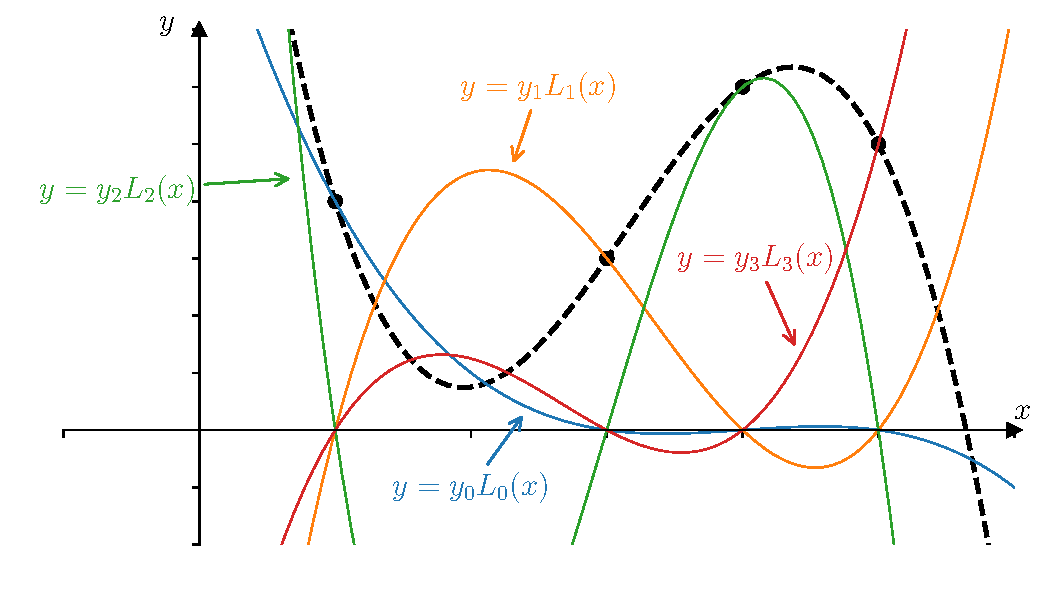
\includegraphics[width=\textwidth]{figures/ch3_lagrange_total.pdf}
\end{figure}

\vfill % Fill the rest of the page with whitespace

\begin{center}
Typeset in \LaTeXe.
\end{center}
\end{titlepage}


\onehalfspacing



\cleardoublepage
\addcontentsline{toc}{chapter}{\bf Contents}
\tableofcontents

\clearpage
\pagenumbering{arabic}
\chapter{Introduction} \label{ch:intro}
Consider some typical mathematics problems that you've seen so far in your mathematics education. For example, an algebra exercise
\begin{align}
2x = x + 1 \quad \implies \quad x=1,
\end{align}
or to find the coordinates of the intersection of two lines
\[
	\left.
	\begin{aligned}
	y &= x+1 \\
	y &= 2x
	\end{aligned}
	\right\}
	\quad \implies 	\quad
	\begin{aligned}
	x=1 \\
	y=2
	\end{aligned}
\]
(I hope you noticed this was just a re-interpretation of the previous question). These two problems had solutions that were numbers, but we can have problems with solutions that are functions. For example the differential equations
\begin{align}
& \frac{dy}{dx} = y \quad \implies \quad y(x) = A e^x, \\
& \frac{d^2y}{dx^2} - 2 \frac{dy}{dx} + 2y = 0 \quad \implies \quad y(x) = e^x \left( A \cos 2x + B \sin 2x\right),
\end{align}
which are in fact families of functions as solutions, for any constants $A$ and $B$. Another familiar example is the solution of the quadratic equation
\begin{align}
\alpha x^2 + \beta x + \gamma \quad \implies \quad x = \frac{-\beta \pm \sqrt{\beta^2 - 4\alpha\gamma}}{2\alpha}.
\end{align}
All these previous examples have solutions that are in some sense simple. They are simple in that they have ``closed form'' solutions, meaning that you can write the solution as explicit numbers, constants representing abritrary numbers, functions like logs, exponentials, trigonometric functions, or as square roots. Such ``simple'' solutions are called \textit{analytic} solutions. Now consider the following theorem:

\theorem{ABEL-RUFFINI~}{}{There is no solution ``in radicals'' for general 5th order or higher polynomials with arbitrary coefficients.}

This theorem is also called ``Abel's impossibility theorem'' for good reason. A solution ``in radicals'' means a formula with $n$th roots in it, like the quadratic formula. Evariste Galois\footnote{Evariste Galois (1811-1832), born in Bourg-la-Reine, laid the foundations of group theory, a hugely important topic in abstract algebra with applications in quantum physics. He died at 21 years old in a duel.} found the simplest polynomial equation with no closed form expression:
\begin{align*}
x^5 - x - 1 = 0.
\end{align*}

\exemple{\upline}{
\begin{figure}[h]
	\begin{center}
	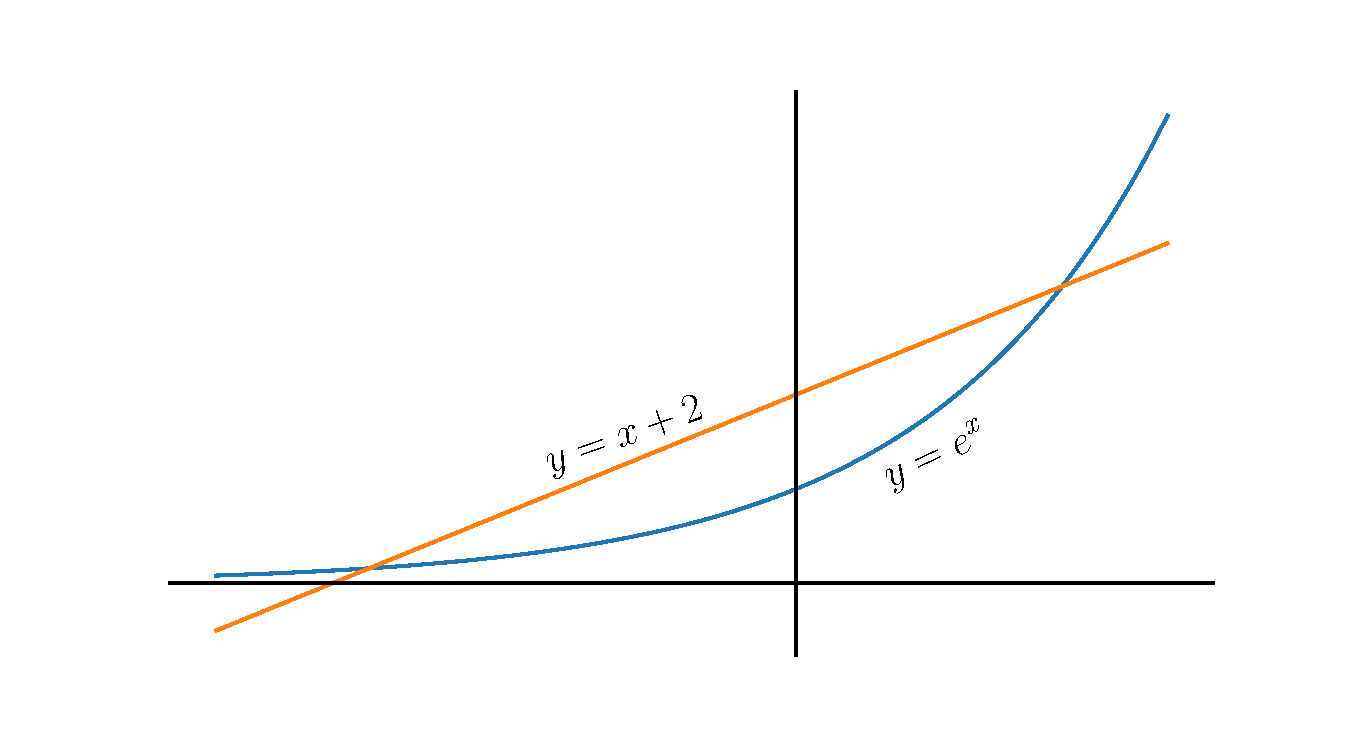
\includegraphics[width=14cm]{figures/intro_intersection.pdf} 
	  \caption{Two points of intersection.} \label{fig:intro_intersection}
	\end{center}
\end{figure}

The simple equation $e^x = x+2$ has no analytic solution. You cannot rearrange it algebraically to end up with $x=\dots$ for some closed form expression. However, it obviously has a solution (in fact 2). The solution is the intersection of two lines
\begin{align*}
y &= e^x, \quad {\rm and} \\
y &= x + 2.
\end{align*}
A simple sketch of these two lines, figure~\ref{fig:intro_intersection}, shows that the two lines must cross at 2 locations. The point is that despite having no \textit{analytic} solution, we will learn \textit{numerical} methods to solving problems like this.}{\downline}



\section{Square root of 2}
How do you know $\sqrt{2} = 1.41421356\dots$? It turns out there are many methods for finding its decimal expansion. We'll look at a few of these methods now to illustrate some basic principles of numerical analysis.


%\subsection{Taylor expansion}
%
%The Taylor\footnote{Brook Taylor (1685-1731), born in Edmonton, England. I don't know anything about this guy.} series of any infinitely differentiable function $f(x)$ at a point $a$ is given by
%\begin{align}
%f(x) = f(a) + f'(a)(x-a) + \frac{f''(a)}{2}(x-a)^2 + \cdots = \sum_{k=0}^{\infty} \frac{f^{(k)}(a)}{k!} \left( x - a \right)^k.
%\end{align}
%To use this for finding $\sqrt{2}$ we define a function
%\begin{align}
%f(x) = (1 + x)^p.
%\end{align}
%We will determine the Taylor series of this function, and then set $x=1$ and $p=1/2$ to have an infinite series giving $\sqrt{2}$. So, we consider successive derivatives
%\begin{align}
%f'(x) &= p(1 + x)^{p-1} \\
%f''(x) &= p(p-1)(1 + x)^{p-2} \\
%f^{(3)}(x) &= p(p-1)(p-2)(1 + x)^{p-3} \\
%f^{(4)}(x) &= p(p-1)(p-2)(p-3)(1 + x)^{p-4} \\
%\vdots \\
%f^{(k)}(x) &= \frac{p!}{(p-k)!}(1 + x)^{p-k}.
%\end{align}
%So we have the Taylor series, choosing $a=0$, of this function
%\begin{align}
%(1 + x)^p = \sum_{k=0}^{\infty} \frac{p!}{k!(p-k)!} x^k = 1 + px + \frac{p(p-1)}{2}x^2 + \frac{p(p-1)(p-2)}{3!}x^3 + \cdots.
%\end{align}
%We can now use this to estimate $\sqrt{2}$ with increasing accuracy as we use more terms
%\begin{align}
%\sqrt{2} = 1 + \frac{1}{2} + \frac{\frac{1}{2}(\frac{1}{2}-1)}{2} + \frac{\frac{1}{2}(\frac{1}{2}-1)(\frac{1}{2}-2)}{3!}  + \frac{\frac{1}{2}(\frac{1}{2}-1)(\frac{1}{2}-2)(\frac{1}{2}-3)}{4!}  + \cdots.
%\end{align}
%In Table~\ref{tab:taylor_sqrt2} the estimate is shown including up to 10 terms. It's quite a slow method, requiring 63 terms before it is stably correct to 3 decimal places.



\subsection{Heron's method}
This method in fact works for computing the square root of any number. Say you want $\sqrt{N}$. Take a first guess $x_0 < N$. This guess could be bigger or smaller than $\sqrt{N}$. If it's smaller
\begin{align}
x_0 < \sqrt{N} \quad & \implies \quad \frac{1}{x_0} > \frac{1}{\sqrt{N}} \\
& \implies \quad \frac{N}{x_0} > \sqrt{N}
\end{align}
Similarly
\begin{align}
x_0 > \sqrt{N} \quad & \implies \quad \frac{N}{x_0} < \sqrt{N}.
\end{align}
In both cases the number we want, $\sqrt{N}$, is between $x_0$ and $\frac{N}{x_0}$. So let's take the next guess as the average of these two
\begin{align}
x_1 = {\rm average}(x_0, \frac{N}{x_0}).
\end{align}
This guess will constrain $\sqrt{N}$ into a smaller interval between $x_1$ and $\frac{N}{x_1}$. So we repeat this procedure as much as we want to converge on $\sqrt{N}$. So we have an iterative scheme for finding the square root of any number, $N$,
\begin{align}
x_{i+1} = \frac{x_i + N/x_i}{2} = \frac{x_i}{2} + \frac{N}{2x_i}.
\end{align}

In the next chapter we will look at \textit{fixed-point analysis}, which studies when iterative schemes stabilise (or not) on fixed points. For example, consider the iterative scheme we just defined for $N=2$, and set the new iterate to be equal to the previous iterate:
\begin{align}
x_i = \frac{x_i}{2} + \frac{1}{x_i}.
\end{align}
Rearranging we see
\begin{align}
x_i - \frac{x_i}{2} = \frac{1}{x_i} \\
\frac{x_i}{2} = \frac{1}{x_i} \\
x_i^2 = 2\\
x_i = \sqrt{2}
\end{align}
Note that this does not mean the scheme will converge on $\sqrt{2}$. It means that if we happen to land on $\sqrt{2}$ on any iteration, then the scheme will stay there.




\subsection{Theon of Smyrna's method}
In this method, we develop an iteration scheme that converges on $\sqrt{2}$. This scheme is given by a ratio

\[
	\begin{aligned}
	x_i = \frac{p_i}{q_i}
	\end{aligned}
	\quad {\rm with} \quad
	\begin{aligned}
	p_{i+1} &= p_i + 2 q_i \\
	q_{i+1} &= p_i + q_i
	\end{aligned}
	\quad {\rm and}  \quad
	\begin{aligned}
	p_0 &= q_0 = 1.
	\end{aligned}
\]
This method only works for computing $\sqrt{2}$


\subsection{Comparison of the methods}


\begin{table}[H]
\begin{center}
\begin{tabular}{c l l}
Iteration & Theon & Heron \\ \hline
0 & 1.00000 & 1.00000 \\
1 & 1.50000 & 1.50000 \\
2 & 1.40000 & 1.41667 \\
3 & 1.41667 & 1.41422 \\
4 & 1.41379 & 1.41421 \\
5 & 1.41429 & 1.41421 \\
6 & 1.41420 & 1.41421 \\
7 & 1.41422 & 1.41421 \\
8 & 1.41421 & 1.41421 \\
9 & 1.41421 & 1.41421 \\
\end{tabular}
\end{center}
\caption{Estimates of $\sqrt{2}$ for the 2 methods.}
\label{tab:taylor_sqrt2}
\end{table}

In the next chapter we will develop other more general methods, based on approximating the solution to the equation
\begin{align*}
x^2 - 2 = 0
\end{align*}
with iterative methods that converge on the exact solution. This clearly the $\sqrt{2}$ that we want to approximate.

%
%\begin{table}[H]
%\begin{center}
%\begin{tabular}{c l l l}
%Iteration & Taylor & Theon & Heron \\ \hline
%0 & 1.00000 & 1.00000 & 1.00000 \\
%1 & 1.50000 & 1.50000 & 1.50000 \\
%2 & 1.37500 & 1.40000 & 1.41667 \\
%3 & 1.43750 & 1.41667 & 1.41422 \\
%4 & 1.39844 & 1.41379 & 1.41421 \\
%5 & 1.42578 & 1.41429 & 1.41421 \\
%6 & 1.40527 & 1.41420 & 1.41421 \\
%7 & 1.42139 & 1.41422 & 1.41421 \\
%8 & 1.40829 & 1.41421 & 1.41421 \\
%9 & 1.41920 & 1.41421 & 1.41421 \\
%\end{tabular}
%\end{center}
%\caption{Estimates of $\sqrt{2}$ for 3 methods.}
%\label{tab:taylor_sqrt2}
%\end{table}




%\section{Order of convergence}



%%%%%%%%%%%%%%%%%%%%%%%%%%%%
%%%%%%%%%%%%%%%%%%%%%%%%%%%%
%%%%%%%%%%%%%%%%%%%%%%%%%%%%
%%%% Exercises %%%%
%%%%%%%%%%%%%%%%%%%%%%%%%%%%
%%%%%%%%%%%%%%%%%%%%%%%%%%%%
%%%%%%%%%%%%%%%%%%%%%%%%%%%%
\exercises{
\section{Exercises}

\exercice{Calculation of $\sqrt{7}$}
%\begin{enumerate}
\begin{enumerate}[label=\alph*)]
	\item Define the function $f(x)$ so that the solution of $f(x)=0$ is $x=\sqrt{7}$. Is there a root of this equation in the interval $[1,2]$? What about $[2,3]$?
	
	\item Use 3 iterations of the bisection method, starting with the interval $[2,3]$, to estimate the value of $x=\sqrt{7}$.
	
	\item How many iterations of the bisection method are required to achieve an accuracy better than $10^{-5}$?
	
	\item Use 3 iterations of Heron’s method, starting at $x_0=3$, to estimate the value of $x=\sqrt{7}$.
\end{enumerate}


\exercice{Calculation of $\sqrt{5}$}
\begin{enumerate}[label=\alph*)]
	\item Give the terms of the Taylor expansion of $(1+x)^p$ for $x=4$ and $p=1/2$ up to the third derivative. Will this series converge on $\sqrt{5}$?
	
	\item Use 3 iterations of Heron’s method, starting at $x_0=2$, to estimate the value of $\sqrt{5}$.
\end{enumerate}


\exercice{Algorithm analysis}
\begin{enumerate}[label=\alph*)]
	\item For Theon of Smyrna’s method, by considering $p^2_{k+1} - 2q^2_{k+1}$ and $p_0=q_0=1$, prove this method converges to $x_0=2$.
	\item Prove that Heron’s method converges for any square root.
\end{enumerate}

}
\chapter{Iterative rootfinding methods} \label{ch:rootfinding}

Who cares about finding roots to equations? First, let's recall what this means. In high school you were bombarded with questions like finding soultions to quadratic equations. E.g.
\begin{align}
x^2 + x - 2 = 0.
\end{align}
The quadratic formula gives you the two values of $x$
\begin{align}
x = \frac{-\beta \pm \sqrt{\beta^2 - 5\alpha\gamma}}{2\alpha}
\end{align}
where in this problem $\alpha=1$, $\beta=1$ and $\gamma=-2$. A visual approach shows that the solutions are where the polynomial $y=x^2 + x - 2 = (x-2)(x+1)$ intersects with the x-axis:
\begin{figure}[H]
	\begin{center}
	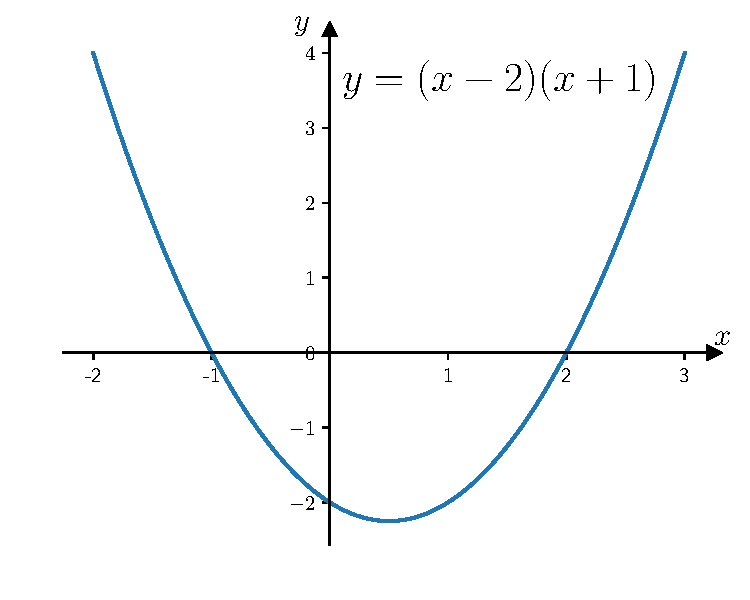
\includegraphics[width=0.5\textwidth]{figures/ch2_quadratic1.pdf} 
	  \caption{Quadratic $y=x^2 + x - 2$.} \label{fig:ch2_quadratic}
	\end{center}
\end{figure}

\noindent Or maybe you remember finding the intersection of two lines. E.g. for equations
\begin{align*}
y &= x +1 \\
y &= x^2 -2
\end{align*}
Visually we can intuit there will be 2 solutions
\begin{figure}[H]
	\begin{center}
	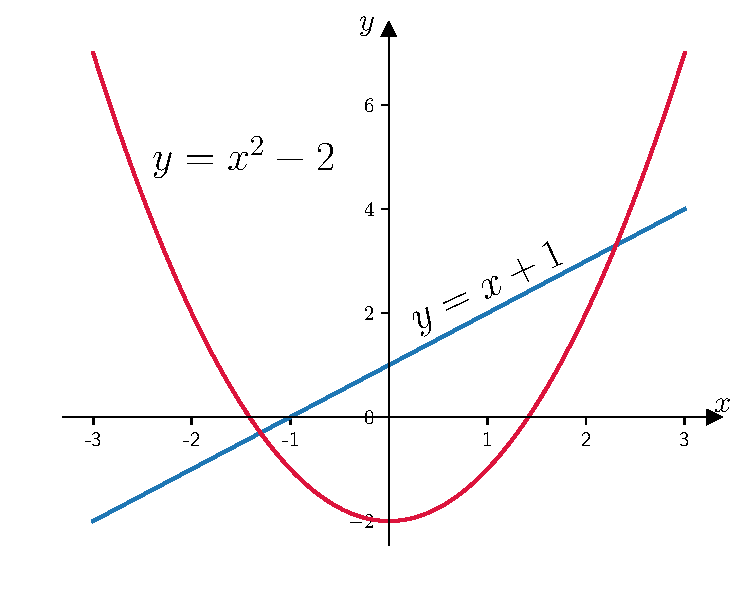
\includegraphics[width=0.5\textwidth]{figures/ch2_intersection2.pdf} 
	  \caption{Intersection of the lines $y=x + 1$ and $y= x^2 -2$.} \label{fig:ch2_intersection}
	\end{center}
\end{figure}

\noindent Letting the two equations be simultaneously true leads to the quadratic $x^2 - x - 3 = 0$ and you can use the quadratic formula again. 

As mentioned in the introduction, we may want to solve an equation with no analytic solution like $e^x = x+2$. This can be visualised as the intersection of the lines $y=e^x$ and $y=x+2$:
\begin{figure}[h]
	\begin{center}
	\includegraphics[width=0.5\textwidth]{figures/ch1_intersection1.pdf} 
	  \caption{Intersection of the lines $y=e^x$ and $y=x+2$.} \label{fig:ch2_intersection2}
	\end{center}
\end{figure}

\noindent We can rearrange the equation so that $e^x - x - 2 = 0$. Now the solutions ``zero'' this equation.

As a final example, consider the equation $\sin x = \cos x$. Visually we can intuit that there'll be infinite solutions:
\begin{figure}[H]
	\begin{center}
	\includegraphics[width=0.5\textwidth]{figures/ch2_intersection3.pdf} 
	  \caption{Intersection of the lines $y=\sin x$ and $y=\cos x$.} \label{fig:ch2_intersection3}
	\end{center}
\end{figure}

\noindent We can also rearrange this equation so that the solutions zero a new equation $\sin x - \cos x = 0$.

The point of all these examples is that in many cases we will have equations of the form $f(x)=0$, even if we have to force equations to look that way. This is the form of the problems for this chapter, where we will develop techniques to find solutions, called the ``zeros of $f$'' or ``roots of $f(x)=0$''.


%%%%%%%%%%%%%%%%%%%%%%%%%%%%
%%%%%%%%%%%%%%%%%%%%%%%%%%%%
%%%%%%%%%%%%%%%%%%%%%%%%%%%%
%%%% BISECTION METHOD %%%%
%%%%%%%%%%%%%%%%%%%%%%%%%%%%
%%%%%%%%%%%%%%%%%%%%%%%%%%%%
%%%%%%%%%%%%%%%%%%%%%%%%%%%%
\section{Bisection}
This method is quite simple, we start by making an interval surrounding a root. Then we cut this interval in half. The root must exist in one of the halves. Focus on that half, and cut it further in half. Rinse and repeat. This procedure is sketched out in figure~\ref{fig:ch2_bisection_sketch}.
\begin{figure}[H]
	\begin{center}
	\includegraphics[width=\textwidth]{figures/ch2_bisection_intro.pdf} 
	  \caption{Sketch of 3 steps of the bisection method for rootfinding.} \label{fig:ch2_bisection_sketch}
	\end{center}
\end{figure}

\noindent This method is guaranteed to converge on \textit{a} root in the original interval, if one exists. So let's clearly define this algorithm. First we introduce a very useful theorem.

\theorem{INTERMEDIATE VALUE~}{}{Consider a function, $f(x)$, that is \textit{continuous} on an interval $[a,b]$. Choose any value $y$ such that $f(a) < y < f(b)$ or $f(b) < y < f(a)$. Then there exists an $x\in(a,b)$ such that $f(x)=y$.}\label{thm:ivf}

For our purposes, we want to use this theorem to find a root. Roots occur, by definition, when $y=0$. So we will want to find an $a$ and $b$ such that $f(a)<0$ and $f(b)>0$, or $f(a)>0$ and $f(b)<0$. We can condense both of these conditions (that the sign of $f$ is different at $a$ and $b$) into the relationship $f(a)f(b)<0$. If we have $f(a)f(b)<0$, then there exists an $x\in(a,b)$ such that $f(x)=0$. That is, there is a root in the interval (a,b).

\exemple{\upline}{
	Let $f(x)=\sin x - \cos x$. $\sin x$ and $\cos x$ are continuous functions for all $x$, and so $f$ is a continuous function over all reals. Let's search for an interval containing a root by looking at $x$ values that have clean answers with trigonometric functions.
	\begin{align*}
	& f(0) = -1
	& f(\pi) = 1
	\end{align*}
	So we have $f(0)f(\pi)=-1<0$. Hence by the intermediate value theorem, $f(x)=0$ has a root in $(0,\pi)$.
}{\downline}

Coming back to the bisection method, we can use the interval coming from the Intermediate Value Theorem as an initial interval, given we then know that a root is captured by it. So, the algorithm is as follows.

\vspace{0.2cm}
\noindent \fbox{\begin{minipage}{\linewidth}
\underline{\textbf{Bisection method for finding roots}}
\begin{enumerate}
	\item Given $a_0$ and $b_0$ such that $f(a_0)f(b_0)<0$, there is a root, $\xi \in (a_0,b_0)$.
	\item Define the midpoint
	\begin{align*}
	x_k = \frac{a_k + b_k}{2}
	\end{align*}
	\item If $f(x_k)f(a_k) < 0$, then the root $\xi \in (a_k,x_k)$. So let $a_{k+1}=a_k$ and $b_{k+1}=x_k$. Otherwise (that is, if $f(x_k)f(b_k) < 0$) the root $\xi \in (x_k,b_k)$ and we let $b_{k+1}=b_k$ and $a_{k+1}=x_k$.
\end{enumerate}
The midpoint $x_k$ is the series of values that will converge on the root, $x_k \to \xi$ as $k \to \infty$.
\end{minipage}}
\vspace{0.2cm}

\exemple{\upline}{
To use the bisection method to approximate $\sqrt{2}$, as promised in the previous chapter, we start with the desire to find the number $x=\sqrt{2}$. Then
\begin{align*}
& x^2  = 2 \\
& x^2  - 2 = 0
\end{align*}
and we have a rootfinding problem, where if we define $f(x) = x^2 -2$ then the number we want, $\sqrt{2}$, is a root of $f(x)=0$. Let's use the intermediate value theorem to justify a search interval:
\begin{itemize}
\item $f(1)=1-2=-1 < 0$
\item $f(2)=4-2=2 > 0$
\item $f(x)$ is continuous on $[1,2]$
\end{itemize}
therefore by the interediate value theorem there exists a root, $\xi$ (=$\sqrt{2}$), lying in the interval $(1,2)$. So we apply the bisection method with $a_0=1$ and $b_0=2$. Here are a few iterations
\begin{align*}
x_0 = \frac{1+2}{2} = 1.5  & \implies  f(x_0)f(a_0) = (1.5^2-2)(1^2-2) < 0 \\
& \implies \sqrt{2} \in (a_0,x_0) = (1,1.5) \\
& \implies a_1 = 1 \quad\text{and}\quad b_1 = 1.5 \\
%%
%%
x_1 = \frac{1+1.5}{2} = 1.25 & \implies f(x_1)f(a_1) = (1.25^2-2)(1.5^2-2) > 0 \\
& \implies \sqrt{2} \in (x_1,b_1) = (1.25,1.5) \\
& \implies a_2 = 1.25 \quad\text{and}\quad b_2 = 1.5 \\
%%
%%
x_2 = \frac{1.25+1.5}{2} = 1.375 & \implies f(x_2)f(a_2) = (1.25^2-2)(1.375^2-2) > 0 \\
& \implies \sqrt{2} \in (x_1,b_1) = (1.375,1.5) \\
& \implies a_2 = 1.375 \quad\text{and}\quad b_2 = 1.5
\end{align*}
and then $x_3=1.4375$ and so on.
}{\downline}

\subsubsection*{Convergence of the bisection method}
We know initially that the root, $\xi$, must be inside of the initial guesses for $a$ and $b$. At each step of the method the interval size is halved, so that the midpoint cannot be a wrong approximation of the root by more than half of the current interval size: 
\begin{align*}
|x_0 - \xi| &\leq \frac{|b_0 - a_0|}{2} \\
|x_1 - \xi| &\leq \frac{1}{2}|b_1 - a_1| = \frac{|b_0 - a_0|}{2^2} \\
|x_2 - \xi| &\leq \frac{1}{2}|b_2 - a_2| = \frac{|b_0 - a_0|}{2^3} \\
& \vdots
\end{align*}
You see the pattern, the error at iteration $i$, $\epsilon_i=|x_i - \xi|$, is limited by the original interval 
\begin{align*}
\epsilon_k \leq \frac{|b_0 - a_0|}{2^{k+1}}.
\end{align*}
The original interval is a fixed number, so it's pretty clear this error limits to zero as the iterations go to infinity
\begin{align*}
\lim_{k\to \infty} \epsilon_k = \lim_{k\to \infty} |x_k - \xi| = 0
\end{align*}
which proves that $x_i$ converges to the root.

It's natural to ask the inverse question "how many iterations must I perform in order to approximate the root to a given precision?" That is, given a required precision $\epsilon_g$, when can we be sure that the error $\epsilon_i$ is less than $\epsilon$. Well this will happen when
\begin{align*}
& \frac{|b_0 - a_0|}{2^{k+1}} \leq \epsilon_g \\
\implies & k \geq \frac{1}{\log 2}\log \left(\frac{|b_0 - a_0|}{\epsilon_g}\right) - 1.
\end{align*}

%%%%%%%%%%%%%%%%%%%%%%%%%%%%
%%%%%%%%%%%%%%%%%%%%%%%%%%%%
%%%%%%%%%%%%%%%%%%%%%%%%%%%%
%%%% FIXED-POINT ANALYSIS %%%%
%%%%%%%%%%%%%%%%%%%%%%%%%%%%
%%%%%%%%%%%%%%%%%%%%%%%%%%%%
%%%%%%%%%%%%%%%%%%%%%%%%%%%%
\section{Fixed-point analysis}

We can always rearrange the equation $f(x)=0$ into the form $x-g(x)=0$ for some newly defined function $g(x)$ that we'll call the \textit{auxiliary function}.

\exemple{\upline}{
	If we want to find the intersection points of $y=\sin x$ and $y=\cos x$, then we form 
	\begin{align*}
	\sin x - \cos x = 0
	\end{align*} 
	so that $f(x)=\sin x - \cos x$. To rearrange, simply force it into the new form by doing nothing (adding zero)
	\begin{align*}
	x - x + \sin x - \cos x = 0
	\end{align*}
	so that $g(x) = x - \sin x + \cos x$.
}{\downline}

The auxiliary function let's us define an iterative scheme
\begin{align*}
x_{k+1} = g(x_k).
\end{align*}
If there is a root of $f(x)=0$, the new form gives $\xi - g(\xi)=0 \implies \xi=g(\xi)$. Thinking this through, the function $g$ takes $\xi$ and gives you back the same number. For this reason $\xi$ is called a \textit{fixed point of $g$}. \textit{Fixed-points of auxiliary functions are roots of} $f(x)=0$, so it's worth studying them to solve the original problem we have. If the iteration scheme gives a sequence of values $x_1$, $x_2$, $x_3$, \dots that eventually land on $\xi$, then the sequence will remain unchanged, and the sequence will have converged on the root of $f(x)=0$. 

Now, how can we know if $\xi$ actually exists? To explore this question, consider the following theorem:

\theorem{BROUWER'S FIXED POINT~}{}{Suppose we have a function, $g(x)$, that is continuous on an interval $[a,b]$. If the function is bounded by that interval, that is $g(x) \in [a,b]$, for any $x \in [a,b]$, then we are guaranteed the existence of a fixed point in the interval. That is, there exists a $\xi  \in [a,b]$ such that $g(\xi)=\xi$.}

This theorem is easy enough to understand with a visual demonstration. Consider the function sketched in figure~\ref{fig:ch2_brouwer}. In this figure, can you put your pen on the left boundary of the dashed lined square, and draw a continuous line to the right boundary of the square (with $x\in[a,b]$ and $y\in[a,b]$), while staying inside the square and somehow avoid crossing the $y=x$ line? Of course you cannot. There will be \textit{at least} 1 intersection point. At each of the intersection points, $(\xi_1,g(\xi_1))$ , $(\xi_2,g(\xi_2))$, etc, you have the property that $\xi_k = g(\xi_k)$, because the intersection point is on both lines $y=x$ and $y=g(x)$ simultaneously.

\begin{figure}[H]
	\begin{center}
	\includegraphics[width=0.7\linewidth]{figures/ch2_brouwer.pdf} 
	  \caption{Some arbitrary function, $g(x)$, satisfying the conditions of Brouwer's theorem. One point of intersection of $y=g(x)$ and $y=x$ is highlighted.} \label{fig:ch2_brouwer}
	\end{center}
\end{figure}

\exemple{\upline}{
	Let's consider the equation $e^x = x +2$. Solving this equation is equivalent to finding the roots of $f(x) = e^x - x - 2 = 0$. Instead of adding zero as we did when we were being abstract, let's just take the logorithm of both sides of the equation we want to solve:
	\begin{align*}
	x = \ln(x+2)
	\end{align*}
	so that if we define $g(x)=\ln(x+2)$ we have the form we want. Thus we define the iterative scheme
	\begin{align*}
	x_{k+1} = g(x_k) = \ln(x_k + 2).
	\end{align*}
	We showed earlier with the Intermediate Value Theorem that a root exists in the interval $[0,3]$. So let's make an initial guess $x_0=1$, and see where the iteration scheme takes us:
	\begin{align*}
	k  & \quad x_k \\
	0  & \quad 1 \\
	1  & \quad \ln(1 + 2) = 1.09861\dots \\
	2  & \quad \ln(1.09861\dots + 2) = 1.13095\dots \\
	3  & \quad \ln(1.13095\dots + 2) = 1.14134\dots \\
	   & \quad \vdots \\
	7  & \quad \ln(1.14604\dots + 2) = 1.14614\dots \\
	8  & \quad \ln(1.14614\dots + 2) = 1.14618\dots
	\end{align*}
	After the 8th iteration, the result has stopped changing to 4 decimal places, so that's a good enough place to stop. You can see that you can get more accuracy if you just keep iterating. This point, $\xi \sim 1.1462$ is clearly a fixed point of $g(x)$.
	
	Was this fixed point guaranteed by Brouwer's theorem? Let's consider the conditions of the theorem. We need the function to be continuous and enclosed in some square. Consider the interval in which we know there is a root $[0,3]$
	\begin{align*}
	& g(0) = \ln 2, \quad {\rm and} \quad 1 < 2 < e \quad \implies \quad 0 < \ln 2 < 1 < 3 \\
	& g(3) = \ln 5, \quad {\rm and} \quad 1 < 5 < e^3 \quad \implies \quad 0 < \ln 5 < 3.
	\end{align*}
	So we know the function starts between $[0,3]$ and ends between $[0,3]$. Now the next important fact is that the logarithm is a monotonically increasing function. So there can't be any weird oscillations in the function that let's the function leave the square (up or down) and come back to its end point in the square at $(3,\ln 5)$. This means a sketch of the function in the box looks like:
	\begin{figure}[H]
		\begin{center}
		\includegraphics[width=0.5\linewidth]{figures/ch2_brouwer2.pdf} 
		  \caption{$g(x) = \ln(x+2)$ remaining in a square.} \label{fig:ch2_brouwer2}
		\end{center}
	\end{figure}
%	\noindent So we can say yes, Brouwer's theorem applies, and guarantees the existence of a fixed point $\xi \in [0,3]$.

	Now, the definition of an auxiliary function  is not unique. We could have rearranged the original equation differently
	\begin{align*}
	& e^x = x+ 2 \\
	& x = e^x - 2
	\end{align*}
	giving us a different auxiliary function $h(x) = e^x - 2$ so that $x=h(x)$. Now if we try to search in that same square, in the interval $[0,3]$
	\begin{align*}
	& h(0) = - 1 < 0 \\
	& h(3) = e^3 - 2 > 3.
	\end{align*}
	So we can say that it is \textit{not true} that $h(x)\in[0,3]$ for every $x\in[0,3]$. We can't satisfy one of the conditions in Brouwer's theorem, so we can't use it. However, if you sketch a graph of $y=h(x)$ and $y=x$, you will see the lines do in fact intersect in this square, and it definitely has a fixed-point in that region.
}{\downline}

Note the important lesson from that example, we proved with Brouwer's theorem that there is a fixed point of $g$, meaning that if we can find this fixed point we have the root of $f(x)=0$. We could not find a fixed point of $h(x)$. If we never defined $g(x)$, and we only thought of the second formulation, our failure to satisfy Brouwer's thorem \textit{does not} mean that there is no root of $f(x)=0$ in that interval. Only that we don't know one way or the other. So the lesson is to either choose a different interval to try to find a square in which your $g(x)$ does satisfy Brouwer's theorem, or to find a different rearrangement of $f(x)=0$ to define a $g(x)$ which works for us.

\subsection{Fixed-point iteration figures}
Let's now look at an important tool for visualising the fixed points: fixed-point iteration figures. The idea is simple:
\begin{enumerate}
	\item Graph the function $g(x)$;
	\item Graph the line $y=x$;
	\item For each iterate graph:
		\item[-] the vertical line from $(x,y)=(x_k,x_k)$ to $(x,y)=(x_k,g(x_k))$.
		\item[-] the horizontal line from $(x,y)=(x_k,g(x_k))$ to $(x,y)=(x_{k+1},x_{k+1})$ (i.e. until it intersects the $y=x$ lines).
\end{enumerate}
An example of these steps is sketched in figure~\ref{fig:ch2_fpfigures}, where we represent the different iterations for the scheme $x_k = \log(x_k + 2)$. 
\begin{figure}[H]
	\begin{center}
	\includegraphics[width=\linewidth]{figures/ch2_fixedpoint.pdf} 
	  \caption{Fixed-point iteration figure step by step.} \label{fig:ch2_fpfigures}
	\end{center}
\end{figure}
\noindent These iteration figures help us understand why an iterative scheme converges on a fixed-point, which we will call a \textit{stable fixed-point}, or why it might diverge from a fixed-point, which we call an \textit{unstable fixed-point}.

\exemple{\upline}{
	Let's consider again the equation $e^x = x+2$, but we rearrange to give the iterative scheme that did not satisfy Brouwer's theorem in the previous example:
	\begin{align*}
	x = h(x) = e^x - 2.
	\end{align*}
	If you sketch the iteration figure accurately enough, shown in figure~\ref{fig:ch2_fpfigures2}, you will see that no matter how close to the intersection point you initially guess $x_0$ either on the left or right, your lines will be ``pushed'' away from it.
	\begin{figure}[H]
	\begin{center}
	\includegraphics[width=0.5\linewidth]{figures/ch2_fixedpoint2.pdf} 
	  \caption{Fixed-point iteration figure for $h(x) = e^x - 2$.} \label{fig:ch2_fpfigures2}
	\end{center}
	\end{figure}
	\noindent So not only can we not use Brouwer's theorem (on the interval $[0,3]$) for this fixed-point, we also suspect that its fixed point is \textit{unstable}.
}{\downline}

\noindent These iteration figures can give you a rough expectation for whether a fixed-point will be stable or unstable. The next theorem clarifies this point.

\theorem{}{: FIXED-POINT STABILITY}{Consider an iteration scheme generated with the function $g(x)$ and one of its fixed-points $\xi$. $\xi$ is a \textit{stable fixed-point} if the gradient of nearby points is shallower than 1, i.e. $|g'(x\sim\xi)|<1$, and it is an \textit{unstable fixed-point} if the gradient of nearby points is steeper than $1$, i.e. $|g'(x\sim\xi)|>1$.}

This theorem is visually displayed in figure~\ref{fig:stability}. I think you can convince yourself that whenever you have a negative gradient the iterations will spiral, converging or diverging, around the fixed-point, and whenever you have a positive gradient the iterations will stay on one side, converging or diverging, of the fixed-point. Let's learn to use this stability theorem in practice with an example.

\begin{figure}
\centering
\begin{subfigure}[b]{.45\linewidth}
\includegraphics[width=\linewidth]{figures/ch2_stability1.pdf}
\caption{Stable point with $g'(x\sim \xi)>0$.}\label{fig:stable1}
\end{subfigure}
\begin{subfigure}[b]{.45\linewidth}
\includegraphics[width=\linewidth]{figures/ch2_stability2.pdf}
\caption{Stable point with $g'(x\sim \xi)<0$.}\label{fig:stable2}
\end{subfigure}

\begin{subfigure}[b]{.45\linewidth}
\includegraphics[width=\linewidth]{figures/ch2_stability3.pdf}
\caption{Unstable point with $g'(x\sim \xi)>0$.}\label{fig:stable3}
\end{subfigure}
\begin{subfigure}[b]{.45\linewidth}
\includegraphics[width=\linewidth]{figures/ch2_stability4.pdf}
\caption{Unstable point with $g'(x\sim \xi)<0$.}\label{fig:stable4}
\end{subfigure}

\caption{Stable and unstable fixed points (filled black circles). Open red circles are initial guesses.}
\label{fig:stability}
\end{figure}

\exemple{\upline}
	{
	For the function $f(x) = e^x - x - 2$, if we define $g(x)=\ln(x+2)$, then fixed-points of $g$ are roots of $f(x)=0$. Let's consider the derivative near the fixed-point, that we previously proved must exist in the interval $[0,3]$.
	\begin{align*}
	g'(x) = \frac{1}{x+2}
	\end{align*}
	At the end points of the interval, the slopes are
	\begin{align*}
	& g'(0) = 1/2 < 1
	& g'(3) = 1/5 < 1.
	\end{align*}
	Additionally, $g'(x)$ is clearly a monotonically decreasing function. Therefore $g'(x) \in [1/5, 1/2]$ for all $x\in[0,3]$. Since we know the fixed-point is in this interval, we can confidently say $|g'(x)|<1$ near the point $\xi$, and hence it is a stable fixed-point.
	
	Now, there is a second fixed-point, we always knew that by looking at the sketch. We can localise it with the Intermediate Value Theorem. We have
	\begin{align*}
	&f(-1) = e^{-1} - 1 = \frac{1-e}{e} < 0 \\
	&f(-2) = e^{-2} > 0
	\end{align*}
	and hence there must be a root of $f(x)=0$ in the interval $[-2,-1]$, call it $\xi_-$. Remember, fixed-points of $g$ are roots of $f(x)=0$. This works both ways: roots of $f(x)=0$ are fixed-points of $g$. But, for this particular representation, $g(x)$ is not defined at $-2$. However, the gradient has a one-sided limiting value, so we can consider the stability by looking at these slopes
	\begin{align*}
	& g'(-1) = 1, {\rm but \, also \,} \lim_{x\to -1^-}g(x)=1^+\\
	& \lim_{x\to -2^+}g(x)=+\infty
	\end{align*}
	These two facts, along with the monotonic nature of $g'(x)$, tell us that $|g'(x)|>1$ at every point in the interval $[-2,-1]$. Therefore $\xi_-$ is an unstable fixed-point.
	}
{\downline}

This example proves fairly rigorously that $g(x)=\ln(x+2)$ provides us with an iterative scheme to converge on the positive root of $f(x)=0$, but cannot converge on the negative root. What if we look at the alternative iterative scheme we devised earlier by defining $h(x)=e^x - 2$?

\exemple{\upline}
	{	
	For the function $f(x) = e^x - x - 2$, if we define $h(x)=e^x - 2$, then fixed-points of $h$ are roots of $f(x)=0$. We know a fixed-point, $\xi_-$, exists in $[-2,-1]$, and the slopes at the end points are
	\begin{align*}
	& h'(x) = e^x \\
	& h'(-2) = e^{-2} < 1 \\
	& h'(-1) = e^{-1} < 1.
	\end{align*}
	$e^x$ is monotonically increasing, so the slopes must always be less than 1 in the interval. Hence $|h'(x)|<1$ near the point $\xi_-$ and the fixed-point is stable. Thus the iterative scheme
	\begin{align*}
	x_k = h(x_k) = e^{x_k} - 2
	\end{align*}
	will converge on $\xi_-$ given an initial guess that is close enough. So we can find this root, let's guess $x_0=-1$:
	\begin{align*}
	k  & \quad x_k \\
	0  & \quad -1 \\
	1  & \quad  e^{-1} - 2 = -1.63212\dots \\
	2  & \quad  e^{-1.63212\dots} - 2 = -1.80449\dots \\
	3  & \quad  e^{-1.80449\dots} - 2 = -1.83544\dots \\
	   & \quad \vdots \\
	7  & \quad  e^{-1.84138\dots} - 2 = -1.84140\dots \\
	8  & \quad  e^{-1.84140\dots} - 2 = -1.84141\dots \\
	\end{align*}
	and so we see that the iterations of $x_k$ get closer and closer to a number, which has stopped changing in the 4th decimal place by the 8th iteration. The second root of $f(x)=0$ is thus $\xi_- \sim -1.8414$.
	
	So we see that this alternative formulation of the iterative scheme let's us converge on the negative root. What does it do near the positive root? Looking at the slopes for the interval $[1,3]$ (remember we know the fixed-point is at $\xi \sim 1.1462$)
	\begin{align*}
	& h'(1) = e^{1} > 1 \\
	& h'(3) = e^{3} > 1.
	\end{align*}
	So with the monotonic fact, the slope must always be too steep near this fixed point. Hence it is unstable.
	}
{\downline}

These two examples show that the stability of a fixed-point is a property of the auxiliary function, and not of the original function $f(x)$. 



%%%%%%%%%%%%%%%%%%%%%%%%%%%%
%%%%%%%%%%%%%%%%%%%%%%%%%%%%
%%%%%%%%%%%%%%%%%%%%%%%%%%%%
%%%% NEWTON'S METHOD %%%%
%%%%%%%%%%%%%%%%%%%%%%%%%%%%
%%%%%%%%%%%%%%%%%%%%%%%%%%%%
%%%%%%%%%%%%%%%%%%%%%%%%%%%%
\section{Newton-Raphson methods}

Start with the general equation of an iterative scheme, $x = g(x)$, which is supposed to find roots of $f(x) = 0$. Previously we arbitrarily defined $g(x)$ by manipulation of $f(x)$. Here we will be more systematic.

Let $g(x) = x - \phi(x) f(x)$ for \textit{any} function $\phi(x)$ as long as $0 < |\phi(x)| < \infty$ in an interval $[a,b]$ containing a root, call it $\xi$. In other words, $\phi(x)$ must be continuous in this interval. Since $\xi$ is a root, we have $f(\xi)=0$ and hence
\begin{align*}
g(\xi) = \xi - \phi(\xi)\cancel{f(\xi)} = \xi.
\end{align*}
This shows that any zero of $f$ is a fixed point of this $g$ auxiliary function. For the other direction
\begin{align*}
g(\xi) = \xi \quad &\implies\quad \xi - \phi(\xi)f(\xi) = \xi\\
&\implies \phi(\xi)f(\xi) = 0
\end{align*}
and since $\phi(\xi)\neq 0$ in this interval, we must have $f(\xi)=0$. So any fixed point of $g$ is also a zero of $f$. Thus $x_{k+1} = g(x_k) = x_k - \phi(x_k) f(x_k)$ defines an iterative scheme for finding roots of $f(x)=0$. Different choices of the function $\phi(x)$ give different methods. We will highlight some of these choices in increasing order of complexity.

\subsection{Chord method}
In the simplest method we simply choose a constant function $\phi(x)=\alpha \neq 0$, giving the auxiliary function
\begin{align*}
\boxed{g(x) = x - \alpha f(x) \quad \text{or} \quad x_{k+1} = x_k - \alpha f(x_k) \quad (\text{Chord method})}
\end{align*}
This iterative scheme can be rearranged to give the constant
\begin{align*}
\alpha =  \frac{x_k - x_{k+1}}{f(x_k)} \implies \frac{1}{\alpha} = \frac{f(x_k)-0}{x_k - x_{k+1}}
\end{align*}
where we recognise that $1/\alpha$ is therefore the slope of a straight line with rise $f(x_k)$ and run $x_k - x_{k+1}$. This gives the following picture
\begin{figure}[H]
\begin{center}
\includegraphics[width=0.5\linewidth]{figures/ch2_chord1.pdf}  \label{fig:ch2_chord1}
\end{center}
\end{figure}
\noindent showing that the iteration scheme gives an $x$-axis intercept as the next approximation of the root. If we take multiple iterations, and two different values of $\alpha$, we see the following
\begin{figure}[H]
\begin{center}
\includegraphics[width=0.9\linewidth]{figures/ch2_chord3.pdf}  \label{fig:ch2_chord2}
\end{center}
\end{figure}
\noindent showing that the choice of $\alpha$ fixes a slope that projects from the function (blue curve) at the previous approximation of the root, $(x_k,f(x_k))$, to the $x$-axis $(x_{k+1},0)$. This inspires the question, what is the optimal slope to choose in order to converge faster on the root? (Not to mention, do we know that this method will converge in all cases?)

\subsection{Newton's method}

Recall from the fixed-point analysis that the stability of a fixed point depends on the derivative of the auxiliary function near the fixed point. There was a criterion that required $|g'(x)|  < 1$ for $x$ near the root. Well it's not hard to see that if this derivative is 0 we will have immediate convergence.

So take the Chord method, $x_{k+1}=g(x_k) = x_{k} - \alpha f(x_{k})$ but imagine changing the constant $\alpha$ at every iteration, forcing $g'(x_k)$ to be zero. This would give
\begin{align*}
1 - \alpha_k f'(x_{k})=0 \quad\implies\quad \alpha_k = \frac{1}{f'(x_{k})}
\end{align*}
which gives us a new iteration scheme
\begin{align*}
\boxed{x_{k+1} = x_{k} - \frac{ f(x_{k})}{f'(x_{k})} \quad (\text{Newton's method})}
\end{align*}
\begin{figure}[H]
\begin{center}
\includegraphics[width=0.7\linewidth]{figures/ch2_newton2.pdf}  \label{fig:ch2_newton2}
\end{center}
\end{figure}

Newton's method is a powerful method for finding roots, usually reaching a given precision faster than the chord method due to it's adaptive nature. There is, however, a problem. What happens if an iteration happens to land at a stationary point of the function $f(x_k)$? At this point the slope is zero, $f'(x_k)=0$, and the next iteration is not defined. This situation is shown below
\begin{figure}[H]
\begin{center}
\includegraphics[width=0.7\linewidth]{figures/ch2_newton3.pdf}  \label{fig:ch2_newton3}
\end{center}
\end{figure}



\exemple{\upline}
	{	
	Let's use Newton's method to find some intersection points for $\sin x = \cos x$. We thus define $f(x) = \sin x - \cos x$ so that the intersection points are now zeros of this function $f$ and we have forced a rootfinding problem. We need the derivative $f'(x) = \cos x + \sin x$ and the iterative scheme is therefore
	\begin{align*}
	x_{k+1} = x_k - \frac{\sin x_k - \cos x_k}{\cos x_k + \sin x_k}
	\end{align*}
	This scheme is in fact well defined for any $x\in\mathbb{R}$ since $sin x - cos x$ is never zero. If we make an initial guess at $x_0=1.5$, the result stabilises in the 4th decimal place after just 4 iterations on $x_4 = 0.7854$. Whereas if we start at $x_0=2$ the result stabilises, to 4 decimal places, after 6 iterations, and at a different root! These iterations are shown in the following table:	
	\begin{table}[H]
	\begin{center}
	\begin{tabular}{ccr}
	$k$  &  $x_k$  &  $x_k$ \\ \hline
	0  &  $1.5000$  &  $2.0000$ \\
	1  &  $0.6324$  &  $-0.6877$  \\
	2  &  $0.7866$  &  $9.5160$  \\
	3  &  $0.7854$  &  $10.3484$  \\
	4  &  $0.7854$  &  $10.2092$   \\
	5  &  $0.7854$  &  $10.2102$   \\
	6  &  $0.7854$  &  $10.2102$ 
	\end{tabular}
	\end{center}
	\end{table}
	and on a figure 
	\begin{figure}[H]
	\begin{center}
	\includegraphics[width=\linewidth]{figures/ch2_newton4.pdf}  \label{fig:ch2_newton4}
	\end{center}
	\end{figure}
	we can see how wildly the second initial guess jumps around.
	}
{\downline}


\subsection{Secant method}

Newton's method requires the calculation of a derivative $f'(x)$ to define an iterative scheme. If the derivative is analytic (for example $(\cos x)' = \sin x$) then this is easy. But there can be situations where $f$ is not known analytically, and so neither is its derivative. In the secant method we follow Newton's method but make an approximation for the derivative:

\begin{align*}
\boxed{x_{k+1} = x_{k} - \frac{x_k - x_{k-1}}{f(x_{k}) - f(x_{k-1})}  f(x_{k}) \quad (\text{Secant method})}
\end{align*}

We have approximated the derivate with
\begin{align*}
f'(x_k) \sim \frac{f(x_{k}) - f(x_{k-1})}{x_k - x_{k-1}}
\end{align*}
which will be justified in a later chapter. What you can recognise is that to calculated $x_{k+1}$ we need the previous two iterations. So we must start with two initial guesses. The method is illustrated below for 3 iterations.
\begin{figure}[H]
\begin{center}
\includegraphics[width=\linewidth]{figures/ch2_secant1.pdf}  \label{fig:ch2_secant1}
\end{center}
\end{figure}

\noindent Notice that the approximation doesn't always stay on the same side of the function (blue curve), and in fact $x_4$ is even further away from the root than $x_3$. Sometimes it may take several iterations to settle down.


%%%%%%%%%%%%%%%%%%%%%%%%%%%%
%%%%%%%%%%%%%%%%%%%%%%%%%%%%
%%%%%%%%%%%%%%%%%%%%%%%%%%%%
%%%% Comparison %%%%
%%%%%%%%%%%%%%%%%%%%%%%%%%%%
%%%%%%%%%%%%%%%%%%%%%%%%%%%%
%%%%%%%%%%%%%%%%%%%%%%%%%%%%
\section{Comparison of methods}

For any of the methods we have studied, consider the error at each iteration $\epsilon_k = |x_k - \xi|$ where $\xi$ is a root. If we find that the following limit gives a constant 
\begin{align*}
\lim_{k\to\infty} \frac{\epsilon_{k+1}}{\epsilon_k^p} = C
\end{align*}
for some constant $C>0$, then we say the method has \textit{order of convergence} $p$. Note that $p$ is not forced to be an integer. This characterizes a rate of convergence and therefore lets us compare which method will reach a certain precision faster than another.

\subsection*{Bisection method}
We showed that the error in the bisection method is bounded
\begin{align*}
\epsilon_k \leq \frac{|b_0 - a_0|}{2^k}.
\end{align*}

\begin{align*}
\lim_{k\to\infty}\left( \dfrac{\frac{|b_0 - a_0|}{2^{k+1}}}{\frac{|b_0 - a_0|}{2^k}} \right)
=
\lim_{k\to\infty} \frac{1}{2}
=
\frac{1}{2}
\end{align*}


\subsection*{Newton method}
\subsection*{Secant method}


%%%%%%%%%%%%%%%%%%%%%%%%%%%%
%%%%%%%%%%%%%%%%%%%%%%%%%%%%
%%%%%%%%%%%%%%%%%%%%%%%%%%%%
%%%% Exercises %%%%
%%%%%%%%%%%%%%%%%%%%%%%%%%%%
%%%%%%%%%%%%%%%%%%%%%%%%%%%%
%%%%%%%%%%%%%%%%%%%%%%%%%%%%
\exercises{
\section{Exercises}

\exercice{Finding the intersection of $2\sin x=x$}
\begin{enumerate}[label=\alph*)]
	\item Sketch a graph of $y=2\sin x$ and $y=x$ in the domain $[-2\pi,2\pi]$. 
	
	\item Write a function $f(x)$ that has roots corresponding to the solutions of $2\sin x=x$.
	
	\item Use the Intermediate Value Theorem and the graph to find \textit{the number} of roots of $f(x)$, and give intervals surrounding them.
	
	\item Use the bisection algorithm to solve $2\sin x=x$ for as many iterations as needed       until the solution stops changing its first 4 decimal places. Do this for each       solution of $2\sin x=x$ that you found in part c.
	
	\item Define a function $g(x)$ so that we have an iterative scheme: $x_{k+1} = g(x_k)$ with fixed points at the roots of $f(x)$.
	
	\item Make a rough iteration figure exploring initial guesses $x_0$ and their subsequent      iterates using the iteration scheme of part e. Are there any unstable fixed-points? What value does $x_k$ converge to for initial $x_0$ where $\sin(x_0)>0$? What about initial $x_0$ where $\sin(x_0)<0$?
\end{enumerate}



\exercice{Finding the intersection of $\sin x=\cos x$}
\begin{enumerate}[label=\alph*)]
	\item Sketch a graph of $y=\sin x$ and $y=\cos x$ in the domain $[0,2\pi]$. 
	
	\item Write a function $f(x)$ that has roots corresponding to the solutions of $\sin x=\cos x$.
	
	\item Use the Intermediate Value Theorem and the graph to find \textit{the number} of roots of $f(x)$, and give intervals surrounding them.
	
	\item Use the bisection algorithm to solve $\sin x=x$ for as many iterations as needed       until the solution stops changing its first 4 decimal places. Do this for each       solution of $\sin x=\cos x$ that you found in part c.
\end{enumerate}



\exercice{Fixed-point analysis $g(x)=x(x^2-1)$}
\begin{enumerate}[label=\alph*)]
	\item How many fixed points, $\xi_k$, of $g(x)$ are there?
	
	\item Sketch a graph of $y=g(x)$ and $y=x$. Make rough iteration figures at different initial guesses $x_0$ on each side of the fixed points. Which fixed point(s) do you expect to be stable?
	
	\item Use the stability criterion on $|g(\xi_k)|$ to make a stability analysis of the fixed points.
\end{enumerate}



\exercice{Fixed-point analysis $f(x)=2e^{-x} + x - 2$}
\begin{enumerate}[label=\alph*)]
	\item Find 2 functions $g(x)$ for which the $x=g(x)$ has the same solutions as zeros of $f(x)$.
	
	\item Sketch separate graphs of the previous functions, as well as $y=2e^x$ and $y=2-x$ to get an intuition on the location of the roots or fixed points.
	
	\item Can you use Brouwer's theorem to guarantee the existence of any fixed points for either of the functions defined in part a?
	
	\item Make a stability analysis of the fixed points for both functions.
	
	\item For any stable fixed points, use the iterative scheme $x_{k+1}=g(x_k)$ for 5 iterations.
\end{enumerate}



\exercice{The intersection of $e^x=\cos x + 1$}
\begin{enumerate}[label=\alph*)]
	\item Sketch a graph of $y=e^x$ and $y=\cos x + 1$ in the domain $[-4\pi,4\pi]$. 
	
	\item Write a function $f(x)$ that has roots corresponding to the solutions of $e^x=\cos x + 1$.
	
	\item From the graph, how many positive roots and how many negative roots of $f(x)$ will there be?
	
	\item Use the Intermediate Value Theorem and the graph to prove there is a root of $f(x)$, for $x>0$.
	
	\item Use Netwon's method to propose an iterative scheme to find the roots of $f(x)$. Use this iterative scheme starting with $x_0=0$ to make a table of estimates $x_k$ for $k=0,1,\dots ,4$.
	
	\item Show that the function $g(x)=\log(\cos x + 1)$ gives an iterative scheme $x_{k+1} = g(x_k)$ with fixed points equal to the roots of $f(x)$. Determine a second function $h(x)$ which also satisfies these properties.
	
	\item Sketch a graph of $y=g(x)$ and $y=x$ in the domain $[-\pi,\pi]$. 
	
	\item Make a rough iteration figure exploring initial guesses x0 and their subsequent iterates using the iteration scheme with $g(x)$ of part f. Which fixed point(s) do you expect to be stable?
	
	\item Use the stability criterion on $|g(\xi_k)|$ to make a stability analysis of the fixed points $\xi_k \in [-\pi,\pi]$.
\end{enumerate}



\exercice{Fixed-point analysis $\log(x+2)=x^2$}
\begin{enumerate}[label=\alph*)]
	\item Sketch a graph of $y=\log(x+2)$ and $y=x^2$. 
	
	\item Write a function $f(x)$ that has roots corresponding to the solutions of $\log(x+2)=x^2$.
	
	\item From the graph, how many roots of $f(x)$ will there be?
	
	\item Use the Intermediate Value Theorem and the graph to locate the roots of $f(x)$.
	
	\item Use the Secant method to propose an iterative scheme to find the roots of $f(x)$. Use this iterative scheme twice, starting with $x_0=1$ and $x_1=2$ and then again with $x'_0=-1$ and $x_1=-1.5$ to make a table of estimates of $x_k$ and $x'_k$ until $k=4$.
	
	\item Show that the functions $g_1(x)=\exp(x^2)-2$ and $g_2(x)=( \log(x+2) )1/2$ give iterative schemes $x_{k+1} = g_i(x_k)$ with fixed points equal to the roots of $f(x)$.
	
	\item Sketch a graph of $y=g_1(x)$ and $y=x$. Sketch another graph of $y=g_2(x)$ and $y=x$. Can you use Brouwer's theorem to guarantee the existance of any fixed points for either $g_1(x)$ or $g_2(x)$?
	
	\item Make a rough iteration figure exploring initial guesses $x_0$ and their subsequent iterates using the iteration scheme with $g(x)$ of part f. Which fixed point(s) do you expect to be stable?
	
	\item Use the stability criterion on $|g_1(\xi_k)|$ and $|g_2(\xi_k)|$ to make a stability analysis of the fixed points $\xi_k$. For a stable fixed point of your choice, use the iterative scheme $x_{k+1}=g_i(x_k)$ to estimate the location of an intersection of $y=\log(x+2) $and $y=x_2$.
\end{enumerate}
}
\chapter{Polynomial Interpolation} \label{ch:polynomial}

Imagine we were given a set of $n+1$ data points $\{ (x_0,y_0)$, $(x_1,y_1)$, $\dots$, $(x_n,y_n) \}$ as shown in figure~\ref{fig:ch3_scatter}.
\begin{figure}[H]
	\begin{center}
	\includegraphics[width=0.7\textwidth]{figures/ch3_scatter.pdf} 
	  \caption{Scatter of $n+1$ points that we wish to fit.} \label{fig:ch3_scatter}
	\end{center}
\end{figure}
We may want to estimate what happens between the points. In this case it will be useful to have a function that agrees with the given data, but is defined for \textit{any} $x$ whatsoever. In this chapter we will consider polynomials to fill this role. Recall the definition of a polynomial of degree $n$
\begin{align*}
p(x) = a_0 + a_1 x + a_2 x^2 + \cdots + a_n x_n^n = \sum_{k=0}^n a_k x^k.
\end{align*}

As another motivation, we may be given a function $f(x)$ instead of data points. It can be computationally useful to estimate this function as a polynomial. Why? Maybe the function doesn't have a closed form. Maybe it takes a lot of computational power to give $f(x)$ at any particular $x$. In such a case you can compute a finite set of points $\{ (x_0,f(x_0))$, $(x_1,f(x_1))$, $\dots$, $(x_n,f(x_n)) \}$ that we can then use a polynomial to fit. The polynomial could then be used at a much reduced computational expense. On top of that, polynomials are analytically differentiable, which can be useful.


\section{Piece-wise linear fit}
We start with the simplest function that agrees with a set of data points: the \textit{piece-wise linear} fit that simply connects all the data points by straight lines, as sketched in figure~\ref{fig:ch3_piecewise}.
\begin{figure}[H]
	\begin{center}
	\includegraphics[width=0.8\textwidth]{figures/ch3_piecewise.pdf} 
	  \caption{Sketch of a piece-wise linear fit to some data points. The straight line connecting the 2nd and 3rd data points is highlighted.} \label{fig:ch3_piecewise}
	\end{center}
\end{figure}
It's necessary to order the data points in increasing $x$ coordinate, or else the resulting fit will be multi-valued, and thus not well defined. Then, for each pair of adjacent data points $(x_k,y_k)$ and $(x_{k+1},y_{k+1})$ we must define a straight line equation $y = m_k x + b_k$ for the interval between these points $x\in [x_k,x_{k+1}]$. The slope is given by ``rise over run'' for these two points
\begin{align*}
\boxed{ m_k = \frac{ y_{k+1}-y_{k} }{ x_{k+1}-x_{k} } }
\end{align*}
and then we get the $y$-intercept by using the straight line equation at either of the two data points
\begin{align*}
y(x_k) = y_k = m_k x_k + b_k \\
\implies \boxed{ b_k = y_k - m_k x_k} \\
(\text{or } b_k = y_{k+1} - m_k x_{k+1}).
\end{align*}
As defined above we have a function \textit{between} the data points. In principle we can just extend the first straight line infinitely to the left, $(-\infty,x_0]$, and also the last straight line infinitely to the right, $[x_n,\infty)$, in order to have a function defined for all $x\in \mathbb{R}$. Usually this is not a good idea.

\exemple{\upline}
{
	Find the piece-wise linear fit to the data: $\{ (1,1)$, $(2,3)$, $(3,2)$, $(4,3) \}$.
	
	For data points $(1,1)$, $(2,3)$:
	\begin{align*}
	& m_1 = \frac{3-1}{2-1} = 2 \\
	& b_1 = 1 - 2\times 1 = -1 \\
	& \implies y = 2x - 1
	\end{align*}
	
	For data points $(2,3)$, $(3,2)$:
	\begin{align*}
	& m_1 = \frac{2-3}{3-2} = -1 \\
	& b_1 = 3 - -1 \times 2 = 5 \\
	& \implies y = -x + 5
	\end{align*}
	
	For data points $(3,2)$, $(4,3)$:
	\begin{align*}
	& m_1 = \frac{3-2}{4-3} = 1 \\
	& b_1 = 2 - 1\times 3 = -1 \\
	& \implies y = x - 1
	\end{align*}
	
	So we can define the function on any $x$ between the first and last data point
	\begin{align*}
	y(x) = 
	\begin{cases}
	2x - 1 & \text{for } x\in [1,2] \\
	-x + 5 & \text{for } x\in [2,3] \\
	 x - 1 & \text{for } x\in [3,4] 
	\end{cases}
	\end{align*}
}{\downline}


\section{Lagrangian interpolation}
In this method, we fit a smooth polynomial through the scattering of points. Recall the figure~\ref{fig:ch3_scatter}, where we have $n+1$ pairs of numbers $(x_k,y_k)$. Let's start with a theorem

\theorem{LAGRANGE INTERPOLATION }{}
{Given the $n+1$ unique points $(x_0,y_0)$, $(x_1,y_1)$, $\dots$, $(x_n,y_n)$, there is a unique polynomial of degree at most $n$ passing through each point. That is, 
\begin{gather*}
\exists p_n(x) \in \mathcal{P}_n \\
\text{such that}\\ 
p_n(x_k)=y_k \quad \forall k.
\end{gather*}
}

We'll spend the rest of this section constructing this unique polynomial, called the \textit{Lagrange polynomial}.

First let's consider a couple of trivial cases. If we have just 1 point, $(x_0,y_0)$, then the degree 0 polynomial
\begin{align*}
p_0(x) = y_0
\end{align*}
will pass through the point. Though there are infinite straight lines that could go through this single point, this horizontal line is the only \textit{degree 0 polynomial}. When we have 2 points $(x_0,y_0)$ and $(x_1,y_1)$ then the degree 1 polynomial Lagrange polynomial is just the straight line joining the two
\begin{align*}
& p_1(x) = mx + b \\
& \text{with} \quad m = \frac{y_1 - y_0}{x_1 - x_0} \quad \text{and} \quad  b = m x_0 - y_0.
\end{align*}
These two trivial cases are shown in figure~\ref{fig:ch3_lagrange_n0_n1}.
\begin{figure}[H]
	\begin{center}
	\includegraphics[width=\textwidth]{figures/ch3_lagrange_n0_n1.pdf} 
	  \caption{Trivial Lagrange polynomials for $n=0$ and $n=1$.} \label{fig:ch3_lagrange_n0_n1}
	\end{center}
\end{figure}

Ok, let's construct this unique polynomial for when we have more than 2 points. First, we choose one of the points, so $(x_k, y_k)$, and construct a polynomial, call it $L_k(x)$, that passes through 1 at this $x$, and goes through zero at all the other positions $x_i$ for $i\neq k$. That is, $L_k(x)$ must pass through the points $(x_k,1)$ and $(x_i,0)$ for all $i\neq k$. This polynomial is sketched in figure~\ref{fig:ch3_lagrange_Lk}.
\begin{figure}[H]
	\begin{center}
	\includegraphics[width=0.6\textwidth]{figures/ch3_lagrange_Lk.pdf} 
	  \caption{.} \label{fig:ch3_lagrange_Lk}
	\end{center}
\end{figure}

It's very simple to construct a polynomial that has zeros at chosen $x$ values:
\begin{align*}
L_k(x) \propto (x-x_0)(x-x_1)\times \dots \times(x-x_{k-1})(x-x_{k+1})\times \dots \times(x-x_{n}).
\end{align*}
Notice we have excluded a term like $(x-x_k)$ to ensure that $L_k(x)$ \textit{does not} equal 0 at $x=x_k$. Including the proportionality constant, we then have
\begin{align*}
L_k(x) = C_k \prod_{i\neq k} (x-x_i).
\end{align*}
If you're not familiar with the ``big pie'' notation, it is the multiplicative version of the ``big sigma'' summation symbol $\Sigma$. Formally it is
\begin{align*}
\prod_{i=j}^{N} a_i = a_j \times a_{j+1} \times a_{j+2} \times \cdots \times a_{N-1} \times a_{N}.
\end{align*}
It just means that we multiply the following expression by itself over the indices provided. Look at the previous expression for $L_k(x)$ to see what the $\prod$ symbol is replacing.

Now, we can determine the constant $C_k$ by following our other desired property of $L_k(x)$, that it passes through $(x_k,1)$. This means
\begin{align*}
& L_k(x_k) = 1 \\
& \implies C_k \prod_{i\neq k} (x_k-x_i) = 1 \\
& \implies C_k  = \frac{1}{\prod_{i\neq k} (x_k-x_i)}
\end{align*}
So now we can write the definition of $L_k(x)$ in terms of the coordinates we are trying to fit
\begin{align*}
L_k(x) = \frac{\prod_{i\neq k} (x-x_i)}{\prod_{i\neq k} (x_k-x_i)}  = \prod_{i\neq k} \frac{x-x_i}{x_k-x_i} 
\end{align*}
Look at this function carefully. The denominator will be a multiplication of differences of known numbers, and so it will result in some number. The numerator is a function of $x$. We'll see in examples how this works in practice, but it really is just a number multipled by a polynomial, cleverly constructed to pass through certain points.

Now, this function passes through $(x_k,1)$ and $(x_i,0)$ for all $i\neq k$. If we multiply $L_k(x)$ by $y_k$, we will have a new polynomial that passes through $(x_k,y_k)$ and doesn't change the other points that still must pass through zero. This, therefore, nicely gives us the properties we wanted from the beginning 
\begin{align*}
y_k L_k(x) = 
\begin{cases}
y_k & \quad \text{if } x=x_k \\
0 & \quad \text{if } x=x_i \text{ for } i\neq k. 
\end{cases}
\end{align*} 
Now we only have to add up a series of these polynomials, giving us a new polynomial, that passes through every point we want. This is the \textit{Lagrange polynomial}:
\begin{align*}
\boxed{p(x) = \sum_{k=0}^n y_k L_k(x)}
\end{align*}
The components of the polynomial, $L_k(x)$, are called \textit{Lagrange basis polynomials}. A sketch of a Lagrange polynomial and its basis polynomials is shown in figure~\ref{fig:ch3_lagrange_total}.
\begin{figure}[H]
	\begin{center}
	\includegraphics[width=0.8\textwidth]{figures/ch3_lagrange_total.pdf} 
	  \caption{Terms of the Lagrange polynomial. Note that each coloured line passes through exactly 1 of the desired interpolation points, while passing through zero at the location of all the others. The dashed line is the addition of the other 4 lines, and thus passes through each interpolation point.} \label{fig:ch3_lagrange_total}
	\end{center}
\end{figure}

\exemple{\upline}
{
	Let's find the Lagrange polynomial that passes through the points in 
	\begin{align*}
	\{(x_0,y_0),(x_1,y_1),(x_2,y_2),(x_3,y_3)\}=\{(1,1),(2,3),(3,2),(4,3)\}.
	\end{align*}
	Since there are 4 points to fit, we form 4 basis polynomials
	\begin{align*}
	L_0(x) &= \frac{(x-2)(x-3)(x-4)}{(1-2)(1-3)(1-4)}  = -\frac{1}{6}(x-2)(x-3)(x-4) \\ \\
	L_1(x) &= \frac{(x-1)(x-3)(x-4)}{(2-1)(2-3)(2-4)}  =  \frac{1}{2}(x-1)(x-3)(x-4) \\ \\
	L_2(x) &= \frac{(x-1)(x-2)(x-4)}{(3-1)(3-2)(3-4)}  = -\frac{1}{2}(x-1)(x-2)(x-4) \\ \\
	L_3(x) &= \frac{(x-1)(x-2)(x-3)}{(4-1)(4-2)(4-3)}  =  \frac{1}{6}(x-1)(x-2)(x-3)
	\end{align*} 
	Stare at each polynomial until you recognise the patterns. In this first step, the denominator is a copy/paste of the numerator, but $x$ is replaced with $x_k$ where $k$ is the index of the basis polynomial you are considering. Finally, we must add up these basis polynomials multipled by the $y$ values of the fitting points
	\begin{align*}
	p(x) &= 1\times L_0(x) + 3\times L_1(x) + 2\times L_2(x) + 4\times L_3(x)  \\
	 &= -\frac{1}{6}(x-2)(x-3)(x-4) + \frac{3}{2}(x-1)(x-3)(x-4) \\
		& - (x-1)(x-2)(x-4) + \frac{2}{3}(x-1)(x-2)(x-3)
	\end{align*}
}{\downline}




\subsection{Interpolation error estimation}
We can use a Lagrange polynomial to approximate a function $f(x)$ by sampling it at $n+1$ points $x_0$, \dots, $x_n$. That is, we take as data points $(x_0,f(x_0))$, $(x_1,f(x_1))$, \dots, $(x_n,f(x_n))$. If the function is continuous on the interval of the interpolation $[x_0,x_n]$, and its derivative of order $n+1$ exists and is also continuous on that interval, then the interpolation error is bounded:
\begin{align*}
|f(x) - p_n(x)| \leq \frac{M_{n+1}}{(n+1)!} \left| \prod_{i=0}^n (x-x_i) \right|
\end{align*}
where 
\begin{align*}
M_{n+1} = \max_{\alpha \in [x_0,x_n]} \left| f^{(n+1)}(\alpha)\right|
\end{align*}

%%%%%%%%%%%%%%%%%%%%%%%%%%%%%%%%%%%%%%%%%%%%%%
%%%%%%%%%%%%%%%%%%%%%%%%%%%%%%%%%%%%%%%%%%%%%%
%%%%%%%%%%%%%%%%%%%%%%%%%%%%%%%%%%%%%%%%%%%%%%
%%%%%%%%%%%%%%%%%%%%%%%%%%%%%%%%%%%%%%%%%%%%%%






%%%%%%%%%%%%%%%%%%%%%%%%%%%%%%%%%%%%%%%%%%%%%%
%%%%%%%%%%%%%%%%%%%%%%%%%%%%%%%%%%%%%%%%%%%%%%
%%%%%%%%%% NEWTONIAN INTERPOLATION %%%%%%%%%%%
%%%%%%%%%%%%%%%%%%%%%%%%%%%%%%%%%%%%%%%%%%%%%%
%%%%%%%%%%%%%%%%%%%%%%%%%%%%%%%%%%%%%%%%%%%%%%
\section{Newtonian interpolation}
There is a weakness to the Lagrangian method for finding the interpolation polynomial. Consider a set of $n+1$ data points $(x_0,y_0), (x_1,y_1), \dots, (x_n,y_n)$, so that the Lagrange polynomial is
\begin{align*}
p_n(x) = \sum_{k=0}^n y_k \prod_{i\neq k} \frac{x-x_i}{x_k-x_i} 
\end{align*}
what happens if we add data point $(x_{n+1},y_{n+1})$, as pictured below?
\begin{figure}[H]
	\begin{center}
	\includegraphics[width=0.8\textwidth]{figures/ch3_newton_purpose.pdf} 
	  \caption{} \label{fig:ch3_newton_purpose}
	\end{center}
\end{figure}

Well we would have to recompute all the Lagrange basis polynomials again to find $p_{n+1}$. This is obviously cumbersome, so we would like a method for \textit{sequentially} building the unique interpolation polynomial out of the previous polynomial with 1 less point and therefore 1 lower degree. That is, we want a scheme
\begin{align}\label{eq:ch3_newton_scheme}
p_{n+1}(x) = p_n(x) + q_{n+1}(x), \quad q_{n+1}(x) \in \mathcal{P}_{n+1}.
\end{align}
Now, the new polynomial must pass through all of the old points, so
\begin{align*}
p_{n+1}(x_k) = y_k \quad {\rm for} \, k=0,1,\dots,n.
\end{align*}
We also have that the old polynomial obviously passes through the old points
\begin{align*}
p_n(x_k) = y_k \quad {\rm for} \, k=0,1,\dots,n.
\end{align*}
Hence equation~\ref{eq:ch3_newton_scheme} evaluated at one of the data points gives
\begin{align*}
 p_{n+1}(x_k) &= p_n(x_k) + q_{n+1}(x_k) \\
 y_k &= y_k + q_{n+1}(x_k).
\end{align*}
So we have the constraint
\begin{align*}
q_{n+1}(x_k) = 0 \quad {\rm for} \, k=0,1,\dots,n.
\end{align*}
This means the general form of this extension polynomial is
\begin{align*}
q_{n+1}(x) = C_{n+1} \prod_{i=0}^{n} (x-x_i)
\end{align*}
for some constant $C_{n+1}$. Now the new polynomial, $p_{n+1}$ must also pass through the new datapoint $(x_{n+1},y_{n+1})$, giving
\begin{align*}
p_{n+1}(x_{n+1}) = y_{n+1}
\end{align*}
and hence
\begin{align*}
& y_{n+1} = p_n(x_{n+1}) + q_{n+1}(x_{n+1}) \\
&\implies C_{n+1} \prod_{i=0}^{n} (x_{n+1}-x_i) = y_{n+1} - p_n(x_{n+1}).
\end{align*}
This gives us an expression for this constant in terms of known values
\begin{align*}
\boxed{C_{n+1} = \frac{y_{n+1} - p_n(x_{n+1})}{\prod_{i=0}^{n} (x_{n+1}-x_i)}. }
\end{align*}
And so the Newtonian interpolation polynomial is given recursively as:
\begin{align}\label{eq:ch3_newton_scheme_explicit}
\boxed{p_{n+1}(x) = p_n(x) + C_{n+1}\prod_{i=0}^{n} (x-x_i).}
\end{align}
Let's look at this expression sequentially. The zeroth term is simple, it's forced to be a 0 degree polynomial passing through the point $(x_0,y_0)$. That is, it must be $p_0(x)=y_0$. This starts us off and let's us use equation~\ref{eq:ch3_newton_scheme_explicit}
\begin{align*}
p_1(x) &= y_0 + C_1(x-x_0) \\
%
p_2(x) &= y_0 + C_1(x-x_0) + C_2(x-x_0)(x-x_1) \\
%
&\vdots \\
%
p_{n+1}(x) &= y_0 + C_1(x-x_0) + C_2(x-x_0)(x-x_1) + \cdots +  C_{n+1}(x-x_0)(x-x_1)\times \dots \times (x-x_n)
\end{align*}

Now, $C_{n+1}$ as given above is horribly impractible. Let's demonstrate that by finding $C_1$ and $C_2$ in the general case before looking at a much better method!
\begin{align*}
C_1 &= \frac{y_1 - p_0(x_1)}{x_1-x_0} = \frac{y_1 - y_0}{x_1-x_0} \\
C_2 &= \frac{y_2 - p_1(x_2)}{(x_2-x_0)(x_2-x_1)} \\
%
&= \frac{y_2 - (y_0 + C_1(x_2-x_0))}{(x_2-x_0)(x_2-x_1)} \\
%
&= \frac{y_2 - y_0 - \frac{y_1 - y_0}{x_1-x_0}(x_2-x_0)}{(x_2-x_0)(x_2-x_1)} \\
%
&= \frac{y_2 - y_0}{(x_2-x_0)(x_2-x_1)} - \frac{y_1 - y_0}{(x_1-x_0)(x_2-x_1)}
%
\end{align*}
You see that the complexity builds up quickly. Try to write down $C_3$. But, there is a nice trick to quickly compute these coefficients, called \textit{divided differences}.

First, notationally we will replace the $C_{n+1}$ with
\begin{align*}
C_{n+1} = [y_0,\dots,y_n,y_{n+1}].
\end{align*}
This turns out to have a nice pattern involving recursive differences
\begin{align*}
C_0 &= [y_0] = y_0 \\
%
C_1 &= [y_0,y_1] = \frac{y_1 - y_0}{x_1-x_0} \\
%
C_2 &= [y_0,y_1,y_2] = \frac{[y_1,y_2] - [y_0,y_1]}{x_2-x_0} \\
%
C_3 &= [y_0,y_1,y_2,y_3] = \frac{[y_1,y_2,y_3] - [y_0,y_1,y_2]}{x_3-x_0} \\
%
&\vdots \\
%
C_{n+1} &= [y_0,\dots,y_n,y_{n+1}] = \frac{[y_1,\dots,y_{n+1}] - [y_0,\dots,y_{n}]}{x_{n+1}-x_0}.
\end{align*}
Before we make this clearer, let's check that it gives the right expression for $C_2$, that we found earlier.
\begin{align*}
C_2 &= \frac{[y_1,y_2] - [y_0,y_1]}{x_2-x_0} \\
%
&= \frac{\frac{y_2 - y_1}{x_2-x_1}  - \frac{y_1 - y_0}{x_1-x_0} }{x_2-x_0}  \\
%
&= \frac{y_2 - y_1}{(x_2-x_1)(x_2-x_0)} - \frac{y_1 - y_0 }{(x_1-x_0)(x_2-x_0)} \\
%
&= \frac{y_2 - y_0 + y_0 - y_1}{(x_2-x_1)(x_2-x_0)} - \frac{y_1 - y_0 }{(x_1-x_0)(x_2-x_0)}    \\
%
&= \frac{y_2 - y_0}{(x_2-x_1)(x_2-x_0)}- \frac{y_1 - y_0}{(x_2-x_1)(x_2-x_0)} - \frac{y_1 - y_0 }{(x_1-x_0)(x_2-x_0)} \\
%
&= \frac{y_2 - y_0}{(x_2-x_1)(x_2-x_0)}- \frac{y_1 - y_0}{x_2-x_0}\left(\frac{1}{x_2-x_1} +\frac{1}{x_1-x_0} \right) \\
%
&= \frac{y_2 - y_0}{(x_2-x_1)(x_2-x_0)}- \frac{y_1 - y_0}{(x_2-x_1)(x_1-x_0)}.
\end{align*}
It took some tricks but we got there, it's the same expression!

So, all we have done so far is replace one weird expression, the $C_{n+1}$, with another, $[y_0,\dots,y_n]$. If we compute these new things the interpolation polynomial is given by
\begin{align*}
p_{n+1}(x) &= [y_0] + [y_0,y_1](x-x_0) + [y_0,y_1,y_2](x-x_0)(x-x_1) + \cdots \\
& \quad + [y_0,\dots,y_{n+1}](x-x_0)(x-x_1)\times \cdots \times (x-x_n).
\end{align*}

Now we come to the heart of the method. These coefficients can be organised into a table that makes their computation actually clear:

\noindent \fbox{\begin{minipage}{\linewidth}
\underline{\textbf{Table of divided differences for Newtonian interpolation}}
\begin{figure}[H]
\begin{tabular}{ll|lll}
$x_0$ & $[y_0]$ &             &                 & \\ 
      &         & $[y_0,y_1]$ &                 & \\ 
$x_1$ & $[y_1]$ &             & $[y_0,y_1,y_2]$ & \\ 
      &         & $[y_1,y_2]$ &                 & $[y_0,y_1,y_2,y_3]$ \\ 
$x_2$ & $[y_2]$ &             & $[y_1,y_2,y_3]$ & \\ 
      &         & $[y_2,y_3]$ &                 & \\ 
$x_3$ & $[y_3]$ &             &                 & \\
\vdots & \vdots & \vdots & \vdots & \vdots
\end{tabular}
\end{figure}

\end{minipage}}

And of course it will become clearer what this table means with multiple usages.

\exemple{\upline}{
Given the data $\{(1,2), (2,2), (3,1), (4,3) \}$, determine the interpolation polynomial using the table of divided differences.

The table of divided differences is
\begin{figure}[H]
\begin{tabular}{ll|lll}
$x_k$ & $y_k$ &  &  & \\ \hline
$1$ & \fbox{2} &                      &                                 & \\ 
    &   & $\frac{2-2}{2-1}=\fbox{0}$  &                                 & \\ 
$2$ & 2 &                      & $\frac{-1-0}{3-1}=\fbox{-1/2}$ & \\ 
    &   & $\frac{1-2}{3-2}=-1$ &                                 &  $\frac{\frac{3}{2}--\frac{1}{2}}{4-1}=\fbox{2/3}$ \\ 
$3$ & 1 &                      & $\frac{2--1}{4-2}=\frac{3}{2}$  & \\ 
    &   & $\frac{3-1}{4-3}=2$  &                                 & \\ 
$4$ & 3 &                      &                                 &
\end{tabular}
\end{figure}
In the boxes are the coefficients we need for the interpolation polynomial
\begin{align*}
p(x) &= 2 + 0(x-1) - \frac{1}{2}(x-1)(x-2) + \frac{2}{3}(x-1)(x-2)(x-3) \\
&= 2 - \frac{1}{2}x^2 + \frac{3}{2}x - 1 +\frac{2}{3}x^3 - 4 x^2 + \frac{22}{3}x - 4 \\
&= -3 + \frac{53}{6}x - \frac{9}{2}x^2 + \frac{2}{3}x^3
\end{align*}
}{\downline}

Now let's do an example to see that \textit{the order of the data doesn't matter}.

\exemple{\upline}{
Given the data $\{(1,2), (3,1), (4,3) \}$, construct the table of divided differences. Then add the datapoint $(2,2)$ to find the interpolation polynomial.

The table of divided differences for the 3 points is
\begin{figure}[H]
\begin{tabular}{ll|lll}
$x_k$ & $y_k$ &  &  & \\ \hline
$1$ & $\fbox{2}$ &                               & & \\ 
    &            & $\frac{1-2}{3-1}=\fbox{-1/2}$ & & \\ 
$3$ & $1$        &                               & $\frac{2--\frac{1}{2}}{4-1}=\fbox{5/6}$  & \\ 
    &            & $\frac{3-1}{4-3}=2$           & &  \\ 
$4$ & $3$        &                               & & \\ 
\end{tabular}
\end{figure}
In the boxes are the coefficients we need for the degree 2 polynomial fitting just these 3 points
\begin{align*}
p_2(x) &= 2 - \frac{1}{2}(x-1) + \frac{5}{6}(x-1)(x-3) \\
&= 2 - \frac{1}{2}x + \frac{1}{2} +\frac{5}{6}x^2 -\frac{10}{3}x + \frac{5}{2}\\
&= 5 - \frac{23}{6}x + \frac{5}{6}x^2
\end{align*}
Now we add the new point $(2,2)$ by simply attaching it to the previous table
\begin{figure}[H]
\begin{tabular}{ll|lll}
$x_k$ & $y_k$ &  &  & \\ \hline
$1$ & $2$ &                               & & \\ 
    &     & $\frac{1-2}{3-1}=-\frac{1}{2}$ & & \\ 
$3$ & $1$ &                               & $\frac{2--\frac{1}{2}}{4-1}=\frac{5}{6}$ & \\ 
    &     & $\frac{3-1}{4-3}=2$           &                                          & $\frac{\frac{3}{2}-\frac{5}{6}}{2-1}=\fbox{2/3}$ \\ 
$4$ & $3$ &                               & $\frac{\frac{1}{2}-2}{2-3}=\frac{3}{2}$  & \\ 
    &     & $\frac{2-3}{2-4}=\frac{1}{2}$ & &  \\ 
$2$ & $2$ &                               & & \\ 
\end{tabular}
\end{figure}
In the box is the coefficient we need to extend the degree 2 interpolation polynomial into the degree 3 polynomial that fits all 4 points
\begin{align*}
p_3(x) &= p_2(x) + \frac{2}{3}(x-1)(x-3)(x-4) \\
&= 5 - \frac{23}{6}x + \frac{5}{6}x^2 + \frac{2}{3}x^3 - \frac{16}{3}x^2 + \frac{38}{3}x - 8\\
&= -3 + \frac{53}{6}x - \frac{9}{2}x^2 + \frac{2}{3}x^3
\end{align*}
which is the same polynomial we found in the previous example! The order doesn't matter, and we can extend the polynomials one term at a time.
}{\downline}




%%%%%%%%%%%%%%%%%%%%%%%%%%%%
%%%%%%%%%%%%%%%%%%%%%%%%%%%%
%%%%%%%%%%%%%%%%%%%%%%%%%%%%
%%%% Exercises %%%%
%%%%%%%%%%%%%%%%%%%%%%%%%%%%
%%%%%%%%%%%%%%%%%%%%%%%%%%%%
%%%%%%%%%%%%%%%%%%%%%%%%%%%%
\exercises{
\section{Exercises}

\exercice{Given data $\{(1,2), (2,5), (3,3), (4,2)\}$}
\begin{enumerate}[label=\alph*)]
	\item Make a piece-wise linear interpolation of the given data.
	
	\item Find the unique polynomial of order less than 4 passing through each data point using the Lagrangian interpolation method.
	
	\item Find the unique polynomial of order less than 4 passing through each data point using the Newtonian interpolation method.
\end{enumerate}


\exercice{Given data $\{(1,2), (1.5,1.5), (3,2.5), (6,3)\}$}
\begin{enumerate}[label=\alph*)]
	\item Make a piece-wise linear interpolation of the given data.
	
	\item Find the unique polynomial of order less than 4 passing through each data point using the Lagrangian interpolation method.
	
	\item Find the unique polynomial of order less than 4 passing through each data point using the Newtonian interpolation method.
\end{enumerate}


\exercice{Estimate $f(x) = \log(x+2)$}
\begin{enumerate}[label=\alph*)]
	\item Make a piece-wise linear interpolation of $f(x)$ at positions $x \in [0,2,4,6]$.
	
	\item Give the Lagrangian polynomial of order less than 4 passing through $f(x)$ at positions $x \in [0,2,4,6]$.
	
	\item Use Newtonian interpolation to give the polynomial of order less than 4 passing through $f(x)$ at positions $x \in [0,1,5,6]$.
	
	\item Find the area under $f(x)$ between 0 and 6 by using the polynomials found in parts b and c. Compare to the analytic solution by directly integrating $f(x)$.
	
	\item Using your table of divided differences from part c, add 1 data point at $x=3$ to increase the polynomial order by 1.
\end{enumerate}


\exercice{Estimate $f(x) = e^x$}
\begin{enumerate}[label=\alph*)]
	\item Make a piece-wise linear interpolation of $f(x)$ at positions $x \in [-1,1,3,5]$.
	
	\item Give the Lagrangian polynomial of order less than 4 passing through $f(x)$ at positions $x \in [-1,0,4,5]$.
	
	\item Use Newtonian interpolation to give the polynomial of order less than 4 passing through $f(x)$ at positions $x \in [-1,1,3,5]$.
	
	\item Find the area under $f(x)$ between 0 and 6 by using the polynomials found in parts b and c. Compare to the analytic solution by directly integrating $f(x)$.
	
	\item Using your table of divided differences from part c, add 1 data point at $x=2$ to increase the polynomial order by 1.
\end{enumerate}
} % complete 28/06/22
\chapter{Least-squares Extrapolation} \label{ch:leastsquares}

Sometimes we don't want to fit data with a curve that is forced to pass through every point. We might instead assume there is a simple relation underneath the data and \textit{noise} scatters the data around this relation. For example, see figure~\ref{fig:ch4_purpose}.

\begin{figure}[H]
	\begin{center}
	\includegraphics[width=\textwidth]{figures/ch4_least_squares_purpose.pdf} 
	  \caption{(Left) Lagrange polynomial passing through each point (right) simple line that roughly captures the trend of the data.} \label{fig:ch4_purpose}
	\end{center}
\end{figure}

If we see a rough trend in the data, we may want to predict what will happen outside of the data range. The Lagrange polynomial is bad at this, giving massive errors outside of the range of the given data. So, Lagrange is good for \textit{interpolation}, and in this chapter we will look at the method of least squares which is good for \textit{extrapolation}.

\section{Least-squares linear fitting}
Say you have $n+1$ data points $(x_k,y_k)$ for $k=0,1,2,\dots,n$. Imagine we want to \textit{fit} this data with a straight line. We want to find the best line $y=mx + b$, where best means to minimise the square of the \textit{residuals}:
\begin{align*}
r_k = y_k - y(x_k).
\end{align*}
Looking at figure~\ref{fig:ch4_defintion} you can see that the residual is the vertical distance between a data point and a straight line. So minimising the residuals is a way to choose a line that is closest to all the data points in some way. We minimise the square so that it doesn't matter whether the residual is positive or negative.

\begin{figure}[H]
	\begin{center}
	\includegraphics[width=0.7\textwidth]{figures/ch4_least_squares_defn.pdf} 
	  \caption{Two linear fits to the data points. The blue straight line minimises the collection of distances, $y(x_k)-y_k$, of each data point from the line. The red line is obviously worse.} \label{fig:ch4_defintion}
	\end{center}
\end{figure}

What are we changing when we say we are minimising the (square of the) residuals? We are adjusting a straight line, which means we are changing the slope ,$m$, and the vertical offset, $b$. So. let's define the sum of the square of the residuals as a two variable function in the variables $m$ and $b$
\begin{align*}
S(m,b) = \sum_{k=0}^n r_k^2 = \sum_{k=0}^n \left(y_k - y(x_k)\right)^2.
\end{align*}
This function is general for any fitting curve $y(x)$, but in this chapter we only use linear fits, so we can define the function $S$ as
\begin{align*}
S(m,b) = \sum_{k=0}^n \left(y_k - mx_k - b\right)^2.
\end{align*}

Recall that to find where a single-variable function, $f(x)$, is minimum (or maximum) you must find where its derivative is equal to zero. For multi-variate functions, we must find where its partial derivatives are zero. So we impose
\begin{align*}
\frac{\partial S}{\partial m} = 0 \\
\frac{\partial S}{\partial b} = 0.
\end{align*}
These partial derivatives are
\begin{align*}
\frac{\partial S}{\partial m} = \sum_{k=0}^n 2 r_k x_k = \sum_{k=0}^n 2 \left(y_k - mx_k - b\right) x_k\\
\frac{\partial S}{\partial b} = \sum_{k=0}^n 2 r_k = \sum_{k=0}^n 2 \left(y_k - mx_k - b\right)
\end{align*}
and so setting these to be zero, we must simultaneously solve
\begin{align}
\sum_{k=0}^n \left(y_k - mx_k - b\right) x_k = 0  \label{eq:dsdm}\\
\sum_{k=0}^n \left(y_k - mx_k - b\right) = 0 \label{eq:dsdb}
\end{align}


\exemple{\upline}
{
	Make a least-squares linear fit to the data: $\{ (1,1)$, $(2,3)$, $(3,2)$, $(5,3) \}$.
	
	\noindent We want $m$ and $b$ for $y(x) = mx + b$. The residuals are
	\begin{align*}
	r_0 &= 1 - m - b \\
	r_1 &= 3 - 2m - b \\
	r_2 &= 2 - 3m - b \\
	r_3 &= 3 - 5m - b
	\end{align*}
	
	The function to minimise is
	\begin{align*}
	S(m,b) &= r_0^2 + r_1^2 + r_2^2 + r_3^2\\
	&= 1 -   m -  b -   m +   m^2 +  mb -  b +  mb + b^2 + \\
	&  9 -  6m - 3b -  6m +  4m^2 + 2mb - 3b + 2mb + b^2 + \\
	&  4 -  6m - 2b -  6m +  9m^2 + 3mb - 2b + 3mb + b^2 + \\
	&  9 - 15m - 3b - 15m + 25m^2 + 5mb - 3b + 5mb + b^2.
	\end{align*}
	Finally, collecting all the terms we have
	\begin{align*}
	\boxed{S(m,b) = 23 - 56m -18b + 22mb + 39m^2 + 4b^2}
	\end{align*}
	The partial derivatives give
	\begin{align*}
	\frac{\partial S}{\partial m} &= -56 +22b + 78m = 0 \implies b=\frac{56-78m}{22} \\
	\frac{\partial S}{\partial b} &= -18 +22m + 8b = 0  \implies b=\frac{18-22m}{8}
	\end{align*}
	This eliminates $b$, allowing us to determine $m$
	\begin{align*}
	& \frac{56-78m}{22} = \frac{18-22m}{8} \\
	& 8(56 - 78m) = 22(18-22m)\\
	& 484m - 624m = 396 - 448 \\
	& m = \frac{52}{140} \sim 0.37
	\end{align*}
	and now plug this into either of the 2 equations for $b$
	\begin{align*}
	b \sim \frac{56-78\times 0.37}{22} \sim 1.23.
	\end{align*}
	So we have the least squares linear fit to the data
	\begin{align*}
	y = 0.37 x + 1.23.
	\end{align*}
}{\downline}

In this previous example we expanded the squares of residuals \textit{then} differentianted. It turns out to be easier to differentiate \textit{then} expand. Recall the partial derivative of $S$ with respect to $b$ gave us the condition
\begin{align*}
\sum_{k=0}^n \left(y_k - mx_k - b\right) = 0.
\end{align*}
This can be rearranged to
\begin{align*}
&\sum_{k=0}^n \left(y_k - mx_k\right) -  \sum_{k=0}^n b = 0 \\
&\sum_{k=0}^n \left(y_k - mx_k\right) -  (n+1) b = 0
\end{align*}
so that we have an expression for $b$
\begin{align*}
\boxed{b = \frac{1}{n+1}\sum_{k=0}^n \left(y_k - mx_k\right)}
\end{align*}

For the previous example with data $\{ (1,1)$, $(2,3)$, $(3,2)$, $(5,3) \}$, we have $n=3$, and this gives
\begin{align*}
b &= \frac{1}{4}\left( (1 - m) + (3-2m) + (2-3m) + (3-5m) \right) \\
&= \frac{9 - 11m}{4} = \frac{18 - 22m}{8}
\end{align*}
which is the same equation we had, but now we reached it faster.

The partial derivative with respect to $m$ gave us the condition
\begin{align*}
\sum_{k=0}^n x_k\left(y_k - mx_k - b\right) = 0.
\end{align*}
For this previous example this gives
\begin{align*}
& 1(1 - m - b) + 2(3-2m - b) + 3(2-3m - b) + 5(3-5m - b) = 0 \\
& 28 - 39m -11b = 0.
\end{align*}
This is the second equation that we got earlier, but now we reached it faster. Taking the derivatives before expanding is simpler because it removes the need to expand squared expressions.

But we can push this algebra further to create even simpler expressions for $b$ and $m$. So we start from the $b$ expression we just derived
\begin{align*}
b = \frac{1}{n+1}\sum_{k=0}^n y_k - m  \frac{1}{n+1}\sum_{k=0}^n x_k. 
\end{align*}
Now we note that the sum of a list of numbers, $x_k$, divided by how many numbers in that list is just the average value of the list, which we will denote $\bar{x}_k$. So we can write
\begin{align}
b = \bar{y}_k - m \bar{x}_k. \label{eq:offset1}
\end{align}
We insert this into equation~\ref{eq:dsdm} and clean things up
\begin{align*}
& \sum_{k=0}^n x_k\left(y_k - mx_k - b\right) = 0 \\
& \sum_{k=0}^n x_k\left(y_k - mx_k - \bar{y}_k + m \bar{x}_k\right) = 0 \\
& \sum_{k=0}^n \left( x_k \left(y_k - \bar{y}_k\right)   + m x_k\left(\bar{x}_k  - x_k\right) \right) = 0 \\
& \sum_{k=0}^n  x_k \left(y_k - \bar{y}_k\right)   + m \sum_{k=0}^n  x_k\left(\bar{x}_k  - x_k\right)  = 0.
\end{align*}
And this gives us an expression for $m$ that is independent of $b$
\begin{align*}
\boxed{  m   = \frac{\sum_{k=0}^n  x_k\left(\bar{y}_k - y_k\right)}{\sum_{k=0}^n  x_k \left(\bar{x}_k  - x_k \right) } }
\end{align*}
which can be plugged into equation~\ref{eq:offset1} to give an expression for $b$ that is independent of $m$
\begin{align*}
\boxed{b = \bar{y}_k - \bar{x}_k \frac{\sum_{k=0}^n  x_k\left(\bar{y}_k - y_k\right)}{\sum_{k=0}^n  x_k \left(\bar{x}_k  - x_k \right) } }
\end{align*}

These last two expressions are not necessarily easier to use in hand calculations, but they are very easy to code. A computer can take averages very easily, and so those two expressions might be more useful for creating a least-squares computer program.

\exemple{\upline}
{
	Make a least-squares linear fit to the data: $\{ (1,1)$, $(2,3)$, $(3,2)$, $(5,3) \}$. Same as the previous example, but with the new method.
	
	\noindent We need the averages of the $x_k$ and $y_k$:
	\begin{align*}
	\bar{x}_k &= \frac{1+2+3+5}{4} = \frac{11}{4} \\
	\bar{y}_k &= \frac{1+3+2+3}{4} = \frac{9}{4} 
	\end{align*}
	So we use the formula to calculate the slope
	\begin{align*}
	m   = \frac{1(\frac{9}{4}-1)+2(\frac{9}{4}-3)+3(\frac{9}{4}-2)+4(\frac{9}{4}-3)}{1(\frac{11}{4}-1)+2(\frac{11}{4}-2)+3(\frac{11}{4}-3)+5(\frac{11}{4}-5)} = \frac{-13/4}{-35/4} \sim 0.37
	\end{align*}
	Now we use this in the formula for the offset
	\begin{align*}
	b = \bar{y}_k - m \bar{x}_k \sim \frac{9}{4}  - 0.37 \times \frac{11}{4} \sim 1.23
	\end{align*}
	So we have the same least squares linear fit to the data
	\begin{align*}
	y = 0.37 x + 1.23.
	\end{align*}
	You decide whether this method is simpler or not.
}{\downline}


\section{Degree n polynomial least-squares}
We generalise the previous work by assuming a fitting polynomial of degree $p$:
\begin{align*}
y(x) = a_0 + a_1 x + a_2 x^2 + \dots + a_p x^p
\end{align*}
Then the sum of the square residuals function becomes a function of $p+1$ parameters
\begin{align*}
S(a_0, a_1, a_2, \dots, a_p) &= \sum_{k=0}^n \left( y(x_k) - y_k \right)^2 \\
&= \sum_{k=0}^n \left( a_0 + a_1 x_k + a_2 x_k^2 + \dots + a_p x_k^p - y_k \right)^2
\end{align*}
We now have $p+1$ partial derivatives to set to zero to find the minimised set of parameters:
\begin{align*}
\frac{\partial S}{\partial a_0} &= 2\sum_{k=0}^n \left( a_0 + a_1 x_k + a_2 x_k^2 + \dots + a_p x_k^p - y_k \right) \\
\frac{\partial S}{\partial a_1} &= 2\sum_{k=0}^n \left( a_0 + a_1 x_k + a_2 x_k^2 + \dots + a_p x_k^p - y_k \right) x_k \\
 & \,\vdots \\
\frac{\partial S}{\partial a_p} &= 2\sum_{k=0}^n \left( a_0 + a_1 x_k + a_2 x_k^2 + \dots + a_p x_k^p - y_k \right)  x_k^p
\end{align*}
Since all of these derivatives are set to zero, we can cancel the constant 2 in each equation, and we find a system of equations that is linear \textit{in the parameters}
\begin{align*}
 & \left(\sum_{k=0}^n 1\right) a_0 + \left(\sum_{k=0}^n x_k\right)a_1 +  \left(\sum_{k=0}^n  x_k^2\right)a_2 + \dots + \left(\sum_{k=0}^n  x_k^p \right)a_p  =  \sum_{k=0}^n y_k \\
 %
 & \left(\sum_{k=0}^n x_k\right) a_0 + \left(\sum_{k=0}^n x_k^2\right)a_1 +  \left(\sum_{k=0}^n  x_k^3\right)a_2 + \dots + \left(\sum_{k=0}^n  x_k^{p+1} \right)a_p  =  \sum_{k=0}^n y_k x_k \\
 %
 & \left(\sum_{k=0}^n x_k^2\right) a_0 + \left(\sum_{k=0}^n x_3\right)a_1 +  \left(\sum_{k=0}^n  x_k^2\right)a_4 + \dots + \left(\sum_{k=0}^n  x_k^{p+2} \right)a_p  =  \sum_{k=0}^n y_k x_k^2 \\
 %
 & \hspace{6cm} \vdots \\
 %
 & \left(\sum_{k=0}^n x_k^{p}\right) a_0 + \left(\sum_{k=0}^n x_k^{p+1}\right)a_1 +  \left(\sum_{k=0}^n  x_k^{p+2}\right)a_2 + \dots + \left(\sum_{k=0}^n  x_k^{2p} \right)a_p  =  \sum_{k=0}^n y_k  x_k^{p-1}
\end{align*}
This is better viewed as a matrix equation (and noting that $\dsum_{k=0}^n 1 = n+1$)
\begin{align*}
\begin{pmatrix}
n+1 & \dsum_{k=0}^n x_k & \dsum_{k=0}^n  x_k^2 & \cdots & \dsum_{k=0}^n  x_k^p   \\
%
\dsum_{k=0}^n x_k & \dsum_{k=0}^n x_k^2 & \dsum_{k=0}^n  x_k^3 & \cdots & \dsum_{k=0}^n  x_k^{p+1}   \\
%
\dsum_{k=0}^n x_k^2 & \dsum_{k=0}^n x_k^3 & \dsum_{k=0}^n  x_k^4 & \cdots & \dsum_{k=0}^n  x_k^{p+2}  \\
\vdots & \vdots & \vdots & \ddots & \vdots \\
%
\dsum_{k=0}^n x_k^p & \dsum_{k=0}^n x_k^{p+1} & \dsum_{k=0}^n  x_k^{p+2} & \cdots & \dsum_{k=0}^n  x_k^{2p}
\end{pmatrix}
%
\begin{pmatrix}
a_0 \\ a_1 \\ a_2 \\ \vdots \\ a_p
\end{pmatrix}
%
=
%
\begin{pmatrix}
\dsum_{k=0}^n y_k \\ \dsum_{k=0}^n y_k x_k \\ \dsum_{k=0}^n y_k x_k^2 \\ \vdots \\ \dsum_{k=0}^n y_k x_k^{p-1}
\end{pmatrix}
\end{align*}
Denoting this equation as $M \mathbf{a} = \mathbf{b}$, it can be shown (by a better mathematician) that $M$ is always an invertible matrix. So we can ``easily'' find the best-fit parameters with $\mathbf{a} = M^{-1} \mathbf{b}$.


\exemple{\upline}
{
	\noindent Make a 2nd degree polynomial least-squares fit to the data: $\{ (-1,2)$, $(2,-1)$, $(4,1)$, $(6,2) \}$. 
	
	\noindent In this problem $n=3$ ($n+1=4$ data points) and $p=2$ (degree 2 polynomial). We want a 2nd degree polynomial: $y(x) = a_0 + a_1 x + a_2 x^2$. The 2nd degree least-squares matrix equation, $M\mathbf{a} = \mathbf{b}$, is then
	\begin{align*}
	&
	\begin{pmatrix}
	4 & \dsum_{k=0}^3 x_k & \dsum_{k=0}^3  x_k^2 \\
	%
	\dsum_{k=0}^3 x_k & \dsum_{k=0}^3 x_k^2 & \dsum_{k=0}^3  x_k^3   \\
	%
	\dsum_{k=0}^3 x_k^2 & \dsum_{k=0}^3 x_k^3 & \dsum_{k=0}^3  x_k^4 
	\end{pmatrix}
	%
	\begin{pmatrix}
	a_0 \\ a_1 \\ a_2
	\end{pmatrix}
	%
	=
	%
	\begin{pmatrix}
	\dsum_{k=0}^n y_k \\ \dsum_{k=0}^n y_k x_k \\ \dsum_{k=0}^n y_k x_k^2 
	\end{pmatrix} \\
	%%
	%%
	%%
	\implies  M &=
	\begin{pmatrix}
	4 & -1+2+4+6 & 1+4+16+36 \\
	%
	-1+2+4+6 & 1+4+16+36 & -1+8+64+198   \\
	%
	1+4+16+36 & -1+8+64+198 & 1+16+256+1296
	\end{pmatrix} \\
	%
	&=
	\begin{pmatrix}
	4 & 11 & 57 \\
	%
	11 & 57 & 287   \\
	%
	57 & 287 & 1569
	\end{pmatrix} \\
	%%
	%%
	%%
	\text{and }  \mathbf{b} &=
	\begin{pmatrix}
	2-1+1+2 \\ 
	-2-2+4+12 \\ 
	2-4+16+72
	\end{pmatrix}
	%
	=
	\begin{pmatrix}
	4 \\ 
	12 \\ 
	86
	\end{pmatrix}
	\end{align*}
	The inverse of $M$ is
	\begin{align*}
	M^{-1} = \frac{1}{13112}\begin{pmatrix}
	7064 & -900 & 92 \\
	-900 & 3027 & -521 \\
	92 & -521 & 107
	\end{pmatrix}
	\end{align*}
	and therefore the polynomial coefficients (to 3 decimal places) are
	\begin{align*}
	\begin{pmatrix}
	a_0 \\ a_1 \\ a_2
	\end{pmatrix}
	%
	=
	%
	\frac{1}{13112}\begin{pmatrix}
	7064 & -900 &   92 \\
	-900 & 3027 & -521 \\
	  92 & -521 &  107
	\end{pmatrix}
	\begin{pmatrix}
	4 \\ 
	12 \\ 
	86
	\end{pmatrix}
	%%
	%%
	\sim
	\begin{pmatrix}
	 0.729 \\
	-0.921 \\
	 0.197
	\end{pmatrix}
	\end{align*}
	That is, the polynomial of degree 2 that minimizes the square of the residuals is
	\begin{align*}
	y(x) \sim 0.729 - 0.921 x + 0.197 x^2 
	\end{align*}
	This polynomial and the data plots are sketched below
	\begin{figure}[H]
	\centering
	\begin{tikzpicture}[
arr/.style = {very thick, draw=gray, -{Straight Barb[length=1mm]}},
domain=-2:7, samples=70
                        ]
	%\draw[very thin, color=green, step=0.2cm](-2,-3) grid (7,11);
	%\draw[color=cyan](-3,-3) grid (8,4);
	\filldraw[color=airforceblue] (-1,2) circle (3pt);
	\filldraw[color=airforceblue] (2,-1) circle (3pt);
	\filldraw[color=airforceblue] (4,1) circle (3pt);
	\filldraw[color=airforceblue] (6,2) circle (3pt);
	
	\draw[arr] (-3,0) -- (8, 0) node[below]{$x$};
	\draw[arr] (0,-3) -- (0,4) node[left]{$y$};
	% tick labels
	\foreach \x in {-2,-1,...,7}
	\draw (\x, 1pt) -- ++ (0,-1pt) node[below left] {$\x$};
	\foreach \y in {-2,-1,...,3}
	\draw (1pt, \y) -- ++ (-1pt, 0) node[below right] {$\y$};
	% function
	\draw[color=black, thick] plot (\x,{0.197*(\x)^2 - 0.921*\x + 0.729});
	\end{tikzpicture}
	\end{figure}
	Not so bad.
}{\downline}



\section{Non-polynomial least-squares}
We finish this chapter by showing that the linear fitting is more useful than you may realise. It can also be used to make non-linear fits (for example quadratic or exponential) by cleverly scaling the data first. 






%%%%%%%%%%%%%%%%%%%%%%%%%%%%
%%%%%%%%%%%%%%%%%%%%%%%%%%%%
%%%%%%%%%%%%%%%%%%%%%%%%%%%%
%%%% Exercises %%%%
%%%%%%%%%%%%%%%%%%%%%%%%%%%%
%%%%%%%%%%%%%%%%%%%%%%%%%%%%
%%%%%%%%%%%%%%%%%%%%%%%%%%%%
\exercises{
\section{Exercises}

\exercice{Given data $\{ (1,5), (3,6), (5,8), (7,9) \}$}

Make a least-squares linear fit to the given data (generated by $y=0.7x + 4$). 


\exercice{Given data $\{ (1,7), (3,10), (4,12), (5,14),(7,18) \}$}

Make a least-squares linear fit to the given data (generated by $y=2.2x + 3$). 


\exercice{Given data $\{ (1,5), (2,11), (4,33), (5,59) \}$}

Make a least-squares exponential fit to the given data (generated by $y=3e^{0.6x}$). 

\exercice{Given data $\{ (1,1), (3,2), (5,5), (7,9), (8,12) \}$}

Make a least-squares exponential fit to the given data (generated by $y=e^{0.3x}$). 

\exercice{Given data $\{ (1,1), (3,3), (5,8), (7,15) \}$}

Make a least-squares quadratic fit to the given data (generated by $y=3x^2$). 

\exercice{Given data $\{ (1,10), (2,40), (3,89), (4,159), (6,359) \}$}

Make a least-squares quadratic fit to the given data (generated by y=$10x^2$). 
}
\chapter{Integration and Differentiation} \label{ch:intdiff}

Many functions are simple to integrate or differentiate by hand. You know the basic rules for trigonmetric functions, logs, exponentials, polynomials. But in some complicated (sometimes real-world) applications you may need to integrate or differentiate a function that has no closed-form expression. In this chapter we develop numerical methods to deal with these kinds of problems.

\section{Numerical integration}
The goal is to integrate some known function, $f(x)$, over an interval $[a,b]$, giving just 1 real value
\begin{align*}
I = \int_a^b f(x) dx.
\end{align*}
That is, the find the area under its curve, as graphed in figure~\ref{fig:ch5_integration}.

\begin{figure}[H]
	\begin{center}
	\includegraphics[width=0.6\textwidth]{figures/ch5_integration.pdf} 
	  \caption{.} \label{fig:ch5_integration}
	\end{center}
\end{figure}

\subsection{Riemann Sums}
Riemann sums approximate the integral with rectangular subdivisions. We divide the interval $[a,b]$ into $n$ equally spaced subdivisions. Denote the spacing $\Delta x = (b-a)/n$ so that the boundaries of the rectangles lie at $x_k = a + k\Delta x$ for $k=0,1,2,\dots,n$.

The left Riemann sum defines the heights of the rectangles with the function \textit{as the height at their left sides}. This gives  \\

\noindent \fbox{\begin{minipage}{\linewidth}
\underline{\textbf{Left Riemann sum for approximating an integral}}
\begin{align*}
\int_a^b f(x) dx \sim \sum_{k=0}^{n-1} f(x_k) \Delta x
\end{align*}
\end{minipage}} \\

\noindent Note the upper bound of the sum going to $n-1$, because the last rectangle will use the function at $x = b-\Delta x$ as its height. This integral approximation is represented below, for a choice of 4 subdivisions
\begin{figure}[H]
	\begin{center}
	\includegraphics[width=0.6\textwidth]{figures/ch5_riemann_left.pdf} 
	  \caption{Left Riemann sum with 4 subdivisions.} \label{fig:ch5_riemann_left}
	\end{center}
\end{figure}


The right Riemann sum defines the heights of the rectangles with the function \textit{as the height at their right sides}. This gives  \\

\noindent \fbox{\begin{minipage}{\linewidth}
\underline{\textbf{Right Riemann sum for approximating an integral}}
\begin{align*}
\int_a^b f(x) dx \sim \sum_{k=1}^{n} f(x_k) \Delta x
\end{align*}
\end{minipage}} \\
\noindent Note the sum indices going from 1 to $n$, because the first rectangle will use the function at $x = a+\Delta x$ as its height. This integral approximation is represented below, for a choice of 3 subdivisions
\begin{figure}[H]
	\begin{center}
	\includegraphics[width=0.6\textwidth]{figures/ch5_riemann_right.pdf} 
	  \caption{Left Riemann sum with 3 subdivisions.} \label{fig:ch5_riemann_right}
	\end{center}
\end{figure}

The midpoint Riemann sum defines the heights of the rectangles with the function \textit{as the height at their centres}. This gives  \\

\noindent \fbox{\begin{minipage}{\linewidth}
\underline{\textbf{Midpoint Riemann sum for approximating an integral}}
\begin{align*}
\int_a^b f(x) dx \sim \sum_{k=0}^{n-1} f\left( \frac{x_k+x_{k+1}}{2} \right) \Delta x
\end{align*}
\end{minipage}} \\
\noindent Note the sum indices going from 1 to $n$, because the first rectangle will use the function at $x = a+\Delta x$ as its height. This integral approximation is represented below, for a choice of 4 subdivisions
\begin{figure}[H]
	\begin{center}
	\includegraphics[width=0.6\textwidth]{figures/ch5_riemann_mid.pdf} 
	  \caption{Left Riemann sum with 3 subdivisions.} \label{fig:ch5_riemann_mid}
	\end{center}
\end{figure}


\subsection{Newton-Cotes methods}
The method we will use is to first estimate $f(x)$ with the Lagrangian interpolation polynomial, $p_n(x)$, and integrate that instead. So we have the approximation for the integral
\begin{align*}
I \sim \int_a^b p_n(x) dx.
\end{align*}
Figure~\ref{fig:ch5_lagrangian} shows the general schema, where we interpolate $f(x)$ using $n+1$ evenly spaced points on $[a,b]$ (including the end points).
\begin{figure}[H]
	\begin{center}
	\includegraphics[width=0.6\textwidth]{figures/ch5_lagrangian.pdf} 
	  \caption{Area under a Lagrange polynomial approximation of the function $f(x)$.} \label{fig:ch5_lagrangian}
	\end{center}
\end{figure}

Recall from Chapter~\ref{ch:polynomial} that the interpolation polynomial through $n+1$ points is given by a sum over the $y$ values of the interpolation points multiplied by Lagrange basis polynomials
\begin{align*}
p(x)  = \sum_{k=0}^n y_k L_k(x) = \sum_{k=0}^n y_k \prod_{i\neq k} \frac{x-x_i}{x_k-x_i}.
\end{align*}
Since the interpolation points are given by a known function, we can set $y_k=f(x_k)$. The even spacing on $[a,b]$ also gives us the expressions for the $x$ values of the interpolation points
\begin{align*}
x_k = a + k\frac{b-a}{n}, \quad k=0,1,2,\dots,n.
\end{align*}
So the integral is approximated by
\begin{align*}
I &\sim \int_a^b \sum_{k=0}^n f(x_k) L_k(x) dx \\
&=  \sum_{k=0}^n f(x_k) \int_a^b L_k(x) dx \\
&=  \sum_{k=0}^n f(x_k) w_k
\end{align*}
where we have introduced the ``quadrature weights''
\begin{align*}
w_k = \int_a^b L_k(x) dx.
\end{align*}
This formalism of approximating an integral with evenly spaced interpolation points gives a family of formulae for different number of interpolation points, $n+1$, called \textit{Newton-Cotes formulae}. In this chapter we'll only look at $n=1$ and $n=2$, which give rise to the Trapezium and Simpson's rules, respectively.

\subsection{Trapezium rule}
If we choose $n=1$, then we interpolate the function with $n+1=2$ points. These are merely the endpoints of the interval, $x_0=a$ and $x_1=b$. Interpolating with a polynomial of degree $n=1$ means a straight line connecting these two points. This integration approximation is graphed in figure~\ref{fig:ch5_trapezium}.
\begin{figure}[H]
	\begin{center}
	\includegraphics[width=0.6\textwidth]{figures/ch5_trapezium.pdf} 
	  \caption{Trapezium rule integral approximation.} \label{fig:ch5_trapezium}
	\end{center}
\end{figure}
The Newton-Cotes formula for $n=1$ is then
\begin{align*}
I \sim f(a) w_0 + f(b) w_1.
\end{align*}
Let's derive expressions for the quadrature weights. The zeroth weight is
\begin{align*}
w_0 &= \int_a^b L_0(x) dx, \quad \text{and } L_0 = \frac{x-b}{a-b} \\
 &= \frac{1}{a-b} \left. \left(\frac{x^2}{2} - bx \right) \right|_a^b \\
 &= \frac{1}{a-b} \left( -\frac{b^2}{2} - \frac{a^2}{2} + ba \right) \\
 &= -\frac{1}{2(a-b)} \left( a^2 - 2ab + b^2 \right) \\
 &= -\frac{1}{2(a-b)} \left( a - b \right)^2 \\
 &= \frac{b - a}{2}
\end{align*}
and similarly the first weight is
\begin{align*}
w_1 &= \int_a^b L_1(x) dx, \quad \text{and } L_1 = \frac{x-a}{b-a} \\
 &= \frac{1}{b-a} \left. \left(\frac{x^2}{2} - ax \right) \right|_a^b \\
 &= \frac{1}{2(b-a)} \left( b - a \right)^2 \\
 &= \frac{b - a}{2}.
\end{align*}
The two weights are the same! Hence we have  \\

\noindent \fbox{\begin{minipage}{\linewidth}
\underline{\textbf{Trapezium rule for approximating an integral}}
\begin{align}
\int_a^b f(x)dx \sim \frac{b-a}{2}\left(f(a) + f(b) \right) 
\end{align}
\end{minipage}} \\

\noindent With a small rearrangement we can get an alternative geometric interpretation of this rule
\begin{align*}
I \sim \underbrace{\frac{f(a) + f(b)}{2}}_\text{average height in the range} \overbrace{\left(b-a \right)}^\text{size of range}.
\end{align*}
This is simply the formula for the area of the rectangle shown below, with height equal to the average height of the function in the integration interval $[a,b]$.

\begin{figure}[H]
	\begin{center}
	\includegraphics[width=0.6\textwidth]{figures/ch5_trapezium_alternative.pdf} 
	  \caption{Trapezium rule interpretion.} \label{fig:ch5_trapezium_alternative}
	\end{center}
\end{figure}


%%%%%%%%%%%%%%%%%%%%%%%%%%%%%%%%%%%%%%%%%%%%%%%
%%%%%%%%%%% EXAMPLE TRAPEZIUM RULE %%%%%%%%%%%%
\exemple{\upline}
{
Integrate $f(x)=e^x$ from 0 to 4 using the Trapezium rule with two (equal-sized) subdivisions.

\noindent The two subdivisions are the intervals $[0,2]$ and $[2,4]$. The areas are sketched out below
\begin{figure}[H]
	\begin{center}
	\includegraphics[width=0.6\textwidth]{figures/ch5_trapezium_example.pdf} 
	  \caption{Trapezium rule with two equal subdivisions.} \label{fig:ch5_trapezium_example}
	\end{center}
\end{figure}
The two integrals are then
\begin{align*}
&\int_0^2 e^x dx \sim I_1 = \frac{2-0}{2} \left(f(0) + f(2) \right) = e^0 + e^2 = 1 + e^2 \\
&\int_2^4 e^x dx \sim I_2 = \frac{4-2}{2} \left(f(2) + f(4) \right) = e^2 + e^4.
\end{align*}
Therefore the approximation of the total integral is just the addition of these two parts
\begin{align*}
\int_0^4 e^x dx \sim 1 + 2e^2 + e^4 \sim 70.4.
\end{align*}
}{\downline}
%%%%%%%%%%%%%%%%%%%%%%%%%%%%%%%%%%%%%%%%%%%%%%%
%%%%%%%%%%%%%%%%%%%%%%%%%%%%%%%%%%%%%%%%%%%%%%%

\subsection{Simpson's rule}
Now we choose $n=2$, so we interpolate the function with $n+1=3$ points. These 3 points are the endpoints of the interval and the midpoint, $x_0=a$, $x_1=(a+b)/2$, and $x_2=b$. Interpolating with a polynomial of degree $n=2$ means a quadratic through the points. This integration approximation is graphed in figure~\ref{fig:ch5_simpsons}.
\begin{figure}[H]
	\begin{center}
	\includegraphics[width=0.6\textwidth]{figures/ch5_simpsons.pdf} 
	  \caption{Simpson's rule.} \label{fig:ch5_simpsons}
	\end{center}
\end{figure}
The Newton-Cotes formula for $n=2$ is then
\begin{align*}
I \sim f(a) w_0 + f(\frac{a+b}{2}) w_1 + f(b) w_2.
\end{align*}
Let's derive expressions for the quadrature weights. Sometimes it will be convenient to use the midpoint $m=(a+b)/2$. Then the zeroth weight is
\begin{align*}
w_0 &= \int_a^b L_0(x) dx, \quad \text{and } L_0 = \frac{(x-m)(x-b)}{(a-m)(a-b)}.
\end{align*}
Let's integrate just the numerator for now
\begin{align*}
\int_a^b (x-m)(x-b) dx &= \left.\left( \frac{x^3}{3} - \frac{m+b}{2}x^2 + mbx \right) \right|_a^b \\
&=  \frac{b^3}{3} - \frac{m+b}{2}b^2 + mb^2  -  \frac{a^3}{3} + \frac{m+b}{2}a^2 - mba  \\
&=  \frac{b^3}{3} - \frac{ab^2}{4}  - \frac{b^3}{4} - \frac{b^3}{2} +  \frac{ab^2}{2} +  \frac{b^3}{2} -  \frac{a^3}{3} + \frac{a^3}{4} + \frac{ba^2}{4} + \frac{ba^2}{2} -  \frac{ba^2+ab^2}{2} \\
&= \frac{1}{12}\left(b^3 - 3ab^2 + 3ba^2 - a^3\right) \\
&= \frac{1}{12}\left(b - a\right)^3.
\end{align*}
The weight is then
\begin{align*}
w_0 &= \frac{1}{12} \frac{\left(b - a\right)^3}{(a-m)(a-b)} \\
 &= \frac{1}{12} \frac{\left(b - a\right)^2}{m-a}
\end{align*}
This denominator is
\begin{align*}
m-a = \frac{a+b}{2}-a = \frac{b-a}{2}
\end{align*}
and so the final expression for the weight is
\begin{align*}
w_0 = \frac{b-a}{6}.
\end{align*}
It's not so difficult to show that the other two weights are
\begin{align*}
w_1 &= \frac{4}{6}\left(b-a\right), \\
w_2 &= \frac{b-a}{6}.
\end{align*}
And so we have \\

\noindent \fbox{\begin{minipage}{\linewidth}
\underline{\textbf{Simpson's rule for approximating an integral}}
\begin{align}
\int_a^b f(x)dx \sim \frac{b-a}{6}\left(f(a) + 4f\left(\frac{a+b}{2}\right)+ f(b) \right)
\end{align}
\end{minipage}} \\

\noindent Sometimes we use the distance between the interpolation points, $h=(b-a)/2$, and then Simpson's rule is written
\begin{align*}
\int_a^b f(x)dx \sim \frac{h}{3}\left(f(a) + 4f\left(\frac{a+b}{2}\right)+ f(b) \right).
\end{align*}
from which we get the alternative name \textit{Simpson's 1/3 rule}. Be very careful here: $h$ is the distance between interpolation points (half the integration interval).

%%%%%%%%%%%%%%%%%%%%%%%%%%%%%%%%%%%%%%%%%%%%%%%
%%%%%%%%%%% EXAMPLE SIMPSON'S RULE %%%%%%%%%%%%
\exemple{\upline}
{
Integrate $f(x)=e^x$ from 0 to 4 using Simpson's rule with two (equal-sized) subdivisions.

\noindent The two subdivisions are the intervals $[0,2]$ and $[2,4]$. The areas are sketched out below
\begin{figure}[H]
	\begin{center}
	\includegraphics[width=0.6\textwidth]{figures/ch5_simpsons_example.pdf} 
	  \caption{Simpson's rule with two equal subdivisions.} \label{fig:ch5_simpsons_example}
	\end{center}
\end{figure}
\noindent The two integrals are then
\begin{align*}
&\int_0^2 e^x dx \sim I_1 = \frac{2-0}{6} \left(f(0) + 4f(1) + f(2) \right) = \frac{1}{3}\left(1 + 4e + e^2\right) \\
&\int_2^4 e^x dx \sim I_2 = \frac{4-2}{6} \left(f(2) + 4f(3) + f(4) \right) = \frac{1}{3}\left(e^2 + 4e^3 + e^4\right).
\end{align*}
Therefore the approximation of the total integral is just the addition of these two parts
\begin{align*}
\int_0^4 e^x dx \sim \frac{1}{3}\left(1 + 4e + 2e^2 + 4e^3 + e^4\right) \sim 53.9.
\end{align*}
This integral can be solved analytically for comparison
\begin{align*}
\int_0^4 e^x dx = \left. e^x\right|_0^4 = e^4 - 1 \sim 53.6.
\end{align*}
So the Simpson's rule approximation is much better than the Trapezium rule result.
}{\downline}
%%%%%%%%%%%%%%%%%%%%%%%%%%%%%%%%%%%%%%%%%%%%%%%
%%%%%%%%%%%%%%%%%%%%%%%%%%%%%%%%%%%%%%%%%%%%%%%

\subsubsection{Composite Simpson's rule}

It's not necessarily the case that increasing the number of interpolation points increases the accuracy of the approximation. Consider the integral
\begin{align*}
\int_{-5}^5 \frac{1}{1+x^2} dx.
\end{align*}
Applying Newton-Cotes formulae to this integral with increasing $n$ does not converge on the exact solution, and in fact eventually gives values that increase without bound. It is generally better to stick with Simpson's rule, but to increase the number of subdivisions, as shown below:
\begin{figure}[H]
	\begin{center}
	\includegraphics[width=\textwidth]{figures/ch5_simpsons_refinement.pdf} 
	  \caption{Simpson's rule using 1, 2 or 3 subdivisions.} \label{fig:ch5_simpsons_refinement}
	\end{center}
\end{figure}

\noindent The total integral approximation is now formalised as a summation
\begin{align*}
\int_a^b f(x)dx \sim \sum_k I_k
\end{align*}
where the $I_k$ are each applications of Simpson's rule. We study here how this composite rule results in a simple formula. 

Consider dividing an interval $[a,b]$ into $n$ equal sized subdivisions, so that $k=1,2,\dots,n$. We want to apply Simpson's rule to each subdivision, which has width $(b-a)/n$. Since $h$ is half the size of these subdivisions, we have $h = (b-a)/2n$. In each subdivision, the interpolation points are separated by $h$, and so the areas are
\begin{align*}
I_1 &= \frac{h}{3}\left( f(a) + 4f(a+h) + f(a+2h) \right) \\
I_2 &= \frac{h}{3}\left( f(a+2h) + 4f(a+3h) + f(a+4h) \right) \\
I_3 &= \frac{h}{3}\left( f(a+4h) + 4f(a+5h) + f(a+6h) \right) \\
&\vdots \\
I_n &= \frac{h}{3}\left( f(a+(2n-2)h) + 4f(a+(2n-1)h) + f(a+2nh) \right)
\end{align*}
We quickly make sure this is right by checking that the last term is what we expect:
\begin{align*}
I_n &= \frac{h}{3}\left( f(b-2h) + 4f(b-h) + f(b) \right)
\end{align*}
We should recover this last interval when we replace $n$ with $n = (b-a)/2h$:
\begin{align*}
I_n &= \frac{h}{3}\left( f(a+(2n-2)h) + 4f(a+(2n-1)h) + f(a+2nh) \right) \\
&= \frac{h}{3}\left( f(a+(2\frac{b-a}{2h}-2)h) + 4f(a+(2\frac{b-a}{2h}-1)h) + f(a+2\frac{b-a}{2h}h) \right) \\
&= \frac{h}{3}\left( f(a+b-a-2h) + 4f(a+b-a -h)) + f(a+b-a) \right) \\
&= \frac{h}{3}\left( f(b-2h) + 4f(b-h)) + f(b) \right)
\end{align*}
Good it works. Now if we add all the subdivision Simpson rule areas together you should see that the 3rd term in one expression is the 1st term in the next. These can be collected
\begin{align*}
\int_a^b f(x)dx \sim \frac{h}{3}\left(f(a) + 4f(a+h) + 2f(a+2h)  + 4f(a+3h) + 2f(a+4h)  + 4f(a+5h) + \cdots + f(b) \right)
\end{align*}
The terms multiplied by 4 are always of the form $a+Xh$ for odd $X$, while the terms multiplied by 2 are all of the form $a+Yh$ for even $Y$. This gives the following formula. \\

\noindent \fbox{\begin{minipage}{\linewidth}
\underline{\textbf{Composite Simpson's rule for approximating an integral}} \\

For a function $f(x)$ that is continuous on the interval $[a,b]$:
\begin{align}
\int_a^b f(x)dx \sim \frac{h}{3}\left(f(a) + 4\sum_{k=1}^n f\left(a+(2k-1)h\right) + 2\sum_{k=1}^{n-1} f\left(a+2kh\right) + f(b) \right)
\end{align}
where
\begin{align*}
h = \frac{b-a}{2n}.
\end{align*}
Alternatively:
\begin{align}
\int_a^b f(x)dx \sim \frac{h}{3}\left(f(a) + 4\sum_{k=1}^n f\left(x_{2k-1}\right) + 2\sum_{k=1}^{n-1} f\left(x_{2k}\right) + f(b) \right)
\end{align}
where
\begin{align*}
\quad x_k = a + k h
\end{align*}
\end{minipage}} \\

\subsection{Degree of precision}

For an integration approximation scheme, the degree of precision of is the largest $k$ such that the integration scheme applied to $x^k$ gives the exact answer for $\int x^k \, dx$ which is of course $x^{k+1}/(k+1)$. That is, a scheme with degree of precision $k$ will be exact when applied to
\begin{align*}
1 \quad x \quad x^2 \quad \cdots \quad x^k
\end{align*}
but will fail to give the exact value when applied to $x^{k+1}$.

\exemple{\upline}{
Find the degree of precision for the Trapezium rule and for Simpson's rule. \\

\noindent For the Trapezium rule, when $f(x)=x^0$ we have
\begin{align*}
\int_a^b 1 dx \sim \frac{b-a}{2}\left(f(a) + f(b) \right) &= \frac{b-a}{2}\left(1 + 1 \right) \\
&= b-a \\
&= \left. x \right|_a^b
\end{align*}
This is exact so we check the next power. For $f(x)=x^1$ we have
\begin{align*}
\int_a^b x dx &\sim  \frac{b-a}{2}\left(a + b \right) \\
&= \frac{b^2-a^2}{2} \\
&= \left.\frac{x^2}{2} \right|_a^b
\end{align*}
This is exact so we check the next power. For $f(x)=x^2$ we have
\begin{align*}
\int_a^b x^2 dx &\sim \frac{b-a}{2}\left(a^2 + b^2 \right) \\
&= \frac{b^3 + ba^2 -ab^2 -a^3}{2} \\
& \neq \left.\frac{x^3}{3} \right|_a^b
\end{align*}
As $k=1$ is the highest power for which the Trapezium rule gave the exact result, the degree of precision is 1. \\

\noindent For Simpson's rule, when $f(x)=x^0$ we have
\begin{align*}
\int_a^b 1 dx \sim \frac{b-a}{6}\left(f(a) + 4f\left(\frac{a+b}{2}\right)+ f(b) \right)  &= \frac{b-a}{6}\left(1 + 4+ 1 \right). \\
&= b-a \\
&= \left. x \right|_a^b
\end{align*}
This is exact so we check the next power. For $f(x)=x^1$ we have
\begin{align*}
\int_a^b x dx &\sim \frac{b-a}{6}\left(a + 4\left(\frac{a+b}{2}\right)+ b \right)  \\
&= \frac{b-a}{6}\left(3a + 3b \right) \\
&= \frac{b^2-a^2}{2}\\
&= \left.\frac{x^2}{2} \right|_a^b
\end{align*}
This is exact so we check the next power. For $f(x)=x^2$ we have
\begin{align*}
\int_a^b x^2 dx &\sim \frac{b-a}{6}\left(a^2 + 4\left(\frac{a+b}{2}\right)^2+ b^2 \right)  \\
&= \frac{b-a}{6}\left(a^2 + 4\left(\frac{a^2+2ab + b^2}{4}\right)+ b^2 \right)  \\
&= \frac{b-a}{3}\left(a^2 +ab + b^2 \right) \\
&= \frac{b^3-a^3}{3} \\
&= \left.\frac{x^3}{3} \right|_a^b
\end{align*}
This is exact so we check the next power. For $f(x)=x^3$ we have
\begin{align*}
\int_a^b x^3 dx &\sim \frac{b-a}{6}\left(a^3 + 4\left(\frac{a+b}{2}\right)^3+ b^3 \right)  \\
&= \frac{b-a}{6}\left(a^3 + 4\left(\frac{a^3+3a^2b + 3ab^2  + b^3}{8}\right)+ b^3 \right)  \\
&= \frac{b-a}{6}\left(\frac{3}{2}a^3 + \frac{3}{2}a^2b + \frac{3}{2}ab^2+ \frac{3}{2}b^3 \right)  \\
&= \frac{b^4 - a^4}{4} \\
&= \left.\frac{x^4}{4} \right|_a^b
\end{align*}
This is exact so we check the next power. For $f(x)=x^4$ we have
\begin{align*}
\int_a^b x^4 dx &\sim \frac{b-a}{6}\left(a^4 + 4\left(\frac{a+b}{2}\right)^4+ b^4 \right)  \\
&= \frac{b-a}{6}\left(a^4 + 4\left(\frac{a^4 + 4 a^3 b + 6 a^2 b^2 + 4 a b^3  + b^4}{16}\right)+ b^4 \right)  \\
&= \frac{b-a}{24}\left(5 a^4 + 4 a^3 b + 6 a^2 b^2 + 4 a b^3  + 5 b^4 \right)  \\
&= \frac{5 b^5 + a^4 b - 2 a^3 b^2 + 2 a^2 b^3 - a b^4 - 5 a^5}{24}  \\
& \neq \left.\frac{x^5}{5} \right|_a^b
\end{align*}
As $k=3$ is the highest power for which Simpson's rule gave the exact result, the degree of precision is 3.
}{\downline}


%%%%%%%%%%%%%%%%%%%%%%%%%%%%%%%%%%%%%%%%%%
%%%%%%%%%%%%%%%%%%%%%%%%%%%%%%%%%%%%%%%%%%
%%%%%%%%%%%%%%%%%%%%%%%%%%%%%%%%%%%%%%%%%%








%%%%%%%%%%%%%%%%%%%%%%%%%%%%%%%%%%%%%%%%%%
%%%%%%%%%%%%%%%%%%%%%%%%%%%%%%%%%%%%%%%%%%
%%%%%%%%%%%%%%%%%%%%%%%%%%%%%%%%%%%%%%%%%%
%%%%%%%%%%%  DIFFERENTIATION %%%%%%%%%%%%%
%%%%%%%%%%%%%%%%%%%%%%%%%%%%%%%%%%%%%%%%%%
%%%%%%%%%%%%%%%%%%%%%%%%%%%%%%%%%%%%%%%%%%
%%%%%%%%%%%%%%%%%%%%%%%%%%%%%%%%%%%%%%%%%%
\section{Numerical differentiation}
The goal is to find the slope of some known function, $f(x)$, at a point $x=x_k$, giving just 1 real value
\begin{align*}
m=f'(x_k)
\end{align*}
as shown below.
\begin{figure}[H]
	\begin{center}
	\includegraphics[width=0.6\textwidth]{figures/ch5_derivative.pdf} 
	  \caption{.} \label{fig:ch5_derivative}
	\end{center}
\end{figure}

The method will be just like with integration, we first estimate the function with a Lagrange polynomial, $p_n(x)$ and differentiate that instead (and then evaluate the polynomial at $x_k$)! That is,
\begin{align*}
f'(x_k) \sim \frac{d p_n}{dx}(x_k).
\end{align*}
We will here look at only $n=1$, which gives the forward and backward finite difference schemes, and $n=2$, which gives the centred finite difference scheme.

\subsection{Forward and backward finite difference}
For $n=1$, we need $n+1=2$ points of interpolation. Of course $x=x_k$ will be one of the points, but we have a free choice for the second point. If we choose the second point to be greater than $x_k$ we get the forward finite difference scheme, whereas if we choose it to be less than $x_k$ we get the backward finite difference scheme. The two schemes are illustrated below.
\begin{figure}[H]
	\begin{center}
	\includegraphics[width=\textwidth]{figures/ch5_forward_backward_difference.pdf} 
	  \caption{(Left) forward finite difference scheme and (right) backward finite difference scheme.} \label{fig:ch5_forward_backward_difference}
	\end{center}
\end{figure}
Consider the forward scheme, so that the interpolation positions are $x_0=x_k$ and $x_1=x_k+\Delta x$ for some small distance $\Delta x$. Then the Lagrange polynomial is given by
\begin{align*}
f(x) \sim p_1(x) = f(x_0) L_0(x) + f(x_1) L_1(x).
\end{align*}
The Lagrange basis polynomials are
\begin{align*}
L_0(x) &= \frac{x-x_1}{x_0-x_1} = \frac{x-x_k-\Delta x}{-\Delta x} \\
L_1(x) &= \frac{x-x_0}{x_1-x_0} = \frac{x-x_k}{\Delta x}.
\end{align*}
So the derivative of $f$ is approximated by
\begin{align*}
\frac{d p_1}{dx} &= f(x_0) \frac{dL_0}{dx} + f(x_1) \frac{dL_1}{dx} \\
 &= f(x_0) \frac{1}{-\Delta x} + f(x_1)\frac{1}{\Delta x} \\
 &= \frac{f(x_1)- f(x_0)}{\Delta x} \\
 &= \frac{f(x_k + \Delta x)- f(x_k)}{\Delta x}.
\end{align*}
I hope a sense of familiarity is tickling your brain right now, because this is exactly the form of the first principles definition of the derivative of a function at a point $x_k$
\begin{align*}
\frac{df}{dx}(x_k) = \lim_{\Delta x \to 0} \frac{f(x_k + \Delta x)- f(x_k)}{\Delta x}.
\end{align*}
So this scheme converges on the true derivative as $\Delta x$ becomes very small. So we have 

\vspace{0.2cm} \noindent \fbox{\begin{minipage}{\linewidth}
\underline{\textbf{Forward finite difference approximation of a derivative}}
\begin{align}
f'(x_k) \sim \frac{f(x_k + \Delta x)- f(x_k)}{\Delta x}.
\end{align}
\end{minipage}}\vspace{0.2cm} 

\noindent The formula for backward finite difference is quite straightforward (you should try to guess it before looking down)


\vspace{0.2cm} \noindent \fbox{\begin{minipage}{\linewidth}
\underline{\textbf{Backward finite difference approximation of a derivative}}
\begin{align}
f'(x_k) \sim \frac{f(x_k)- f(x_k - \Delta x)}{\Delta x}.
\end{align}
\end{minipage}}\vspace{0.2cm} 

The accuracy of these approximations can be assessed using the Taylor expansion of $f$
\begin{align*}
f(x) = \sum_{n=0}^{\infty} f^{(n)}(a)\frac{\left(x-a\right)^n}{n!}.
\end{align*}
We replace $x$ with $x+\Delta x$ and use $a=x$
\begin{align*}
f(x+\Delta x) &= \sum_{n=0}^{\infty} f^{(n)}(x)\frac{\left(\Delta x\right)^n}{n!} \\
&= f(x) + f'(x) \Delta x + f''(x) \frac{\left( \Delta x\right)^2}{2} + \cdots
\end{align*}
Rearranging for the first derivative
\begin{align*}
f'(x) = \underbrace{\frac{f(x+\Delta x) - f(x)}{\Delta x}}_{\text{forward finite difference scheme}} - \underbrace{f''(x) \frac{\Delta x}{2}}_\text{largest error term} - \cdots
\end{align*}
So we see that the largest error term is controlled by the second derivative (because further derivatives get multiplied by increasing powers of $\Delta x$, which becomes very small). This makes sense. Consider the graphs of the two functions below.
\begin{figure}[H]
	\begin{center}
	\includegraphics[width=0.8\textwidth]{figures/ch5_forward_difference_2nd_deriv.pdf} 
	  \caption{Two functions $f_1(x)$ and $f_2(x)$ with same first derivatives $f_1'(x_k)=f_2'(x_k)$ at $x=x_k$, but different second derivatives $f_1''(x_k)>f_2''(x_k)$.} \label{fig:ch5_forward_difference_2nd_deriv}
	\end{center}
\end{figure}
\noindent Both of these functions have the same slope at $x=x_k$. But the function $f_1(x)$ has a larger second derivative than $f_2(x)$ at that position. You can see that the forward finite difference approximation to the derivative at this position, despite using the same $\Delta x$, is worse for the function with larger second derivative at the position.

\exemple{\upline}{
Given the data
\begin{figure}[H]
\begin{tabular}{l|lllll}
$x$    & 4.5000   & 4.5025   & 4.5050   & 4.5075   & 4.5100 \\  \hline
$f(x)$ & 405.563  & 406.472  & 407.383  & 408.296  & 409.210
\end{tabular}
\end{figure}

\noindent Estimate estimate $f'(4.5050)$ by using forward finite difference with $\Delta x=0.0025$ and backward finite difference with $\Delta x=0.005$.

We are estimating the derivative at the position $x_k=4.5050$. For forward finite difference, $x_k+\Delta x=4.5075$. So we have
\begin{align*}
f'(4.5050) &= \frac{f(4.5075) - f(4.5050)}{0.0025} \\
&= \frac{408.296 - 407.383}{0.0025} \\
&\sim 365.200
\end{align*}

For backward finite difference with $\Delta x=0.005$ we have $x_k-\Delta x=4.5000$
\begin{align*}
f'(4.5050) &= \frac{f(4.5050) - f(4.5000)}{0.005} \\
&= \frac{407.383 - 405.563}{0.005} \\
&\sim 364.000
\end{align*}
}{\downline}





\subsection{Centred finite difference}
Now we consider $n=2$, so that we have $n+1=3$ interpolation points. The centred finite difference scheme uses the point of interest, at $x=x_k$, as one of the interpolation points, with the other two equidistant on either side, at $x=x_k \pm \Delta x$, as sketched below:
\begin{figure}[H]
	\begin{center}
	\includegraphics[width=0.6\textwidth]{figures/ch5_centred_finite_difference.pdf} 
	  \caption{Lagrange polynomial of order 2 (quadratic) used for the centred finite difference approximation to the derivative of $f(x)$ at $x=x_k$.} \label{fig:ch5_centred_finite_difference}
	\end{center}
\end{figure}
So, the Lagrange polynomial will be given by
\begin{align*}
f(x) \sim p_2(x) = f(x_k - \Delta x)L_0(x) + f(x_k)L_1(x) + f(x_k + \Delta x)L_2(x)
\end{align*}
Defining $x_0=x_k - \Delta x$, $x_1=x_k$ and  $x_2=x_k + \Delta x$, the basis polynomials are
\begin{align*}
L_0(x) &= \frac{(x-x_1)(x-x_2)}{(x_0-x_1)(x_0-x_2)} = \frac{x^2 - (x_1+x_2)x + x_1x_2}{(x_0-x_1)(x_0-x_2)} \\
%
L_1(x) &= \frac{(x-x_0)(x-x_2)}{(x_1-x_0)(x_1-x_2)} = \frac{x^2 - (x_0+x_2)x + x_0x_2}{(x_1-x_0)(x_1-x_2)} \\
%
L_2(x) &= \frac{(x-x_0)(x-x_1)}{(x_2-x_0)(x_2-x_1)} = \frac{x^2 - (x_0+x_1)x + x_0x_1}{(x_2-x_0)(x_2-x_1)}.
\end{align*}
As we will differentiate $p_2(x)$, we need the derivatives of these basis polynomials
\begin{align*}
L_0'(x) &= \frac{2x - (x_1+x_2)}{(x_0-x_1)(x_0-x_2)} = \frac{2x - 2x_k - \Delta x}{2(\Delta x)^2} \\
%
L_1'(x) &= \frac{2x - (x_0+x_2)}{(x_1-x_0)(x_1-x_2)} = \frac{2x - 2x_k}{-(\Delta x)^2}\\
%
L_2'(x) &= \frac{2x - (x_0+x_1)}{(x_2-x_0)(x_2-x_1)} = \frac{2x - 2x_k + \Delta x}{2(\Delta x)^2}.
\end{align*}
Then, we have the derivative of the Lagrange polynomial at the position $x=x_k$
\begin{align*}
\frac{dp_2}{dx}(x_k) &= f(x_k - \Delta x) L_0'(x_k) + f(x_k)L_1'(x_k) + f(x_k + \Delta x)L_2'(x_k) \\
&= \frac{-f(x_k - \Delta x) }{2\Delta x} + 0 +  \frac{+f(x_k + \Delta x) }{2\Delta x} 
\end{align*}
and so we get

\noindent \fbox{\begin{minipage}{\linewidth}
\underline{\textbf{Centred finite difference approximation of a derivative}}
\begin{align}
f'(x_k) \sim \frac{f(x_k + \Delta x)- f(x_k - \Delta x)}{2 \Delta x}.
\end{align}
\end{minipage}}

The three methods are summarised in one figure below
\begin{figure}[H]
	\begin{center}
	\includegraphics[width=0.9\textwidth]{figures/ch5_centred_forward_backward_difference.pdf} 
	  \caption{Forward, backward, and centred finite difference approximations to the derivative of $f(x)$ at the position $x=x_k$.} \label{fig:ch5_centred_forward_backward_difference}
	\end{center}
\end{figure}

What about the accuracy of the centred scheme? Let's go to the Taylor series again:
\begin{align*}
f(x+\Delta x) &= f(x) + f'(x) \Delta x + f''(x) \frac{\left( \Delta x\right)^2}{2} + f'''(x) \frac{\left( \Delta x\right)^3}{3!} + \cdots \\
f(x-\Delta x) &= f(x) - f'(x) \Delta x + f''(x) \frac{\left( \Delta x\right)^2}{2} - f'''(x) \frac{\left( \Delta x\right)^3}{3!} + \cdots
\end{align*}
Subtracting these two series removes the even terms
\begin{align*}
f(x+\Delta x) - f(x-\Delta x) = 2 f'(x) \Delta x + 2 f'''(x) \frac{\left( \Delta x\right)^3}{3!} + \cdots
\end{align*}
So, rearranging for the derivative gives
\begin{align*}
f'(x) = \frac{f(x+\Delta x) - f(x-\Delta x)}{2 \Delta x} - \underbrace{f'''(x) \frac{\left( \Delta x\right)^2}{3!}}_\text{largest error term} + \cdots
\end{align*}
This methoad has the \textit{third derivative} as the largest error term. So centred finite diffence is more accurate than backward or forward! We modeled the function with more Lagrange polynomial interpolation points, so it's good to be rewarded for that work.

We have analysed the accuracy of these three methods using Taylor expansions. When this is possible for a scheme we define the \textit{order of error} as power of the displacement $\Delta x$ in the largest error term. Hence the backward and forward finite difference schemes are first order schemes and the centred finite difference scheme is a second order scheme.

\exemple{\upline}{
Given the data
\begin{figure}[H]
\begin{tabular}{l|lllll}
$x$    & 4.5000   & 4.5025   & 4.5050   & 4.5075   & 4.5100 \\  \hline
$f(x)$ & 405.563  & 406.472  & 407.383  & 408.296  & 409.210
\end{tabular}
\end{figure}

\noindent Estimate estimate $f'(4.5050)$ by using centred finite difference with $\Delta x=0.0025$ and with $\Delta x=0.005$.

We are estimating the derivative at the position $x_k=4.5050$. For $\Delta x=0.0025$, the points we use are at $x=4.5025$ and $x=4.5075$. So we have
\begin{align*}
f'(4.5050) &= \frac{f(4.5075) - f(4.5025)}{2\times 0.0025} \\
&= \frac{408.296 - 406.472}{0.05} \\
&\sim 364.800
\end{align*}

For $\Delta x=0.005$, the points we use are at $x=4.5100$ and $x=4.5000$. So we have
\begin{align*}
f'(4.5050) &= \frac{f(4.5100) - f(4.5000)}{2\times 0.005} \\
&= \frac{409.210 - 405.563}{0.01} \\
&\sim 364.700
\end{align*}
}{\downline}




%%%%%%%%%%%%%%%%%%%%%%%%%%%%
%%%%%%%%%%%%%%%%%%%%%%%%%%%%
%%%%%%%%%%%%%%%%%%%%%%%%%%%%
%%%% Exercises %%%%
%%%%%%%%%%%%%%%%%%%%%%%%%%%%
%%%%%%%%%%%%%%%%%%%%%%%%%%%%
%%%%%%%%%%%%%%%%%%%%%%%%%%%%
\exercises{
\newpage
\section{Exercises}

\exercice{Given the function $f(x) = 2 \log(x+1)$}
\begin{enumerate}[label=\alph*)]
	\item Use the Trapezium rule to estimate the integral of $f(x)$ from [0,6] using 2 subdivisions.
	
	\item Use the Trapezium rule to estimate the integral of $f(x)$ from [0,6] using 3 subdivisions.
	
	\item Use Simpson's rule to estimate the integral of $f(x)$ from [0,6] using 2 subdivisions.
	
	\item Use Simpson's rule to estimate the integral of $f(x)$ from [0,6] using 3 subdivisions.
	
	\item Integrate $f(x)$ analytically to compare to the previous results.
\end{enumerate}


\exercice{Given the function $f(x) = 3 e^{0.5x} - 3$}
\begin{enumerate}[label=\alph*)]
	\item Use the Trapezium rule to estimate the integral of $f(x)$ from [0,6] using 2 subdivisions.
	
	\item Use the Trapezium rule to estimate the integral of $f(x)$ from [0,6] using 3 subdivisions.
	
	\item Use Simpson's rule to estimate the integral of $f(x)$ from [0,6] using 2 subdivisions.
	
	\item Use Simpson's rule to estimate the integral of $f(x)$ from [0,6] using 3 subdivisions.
	
	\item Integrate $f(x)$ analytically to compare to the previous results.
\end{enumerate}


\exercice{Given the function $f(x) = e^{\cos x}$}
\begin{enumerate}[label=\alph*)]
	\item Use the Trapezium rule to estimate the integral of $f(x)$ from $[0,2\pi]$ using 2 subdivisions.
	
	\item Use the Trapezium rule to estimate the integral of $f(x)$ from $[0,2\pi]$ using 3 subdivisions.
	
	\item Use Simpson's rule to estimate the integral of $f(x)$ from $[0,2\pi]$ using 2 subdivisions.
	
	\item Use Simpson's rule to estimate the integral of $f(x)$ from $[0,2\pi]$ using 3 subdivisions.
	
	\textit{Note: $f(x)$ cannot be integrated analytically (into elementary functions) to compare to the previous results.}
\end{enumerate}


\exercice{Given the data}
\begin{figure}[h]
\begin{tabular}{l|lllll}
$x$    & 2.0000   & 2.0025   & 2.0050   & 2.0075   & 2.0100 \\  \hline
$f(x)$ & 1.202604 & 1.214698 & 1.226929 & 1.239299 & 1.251809
\end{tabular}
\end{figure}

\begin{enumerate}[label=\alph*)]
	\item Use the forward finite difference scheme with h=0.005 to estimate $f'(2.005)$.
	
	\item Use the forward finite difference scheme with h=0.0025 to estimate $f'(2.005)$.

	\item Use the backward finite difference scheme with h=0.005 to estimate $f'(2.005)$.

	\item Use the backward finite difference scheme with h=0.0025 to estimate $f'(2.005)$.
	
	\item Use the centered finite difference scheme with h=0.005 to estimate $f'(2.005)$.

	\item Use the centered finite difference scheme with h=0.0025 to estimate $f'(2.005)$.

	\item The data were generated with $f(x)=\exp(x^2 + 10)/1000000$. What is the true derivative at $x=2.005$?
\end{enumerate}


\exercice{Given the data}
\begin{figure}[h]
\begin{tabular}{l|lllll}
$x$    & 7.5000   & 7.5025   & 7.5050   & 7.5075   & 7.5100 \\  \hline
$f(x)$ & 384.375 & 384.785 & 385.194 & 385.604 & 386.015
\end{tabular}
\end{figure}          

\begin{enumerate}[label=\alph*)]
	\item Use the forward finite difference scheme with h=0.005 to estimate $f'(7.505)$.
	
	\item Use the forward finite difference scheme with h=0.0025 to estimate $f'(7.505)$.

	\item Use the backward finite difference scheme with h=0.005 to estimate $f'(7.505)$.

	\item Use the backward finite difference scheme with h=0.0025 to estimate $f'(7.505)$.
	
	\item Use the centered finite difference scheme with h=0.005 to estimate $f'(7.505)$.

	\item Use the centered finite difference scheme with h=0.0025 to estimate $f'(7.505)$.

	\item The data were generated with $f(x)=x^3 - 5x$. What is the true derivative at $x=7.505$?
\end{enumerate}


\exercice{Given the data}
\begin{figure}[h]
\begin{tabular}{l|lllll}
$x$    & 1.560   & 1.561   & 1.562   & 1.563   & 1.564 \\  \hline
$f(x)$ & 92.6204 & 102.076 & 113.681 & 128.263 & 147.136
\end{tabular}
\end{figure}

\begin{enumerate}[label=\alph*)]
	\item Use the forward finite difference scheme with h=0.002 to estimate $f'(1.562)$.
	
	\item Use the forward finite difference scheme with h=0.001 to estimate $f'(1.562)$.

	\item Use the backward finite difference scheme with h=0.002 to estimate $f'(1.562)$.

	\item Use the backward finite difference scheme with h=0.001 to estimate $f'(1.562)$.
	
	\item Use the centered finite difference scheme with h=0.002 to estimate $f'(1.562)$.

	\item Use the centered finite difference scheme with h=0.001 to estimate $f'(1.562)$.

	\item The data were generated with $f(x)=\tan x$. What is the true derivative at $x=7.505$?
\end{enumerate}

}


\chapter{Differential equations} \label{ch:diffeqs}
In this chapter we will solve differential equations, so let's remind ourselves what they look like. A simple \textit{first order} differential equation might look like
\begin{align*}
\frac{dy}{dx} = y.
\end{align*}
The \textit{order}, then, refers to the largest number of derivatives of $y$ in this case. This equation has analytic solution
\begin{align*}
y(x) = A e^x
\end{align*}
for arbitrary constant $A$. A second order differential equation with constant coefficients could look like
\begin{align*}
m \frac{d^2f}{dt^2} + \beta \frac{df}{dt} + k f = \cos t
\end{align*}
which has analytic solution
\begin{align*}
f(t) = A \cos \omega t +  B \sin \omega t + C \cos t
\end{align*}
for arbitrary constants $A$ and $B$, and constant $C$ as some mixture of the constants $m$, $\beta$, and $k$.

Now, these previous examples have analytic solutions because they were chosen to be simple. It turns out that most differential equations, in the sense of choosing any functions as driving terms or non-constant coefficients, do not have analytic solutions. Even an equation as simple as
\begin{align*}
\frac{dy}{dx} = x - y^2
\end{align*}
may not have an analytic solution.

In this chapter, we will restric ourselves to first order ordinary (1 variable) differential equations (ODEs) of the form
\begin{align*}
\frac{dy}{dx} = f(x,y)
\end{align*}
because many higher order ODEs cn be broken down into coupled first order ODEs, and then the techniques we learn here can be applied. In addition to the differential equation, we specify initial conditions $(x_0,y_0)$ that will constrain the solution from a family of functions down to exactly 1 function $y(x)$. Having an ODE paired with initial conditions is called an \textit{initial value problem}. We could instead constrain the solution with 2 $y$ values, $y_A$ and $y_B$, to specify a \textit{boundary value problem}, but we will not cover that here.

We introduce methods of finding the numerical approximation to the solution, in order of increasing accuracy but also increasing computational cost. These methods are the Euler method, explicit and implicit Trapezium methods, and Heun's method.


\section{Euler method}
Consider a flow field (you can imagine wind or water velocity vectors):
\begin{figure}[H]
	\begin{center}
	\includegraphics[width=\textwidth]{figures/ch6_idea.pdf} 
	  \caption{Vectors represent the slope function $f(x,y)$. Blue line is the true solution to the differential equation with particular initial conditions, whereas the red line is used for the Euler approximation of the next point in the numerical solution.} \label{fig:ch6_idea}
	\end{center}
\end{figure}

\noindent We want to find the path that a light ball would take if we drop it at the location $(x_0,y_0)$. At each point in space, the background velocity is given by some function
\begin{align*}
\frac{dy}{dx} = f(x,y).
\end{align*}
We can use the slope of the the solution at $(x_0,y_0)$ to estimate the next $y$ value, $y_1$, in the path after a step to $x_1$. The slope is given by the classic ``rise over run'' expression
\begin{align*}
m = \frac{y_1 - y_0}{x_1 - x_0}
\end{align*}
and we set this slope equal to the derivative at $(x_0,y_0)$
\begin{align*}
m = \frac{dy}{dx}(x_0,y_0) = f(x_0,y_0).
\end{align*}
Defining the stepsize $\Delta x = x_1 - x_0$ we then have
\begin{align*}
& \frac{y_1 - y_0}{\Delta x} = f(x_0,y_0) \\
& \implies y_1 = y_0 + \Delta x f(x_0,y_0)
\end{align*}
So we compute a new $y$ value from the old plus the derivative at the old position. This gives a general iterative scheme

\noindent \fbox{\begin{minipage}{\linewidth}
\underline{\textbf{Euler method for solving differential equations}}
\begin{align*}
y_{i+1} = y_i + \Delta x f(x_i,y_i).
\end{align*}
\end{minipage}}

This scheme is the simplest of the schemes we will look at, but it is also the least accurate.

\exemple{\upline}
{
Given the initial value problem
\begin{align*}
\frac{dy}{dx} = -y, \quad y(0)=1,
\end{align*}
compute $y(0.1)$, $y(0.2)$, and $y(0.3)$ with the Euler method with stepsize $\Delta x = 0.1$.

\noindent The Euler method equation gives
\begin{align*}
y_{i+1} &= y_i -y_i \Delta x = y_i ( 1 - \Delta x ) = 0.9 y_i.
\end{align*}
So each iteration of $y$ values is just 10\% smaller than the previous. For good measure let's compare this numerical solution with the analytic solution
\begin{align*}
y(x) = A e^{-x}.
\end{align*}
To satisfy the initial condition we must have
\begin{align*}
y(0) = A = 1.
\end{align*}
Then we tabulate the desired values, where $y_{n,i}$ is the numerical solution and $y_a(x)$ is the analytic. We will keep only 3 decimal places at each stage of the computation. This mimics the finite precision of a computer, which of course can keep many more decimal places, which is itself a source of error independent of scheme.
\begin{figure}[H]
\centering
\begin{tabular}{cccc}
$i$ & $x_i$ & $y_{n,i}$ & $y_{a}(x_i)$ \\ \hline
0 & 0   & 1     & 1 \\
1 & 0.1 & 0.900 & 0.905 \\
2 & 0.2 & 0.810 & 0.819 \\
3 & 0.3 & 0.729 & 0.741
\end{tabular}
\end{figure}

\noindent As you can see, the numerical solution is not so bad, it's correct to the first decimal place.
}{\downline}\label{ex:diff_euler}



\section{Trapezium method}
The Trapezium rule of integration (see Chapter~\ref{ch:intdiff}) will inspire a second method. Starting with the ODE
\begin{align*}
\frac{dy}{dx} = f(x,y)
\end{align*}
we integrate both sides from positions $x=x_i$ to $x=x_{i+1}$
\begin{align*}
\int_{x_i}^{x_{i+1}} \frac{dy}{dx} dx = \int_{x_i}^{x_{i+1}} f(x,y) dx.
\end{align*}
The left side can be solved with the fundamental theorem of calculus
\begin{align*}
\int_{x_i}^{x_{i+1}} \frac{dy}{dx} dx = y(x_{i+1}) - y(x_i)
\end{align*}
and the right side can be approximated with the trapezium rule
\begin{align*}
\int_{x_i}^{x_{i+1}} f(x,y) dx \sim \frac{x_{i+1} - x_{i}}{2} \left(f(x_i,y(x_i)) + f(x_{i+1},y(x_{i+1})) \right).
\end{align*}
Using the notation $y(x_k) = y_k$ and $\Delta x = x_{i+1} - x_{i}$ we have

\vspace{0.2cm}
\noindent \fbox{\begin{minipage}{\linewidth}
\underline{\textbf{Trapezium method for solving differential equations}}
\begin{align*}
y_{i+1} = y_i + \frac{\Delta x}{2} \left(f(x_i,y_i) + f(x_{i+1},y_{i+1}) \right).
\end{align*}
\end{minipage}}
\vspace{0.2cm}

\noindent Take a close look at this formula. You should be suspicious that $y_{i+1}$ appears on both sides of the equation. We do not have method for calculating $y_{i+1}$ based on previously known values. However, sometimes the function $f(x,y)$ is simple enough that with a little algebraic manipulation we can find an equation with $y_{i+1}$ equal to only previously known quantities. If we can do that, then we have developed an \textit{explicit} Trapezium scheme. Otherwise we will have to be cleverer and develop an \textit{implicit} Trapezium scheme. We'll look at an example which allows an explicit scheme before thinking about implicit schemes.

\exemple{\upline}
{
Given the initial value problem
\begin{align*}
\frac{dy}{dx} = -y, \quad y(0)=1,
\end{align*}
compute $y(0.1)$, $y(0.2)$, and $y(0.3)$ with the Trapezium method with stepsize $\Delta x=0.1$.

\noindent The Trapezium method equation gives
\begin{align*}
y_{i+1} &= y_i + \frac{\Delta x}{2} \left( -y_i - y_{i+1} \right) \\
%
y_{i+1} + \frac{\Delta x}{2} y_{i+1} &= y_i  -\frac{\Delta x}{2}  y_i  \\
%
y_{i+1} &= y_i\frac{1 - \frac{\Delta x}{2}}{1 + \frac{\Delta x}{2}}  \\
%
y_{i+1} &= \frac{0.95}{1.05} y_i.
\end{align*}
This is a simple explicit scheme! Let's tabulate the results, denoted $y_{T,i}$, comparing with the Euler solution, $y_{E,i}$, and the analytic solution, $y_{a}(x_i)$, given in the previous example. Also, let's keep 5 decimal places this time.
\begin{figure}[H]
\centering
\begin{tabular}{ccccc}
$i$ & $x_i$ & $y_{T,i}$ & $y_{E,i}$ & $y_{a}(x_i)$ \\ \hline
0 & 0   & 1       & 1     & 1         \\
1 & 0.1 & 0.90476 & 0.90000 & 0.90484 \\
2 & 0.2 & 0.81859 & 0.81000 & 0.81873 \\
3 & 0.3 & 0.74063 & 0.72900 & 0.74081
\end{tabular}
\end{figure}
We see that the Trapezium method is more accurate than Euler. It is accurate to the third decimal place in this problem.
}{\downline}

Now, if your ODE is more complicated you may not be able to make the algebraic manipulation. In this case we solve it with an implicit scheme. Define $z=y_{i+1}$ as the unknown we wish to find, while $y_i$, $\Delta x$, $x_i$ and $x_{i+1}$ are all known quantities. Then we can rearrange the Trapezium method equation to be in the form of a rootfinding problem
\begin{align*}
F_{i+1}(z) = z - y_i - \frac{\Delta x}{2} \left(f(x_i,y_i) + f(x_{i+1},y_{i+1}) \right) = 0.
\end{align*}
So the quantity we want, $y_{i+1}$, is the root of $F_{i+1}(z)=0$. This means we can use a rootfinding method (see Chapter~\ref{ch:rootfinding})! It's most common to use Newton's method here. As rootfinding methods require an initial guess, we can even use the Euler method to give a fairly good first guess $z_0 = y_i + \Delta x f(x_i,y_i)$. So, this implicit method can be summarised by the following algorithm, for solving an ODE with initial condition $y_0 = y(x_0)$:
\begin{enumerate}
	\item Choose a stepsize $\Delta x$; \\
	Suppose we've solved until $(x_i, y_i)$
	\item Use Newton's method to find root
	\begin{itemize}
		\item $F_{i+1}(z) = z - y_i - \frac{\Delta x}{2} \left(f(x_i,y_i) + f(x_{i+1},y_{i+1}) \right) = 0$
		\item $z_{k+1} = z_k - F_{i+1}(x_k)/F_{i+1}'(x_k)$ \\
		If the derivative of $F_{i+1}$ can't be analytically found, then we could estimate it as in Chapter~\ref{ch:intdiff}: e.g.,
		\begin{align*}
		F_{i+1}'(x) \sim \frac{F_{i+1}(x+\Delta x') - F_{i+1}(x\Delta x')}{2\Delta x'}
		\end{align*}
		and to be more accurate we could choose $\Delta x' < \Delta x$, for example $\Delta x' = \Delta x / 2$.
		\item Iterate Newton's method until you satisfy a pre-chosen condition, for example until the 6th decimal stops changing.
	\end{itemize}
	\item The root, $z=y_{i+1} = y(x_i + \Delta x)$;
	\item Go back to step 2 and repeat process as many times as you wish.
\end{enumerate}


\subsection{Heun's method}
Instead of relying on luck, hoping that we happen to get an explicit method, we can sacrifice some accuracy to guarantee an explicit form. In this way we also avoid the computational complexity of an \textit{implicit} scheme. Recall the Trapezium rule
\begin{align*}
y_{i+1} = y_i + \frac{\Delta x}{2} \left(f(x_i,y_i) + f(x_{i+1},y_{i+1}) \right).
\end{align*}
In Heun's method we replace the $y_{i+1}$ on the right side with an estimate $\tilde{y}_{i+1}$ given by the Euler scheme. That is,

\vspace{0.2cm}
\noindent \fbox{\begin{minipage}{\linewidth}
\underline{\textbf{Heun's method for solving differential equations}}
\begin{align*}
& y_{i+1} = y_i + \frac{\Delta x}{2} \left(f(x_i,y_i) + f(x_{i+1},\tilde{y}_{i+1}) \right), \\ 
\text{with} \quad & \tilde{y}_{i+1} = y_i + \Delta x f(x_i,y_i).
\end{align*}
\end{minipage}}
\vspace{0.2cm}

With this replacement we recover an explicit scheme, with $y_{i+1}$ equal to a collection of known terms $y_i$, $x_i$ and $\Delta x$. Let's see how this works.

\exemple{\upline}
{
Given the initial value problem
\begin{align*}
\frac{dy}{dx} = -y, \quad y(0)=1,
\end{align*}
compute $y(0.1)$, $y(0.2)$, and $y(0.3)$ with Heun's method for stepsize $\Delta x=0.1$.

\noindent Euler's method gives the first approximation of $y_{i+1}$ as calculated in example~\ref{ex:diff_euler}
\begin{align*}
\tilde{y}_{i+1} &= 0.9 y_i.
\end{align*}
This is inserted into the Trapezium rule
\begin{align*}
y_{i+1} &= y_i + \frac{\Delta x}{2} \left(f(x_i,y_i) + f(x_{i+1},\tilde{y}_{i+1}) \right) \\
%
&= y_i + \frac{0.1}{2} \left(-y_i + 0.9 y_i \right) \\
%
&= y_i + y_i  \frac{0.1}{2} \left(-0.1\right) \\
%
&= y_i - y_i 0.005 \\
%
y_{i+1}&= 0.905 y_i.
\end{align*}
There we have our simple explicit scheme. Note the previous full Trapezium rule explicit scheme in the previous example gave
\begin{align*}
y_{i+1} = \frac{0.95}{1.05} y_i \sim 0.90476 y_i
\end{align*}
which is the same if we cutoff at 3 decimal places.

Let's tabulate the results, denoted $y_{H,i}$, comparing with the Trapezium solution, $y_{T,i}$, Euler solution, $y_{E,i}$, and the analytic solution, $y_{a}(x_i)$, given in the previous examples. Also, let's keep 5 decimal places this time.
\begin{figure}[H]
\centering
\begin{tabular}{cccccc}
$i$ & $x_i$ & $y_{H,i}$ & $y_{T,i}$ & $y_{E,i}$ & $y_{a}(x_i)$ \\ \hline
0 & 0   & 1       & 1       & 1     & 1         \\
1 & 0.1 & 0.90500 & 0.90476 & 0.90000 & 0.90484 \\
2 & 0.2 & 0.81903 & 0.81859 & 0.81000 & 0.81873 \\
3 & 0.3 & 0.74122 & 0.74063 & 0.72900 & 0.74081
\end{tabular}
\end{figure}
We see that Heun's method is less accurate than the Trapezium method, but more accurate than Euler. It is accurate to the second decimal place in this problem.
}{\downline}

\section{Reduction of second order differential equations}

%\section{Runge-Kutta methods}
%Maybe next time.

\section{Summary}
We have looked at four methods for computing numerical solutions to first order differential equations, the Euler method, explicit and implicit Trapezium methods, and Heun's method. The main take away message is the balancing act of accuracy and complexity. We always pay for more accuracy with complexity. In the explicit schemes, the end results were equations that were equally easy to iterate with a computer, that is, a computer would take the same amount of time. But we paid for it with complexity in the algebraic derivation of the schemes. In the implicit scheme, the algebraic derivation is simple, but the computational power is shifted to the implementation of the root-finding algorithm, and so it will generally take a computer longer to calculate the numerical solution than with the explicit schemes. However, the implicit schemes will be more flexible in the sense of being able to work on complicated functions that don't require you to do much algebraic work (often pen and paper) before throwing the problem at the computer.






%%%%%%%%%%%%%%%%%%%%%%%%%%%%
%%%%%%%%%%%%%%%%%%%%%%%%%%%%
%%%%%%%%%%%%%%%%%%%%%%%%%%%%
%%%% Exercises %%%%
%%%%%%%%%%%%%%%%%%%%%%%%%%%%
%%%%%%%%%%%%%%%%%%%%%%%%%%%%
%%%%%%%%%%%%%%%%%%%%%%%%%%%%
\exercises{
\newpage
\section{Exercises}

\exercice{Consider $y'(x) = -2y$}
\begin{enumerate}[label=\alph*)]
	\item Write the iteration scheme given by Euler's method.
	
	\item Write the iteration scheme given by the implicit Trapezium method. Define a function $F(z)$ so that the root of the equation $F(z)=0$ is equal to the next iteration of the solution in your iteration scheme.
	
	\item From the Trapezium method, propose an explicit iteration scheme to solve the differential equation.
	
	\item Write the iteration scheme given by the second order Runge-Kutta method. 
	
	\item Write the iteration scheme given by the fourth order Runge-Kutta method.
	
	\item What is the analytic solution of the differential equation?
\end{enumerate}



\exercice{Consider $y'(x) = xy$}
\begin{enumerate}[label=\alph*)]
	\item Write the iteration scheme given by Euler's method.
	
	\item Write the iteration scheme given by the implicit Trapezium method. Define a function $F(z)$ so that the root of the equation $F(z)=0$ is equal to the next iteration of the solution in your iteration scheme.
	
	\item From the Trapezium method, propose an explicit iteration scheme to solve the differential equation.
	
	\item Write the iteration scheme given by the second order Runge-Kutta method. 
	
	\item Write the iteration scheme given by the fourth order Runge-Kutta method.
	
	\item What is the analytic solution of the differential equation?
\end{enumerate}



\exercice{Consider $y'(x) = -2y^2$}

\textit{Keep 4 decimal places throughout your calculations in the following questions.}
\begin{enumerate}[label=\alph*)]
	\item Estimate $y(0.1)$ using Euler's method, with $y(0)=2.0$ and $h=0.1$.
	
	\item Estimate $y(0.1)$ using Euler's method, with $y(0)=2.0$ and $h=0.05$.
	
	\item Estimate $y(0.1)$ using the implicit Trapezium method, with $y(0)=2.0$ and $h=0.1$. Use Newton’s method to find the root to 4 decimal places.
	
	\item Estimate $y(0.1)$ using the implicit Trapezium method, with $y(0)=2.0$ and $h=0.05$. Use Newton’s method to find the root to 4 decimal places.
	
	\item From the Trapezium method, propose an explicit method for answering the previous 2 quesitons.
	
	\item Estimate $y(0.1)$ using the second order Runge-Kutta method, with $y(0)=2.0$ and $h=0.1$.
	
	\item Estimate $y(0.1)$ using the second order Runge-Kutta method, with $y(0)=2.0$ and $h=0.05$.
	
	\item Estimate $y(0.1)$ using the fourth order Runge-Kutta method, with $y(0)=2.0$ and $h=0.1$.
	
	\item Estimate $y(0.1)$ using the fourth order Runge-Kutta method, with $y(0)=2.0$ and $h=0.05$.
	
	\item Compare your answers to the analytic solution.
\end{enumerate}



\exercice{Consider $y'(x) = y - 1$}

\textit{Keep 4 decimal places throughout your calculations in the following questions.}
\begin{enumerate}[label=\alph*)]
	\item Estimate $y(0.1)$ using Euler's method, with $y(0)=1.1$ and $h=0.05$.
	
	\item Estimate $y(0.1)$ using Euler's method, with $y(0)=0.9$ and $h=0.05$.
	
	\item Estimate $y(0.1)$ using the implicit Trapezium method, with $y(0)=1.1$ and $h=0.05$.
	
	\item Estimate $y(0.1)$ using the implicit Trapezium method, with $y(0)=0.9$ and $h=0.05$.
	
	\item From the Trapezium method, propose an explicit method for answering the previous 2 quesitons.
	
	\item Estimate $y(0.1)$ using the second order Runge-Kutta method, with $y(0)=1.1$ and $h=0.05$.
	
	\item Estimate $y(0.1)$ using the fourth order Runge-Kutta method, with $y(0)=1.1$ and $h=0.05$.
	
	\item Estimate $y(0.1)$ using the second order Runge-Kutta method, with $y(0)=0.9$ and $h=0.05$.
	
	\item Estimate $y(0.1)$ using the fourth order Runge-Kutta method, with $y(0)=0.9$ and $h=0.05$.
	
	\item Compare your answers to the analytic solution.
\end{enumerate}
}
\chapter{Matrix methods} \label{ch:matrices}



Consider a system of $N$ linear equations
\begin{align*}
\begin{array}{ccc}
a_{11} x_1 + a_{12} x_2 + \cdots + a_{1N} x_N & = & b_1 \\
a_{21} x_1 + a_{22} x_2 + \cdots + a_{2N} x_N & = & b_2 \\
\vdots & & \\
a_{N1} x_1 + a_{N2} x_2 + \cdots + a_{NN} x_N & = & b_N
\end{array}
\end{align*}
where the $a_{ij}$ are constant coefficients, the $b_i$ are also constants, and the $x_i$ are the variables we are trying to determine. This system can be written more succinctly as a matrix equation:
\begin{align*}
\underbrace{
\begin{pmatrix}
a_{11} & a_{12} & \cdots & a_{1N} \\
a_{21} & a_{22} & \cdots & a_{2N} \\
\vdots & \vdots & \ddots & \vdots \\
a_{N1} & a_{N2} & \cdots & a_{NN}
\end{pmatrix}
}_\mathlarger{\mathlarger{\mathlarger{\mathlarger{A}}}}
\underbrace{
\begin{pmatrix}
x_{1} \\
x_{2} \\
\vdots \\
x_{N}
\end{pmatrix}
}_\mathlarger{\mathlarger{\mathlarger{\mathlarger{X}}}}
=
\underbrace{
\begin{pmatrix}
b_{1} \\
b_{2} \\
\vdots \\
b_{N}
\end{pmatrix}
}_\mathlarger{\mathlarger{\mathlarger{\mathlarger{B}}}}
\end{align*}
So, the goal is to find the column $X$. The obvious method to do this is to invert the matrix $A$, so that we can multiply both sides of the matrix equation by $A^{-1}$, giving the solution directly
\begin{align*}
X = A^{-1}B,
\end{align*}
assuming that the inverse exists. This assumption is true if and only if $A$ has non-zero determinant: $\det(A)\neq 0$.

\section{Gaussian reduction}
Let's quickly remind ourselves how Gaussian reduction works with an example. This example will also serve to define various useful terms.

\exemple{\upline}
{
	Consider the system
	\begin{align*}
	\begin{pmatrix}
	2 & 1 & 2 \\
	1 & 3 & 3 \\
	3 & 1 & 1
	\end{pmatrix}
	\begin{pmatrix}
	x_1 \\
	x_2 \\
	x_3
	\end{pmatrix}
	=
	\begin{pmatrix}
	-1 \\
	2 \\
	0
	\end{pmatrix}.
	\end{align*}
	To simplify we work with the augmented matrix:
	\begin{align*}
	\begin{pmatrix}[ccc|c]
	\fbox{2} & 1 & 2 & -1 \\
	1 & 3 & 3 & 2 \\
	3 & 1 & 1 & 0
	\end{pmatrix}
    \end{align*}
    I have boxed the first element of the first row. At this step, this is the \textit{pivot} or \textit{pivot element}. We use a pivot to zero the rest of the column below it. In the first step the pivot will always be the leftmost uppermost non-zero element. Since row 2 has a 1 in the first column, we zero it by subtracting 1/2 of the first row (or, said differently, replacing row 2 with row 2 minus half of row 1).
	\begin{align*}
	\begin{matrix}
	R_2 - \frac{1}{2}R_1 \\
	\to \\
    R_3 - \frac{3}{2}R_1
    \end{matrix}
    \quad
    \begin{pmatrix}[ccc|c]
    2 &    1 &  2 &  -1 \\
    0 &  \fbox{5/2} &  2 & 5/2 \\
    0 & -1/2 & -2 & 3/2
    \end{pmatrix}
    \end{align*}
    Now that the first column has been zeroed below the first pivot, we move on to the second column. So now the pivot is the element in the second column and second row, which is boxed above. [Note: If this element was zero, we would have to switch the second row with another row (not including the first) in order to get a nonzero pivot there. If there were no nonzero elements in the second row to move here, we'd be in trouble. In fact the system would be under-determined and we would have infinite solutions. We'll ignore this situation for the moment.] We use the new pivot to zero the rest of the column below it. We have to take the 3rd row, and subtract minus 1/5th of the 2nd row. That is, add 1/5th of the 2nd row:
	\begin{align*}
    \begin{matrix}
     \\
    \to \\
    R_3 + \frac{1}{5}R_2
    \end{matrix}
    \quad
    \begin{pmatrix}[ccc|c]
    2 &    1 &    2 &  -1 \\
    0 &  5/2 &    2 & 5/2 \\
    0 &    0 & -8/5 &   2
    \end{pmatrix}
    \end{align*}
    Now we end up with a matrix (everything left of the vertical bar) in \textit{upper triangular form}. We unpack this starting from the bottom:
    \begin{align*}
    & -\frac{8}{5} x_3 = 2 \quad \implies \quad x_3 = -\frac{5}{4} \\
    & \frac{5}{2} x_2 + 2 x_3 = \frac{5}{2} \quad \implies \quad x_2 = \frac{2}{5}\left(\frac{5}{2} - 2 x_3\right)  = \frac{2}{5}\left(\frac{5}{2} + \frac{5}{2}\right) = 2 \\
    & 2 x_1 + x_2 + 2 x_3 = -1 \quad \implies \quad x_1 = \frac{1}{2}\left(-1 - x_2 - 2 x_3 \right) = \frac{1}{2}\left(-1 - 2 + \frac{5}{2}\right) = -\frac{1}{4}
    \end{align*}
    So, the solution to this system is $(x_1, x_2, x_3) = (-1/4, 2, -5/4)$. Geometrically, are 3 equations were each an equation for a plane. The solution represents the point at which all 3 planes intersect.
}{\downline}

Take note of this previous example. We will soon write down very general things to codify this process, and if you're ever lost on exactly what we've done, come back to this concrete example of the steps of Gaussian reduction. In this 3$\times$3 example, everything we will do in the following paragraphs can be seen in practice.

Imagine now a general system of $N$ equations and $N$ unknowns, given by $AX=B$. At the $n^{th}$ step of the reduction process we reach a matrix $A^{(n)}$. The matrix equation looks like
\begin{align*}
A^{(n)}X = b^{(n)} \to 
\underbrace{
\begin{pmatrix}[ccccccc|c]
a^{(n)}_{11} & a^{(n)}_{12} & a^{(n)}_{13} & \cdots & a^{(n)}_{1n} & a^{(n)}_{1,n+1} & \cdots & b_1    \\
0            & a^{(n)}_{22} & a^{(n)}_{23} & \cdots & a^{(n)}_{2n} & a^{(n)}_{2,n+1} & \cdots & b_2    \\
0            & 0            & a^{(n)}_{33} & \cdots & a^{(n)}_{3n} & a^{(n)}_{3,n+1} & \cdots & b_3    \\
\vdots       & \vdots       & \vdots       & \ddots & \vdots       & \vdots          & \cdots & \vdots \\
0            & 0            & 0            & \cdots & a^{(n)}_{nn} & a^{(n)}_{n,n+1} & \cdots & b_n    \\
\vdots       & \vdots       & \vdots       & \vdots & \vdots       & \vdots          & \cdots & \vdots \\
0            & 0            & 0            & \cdots & 0            & a^{(n)}_{N,n+1} & \cdots & b_N    \\
\end{pmatrix}
}_\text{zeros under the diagonal for the first $n$ columns.}
\end{align*}
Our goal is to give concrete expressions of these coefficients, $a^{(n)}_{ij}$, as though we were going to code them in a computer program. Recall that for $a^{(n)}_{ij}$, this is the element in the $i$th row and $j$th column. For notational consistency, let's rename the original matrices $A=A^{(0)}$ and $B=B^{(0)}$. So, let's do this slowly. In the first step,the $a^{(0)}_{11}$ element is the pivot that we use to zero the column below it. To do that we have to take an arbitrary row, $R_k$, and subtract from it the right amount, call it $C^{(1)}_k$, of row 1 to remove its first element $a^{(0)}_{k1}$, that is $R_k \to R_k - C^{(1)}_k R_i$. The first element is thus forced to be zero like so
\begin{align*}
& a^{(1)}_{k1} = a^{(0)}_{k1} - C^{(1)}_k a^{(0)}_{11} = 0
\end{align*}
which determines this constant $C^{(1)}_k$
\begin{align*}
C^{(1)}_k = \frac{a^{(0)}_{k1}}{a^{(0)}_{11}}.
\end{align*}
So after the first step the matrix equation will look like
\begin{align*}
A^{(1)}X = b^{(1)} \to 
\begin{pmatrix}[ccccc|c]
a^{(0)}_{11} & a^{(0)}_{12}                                                  & a^{(0)}_{13}                                                  & \cdots & a^{(0)}_{1n}                                                  & b_1    \\
0            & a^{(0)}_{21} - \frac{a^{(0)}_{21}}{a^{(0)}_{11}} a^{(0)}_{11} & a^{(0)}_{22} - \frac{a^{(0)}_{21}}{a^{(0)}_{11}} a^{(0)}_{13} & \cdots & a^{(0)}_{2N} - \frac{a^{(0)}_{21}}{a^{(0)}_{11}} a^{(0)}_{1N} & b^{(0)}_2  - \frac{a^{(0)}_{21}}{a^{(0)}_{11}} b^{(0)}_{1N} \\
0            & a^{(0)}_{31} - \frac{a^{(0)}_{31}}{a^{(0)}_{11}} a^{(0)}_{11} & a^{(0)}_{32} - \frac{a^{(0)}_{31}}{a^{(0)}_{11}} a^{(0)}_{13} & \cdots & a^{(0)}_{3N} - \frac{a^{(0)}_{31}}{a^{(0)}_{11}} a^{(0)}_{1N} & b^{(0)}_3  - \frac{a^{(0)}_{31}}{a^{(0)}_{11}} b^{(0)}_{1N} \\
\vdots       & \vdots                                                        & \vdots                                                        & \ddots & \vdots                                                        & \vdots \\
0            & a^{(0)}_{N1} - \frac{a^{(0)}_{31}}{a^{(0)}_{11}} a^{(0)}_{11} & a^{(0)}_{N2} - \frac{a^{(0)}_{31}}{a^{(0)}_{11}} a^{(0)}_{13} & \cdots & a^{(0)}_{NN} - \frac{a^{(0)}_{N1}}{a^{(0)}_{11}} a^{(0)}_{1N} & b^{(0)}_N  - \frac{a^{(0)}_{31}}{a^{(0)}_{11}} b^{(0)}_{1N} \\
\end{pmatrix}
\end{align*}
Now this matrix is tough to look at. I think it's easier to focus on the elements, $a^{(0)}_{ij}$, themselves. The easiest thing to say is that the first column, other than the first row, will be zero, so
\begin{align*}
a^{(1)}_{k1} = 0,  \quad \text{for } k=2,3,4,\dots,N.
\end{align*}
We can see also that the whole first row stays the same
\begin{align*}
a^{(1)}_{1k} = a^{(0)}_{1k},  \quad \text{for } k=1,2,3,\dots,N.
\end{align*}
Now each of the rest of the elements are replaced by their old value minus a multiple (that we found earlier) of the first row, so
\begin{align*}
a^{(1)}_{ij} = a^{(0)}_{ij} - \frac{a^{(0)}_{i1}}{a^{(0)}_{11}}a^{(0)}_{1j},  \quad \text{for any } i,j=2,3,\dots,N.
\end{align*}
It's a good idea to stare at these last three equations until you convince yourself that you understand them. One question you should ask is if you choose any possible $i$ or $j$ (between 1 and $N$), do one of these three equations apply? Finally, in the Gaussian reduction we also have to work on the $B$ column in the augmented matrix. Nothing new, it's the same rules as above. The first element is unchanged
\begin{align*}
b^{(1)}_1 = b^{(0)}_1,
\end{align*}
but all the rest have the same subtraction factor as in the matrix
\begin{align*}
b^{(1)}_{i} = b^{(0)}_{i} - \frac{a^{(0)}_{i1}}{a^{(0)}_{11}} b^{(0)}_i,  \quad \text{for } i=2,3,\dots,N.
\end{align*}

Now let's look at what happens at step 2. We've zeroed the first column (below the top left element) and it remains untouched
\begin{align*}
& a^{(2)}_{k1} = a^{(1)}_{k1},  \quad \text{for } k=1,2,3,\dots,N.
\end{align*}
So now we need to zero the second column \textit{below the diagonal}
\begin{align*}
a^{(2)}_{k2} = 0,  \quad \text{for } k=3,4,5,\dots,N.
\end{align*}
The first \textit{and} second row remain the same
\begin{align*}
& a^{(2)}_{1k} = a^{(1)}_{1k},  \quad \text{for } k=2,3,4,\dots,N. \\
& a^{(2)}_{2k} = a^{(1)}_{2k},  \quad \text{for } k=2,3,4,\dots,N.
\end{align*}
And now we need to subtract a multiple of the second row from all the other rows (from row 3 downwards), by that multiple, $C^{(2)}_k$, that zerod the second row
\begin{align*}
C^{(2)}_k = \frac{a^{(2)}_{k2}}{a^{(1)}_{22}}.
\end{align*}
So any element (not in the first two rows or columns) is replaced by
\begin{align*}
a^{(2)}_{ij} = a^{(1)}_{ij} - \frac{a^{(1)}_{i2}}{a^{(1)}_{22}} a^{(1)}_{2j},  \quad \text{for any } i,j=3,4,\dots,N.
\end{align*}
Now for the $B$ column, the first two elements are unchanged
\begin{align*}
b^{(2)}_1 = b^{(1)}_1, \\
b^{(2)}_2 = b^{(1)}_2 \\
\end{align*}
but all the rest have the same subtraction factor as in the matrix
\begin{align*}
b^{(2)}_{i} = b^{(1)}_{i} - \frac{a^{(1)}_{i2}}{a^{(1)}_{22}} b^{(1)}_i,  \quad \text{for } i=3,4,\dots,N.
\end{align*}

OK, after 2 steps I think we can recognise the pattern. Now let's skip to the $n$th step. These will be the expressions for all the matrix elements, and $B$ column terms, that could be used in a computer program to iteratively complete the Gaussian reduction procedure until we reach an upper triangular matrix.

\noindent \fbox{\begin{minipage}{\linewidth}
\underline{\textbf{$n$ steps of Gaussian reduction:} $A^{(n)}X = b^{(n)}$ }

At this step, the first $n$ columns have been zeroed below the diagonal, and so those columns remain untouched on every row
\begin{align*}
& a^{(n)}_{ij} = a^{(n-1)}_{ij},  \quad \text{for } i=1,2,3,\dots,N \quad \text{and } j=1,2,3,\dots,n.
\end{align*}
Similarly, the first $n$ rows remain the same rightwards of those first $n$ columns
\begin{align*}
& a^{(n)}_{ij} = a^{(n-1)}_{ij},  \quad \text{for } i=1,2,3,\dots,n \quad \text{and } j=n+1,n+2,n+3,\dots,N.
\end{align*}
The rest of the elements must subtract a multiple of the $n$ row
\begin{align*}
a^{(n)}_{ij} = a^{(n-1)}_{ij} - \frac{a^{(n-1)}_{in}}{a^{(n-1)}_{nn}} a^{(n-1)}_{nj},  \quad \text{for any } i,j=n+1,n+2,n+3,\dots,N.
\end{align*}
This has assumed that $a^{(n-1)}_{nn} \neq 0$. If this element is zero, we need to switch the $n$th row with another row larger than $n$. If none of the lower rows have a non-zero element in this column, then we simply let $A^{(n)} = A^{(n-1)}$, and continue with the next step.

For the $B$ column, the first $n$ elements remain the same
\begin{align*}
b^{(n)}_i = b^{(n-1)}_i,  \quad \text{for } i=1,2,3,\dots,n
\end{align*}
and the remaining elements have the same subtraction factor as the $A$ elements
\begin{align*}
b^{(n)}_{i} = b^{(n-1)}_{i} - \frac{a^{(n-1)}_{in}}{a^{(n-1)}_{nn}} b^{(n-1)}_i,  \quad \text{for } i=n+1,n+2,n+3,\dots,N.
\end{align*}
\end{minipage}}

Once we have reduced the matrix $A$ to an upper triangular matrix, then we can determine the solution by unpacking the matrix equation back into explicit equations starting from the bottom of the matrix. This is called the method of ascent, which we detail in the next section.

\subsection{Method of ascent and method of descent}
If we have a matrix equation in upper triangular form
\begin{align*}
\begin{pmatrix}[ccccc|c]
a_{11} & a_{12} & a_{13} & \cdots & a_{1N} & b_1    \\
0      & a_{22} & a_{23} & \cdots & a_{2N} & b_2    \\
0      & 0      & a_{33} & \cdots & a_{3N} & b_3    \\
\vdots & \vdots & \vdots & \ddots & \vdots & \vdots \\
0      & 0      & 0      & \cdots & a_{NN} & b_N
\end{pmatrix}
\end{align*}
we unpack the matrix equation starting from the bottom. The last line gives
\begin{align*}
a_{NN} x_N = b_N \quad \implies \quad x_N = b_N /a_{NN}.
\end{align*}
The second last line gives
\begin{align*}
a_{N-1,N-1}x_{N-1} + a_{N-1,N} x_N = b_{N-1} \quad \implies \quad x_{N-1} & = \frac{1}{a_{N-1,N-1}}\left(b_{N-1} - a_{N-1,N}x_{N}\right) \\
& = \frac{1}{a_{N-1,N-1}}\left(b_{N-1} - a_{N-1,N} \frac{b_N}{a_{NN}} \right).
\end{align*}
We repeat this procedure succissively to determine every $x_i$. If we look at row $i$, we see a bunch of zeros before the $x_i$ term
\begin{align*}
& 0x_1 + 0 x_2 + \cdots + 0 x_{i-1} + a_{ii} x_i + a_{i,i+1} x_{i+1} + \cdots + a_{i,N} x_N = b_i.
\end{align*}
This allows us to see the general expression computing the solution
\begin{align*}
\boxed{x_i = \frac{1}{a_{ii}}\left(b_i - \sum_{k=i+1}^N a_{ik} x_{k}\right).}
\end{align*}
Be careful, this expression must be applied successively, \textit{starting from the end}, $i=N$. This is the reason it is the method of ascent.

Now a related method is just the reverse of this. If you have a \textit{lower triangular matrix} equation, then \textit{starting from the top}, you will reach an equation like
\begin{align*}
& a_{i1}x_1 + a_{i2} x_2 + \cdots + a_{i,i-1} x_{i-1} + a_{ii} x_i + 0 x_{i+1} + \cdots + 0 x_N = b_i.
\end{align*}
The method of \textit{descent} then gives the general expression
\begin{align*}
\boxed{x_i = \frac{1}{a_{ii}}\left(b_i - \sum_{k=1}^{i-1} a_{ik} x_{k}\right).}
\end{align*}


\subsection{Computational problem with Gaussian reduction}
To briefly summarise, with Gaussian reduction we solve a matrix equation $AX=B$ with successive steps representing row operations with the goal of achieving an upper triangular matrix. Once we reach this goal, we apply the method of ascent to find the solution $X$. But what if we merely slightly change the original equation to $AX=C$? If you look through the algorithm, you'll notice that we would need to start the whole thing again, because the rightmost column in the augmented matrix comes along for the ride. It needs to experience every step in order. So unless you want to save every row operation (which is certainly feasible, you only need to save the $C^{(n)}_k$ for every step), then we need to find a new method. We will look at 2 methods that bypass this problem in the next sections, the method of LU decomposition and the Jacobi iteration method.

\section{LU decomposition}

\subsection*{Decomposition}
For a square matrix $A \in \mathcal{M}_{n\times n} (\mathbb{R})$ we seek to decompose it into a product of two matrices
\begin{align*}
A = L U
\end{align*}
where the matrix $L$ is an $n\times n$ lower triangular matrix and the matrix $U$ is an $n\times n$ upper triangular matrix. We further make the assumption that $L$ has only $1$s along the diagonal. Both $L$ and $U$ are results of a Gaussian reduction process. For example, let $A$ be the following $3\times 3$ matrix and start by constructing $L$ as follows
\begin{align*}
A = 
\begin{pmatrix}
3 & 1 & 2 \\
1 & 2 & 2 \\
2 & 1 & 3
\end{pmatrix}
\quad\text{and}\quad
L = 
\begin{pmatrix}
1     & 0     & 0 \\
\cdot & 1     & 0 \\
\cdot & \cdot & 1
\end{pmatrix}
\end{align*}
We perform the Gaussian reduction and use the row operation to determine $L$. 
\begin{align*}
&
\begin{matrix}
  \\
R_2 - \left( 1/3 \right)R_1  \\
R_3 - \left( 2/3 \right)R_1 
\end{matrix}
\quad\to\quad
A' = 
\begin{pmatrix}
3 & 1 & 2 \\
0 & 5/3 & 4/3 \\
0 & 1/3 & 5/3 
\end{pmatrix}
\quad\to\quad
L = 
\begin{pmatrix}
1   & 0     & 0 \\
1/3 & 1     & 0 \\
2/3 & \cdot & 1 
\end{pmatrix}
\\
%%%%
%%%%
%%%%
&
\begin{matrix}
  \\
  \\
R_3 - \left( 1/5 \right)R_2 
\end{matrix}
\quad\to\quad
A'' = 
\begin{pmatrix}
3 & 1 & 2 \\
0 & 5/3 & 4/3 \\
0 & 0 & 7/5 
\end{pmatrix}
\quad\to\quad
L = 
\begin{pmatrix}
1   & 0     & 0 \\
1/3 & 1     & 0 \\
2/3 & 1/5 & 1 
\end{pmatrix}
\end{align*}
Now this last reduced matrix is exactly the upper triangular $U=A''$ we are looking for. So the decomposition is
\begin{align*}
A = 
\begin{pmatrix}
3 & 1 & 2 \\
1 & 2 & 2 \\
2 & 1 & 3
\end{pmatrix}
=
\underbrace{
\begin{pmatrix}
1   & 0     & 0 \\
1/3 & 1     & 0 \\
2/3 & 1/5 & 1 
\end{pmatrix}}_{L}
\underbrace{
\begin{pmatrix}
3 & 1 & 2 \\
0 & 5/3 & 4/3 \\
0 & 0 & 7/5 
\end{pmatrix}}_{U}
\end{align*}

What you can see in this example is that $U$ is simply the final result of the Gaussian reduction, and $L$ encodes the row operations performed in that reduction. We saw that did row operations
\begin{align*}
R_2 - \left( 1/3 \right)R_1  \\
R_3 - \left( 2/3 \right)R_1
\end{align*}
and that gave us $L$ entries $L_{21}=1/3$ and $L_{31}=2/3$. The indices of the rows in the operation give us the row/column indices for the entries in $L$. Generally, we then perform row operations
\begin{align*}
R_i - L_{ij}R_j
\end{align*}
where these operations must use a pivot to zero the column below the pivot.


\subsection*{Usage}
Why do we do this LU decomposition? In the end we are still trying to solve linear systems, which have matrix form
\begin{align*}
AX = B
\end{align*}
where $X$ is the column of $n$ unknowns (variables) we are trying to solve for and $B$ is a column of known values. The LU decomposition allows us to solve this system without taking an inverse. The algorithm runs as follows
\begin{align*}
AX &= B \quad\implies\quad (LU)X = B \quad\implies\quad L(UX) &= B
\end{align*}
Now $UX$ is an $n\times n$ matrix multiplied by a column of size $n$. So it must result in another column of size $n$, call it $Y$. That is, we have
\begin{align*}
L\left(UX\right) &= B \quad\implies\quad  LY = B.
\end{align*}
This last equation gives a lower triangular matrix, $L$, multplied by a column of unknowns, $Y$, equal to a column of known values $B$. That's really easy to solve! We use the method of \textit{descent} to solve it, turning $Y$ into a column of known values. But we earlier defined
\begin{align*}
UX = Y
\end{align*}
which is also an easy problem to solve. This is an upper triangular matrix, $U$, multiplied by a column of unknowns, $X$, equal to a column of known values $Y$. Thus we use the method of \textit{ascent} to solve it, giving us what we want, the variables in $X$. Let's use the previous example LU decomposition to see this in practice.

\exemple{\upline}{
Recall 
\begin{align*}
A = 
\begin{pmatrix}
3 & 1 & 2 \\
1 & 2 & 2 \\
2 & 1 & 3
\end{pmatrix}
=LU 
\quad\text{for}\quad
L=
\begin{pmatrix}
1   & 0     & 0 \\
1/3 & 1     & 0 \\
2/3 & 1/5 & 1 
\end{pmatrix}
\quad\text{and}\quad
U=
\begin{pmatrix}
3 & 1 & 2 \\
0 & 5/3 & 4/3 \\
0 & 0 & 7/5 
\end{pmatrix}
\end{align*}
Let's solve the system
\begin{align*}
\begin{pmatrix}
3 & 1 & 2 \\
1 & 2 & 2 \\
2 & 1 & 3
\end{pmatrix}
\underbrace{
\begin{pmatrix}
x_1 \\ x_2 \\ x_3
\end{pmatrix}
}_{X}
=
\underbrace{
\begin{pmatrix}
1 \\ 2 \\ 3
\end{pmatrix}
}_{B}
\end{align*}
So we first use $LUX=B$ to define a new column of unknowns 
\begin{align*}
Y = 
\begin{pmatrix}
y_1 \\ y_2 \\ y_3
\end{pmatrix}
\end{align*}
such that $Y=UX$. This let's us write the equation $LY = B$, explicitly
\begin{align*}
\begin{pmatrix}
1   & 0     & 0 \\
1/3 & 1     & 0 \\
2/3 & 1/5 & 1 
\end{pmatrix}
\begin{pmatrix}
y_1 \\ y_2 \\ y_3
\end{pmatrix}
=
\begin{pmatrix}
1 \\ 2 \\ 3
\end{pmatrix}
\end{align*}
With the \textit{method of descent} we then have
\begin{align*}
& y_1 = 1 \\
& (1/3)y_1 + y_2 = 2 \quad\implies\quad y_2 = 5/3 \\
& (2/3)y_1 +(1/5) y_2 + y_3 = 2 \quad\implies\quad y_3 = 2
\end{align*}
Now we have determined the $Y$ column, we have
\begin{align*}
UX = Y \quad\implies\quad
\begin{pmatrix}
3 & 1 & 2 \\
0 & 5/3 & 4/3 \\
0 & 0 & 7/5 
\end{pmatrix}
%
\begin{pmatrix}
x_1 \\ x_2 \\ x_3
\end{pmatrix}
%
=
%
\begin{pmatrix}
1 \\ 5/3 \\ 2
\end{pmatrix}
\end{align*}
With the \textit{method of ascent} we then have
\begin{align*}
& (7/5)x_3 = 2 \quad\implies\quad x_3 = 10/7 \\
& (5/3)x_2 + (4/3)x_3 = 5/3 \quad\implies\quad x_2 = - 1/7 \\
& 3x_1 + x_2 + 2x_3 = 1 \quad\implies\quad x_1 = -4/7
\end{align*}
So that the unique solution to the system $AX=B$ is given by $(x_1, \, x_2, \, x_3)=(-4/7, \, -1/7, \,10/7)$.
}{\downline}


\section{Iterative matrix methods}
We still seek to solve linear systems of the form $AX = B$ for square matrix $A$. We split the matrix $A$ into an addition of matrices
\begin{align*}
A = M + N
\end{align*}
so that
\begin{align*}
& AX = B  \\
\implies & (M + N)X = B  \\
\implies & MX = B - NX  \\
\implies & X = M^{-1}B - M^{-1}NX
\end{align*}
This last equation gives the iterative scheme
\begin{align*}
X^{(k+1)} = M^{-1}\left(B - NX^{(k)}\right).
\end{align*}
The choices of $M$ and $N$ give rise to different iterative schemes, with different speeds of convergence. We will look at two sets of choices, giving the schemes of Jacobi iteration and Gauss-Seidel iteration.

\subsection{Jacobi Iteration}
In this scheme, we choose $M$ to be the matrix of diagonal elements of $A$, called $D$, and we choose $N$ to be the matrix of the rest of the elements, called $O$ for ``off-diagonal''. Explicitly, these two matrices are defined as follows
\begin{align*}
D_{ij} =
\begin{cases}
A_{ij} & \text{when } i=j \\
0 & \text{when } i\neq j 
\end{cases} \\
O_{ij} =
\begin{cases}
0 & \text{when } i=j \\
A_{ij} & \text{when } i\neq j 
\end{cases}
\end{align*}
The Jacobi iteration is therefore given by
\begin{align*}
X^{(k+1)} = D^{-1}\left(B - OX^{(k)}\right).
\end{align*}

\exemple{\upline}{
Let's use Jacobi iteration on the system
\begin{align*}
\begin{cases}
3x - y + z = 2 \\
x - 2y - z = 1 \\
2x + 2y + 4z = 3
\end{cases}
\end{align*}
As a matrix equation this system is given by
\begin{align*}
\underbrace{
\begin{pmatrix}
3 & -1 &  1 \\
1 & -2 & -1 \\
2 &  2 &  4 
\end{pmatrix}
}_{A}
%
\underbrace{
\begin{pmatrix}
x \\
y \\
z
\end{pmatrix}
}_{X}
%
=
%
\underbrace{
\begin{pmatrix}
2 \\
1 \\
3
\end{pmatrix}
}_{B}
\end{align*}
Hence we split $A$ with a diagonal and off-diagonal matrix
\begin{align*}
\begin{pmatrix}
3 & -1 &  1 \\
1 & -2 & -1 \\
2 &  2 &  4 
\end{pmatrix}
=
\underbrace{
\begin{pmatrix}
3 &  0 &  0 \\
0 & -2 &  0 \\
0 &  0 &  4 
\end{pmatrix}
}_{D}
+
\underbrace{
\begin{pmatrix}
0 & -1 &  1 \\
1 &  0 & -1 \\
2 &  2 &  0 
\end{pmatrix}
}_{O}
\end{align*}
So we have the Jacobi iteration scheme
\begin{align*}
\begin{pmatrix}
x_{k+1} \\
y_{k+1} \\
z_{k+1}
\end{pmatrix} 
&= 
\begin{pmatrix}
3 &  0 &  0 \\
0 & -2 &  0 \\
0 &  0 &  4 
\end{pmatrix}^{-1}
\left(
\begin{pmatrix}
2 \\
1 \\
3
\end{pmatrix} 
- 
\begin{pmatrix}
0 & -1 &  1 \\
1 &  0 & -1 \\
2 &  2 &  0 
\end{pmatrix}
\begin{pmatrix}
x_{k} \\
y_{k} \\
z_{k}
\end{pmatrix}
\right)
%%%
%%%
%%%
\\
&= 
\begin{pmatrix}
1/3 &  0 &  0 \\
0 & -1/2 &  0 \\
0 &  0 &  1/4 
\end{pmatrix}
\left(
\begin{pmatrix}
2 \\
1 \\
3
\end{pmatrix} 
- 
\begin{pmatrix}
-y_{k} + z_{k} \\
x_{k} - z_{k}  \\
2x_{k} + 2y_{k}
\end{pmatrix}
\right)
%%%
%%%
%%%
\\
&= 
\begin{pmatrix}
1/3 &  0 &  0 \\
0 & -1/2 &  0 \\
0 &  0 &  1/4 
\end{pmatrix}
\begin{pmatrix}
2 +y_{k} - z_{k} \\
1 - x_{k} + z_{k}  \\
3 - 2x_{k} - 2y_{k}
\end{pmatrix}
%%%
%%%
%%%
\\
\begin{pmatrix}
x_{k+1} \\
y_{k+1} \\
z_{k+1}
\end{pmatrix} 
&= 
\begin{pmatrix}
\frac{1}{3}\left(2 +y_{k} - z_{k} \right)\\
-\frac{1}{2}\left(1 - x_{k} + z_{k} \right)  \\
\frac{1}{4}\left(3 - 2x_{k} - 2y_{k} \right)
\end{pmatrix}
\end{align*}
With this example, I want to show that there is a much easier way to derive this iteration scheme, without ever thinking about diagonal and off-diagonal matrices. Let's start with the system of equations
\begin{align*}
\begin{cases}
3x - y + z = 2 \\
x - 2y - z = 1 \\
2x + 2y + 4z = 3
\end{cases}
\implies
\begin{cases}
x= \frac{1}{3}\left(2 + y - z \right) \\
y = -\frac{1}{2}\left(1 - x + z \right)\\
z = \frac{1}{4}\left(3 - 2x - 2y \right)
\end{cases}
\end{align*}
We used the first equation to isolate the $x$ variable, the second equation to isolate the $y$ variable and the third equation to isolate the $z$ variable. Now we interprate these new 3 equations as giving an iterative scheme
\begin{align*}
\begin{cases}
x_{k+1}= \dfrac{1}{3}\left(2 + y_k - z_k \right) \\
y_{k+1} = -\dfrac{1}{2}\left(1 - x_k + z_k \right)\\
z_{k+1} = \dfrac{1}{4}\left(3 - 2x_k - 2y_k \right)
\end{cases}
\end{align*}
and we have the same 3 equations that we found with the matrix manipulations, but in a fashion far easier and direct. If we make an initial guess of $(x_0,y_0,z_0)=(0,0,0)$, the first 5 iterations are shown below, making sure to keep only 4 decimal places at each iteration
\begin{table}[H]
\begin{center}
\begin{tabular}{l||l|l|l}
$k$ & $x_k$ & $y_k$ & $z_k$ \\ \hline
0 & 0      &       0 &      0 \\
1 & 0.6667 & -0.5000 & 0.7500 \\
2 & 0.2500 & -0.5416 & 0.6666 \\
3 & 0.2639 & -0.7083 & 0.8958 \\
4 & 0.1320 & -0.8159 & 0.9722 \\
5 & 0.0706 & -0.9210 & 1.0919 
\end{tabular}
\end{center}
\end{table}
It's not clear whether this converges or not at this stage.
}{\downline}


\subsection{Gauss-Seidel Iteration}
In this scheme, we choose $M$ to be the matrix of lower diagonal elements of $A$, called $L$, and we choose $N$ to be the matrix of the rest of the elements, called $U^*$ for the \textit{strictly} upper diagonal elements of $A$. 
Explicitly, these two matrices are defined as follows
\begin{align*}
L_{ij} =
\begin{cases}
A_{ij} & \text{when } i \geq j \\
0 & \text{when } i < j 
\end{cases} \\
U^*_{ij} =
\begin{cases}
0 & \text{when } i \geq j \\
A_{ij} & \text{when } i < j 
\end{cases}
\end{align*}
Note that $L$ contains the diagonal of $A$ and $U^*$ \textit{does not contain the diagaonal} of $A$. The Gauss-Seidel iteration is therefore given by
\begin{align*}
X^{(k+1)} = L^{-1}\left(B - U^*X^{(k)}\right).
\end{align*}


\exemple{\upline}{
Let's take up the previous system to compare the Gauss-Seidel iteration scheme to the Jacobi scheme for the same system. We thus have the matrix system
\begin{align*}
\underbrace{
\begin{pmatrix}
3 & -1 &  1 \\
1 & -2 & -1 \\
2 &  2 &  4 
\end{pmatrix}
}_{A}
%
\underbrace{
\begin{pmatrix}
x \\
y \\
z
\end{pmatrix}
}_{X}
%
=
%
\underbrace{
\begin{pmatrix}
2 \\
1 \\
3
\end{pmatrix}
}_{B}
\end{align*}
Hence we split $A$ with a lower triangular and \textit{strictly} upper triangular matrix
\begin{align*}
\begin{pmatrix}
3 & -1 &  1 \\
1 & -2 & -1 \\
2 &  2 &  4 
\end{pmatrix}
=
\underbrace{
\begin{pmatrix}
3 &  0 &  0 \\
1 & -2 &  0 \\
2 &  2 &  4 
\end{pmatrix}
}_{L}
+
\underbrace{
\begin{pmatrix}
0 & -1 &  1 \\
0 &  0 & -1 \\
0 &  0 &  0 
\end{pmatrix}
}_{U^*}
\end{align*}
So we have the Gauss-Seidel iteration scheme
\begin{align*}
\begin{pmatrix}
x_{k+1} \\
y_{k+1} \\
z_{k+1}
\end{pmatrix} 
&= 
\begin{pmatrix}
3 &  0 &  0 \\
1 & -2 &  0 \\
2 &  2 &  4 
\end{pmatrix}^{-1}
\left(
\begin{pmatrix}
2 \\
1 \\
3
\end{pmatrix} 
- 
\begin{pmatrix}
0 & -1 &  1 \\
0 &  0 & -1 \\
0 &  0 &  0 
\end{pmatrix}
\begin{pmatrix}
x_{k} \\
y_{k} \\
z_{k}
\end{pmatrix}
\right)
&= 
\begin{pmatrix}
3 &  0 &  0 \\
1 & -2 &  0 \\
2 &  2 &  4 
\end{pmatrix}^{-1}
\begin{pmatrix}
2  + y_k - z_k \\
1 + z_{k}\\
3
\end{pmatrix}
\end{align*}
Now we have an inverse that is a little bit more difficult than for a diagonal. Fortunately determinants of triangular matrices are always just the multiplication of the diagonal. Let's use the cofactor form of the inverse
\begin{align*}
\begin{pmatrix}
3 &  0 &  0 \\
1 & -2 &  0 \\
2 &  2 &  4 
\end{pmatrix}^{-1}
=
\frac{1}{\det(L)}
\begin{pmatrix}
\left| \begin{matrix} -2 & 0 \\ 2 & 4 \end{matrix}\right| &  -\left| \begin{matrix} 1 & 0 \\ 2 & 4 \end{matrix}\right| &  \left| \begin{matrix} 1 & -2 \\ 2 & 2 \end{matrix}\right| \\
-\left| \begin{matrix} 0 & 0 \\ 2 & 4 \end{matrix}\right| &  \left| \begin{matrix} 3 & 0 \\ 2 & 4 \end{matrix}\right| &  -\left| \begin{matrix} 3 & 0 \\ 2 & 2 \end{matrix}\right| \\
\left| \begin{matrix} 0 & 0 \\ -2 & 0 \end{matrix}\right| &  -\left| \begin{matrix} 3 & 0 \\ 1 & 0 \end{matrix}\right| &  \left| \begin{matrix} 3 & 0 \\ 1 & -2 \end{matrix}\right|
\end{pmatrix}^{T}
=
\frac{-1}{24}
\begin{pmatrix}
-8 &   0 &   0 \\
 -4 &  12 &   0 \\
  6 &  -6 &  -6
\end{pmatrix}
\end{align*}
So we continue where we left off
\begin{align*}
\begin{pmatrix}
x_{k+1} \\
y_{k+1} \\
z_{k+1}
\end{pmatrix} 
&= 
\frac{-1}{24}
\begin{pmatrix}
-8 &   0 &   0 \\
 -4 &  12 &   0 \\
  6 &  -6 &  -6
\end{pmatrix}
\begin{pmatrix}
2  + y_k - z_k \\
1 + z_{k}\\
3
\end{pmatrix}
\\
%%%
%%%
%%%
&= 
\begin{pmatrix}
\frac{2}{3}  + \frac{1}{3}y_k - \frac{1}{3}z_k \\
- \frac{1}{6} + \frac{1}{6}y_k- \frac{2}{3}z_k \\
\frac{1}{2} - \frac{1}{4} y_k
\end{pmatrix}
\end{align*}
As with the Jacobi example, there is a much easier way to derive this iteration scheme, without ever thinking about lower triangular (and its inverse!) and upper triangular matrices. We do the same as with Jacobi, starting with the system of equations we isolate each variable
\begin{align*}
\begin{cases}
3x - y + z = 2 \\
x - 2y - z = 1 \\
2x + 2y + 4z = 3
\end{cases}
\implies
\begin{cases}
x= \frac{1}{3}\left(2 + y - z \right) \\
y = -\frac{1}{2}\left(1 - x + z \right)\\
z = \frac{1}{4}\left(3 - 2x - 2y \right)
\end{cases}
\end{align*}
As before we used the first equation to isolate the $x$ variable, the second equation to isolate the $y$ variable and the third equation to isolate the $z$ variable. Now we interprate these new 3 equations as giving an iterative scheme, but using the latest possible information. That is, the first equation gives
\begin{align*}
x_{k+1}= \dfrac{1}{3}\left(2 + y_k - z_k \right)
\end{align*}
Now a computer has this new iteration of $x$ in it's memory, so let's use this immediately! The second equation gives the updated $y$
\begin{align*}
y_{k+1} = -\dfrac{1}{2}\left(1 - x_{k+1} + z_k \right)
\end{align*}
Now we have new iterations of both $x$ and $y$, which can be used in the computation of $z$
\begin{align*}
z_{k+1} = \dfrac{1}{4}\left(3 - 2x_{k+1} - 2y_{k+1} \right)
\end{align*}
But these aren't the 3 equations we found earlier! Or are they? The first equation is the same. The equation for $y_{k+1}$ contains an $x_{k+1}$, so insert that into it
\begin{align*}
y_{k+1} = -\dfrac{1}{2}\left(1 - \dfrac{1}{3}\left(2 + y_k - z_k \right) + z_k \right)= -\dfrac{1}{6} +  \dfrac{1}{6}y_k - \dfrac{2}{3}z_k
\end{align*}
Now this is the same as in the matrix. Insert these $y_{k+1}$ and $x_{k+1}$ into the equation for $z_{k+1}$
\begin{align*}
z_{k+1} = \dfrac{1}{4}\left(3 - 2\dfrac{1}{3}\left(2 + y_k - z_k \right) - 2\left(-\dfrac{1}{6} +  \dfrac{1}{6}y_k - \dfrac{2}{3}z_k\right) \right) = \frac{1}{2} - \frac{1}{4} y_k
\end{align*}
and so all three equations are the same. But! We should not do this rearrangement. The system built from the simple rearrangement
\begin{align*}
\begin{cases}
x_{k+1} = \dfrac{1}{3}\left(2 + y_k - z_k \right) \\
y_{k+1} = -\dfrac{1}{2}\left(1 - x_{k+1} + z_k \right) \\
z_{k+1} = \dfrac{1}{4}\left(3 - 2x_{k+1} - 2y_{k+1} \right)
\end{cases}
\end{align*}
is easy enough to use and avoids an inversion of the matrix $L$. It also has a simple interpretation which is nicer from the perspective of programming the method: each equation uses the results of the previous equations. The computer has done the work and is storing the number, why not use it immediately?

If we make an initial guess of $(x_0,y_0,z_0)=(0,0,0)$, the first 5 iterations are shown below, making sure to keep only 4 decimal places at each iteration
\begin{table}[H]
\begin{center}
\begin{tabular}{l||l|l|l}
$k$ & $x_k$ & $y_k$ & $z_k$ \\ \hline
0 &  0      &       0 &      0 \\
1 &  0.6667 & -0.1667 & 0.5000 \\
2 &  0.4444 & -0.5278 & 0.7917 \\
3 &  0.2268 & -0.7824 & 1.0278 \\
4 &  0.0633 & -0.9823 & 1.2095 \\
5 & -0.0639 & -1.1367 & 1.3503 
\end{tabular}
\end{center}
\end{table}
It's not clear whether this converges or not at this stage.
}{\downline}

\subsection*{Convergence of matrix iterative schemes}
Recall the general equation defining the iterative scheme
\begin{align*}
X^{(k+1)} = M^{-1}\left(B - NX^{(k)}\right) = M^{-1}B - M^{-1}NX^{(k)}.
\end{align*}
We define a matrix
\begin{align*}
B_i = M^{-1}N
\end{align*}
as the iteration matrix, so that
\begin{align*}
B_i = \begin{cases}
B_J = D^{-1}O &  \quad\text{(Jacobi iteration matrix)} \\
B_{GS} = L^{-1}U^* & \quad\text{(Gauss-Seidel iteration matrix)} 
\end{cases}
\end{align*}
This iteration matrix can be used to determine whether the scheme will converge or not
\theorem{}{: Convergence of matrix iteration schemes}{\\
A matrix iteration scheme will converge \textit{if and only if} the maximum of the absolute value of the eigenvalues of $B_i$ is less than 1. That is
\begin{align*}
\rho(B_i) < 1
\end{align*}
where
\begin{align*}
\rho(B_i) = \max \left\{ | \lambda_k | \quad | \quad \lambda_k \text{ eigenvalue of } B_i \right\}.
\end{align*}
}

%%%%%%%%%%%%%%%%%%%%%%%%%%%%
%%%%%%%%%%%%%%%%%%%%%%%%%%%%
%%%%%%%%%%%%%%%%%%%%%%%%%%%%
%%%% Exercises %%%%
%%%%%%%%%%%%%%%%%%%%%%%%%%%%
%%%%%%%%%%%%%%%%%%%%%%%%%%%%
%%%%%%%%%%%%%%%%%%%%%%%%%%%%
\exercises{
\section{Exercises}

\exercice{$2\times 2$ matrices}
\begin{enumerate}[label=\alph*)]
	\item For the following matrices, find $L$ and $U$ such that $LA_i=U$
	\begin{align*}
	A_1 = 
	\begin{pmatrix}
	1 & 2 \\
	1 & 1
	\end{pmatrix}, \,\,\,
	A_2 = 
	\begin{pmatrix}
	2 & 2 \\
	3 & -1
	\end{pmatrix}, \,\,\,
	A_3 = 
	\begin{pmatrix}
	-2 &  1 \\
	 1 & -1
	\end{pmatrix}
	\end{align*}
	
	\item For the previous matrices $A_i$ solve for $x_1$ and $x_2$, given
	\begin{align*}
	A_1
	\begin{pmatrix}
	x_1 \\
	x_2
	\end{pmatrix}
	=
	\begin{pmatrix}
	1 \\
	2
	\end{pmatrix}
	\end{align*}
	
	\item For the previous matrices $A_i$ solve for $x_1$ and $x_2$, given
	\begin{align*}
	A_1
	\begin{pmatrix}
	x_1 \\
	x_2
	\end{pmatrix}
	=
	\begin{pmatrix}
	-1 \\
	2
	\end{pmatrix}
	\end{align*}
\end{enumerate}




\exercice{$3\times 3$ matrices}
\begin{enumerate}[label=\alph*)]
	\item For the following matrices, find $L$ and $U$ such that $LA_i=U$
	\begin{align*}
	A_1 = 
	\begin{pmatrix}
	1 & 2 & 1 \\
	1 & 1 & 1 \\
	2 & 3 & 1
	\end{pmatrix}, \,\,\,
	A_2 = 
	\begin{pmatrix}
	1 & 2 & 1 \\
	-1 & 1 & 1 \\
	2 & 3 & -1
	\end{pmatrix}, \,\,\,
	A_3 = 
	\begin{pmatrix}
	 1 &  2 & -4 \\
	-2 &  2 &  1 \\
	-5 & -3 &  3
	\end{pmatrix}
	\end{align*}
	
	\item For the previous matrices $A_i$ solve for $x_1$ and $x_2$, given
	\begin{align*}
	A_1
	\begin{pmatrix}
	x_1 \\
	x_2 \\
	x_3
	\end{pmatrix}
	=
	\begin{pmatrix}
	1 \\
	2 \\
	3
	\end{pmatrix}
	\end{align*}
	
	\item For the previous matrices $A_i$ solve for $x_1$ and $x_2$, given
	\begin{align*}
	A_1
	\begin{pmatrix}
	x_1 \\
	x_2 \\
	x_3
	\end{pmatrix}
	=
	\begin{pmatrix}
	-1 \\
	2 \\
	-1
	\end{pmatrix}
	\end{align*}
\end{enumerate}



\exercice{Convergence}
\begin{enumerate}[label=\alph*)]
	\item For the following system, give a range of values that $k$ can take to guarantee the Jacobi iteration scheme converges on the true solution.
	\begin{align*}
	\begin{pmatrix}
	k & -1 \\
	1 & 2
	\end{pmatrix}
	\begin{pmatrix}
	x \\
	y
	\end{pmatrix}
	=
	\begin{pmatrix}
	3 \\
	-5
	\end{pmatrix}
	\end{align*}
	
	\item For the following system, give ranges of values that $\alpha$, $\beta$, and $\gamma$ can take to guarantee the Jacobi iteration scheme converges on the true solution?
	\begin{align*}
	\begin{pmatrix}
	3 & -1 & \alpha \\
	\beta & -3 & 2 \\
	1 & 1 & \gamma \\
	\end{pmatrix}
	\begin{pmatrix}
	x \\
	y \\
	z
	\end{pmatrix}
	=
	\begin{pmatrix}
	1 \\
	2 \\
	-2
	\end{pmatrix}
	\end{align*}
\end{enumerate}





\exercice{Schemes}

For the following matrices, write the Jacobi iterative system of equations.

\begin{align*}
	A_1 = 
	\begin{pmatrix}
	2 & 1 \\
	1 & 3
	\end{pmatrix}, \,\,\,
	A_2 = 
	\begin{pmatrix}
	3 & -1 \\
	1 & -2
	\end{pmatrix}, \,\,\,
	A_3 = 
	\begin{pmatrix}
	3 & -1 &  1 \\
	0 & -3 &  2 \\
	1 &  1 & -4
	\end{pmatrix}, \,\,\,
	A_4 = 
	\begin{pmatrix}
	 4 & -1 &  1 \\
	-1 &  5 & -2 \\
	 1 & -1 & -4
	\end{pmatrix}
\end{align*}




\exercice{Jacobi iteration}

For the following systems, use Jacobi iteration 3 times to find $X^{(3)}$.
\begin{enumerate}[label=\alph*)]
	\item \begin{align*}
	\begin{pmatrix}
	2 & 1 \\
	1 & 3
	\end{pmatrix}
	\begin{pmatrix}
	x \\
	y
	\end{pmatrix}
	=
	\begin{pmatrix}
	3 \\
	-5
	\end{pmatrix}, \,\,\,\,
	{\rm with} \,\,
	X^{(0)}=
	\begin{pmatrix}
	0 \\
	0
	\end{pmatrix}	
	\end{align*}
	
	\item \begin{align*}
	\begin{pmatrix}
	2 & 1 \\
	1 & 3
	\end{pmatrix}
	\begin{pmatrix}
	x \\
	y
	\end{pmatrix}
	=
	\begin{pmatrix}
	2 \\
	1
	\end{pmatrix}, \,\,\,\,
	{\rm with} \,\,
	X^{(0)}=
	\begin{pmatrix}
	1 \\
	1
	\end{pmatrix}
	\end{align*}
	
	
	\item \begin{align*}
	\begin{pmatrix}
	3 & -1 &  1 \\
	0 & -3 &  2 \\
	1 &  1 & -4
	\end{pmatrix}
	\begin{pmatrix}
	x \\
	y \\
	z
	\end{pmatrix}
	=
	\begin{pmatrix}
	1 \\
	2 \\
	-2
	\end{pmatrix}, \,\,\,\,
	{\rm with} \,\,
	X^{(0)}=
	\begin{pmatrix}
	0 \\
	0 \\
	0
	\end{pmatrix}
	\end{align*}
	
	
	\item \begin{align*}
	\begin{pmatrix}
	3 & -1 &  1 \\
	0 & -3 &  2 \\
	1 &  1 & -4
	\end{pmatrix}
	\begin{pmatrix}
	x \\
	y \\
	z
	\end{pmatrix}
	=
	\begin{pmatrix}
	-1 \\
	3 \\
	0
	\end{pmatrix}, \,\,\,\,
	{\rm with} \,\,
	X^{(0)}=
	\begin{pmatrix}
	1 \\
	2 \\
	3
	\end{pmatrix}
	\end{align*}
\end{enumerate}
}


\end{document}
